% Options for packages loaded elsewhere
\PassOptionsToPackage{unicode}{hyperref}
\PassOptionsToPackage{hyphens}{url}
\PassOptionsToPackage{dvipsnames,svgnames*,x11names*}{xcolor}
%
\documentclass[
]{krantz}
\usepackage{lmodern}
\usepackage{amssymb,amsmath}
\usepackage{ifxetex,ifluatex}
\ifnum 0\ifxetex 1\fi\ifluatex 1\fi=0 % if pdftex
  \usepackage[T1]{fontenc}
  \usepackage[utf8]{inputenc}
  \usepackage{textcomp} % provide euro and other symbols
\else % if luatex or xetex
  \usepackage{unicode-math}
  \defaultfontfeatures{Scale=MatchLowercase}
  \defaultfontfeatures[\rmfamily]{Ligatures=TeX,Scale=1}
\fi
% Use upquote if available, for straight quotes in verbatim environments
\IfFileExists{upquote.sty}{\usepackage{upquote}}{}
\IfFileExists{microtype.sty}{% use microtype if available
  \usepackage[]{microtype}
  \UseMicrotypeSet[protrusion]{basicmath} % disable protrusion for tt fonts
}{}
\makeatletter
\@ifundefined{KOMAClassName}{% if non-KOMA class
  \IfFileExists{parskip.sty}{%
    \usepackage{parskip}
  }{% else
    \setlength{\parindent}{0pt}
    \setlength{\parskip}{6pt plus 2pt minus 1pt}}
}{% if KOMA class
  \KOMAoptions{parskip=half}}
\makeatother
\usepackage{xcolor}
\IfFileExists{xurl.sty}{\usepackage{xurl}}{} % add URL line breaks if available
\IfFileExists{bookmark.sty}{\usepackage{bookmark}}{\usepackage{hyperref}}
\hypersetup{
  pdftitle={Multimodal Deep Learning},
  colorlinks=true,
  linkcolor=Maroon,
  filecolor=Maroon,
  citecolor=Blue,
  urlcolor=Blue,
  pdfcreator={LaTeX via pandoc}}
\urlstyle{same} % disable monospaced font for URLs
\usepackage{longtable,booktabs}
% Correct order of tables after \paragraph or \subparagraph
\usepackage{etoolbox}
\makeatletter
\patchcmd\longtable{\par}{\if@noskipsec\mbox{}\fi\par}{}{}
\makeatother
% Allow footnotes in longtable head/foot
\IfFileExists{footnotehyper.sty}{\usepackage{footnotehyper}}{\usepackage{footnote}}
\makesavenoteenv{longtable}
\usepackage{graphicx,grffile}
\makeatletter
\def\maxwidth{\ifdim\Gin@nat@width>\linewidth\linewidth\else\Gin@nat@width\fi}
\def\maxheight{\ifdim\Gin@nat@height>\textheight\textheight\else\Gin@nat@height\fi}
\makeatother
% Scale images if necessary, so that they will not overflow the page
% margins by default, and it is still possible to overwrite the defaults
% using explicit options in \includegraphics[width, height, ...]{}
\setkeys{Gin}{width=\maxwidth,height=\maxheight,keepaspectratio}
% Set default figure placement to htbp
\makeatletter
\def\fps@figure{htbp}
\makeatother
\setlength{\emergencystretch}{3em} % prevent overfull lines
\providecommand{\tightlist}{%
  \setlength{\itemsep}{0pt}\setlength{\parskip}{0pt}}
\setcounter{secnumdepth}{5}
\usepackage{booktabs}
\usepackage{longtable}
\usepackage[bf,singlelinecheck=off]{caption}
\usepackage{hyperref}

\usepackage{framed,color}
\definecolor{shadecolor}{RGB}{248,248,248}

\renewcommand{\textfraction}{0.05}
\renewcommand{\topfraction}{0.8}
\renewcommand{\bottomfraction}{0.8}
\renewcommand{\floatpagefraction}{0.75}

\renewenvironment{quote}{\begin{VF}}{\end{VF}}
%\let\oldhref\href
%\renewcommand{\href}[2]{#2\footnote{\url{#1}}}

\makeatletter
\newenvironment{kframe}{%
\medskip{}
\setlength{\fboxsep}{.8em}
 \def\at@end@of@kframe{}%
 \ifinner\ifhmode%
  \def\at@end@of@kframe{\end{minipage}}%
  \begin{minipage}{\columnwidth}%
 \fi\fi%
 \def\FrameCommand##1{\hskip\@totalleftmargin \hskip-\fboxsep
 \colorbox{shadecolor}{##1}\hskip-\fboxsep
     % There is no \\@totalrightmargin, so:
     \hskip-\linewidth \hskip-\@totalleftmargin \hskip\columnwidth}%
 \MakeFramed {\advance\hsize-\width
   \@totalleftmargin\z@ \linewidth\hsize
   \@setminipage}}%
 {\par\unskip\endMakeFramed%
 \at@end@of@kframe}
\makeatother

\usepackage{makeidx}
\makeindex

% \urlstyle{tt}

\usepackage{amsthm}
\makeatletter
\def\thm@space@setup{%
  \thm@preskip=8pt plus 2pt minus 4pt
  \thm@postskip=\thm@preskip
}
\makeatother

\frontmatter
\usepackage[]{natbib}
\bibliographystyle{apalike}

\title{Multimodal Deep Learning}
\author{}
\date{\vspace{-2.5em}2022-09-14}

\begin{document}
\maketitle

% you may need to leave a few empty pages before the dedication page

%\cleardoublepage\newpage\thispagestyle{empty}\null
%\cleardoublepage\newpage\thispagestyle{empty}\null
%\cleardoublepage\newpage
\thispagestyle{empty}

\begin{center}
\end{center}

\setlength{\abovedisplayskip}{-5pt}
\setlength{\abovedisplayshortskip}{-5pt}

{
\hypersetup{linkcolor=}
\setcounter{tocdepth}{1}
\tableofcontents
}
\hypertarget{preface}{%
\chapter*{Preface}\label{preface}}


In the last few years, there have been several breakthroughs in the methodologies used in Natural Language Processing (NLP) as well as Computer Vision (CV). Beyond these improvements on single-modality models, large-scale multi-modal approaches have become a very active area of research.

In this seminar, we reviewed these approaches and attempted to create a solid overview of the field, starting with the current state-of-the-art approaches in the two subfields of Deep Learning individually. Further, modeling frameworks are discussed where one modality is transformed into the other Chapter \ref{c02-01-img2text} and Chapter \ref{c02-02-text2img}), as well as models in which one modality is utilized to enhance representation learning for the other (Chapter \ref{c02-03-img-support-text} and Chapter \ref{c02-04-text-support-img}). To conclude the second part, architectures with a focus on handling both modalities simultaneously are introduced (Chapter \ref{c02-05-text-plus-img}). Finally, we also cover other modalities (Chapter \ref{c03-01-further-modalities} and Chapter \ref{c03-02-structured-unstructured}) as well as general-purpose multi-modal models (Chapter \ref{c03-03-multi-purpose}), which are able to handle different tasks on different modalities within one unified architecture. One interesting application (Generative Art, Chapter \ref{c03-04-usecase}) eventually caps off this booklet.

\begin{figure}
\centering

\includegraphics{figures/by-nc-sa.png}
\caption{Creative Commons License}
\end{figure}

This book is licensed under the \href{http://creativecommons.org/licenses/by-nc-sa/4.0/}{Creative Commons Attribution-NonCommercial-ShareAlike 4.0 International License}.

\mainmatter

\hypertarget{foreword}{%
\chapter*{Foreword}\label{foreword}}


\emph{Author: Matthias Aßenmacher}

This book is the result of an experiment in university teaching. We were inspired by a group of other PhD Students around Christoph Molnar, who conducted another \href{https://compstat-lmu.github.io/iml_methods_limitations/}{seminar on Interpretable Machine Learning} in this format.
Instead of letting every student work on a seminar paper, which more or less isolated from the other students, we wanted to foster collaboration between the students and enable them to produce a tangible outout (that isn't written to spend the rest of its time in (digital) drawers).
In the summer term 2022, some Statistics, Data Science and Computer Science students signed up for our seminar entitled ``Multimodal Deep Learning'' and had (before kick-off meeting) no idea what they had signed up for: Having written an entire book by the end of the semester.

We were bound by the examination rules for conducting the seminar, but otherwise we could deviate from the traditional format.
We deviated in several ways:

\begin{enumerate}
\def\labelenumi{\arabic{enumi}.}
\tightlist
\item
  Each student project is a chapter of this booklet, linked contentwise to other chapers since there's partly a large overlap between the topics.
\item
  We gave challenges to the students, instead of papers. The challenge was to investigate a specific impactful recent model or method from the field of NLP, Computer Vision or Multimodal Learning.
\item
  We designed the work to live beyond the seminar.
\item
  We emphasized collaboration. Students wrote the introduction to chapters in teams and reviewed each others individual texts.
\end{enumerate}

\hypertarget{citation}{%
\section*{Citation}\label{citation}}


If you refer to the book, please use the following citation (authors in alphabetical order):

\begin{verbatim}
@misc{seminar_22_multimodal,
  title = {Multimodal Deep Learning},
  author = {Akkus, Cem and Chu, Luyang and Djakovic, Vladana and
            Jauch-Walser, Steffen and Koch, Philipp and Loss,
            Giacomo and Marquardt, Christopher and Moldovan,
            Marco and Sauter, Nadja and Schneider, Maximilian
            and Schulte, Ricker and Urbanczyk, Karol and
            Goschenhofer, Jann and Heumann, Christian and
            Hvingelby, Rasmus and Schalk, Daniel and
            Aßenmacher, Matthias},
  url = {https://slds-lmu.github.io/seminar_multimodal_dl/},
  day = {30},
  month = {Sep},
  year = {2022}
}
\end{verbatim}

\hypertarget{technical-setup}{%
\section*{Technical Setup}\label{technical-setup}}


The book chapters are written in the Markdown language.
The simulations, data examples and visualizations were created with R \citep{rlang}.
To combine R-code and Markdown, we used rmarkdown.
The book was compiled with the bookdown package.
We collaborated using git and github.
For details, head over to the \href{https://github.com/slds-lmu/seminar_multimodal_dl}{book's repository}.

\hypertarget{introduction}{%
\chapter{Introduction}\label{introduction}}

\emph{Author: Nadja Sauter}

\emph{Supervisor: Matthias Assenmacher}

\hypertarget{introduction-to-multimodal-deep-learning}{%
\section{Introduction to Multimodal Deep Learning}\label{introduction-to-multimodal-deep-learning}}

There are five basic human senses: hearing, touch, smell, taste and sight. Processing these five modalities, we are able to perceive and understand the world around us. Thus, multimodal means to combine different channels of information simultaneously to understand our surroundings. For example, when toddlers learn the word ``cat'', they use different modalities by saying the word out loud, pointing on cats and making sounds like ``meow''. Using the human learning process as a role model, AI researchers also try to combine different modalities to train deep learning models. On a superficial level, deep learning algorithms are based on a neural network that is trained to optimize some objective which is mathematically defined via the so-called loss function. The optimization of minimizing the loss is done by a mathematical operation called gradient descent. Consequently, deep learning models can only handle numeric input and can only result in a numeric output. However, in multimodal tasks we are often confronted with unstructured data like pictures or text. Thus, the first major problem is how to represent the input numerically. The second issue with regard to multimodal tasks is how exactly to combine different modalities. For instance, a typical task could be to train a deep learning model to generate a picture of a cat. First of all, the computer needs to understand the text input ``cat'' and then somehow translate this information into a specific image. Therefore, it is necessary to identify the contextual relationships between words in the text input and the spatial pixel relationships in the image output. What might be easy for a toddler in pre-school, is a huge challenge for the computer. Both have to learn some understanding of the word ``cat'' that comprises the meaning and appearance of the animal. A common approach in artificial intelligence (AI) is to generate a high-level embedding that represents the cat numerically as a vector in some latent space. However, to achieve this, different approaches and algorithmic architectures have been developed in recent years. This book gives an overview of the different methods used in state-of-the-art multimodal deep learning to overcome challenges arising with unstructured data and combining inputs of different modalities.

\hypertarget{outline-of-the-booklet}{%
\section{Outline of the Booklet}\label{outline-of-the-booklet}}

Since multimodal models often use text and images as input or output, methods of Natural Language Processing (NLP) and Computer Vision (CV) are introduced as foundation in Chapter \ref{c01-00-intro-modalities}. Methods in the area of NLP try to handle text data, whereas CV deals with image processing. With regard to NLP (subsection \ref{c01-01-sota-nlp}), one concept of major importance is the so-called word embedding, which is nowadays an essential part of all mutlimodal deep learning architectures. This concept also sets the foundation for transformer-based models like BERT \citep{BERT}, which achieved a huge improvement in several NLP tasks. Especially the attention mechanism \citep{attention} of transformers revolutionized NLP models which is why most of them rely on the transformer as a backbone. In Computer Vision (subsection \ref{c01-02-sota-cv}) different network architectures, namely ResNet \citep{ResNet}, EfficientNet \citep{EfficientNet}, SimCLR \citep{SimCLR} and BYOL \citep{BYOL}, will be introduced. Here it is of great interest to compare the different approaches in CV and their performance on challenging benchmarks. For this reason, the last subsection \ref{c01-03-benchmarks} of chapter 1 gives an overall overview of different data sets, pre-training tasks and benchmarks for CV as well as for NLP.

The second Chapter (see \ref{c02-00-multimodal}) focuses on different multimodal architectures, covering a wide variety of how text and images can be combined. The presented models combine and advance different methods of NLP and CV. First of all, looking at Img2Text tasks (subsection \ref{c02-01-img2text}), the data set Microsoft COCO for object recognition \citep{COCO} and the meshed-memory transformer for Image Captioning (M\textsuperscript{2} Transformer) \citep{meshed_memory} will be presented. Contrariwise, researchers developed methods to generate pictures based on a short text prompt (subsection \ref{c02-02-text2img}). The first models accomplishing this task were generative adversarial networks (GANs) \citep{GAN} and Variational Autoencoders (VAEs) \citep{VAE}. These methods were improved in recent year and today state-of-the art transformer architectures with text-guided diffusion models like DALL-E \citep{DALLE} and GLIDE \citep{GLIDE} achieve remarkable results. Another interesting question is how images can be utilized to support language models (subsection \ref{c02-03-img-support-text}). This can be done via sequential embeddings, more advanced grounded embeddings or, again, inside transformers. On the other hand, you can also look at text supporting CV models like CLIP \citep{CLIP}, ALIGN \citep{ALIGN} and Florence \citep{yuan2021florence} (subsection \ref{c02-04-text-support-img}). They use foundation models meaning reusing models (e.g.~CLIP inside DALL-E 2) as well as a contrastive loss for connecting text with images. Besides, zero-shooting makes it possible to classify new and unseen data. Especially the open-source architecture CLIP \citep{CLIP} for image classification and generation attracted a lot of attention last year. In the end of the second chapter, some further architectures to handle text and images simultaneously are introduced (subsection \ref{c02-05-text-plus-img}). For instance, Data2Vec uses the same learning method for speech, vision and language and in this way aims to find a general approach to handle different modalities in the same way. Furthermore, VilBert \citep{VilBert} extends the popular BERT architecture to handle both image and text as input by implementing co-attention. This method is also used in Google's Deepmind Flamingo \citep{Flamingo}. In addition, Flamingo aims to tackle multiple tasks with a single visual language model via few-shot learning and freezing the pre-trained vision and language model.

In the last chapter (see \ref{c03-00-further}), methods are introduced that are also able to handle modalities other than text and image, like e.g.~video or speech. The overall goal here is to find a general multimodal architecture based on challenges rather than modalities. Therefore, one needs to handle problems of multimodal fusion and alignment and decide whether you use a join or coordinated representation (subsection \ref{c03-01-further-modalities}). Moreover we go more into detail about how exactly to combine structured and unstructured data (subsection \ref{c03-02-structured-unstructured}). Therefore, different fusion strategies which evolved in recent years will be presented. This is illustrated in this book by two use cases in survival analysis and economics. Besides this, another interesting research question is how to tackle different tasks in one so called multi-purpose model (subsection \ref{c03-03-multi-purpose}) like it is intended to be done by Google researchers \citet{Pathways} and their Pahtway model. Last but not least, we show one exemplary application of Multimodal Deep Learning in the arts scene where image generation models like DALL-E \citep{DALLE} are used to create art pieces in the area of Generative Arts (subsection \ref{c03-04-usecase}).

\hypertarget{c01-00-intro-modalities}{%
\chapter{Introducing the modalities}\label{c01-00-intro-modalities}}

\emph{Authors: Cem Akkus, Vladana Djakovic, Christopher Benjamin Marquardt}

\emph{Supervisor: Dr.~Matthias Aßenmacher}

Natural Language Processing (NLP) has existed for about 50 years, but it is more relevant than ever. There have been several breakthroughs in this branch of machine learning that is concerned with spoken and written language. For example, learning internal representations of words was one of the greater advances of the last decade. Word embeddings (\citet{Mikolov2013}, \citet{Bojanowski2016}) made it possible and allowed developers to encode words as dense vectors that capture their underlying semantic content. In this way, similar words are embedded close to each other in a lower-dimensional feature space. Another important challenge was solved by Encoder-decoder (also called sequence-to-sequence) architectures \citet{Sutskever2014}, which made it possible to map input sequences to output sequences of different lengths. They are especially useful for complex tasks like machine translation, video captioning or question answering. This approach makes minimal assumptions on the sequence structure and can deal with different word orders and active, as well as passive voice.

A definitely significant state-of-the-art technique is Attention \citet{Bahdanau2014}, which enables models to actively shift their focus -- just like humans do. It allows following one thought at a time while suppressing information irrelevant to the task. As a consequence, it has been shown to significantly improve performance for tasks like machine translation. By giving the decoder access to directly look at the source, the bottleneck is avoided and at the same time, it provides a shortcut to faraway states and thus helps with the vanishing gradient problem. One of the most recent sequence data modeling techniques is Transformers (\citet{vaswani2017attention}), which are solely based on attention and do not have to process the input data sequentially (like RNNs). Therefore, the deep learning model is better in remembering context-induced earlier in long sequences. It is the dominant paradigm in NLP currently and even makes better use of GPUs, because it can perform parallel operations. Transformer architectures like BERT (\citet{Devlin2018}), T5 (\citet{Raffel2019}) or GPT-3 (\citet{brown2020language}) are pre-trained on a large corpus and can be fine-tuned for specific language tasks. They have the capability to generate stories, poems, code and much more. With the help of the aforementioned breakthroughs, deep networks have been successful in retrieving information and finding representations of semantics in the modality text. In the next paragraphs, developments for another modality image are going to be presented.

Computer vision (CV) focuses on replicating parts of the complexity of the human visual system and enabling computers to identify and process objects in images and videos in the same way that humans do. In recent years it has become one of the main and widely applied fields of computer science. However, there are still problems that are current research topics, whose solutions depend on the research's view on the topic. One of the problems is how to optimize deep convolutional neural networks for image classification. The accuracy of classification depends on width, depth and image resolution. One way to address the degradation of training accuracy is by introducing a deep residual learning framework \citep{ResNet}. On the other hand, another less common method is to scale up ConvNets, to achieve better accuracy is by scaling up image resolution. Based on this observation, there was proposed a simple yet effective compound scaling method, called EfficientNets \citep{EfficientNet}.

Another state-of-the-art trend in computer vision is learning effective visual representations without human supervision. Discriminative approaches based on contrastive learning in the latent space have recently shown great promise, achieving state-of-the-art results, but the simple framework for contrastive learning of visual representations, which is called SimCLR, outperforms previous work \citep{SimCLR}. However, another research proposes as an alternative a simple ``swapped'' prediction problem where we predict the code of a view from the representation of another view. Where features are learned by Swapping Assignments between multiple Views of the same image (SwAV) \citep{SwAV}.
Further recent contrastive methods are trained by reducing the distance between representations of different augmented views of the same image (`positive pairs') and increasing the distance between representations of augmented views from different images (`negative pairs'). Bootstrap Your Own Latent (BYOL) is a new algorithm for self-supervised learning of image representatios \citep{BYOL}.

Self-attention-based architectures, in particular, Transformers have become the model of choice in natural language processing (NLP). Inspired by NLP successes, multiple works try combining CNN-like architectures with self-attention, some replacing the convolutions entirely. The latter models, while theoretically efficient, have not yet been scaled effectively on modern hardware accelerators due to the use of specialized attention patterns. Inspired by the Transformer scaling successes in NLP, one of the experiments is applying a standard Transformer directly to the image \citep{ImageT}. Due to the widespread application of computer vision, these problems differ and are constantly being at the center of attention of more and more research.

With the rapid development in NLP and CV in recent years, it was just a question of time to merge both modalities to tackle multi-modal tasks. The release of DALL-E 2 just hints at what one can expect from this merge in the future. DALL-E 2 is able to create photorealistic images or even art from any given text input. So it takes the information of one modality and turns it into another modality. It needs multi-modal datasets to make this possible, which are still relatively rare. This shows the importance of available data and the ability to use it even more. Nevertheless, all modalities are in need of huge datasets to pre-train their models. It's common to pre-train a model and fine-tune it afterwards for a specific task on another dataset. For example, every state-of-the-art CV model uses a classifier pre-trained on an ImageNet based dataset. The cardinality of the datasets used for CV is immense, but the datasets used for NLP are of a completely different magnitude. BERT uses the English Wikipedia and the Bookscorpus to pre-train the model. The latter consists of almost 1 billion words and 74 million sentences. The pre-training of GPT-3 is composed of five huge corpora: CommonCrawl, Books1 and Books2, Wikipedia and WebText2. Unlike language model pre-training that can leverage tremendous natural language data, vision-language tasks require high-quality image descriptions that are hard to obtain for free. Widely used pre-training datasets for VL-PTM are Microsoft Common Objects in Context (COCO), Visual Genome (VG), Conceptual Captions (CC), Flickr30k, LAION-400M and LAION-5B, which is now the biggest openly accessible image-text dataset.

Besides the importance of pre-training data, there must also be a way to test or compare the different models. A reasonable approach is to compare the performance on specific tasks, which is called benchmarking. A nice feature of benchmarks is that they allow us to compare the models to a human baseline. Different metrics are used to compare the performance of the models. Accuracy is widely used, but there are also some others. For CV the most common benchmark datasets are ImageNet, ImageNetReaL, CIFAR-10(0), OXFORD-IIIT PET, OXFORD Flower 102, COCO and Visual Task Adaptation Benchmark (VTAB). The most common benchmarks for NLP are General Language Understanding Evaluation (GLUE), SuperGLUE, SQuAD 1.1, SQuAD 2.0, SWAG, RACE, ReCoRD, and CoNLL-2003. VTAB, GLUE and SuperGLUE also provide a public leader board. Cross-modal tasks such as Visual Question Answering (VQA), Visual Commonsense Reasoning (VCR), Natural Language Visual Reasoning (NLVR), Flickr30K, COCO and Visual Entailment are common benchmarks for VL-PTM.

\hypertarget{c01-01-sota-nlp}{%
\section{State-of-the-art in NLP}\label{c01-01-sota-nlp}}

\hypertarget{c01-02-sota-cv}{%
\section{State-of-the-art in Computer Vision}\label{c01-02-sota-cv}}

\emph{Author: } Vladana Djakovic

\emph{Supervisor:} Daniel Schalk

\hypertarget{history}{%
\subsection{History}\label{history}}

The first research about visual perception comes from neurophysiological research performed in the 1950s and 1960s on cats, where they used cats as a model to understand how human vision is compounded. Scientists concluded that human vision is hierarchical, and neurons detect simple features like edges, followed by more complex features like shapes and more complex visual representations. Inspired by this knowledge, computer scientists focused on recreating human neurological structures.

At around the same time, as computers became more advanced, computer scientists worked on imitating human neurons' behavior and simulating a hypothetical neural network. In his book ``The Organization of Behaviour''(1949) Donald Hebbin stated that neural pathways strengthen over each successive use, especially between neurons that tend to fire at the same time, thus beginning the long journey towards quantifying the complex processes of the brain. The first Hebbian network, inspired by this neurological research, was successfully implemented at MIT in 1954 \citet{history1}.

New findings led to the establishment of the field of artificial intelligence in 1956 on-campus at Dartmouth College. Scientists began to develop ideas and research how to create techniques that would imitate the human eye.

In 1959 early research on developing neural networks was performed at Stanford University, where models called ``ADALINE'' and ``MADALINE,'' Multiple ADAptive LINear Elements, were developed. Those models aimed to recognize binary patterns and could predict the next bit \citet{history2}.

Starting optimism about Computer Vision and neural networks disappeared after 1969 and the publication of the book ``Perceptrons'' by Marvin Minsky, founder of the MIT AI Lab. According to the authors of this book, the single perception approach to neural networks could not be translated effectively into multi-layered neural networks. The period that followed was known as AI Winter, which lasted until 2010, when the technological development of computer and the internet became widely used. In 2012 breakthroughs in Computer Vision happened at the ImageNet Large Scale Visual Recognition Challenge (ILSVEC). The team from the University of Toronto issued a deep neural network called AlexNet \citet{alexnet} that changed the field of artificial intelligent Computer Vision (CV). AlexNet achieved an error rate of 16.4\%.

From then until today, Computer Vision has been one of the fastest developing fields. Researchers are competing to develop a model that would be the most similar to the human eye and help humans in everyday life. In this work the author will describe only a few recent state-of-the-art models.

\hypertarget{supervised-and-unsupervised-learning}{%
\subsection{Supervised and unsupervised learning}\label{supervised-and-unsupervised-learning}}

As part of artificial intelligence (AI) and machine learning (ML), there are two basic approaches:

\begin{itemize}
\tightlist
\item
  supervised learning;
\item
  unsupervised learning.
\end{itemize}

Supervised learning \citet{supervised} is used to train algorithms on labeled datasets that accurately classify data or predict outcomes. With labeled inputs and outputs model can measure its accuracy and learn over time. We can distinguish two types of data mining problems:

\begin{itemize}
\tightlist
\item
  classification,
\item
  regression.
\end{itemize}

In unsupervised learning \citet{unsupervised}, unlabelled datasets are analyzed and clustered using machine learning algorithms. These algorithms aim to discover hidden patterns or data groupings without previous human intervention. The ability to find similarities and differences in information is mainly used for three main tasks:

\begin{itemize}
\tightlist
\item
  clustering,
\item
  association,
\item
  dimensionality reduction.
\end{itemize}

Solving the problems where the dataset can be both labeled and unlabeled requires asemi-supervised approach that lies between supervised and unsupervised learning. It is useful when extracting relevant features from data that is complex and when data is high volume, i.e., medical images.
Nowadays, a new research topic appeared in the machine learning community, and it is Self-Supervised Learning. Self-Supervised learning is a process where the model trains itself to learn one part of the input from another \citet{selfsup}. As a subset of unsupervised learning, it involves machines labeling, categorizing, and analyzing information independently and drawing conclusions based on connections and correlations. It can also be considered an autonomous form of supervised learning since it does not require human input to label data. Unlike unsupervised learning, self-supervised learning does not focus on clustering nor grouping \citet{selfsup2}. One part of Self-Supervised learning is contrastive learning, which is used to learn the general features of an unlabeled dataset identifying similar and dissimilar data points. It is utilized to train the model to learn about our data without any annotations or labels \citet{contrastive}.

\hypertarget{scaling-networks}{%
\subsection{Scaling networks}\label{scaling-networks}}

Ever since the introduction of AlexNet in 2012, the problem of scaling convolutional neural networks has become the topic of active research. ConvNet can be scaled in all three dimensions: depth, width, or image size. One of the first researches in 2015 showed that network depth is crucial for image classification. The question whether stacking more layers enables the network to learn better leads He K., Zhang X., et al.~to deep residual networks called ResNet \citep{ResNet}, which will be described in this work. Later on, scaling networks by their depth became the most popular way to improve their performance.
The second solution was to scale ConvNets by their width. Wider networks tend to be able to capture more fine-grained features and are easier to train \citet{width}.
Lastly, scaling the image's resolution can improve the network's performance. With higher resolution input images, ConvNets could capture more fine-grained patterns. GPipe is one of the most famous networks created by this technique \citet{gpipe}.
The question of possibility of scaling by all three dimensions was answered by Tan M. et al.~in 2019 in the work presenting EfficientNet. This network was built by scaling up ConvNets by all three dimensions and will also be described here.

\hypertarget{deep-residual-networks}{%
\subsection{Deep residual networks}\label{deep-residual-networks}}

The deep residual networks, called ResNets, \citep{esnet} were presented as the answer on the question whether stacking more layers would enable network to learn better. Until then one obstacle for simply stacking layers was the problem of vanishing/exploding gradients. It has been primarily addressed by normalized initialization and intermediate normalization layers. That enabled networks with tens of layers to start converging for stochastic gradient descent (SGD) with backpropagation.

Another obstacle was a degradation problem. It occurs when the network depth increases, followed by saturating and then rapidly decreasing accuracy. Overfitting is not caused by such degradation, and adding more layers to a suitably deep model leads to higher training error, which indicates that not all systems are similarly easy to optimize.

For example, it was suggested to consider a shallower architecture and its deeper counterpart that adds more layers. One way to avoid the degradation problem is to create a deeper model, where the auxiliary layers are identity mappings, and other layers are copied from a shallower model. The deeper model should produce no higher training error than its shallower counterpart. However, in practice, it is not the case, and it is hard to find comparably good to construct or better solutions. The solution to this degradation problem proposed by them is a deep residual learning framework.

\hypertarget{deep-residual-learning}{%
\subsubsection{Deep Residual Learning}\label{deep-residual-learning}}

\hypertarget{residual-learning}{%
\paragraph{Residual Learning}\label{residual-learning}}

The idea of residual learning is to replace the approximation of underlying mapping \(H\left( x\right)\), which is approximated by a few stacked layers (not necessarily the entire net), with an approximation of residual function \(F(x):= H\left( x \right) − x\). Here x denotes the inputs to the first of these layers, and it is assumed that both inputs and outputs have the same dimensions. The original function change its form \(F\left( x \right)+x\).

A counterintuitive phenomenon about degradation motivated this reformulation. The new deeper model should have no more significant training error when added layers are constructed as identity mappings. However,due to degradation problem, solvers may have challenges approximating identity mappings by multiple nonlinear layers. Using the residual learning reformulation, can drive the weights of the nonlinear layers toward zero to approach identity mappings if they are optimal.
Generally, identity mappings are not optimal, but new reformulations may help to precondition the problem. When an optimal function is closer to an identity mapping than a zero mapping, finding perturbations concerning an identity mapping should be easier than learning the function from scratch.

\hypertarget{identity-mapping-by-shortcuts}{%
\paragraph{Identity Mapping by Shortcuts}\label{identity-mapping-by-shortcuts}}

Residual learning is adopted to every few stacked layers where a building block is defined as shown in Fig. 1:

\begin{equation}
\tag{1}
y = F  \left( x,\left\{  W_i\right\} \right) + x
\end{equation}

x and y present the input and output vectors of the layers.

\begin{figure}

{\centering 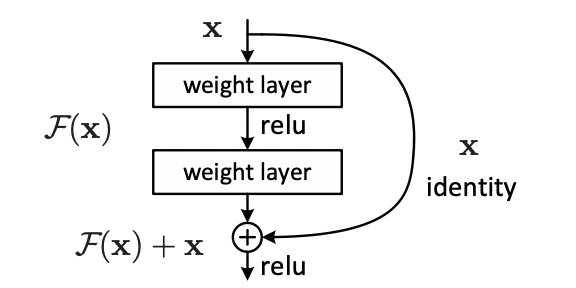
\includegraphics[width=0.35\linewidth]{./figures/01-chapter1/resnetBlock} 

}

\caption{Figure 1. Building block of residual learning}\label{fig:ch01-figure01}
\end{figure}

The function \(F \left( x,\left\{ W_i\right\} \right)\) represents the residual mapping that is to be learned. For the example with two layers from Fig.1 that has two layers, \(F = W_2\sigma\left( W_1x\right)\) in which \(\sigma\) denotes the ReLU activation function, and to simplify the notations, biases are left out. The operation \(F + x\) is conducted with a shortcut connection and element-wise addition. Afterward, He et al.~applied second nonlinearity ( i.e., \(\sigma \left( y \right)\), Fig.1).

The shortcut connections in Eq. (1) neither adds an extra parameter nor increases computation complexity, which enables comparisons between plain and residual networks that concurrently have the same number of parameters, depth, width, and computational cost (except for the negligible element-wise addition).
Dimensions of x and F must be equal in Eq. (1). Alternatively, to match the dimensions, linear projection \(W_s\) by the shortcut connections can be applied:

\begin{equation}
\tag{2}
y = F  \left( x,\left\{  W_i\right\} \right)+ W_sx.
\end{equation}

The square matrix \(W_s\) can be used in Eq. (1). However, experiments showed that identity mapping is enough to solve the degradation problem. Therefore, \(W_s\) only aims to match dimensions. Although more levels are possible, it was experimented with function F having two or three layers without stating the exact form of it. Assuming F only has one layer, Eq (1) it is comparable to a linear layer: \(y = W_1 x + x\). The theoretical notations are about fully-connected layers, but convolutional layers were used. The function \(F \left( x,\left\{ W_i\right\} \right)\) can be applied to represent multiple convolutional layers. Two feature maps are added element-wise, channel by channel.

\hypertarget{network-architectures}{%
\subsubsection{Network Architectures}\label{network-architectures}}

To construct efficient residual network, various plain/residual networks were tested. They trained the network on benchmarked datasets, one of them being the ImageNet dataset, which will be used for a comparison of network architectures. Fig. 2 shows that every residual network needs a plain baseline network inspired by the VGG network \citet{vgg} on which identity mapping by shortcuts is applied.

\emph{Plain Network} The philosophy of VGG nets 41 mainly inspires plain baselines. There are two rules that convolution layers, which usually have 3x3 filters, follow:

\begin{itemize}
\tightlist
\item
  feature maps with the same output size have the same number of layers;
\item
  reducing the size of a feature map by half doubles the number of filters per layer to maintain time complexity per layer
\end{itemize}

Convolutional layers with a stride of 2 perform downsampling directly. A global average pooling layer and a 1000-way fully-connected layer with softmax are at the end of the network. The number of weighted layers sums up to 34 in Fig. 2 (middle).Compared to VGG nets, this model has fewer filters and lower complexity. (Fig. 2, left).

\emph{Residual Network} Based on the above plain network, additional shortcut connections (Fig. 2, right) turn the network into its associate residual variant. The identity shortcuts (Eq. (1)) can be directly used in the case of the exact dimensions of the input and output (solid line shortcuts in Fig. 2). For the different dimensions (dotted line shortcuts in Fig. 2), two options are considered:

\begin{itemize}
\tightlist
\item
  The shortcut still performs identity mapping, but with extra zero entries padded to cope with the increasing dimensions, without adding new parameters;
\item
  The projection shortcut in Eq. (2) matches dimensions (due to 1×1 convolutions).
\end{itemize}

In both cases, shortcuts will be done with a stride of two when they go across feature maps of two sizes.

\begin{figure}

{\centering 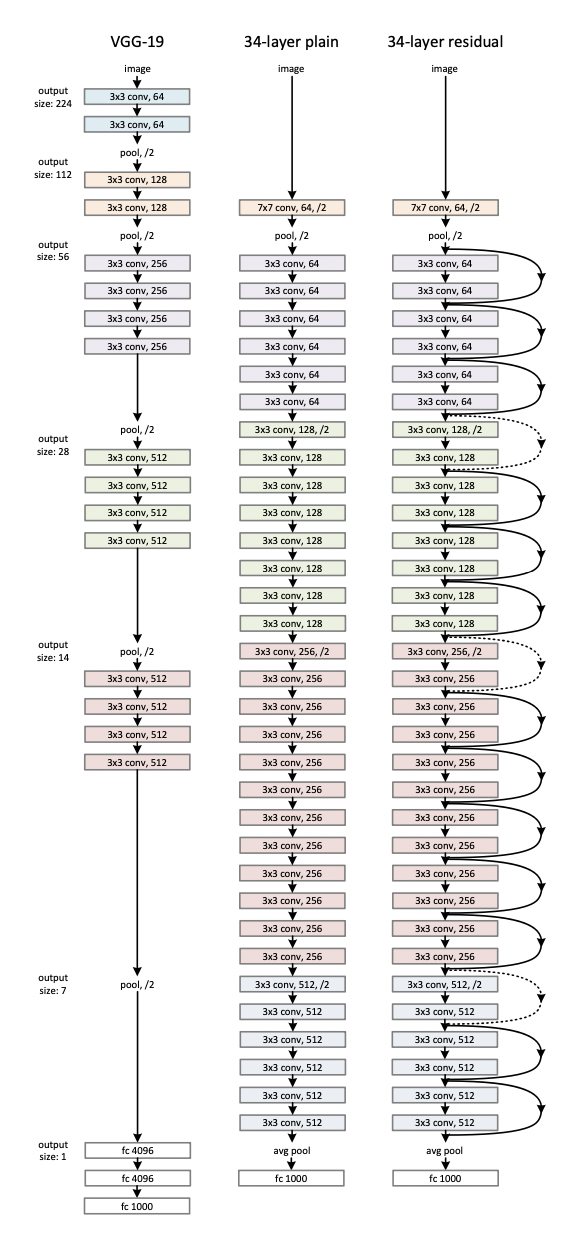
\includegraphics[width=1\linewidth]{./figures/01-chapter1/ResNet_architecture} 

}

\caption{Figure 2. Architecture of ResNet}\label{fig:ch01-figure02}
\end{figure}

\hypertarget{efficientnet}{%
\subsection{EfficientNet}\label{efficientnet}}

Until Tan M. introduced EfficientNet \citet{effecient}, it was popular to scale only one of the three dimensions -- depth, width, or image size. The empirical study shows that it is critical to balance all network dimensions, which can be achieved by simply scaling each with a constant ratio. Based on this observation, a simple yet effective compound scaling method was proposed, which uniformly scales network width, depth, and resolution with a set of fixed scaling coefficients.
For example, if 2N times more computational resources are available. In that case, increasing the network depth by \(\alpha N\), width by \(\beta N\), and image size by \(\gamma N\) would be possible.Here \(\alpha,\beta,\gamma\) are constant coefficients determined by a small grid search on the original miniature model. Fig. 3 illustrates the difference between this scaling method and conventional methods.
A compound scaling method makes sense if an input image is bigger since a larger receptive field requires more layers and more significant channel features to capture fine-grained patterns. Theoretically and empirically, there has been a special relationship between network width and depth \citet{depthwidth}. Existing MobileNets \citet{mobilenet} and ResNet are used to demonstrated new scaling method.

\begin{figure}

{\centering 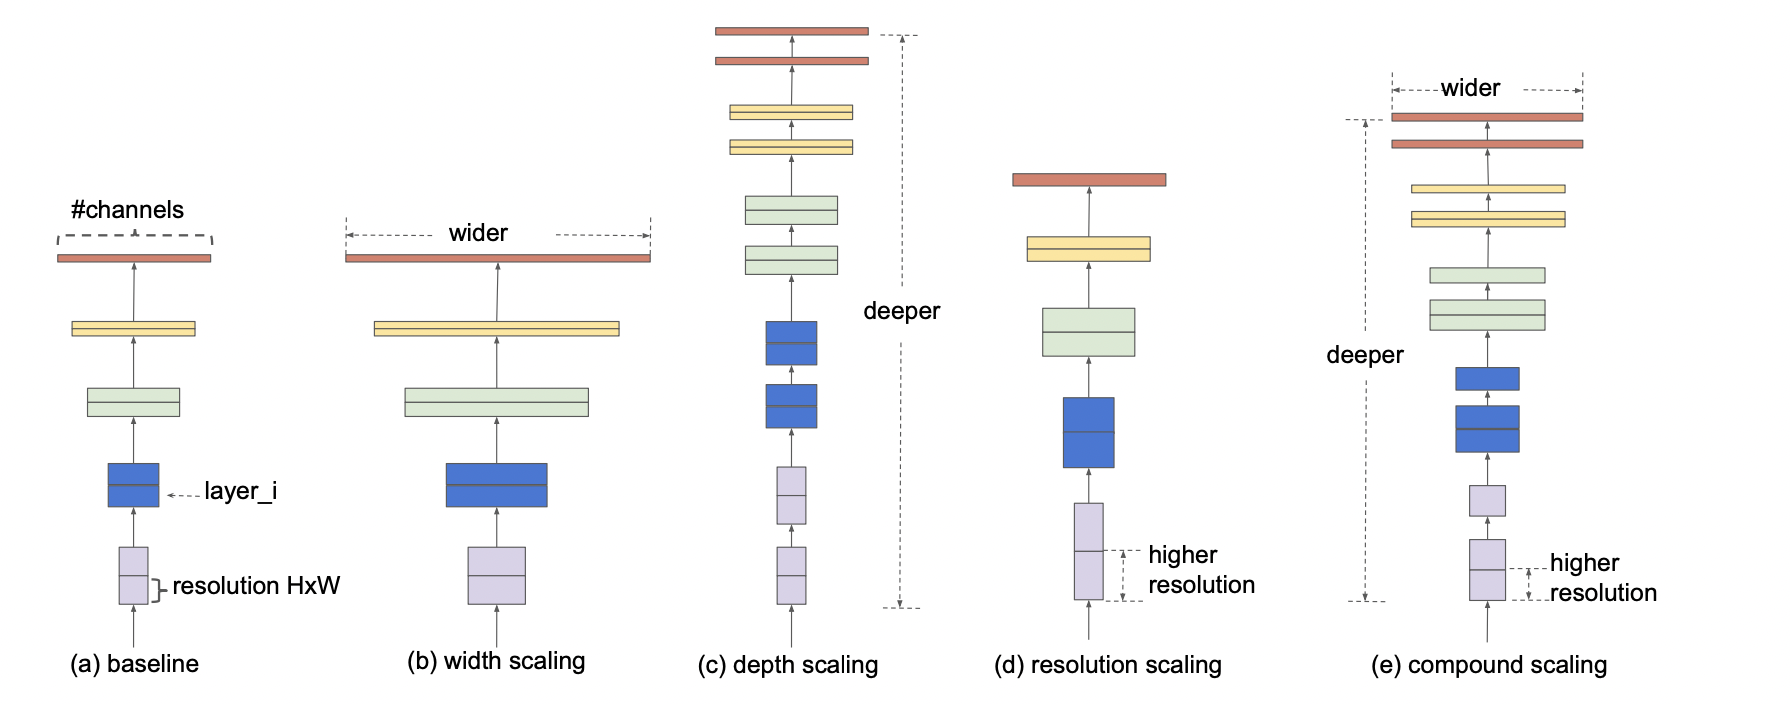
\includegraphics[width=1\linewidth]{./figures/01-chapter1/Model_scaling} 

}

\caption{Figure 3. Model scaling}\label{fig:ch01-figure03}
\end{figure}

\hypertarget{compound-model-scaling}{%
\subsubsection{Compound Model Scaling}\label{compound-model-scaling}}

\hypertarget{problem-formulation}{%
\paragraph{Problem Formulation}\label{problem-formulation}}

A function \(Y_i = \mathcal{F}i \left( X_i \right)\) with the operator \(\mathcal{F}_i\), output tensor \(Y_i\), input tensor \(X_i\) of shape \(\left( H_i, W_i, C_i \right)\), spatial dimensions \(H_i\), \(W_i\), and channel dimension \(C_i\) is called a ConvNet Layer \(i\). A ConvNet N appears as a list of composing layers:
\begin{equation}
\tag{3}
\mathcal{N}=\mathcal{F_k}\odot \cdots \mathcal{F_2}\odot\mathcal{F_1}\left( X_1 \right)=\bigodot{j=1\cdots k}\mathcal{F_j}\left( X_1 \right)
\end{equation}

Effectively, these layers are often partitioned into multiple stages, and all layers in each stage share the same architecture. For example, ResNet has five stages, with all layers in every stage being the same convolutional type, except for the first layer that performs down-sampling. Therefore, a ConvNet can be defined as:

\begin{equation}
\tag{4}
 \mathcal{N}=\bigodot_{i=1\cdots s}\mathcal{F_i}^{L_i}\left( X_{\left( H_i, W_i, C_i  \right)} \right)
\end{equation}

where \(\mathcal{F_i}^{L_i}\) denotes layer \(\mathcal{F_i}\) which is repeated \(L_i\) times in stage \(i\), and \(\left( H_i, W_i, C_i \right)\) is the shape of input tensor \(X\) of layer \(i\).

In comparison to the regular ConvNet focusing on best layer architecture \(\mathcal{F_i}\) search, model scaling centers on the expansion of the network length \(\left( L_i\right)\), width \(\left( C_i \right)\), and/or resolution \(\left( H_i, W_i\right)\) without changing \(\mathcal{F_i}\) that was predefined in the baseline network. Although model scaling simplifies the design problem of the new resource constraints through the fixing \(\mathcal{F_i}\), different \(\left( L_i, H_i, W_i, C_i \right)\) for each layer, the large designe space remains to be explored. To further reduce design space, all layers are restricted to be scaled uniformly with a constant ratio. In this case, the goal is to maximize the model's accuracy for any given resource constraints, which can be presented as an optimization problem:

\begin{equation}
\tag{5}
\max_{d,w,r}  Accuracy \left( \mathcal{N}\left( d,w,r \right) \right) \\
s.t.\mathcal{N}\left( d,w,r \right)=\bigodot_{I=1...s}\hat{\mathcal{F}}{i}^{d\cdot \hat{L{i}}}\left( X_{\left\langle r\cdot \hat{H_i},r\cdot \hat{W_i},w\cdot \hat{C_i}\right\rangle} \right) \\
Memory\left( \mathcal{N} \right)≤ targetMemory \\
FLOPS\left( \mathcal{N} \right) ≤ targetFlops \\
\end{equation}
where w,d,r are coefficients for scaling network width, depth, and resolution; \(\left(\widehat{\mathcal{F}}_i, \widehat{L}_i, \widehat{H}_i, \widehat{W}_i, \widehat{C}_i \right)\) are predefined parameters in baseline network.

\hypertarget{scaling-dimensions}{%
\paragraph{Scaling Dimensions}\label{scaling-dimensions}}

The main difficulty of this optimization problem is that the optimal \emph{d, w, r} depend on each other, and the values change under different resource constraints. Due to this difficulty, conventional methods mostly scale ConvNets in one of these dimensions:

\textbf{Depth (\(d\)):} One of the most significant networks previously described as ResNet. As it was described, the problem of ResNets is that accuracy gain of a very deep network diminishes. For example, ResNet-1000 has similar accuracy to ResNet-101 even though it has many more layers.

\textbf{Width (\(w\)):} Scaling network width is commonly used for small-size models. However, wide but shallow networks tend to have difficulty grasping higher-level features.

\textbf{Resolution (\(r\)):} Starting from 224x224 in early ConvNets, modern ConvNets tend to use 299x299 or 331x331 for better accuracy. GPipe \citet{gpipe} recently achieved state-of-the-art ImageNet accuracy with 480x480 Resolution. Higher resolutions, such as 600x600, are also widely used in object detection ConvNets.

The above analyses lead to the first observation:

\textbf{Observation 1:} Scaling up any network width, depth, or resolution dimension improves accuracy, without gain diminishes for bigger models.

\hypertarget{compound-scaling}{%
\paragraph{Compound Scaling}\label{compound-scaling}}

Firstly, it was observed that different scaling dimensions are not independent because higher resolution images require increased network depth. The larger receptive fields can help capture similar features that include more pixels in bigger images. Similarly, network width should be increased when the resolution is higher to capture more fine-grained patterns. The intuition suggests that different scaling dimensions should be coordinated and balanced rather than conventional scaling in single dimensions.
To confirm this thought, results of networks width \(w\) without changing depth (\(d\)=1.0) and resolution (\(r\)=1.0) were compared with deeper (\(d\)=2.0) and higher resolution (\(r\)=2.0) networks. This showed that width scaling achieves much better accuracy under the same FLOPS cost. These results lead to the second observation:

\textbf{Observation 2:} To achieve better accuracy and efficiency, balancing all network width, depth, and resolution dimensions during ConvNet scaling is critical. Earlier researches have tried to arbitrarily balance network width and depth, but they all require tedious manual tuning.

A new \textbf{compound scaling method}, which uses a compound coefficient \(\varphi\) to uniformly scale network width, depth, and resolution in a principled way, was proposed.

\begin{equation}
\tag{6}
depth: \mathcal{d}=\alpha^{\varphi} \\
width: \mathcal{w}=\beta^{\varphi}\\
resolution: \mathcal{r}=\gamma^{\varphi}\\
s.t.  \alpha\cdot \beta^{2}\cdot \gamma^{2}\approx 2\\
 \alpha \ge 1, \beta \ge 1, \gamma \ge 1\\
\end{equation}

where \(\alpha, \beta, \gamma\) are constants that can be determined by a small grid search, \(\varphi\) is a user-specified coefficient that controls how many more resources are available for model scaling, while \(\alpha, \beta, \gamma\) specify how to assign these extra resources to network width, depth, and resolution, respectively. Notably, the FLOPS of a regular convolution op is proportional to \(d, w^{2}, r^{2}\), i.e., doubling network depth will double FLOPS, but doubling network width or Resolution will increase FLOPS by four times. Scaling a ConvNet with previous equation will approximately increase total FLOPS by \(\left( \alpha\cdot \beta^{2}\cdot \gamma^{2} \right)^{\varphi}\). In this paper, \(\alpha\cdot \beta^{2}\cdot \gamma^{2}\approx 2\) is constrain such that for any new \(\varphi\), the total FLOPS will approximately increase by \(2\varphi\)

\hypertarget{efficientnet-architecture}{%
\subsubsection{EfficientNet Architecture}\label{efficientnet-architecture}}

A good baseline network is essential because model scaling does not affect its layer operators \(F*[i]\). Therefore this method is also estimated on ConvNets.
A new mobile-sized baseline called EfficientNet was developed to show the effectiveness of the new scaling method. Metrics that were used to estimate the efficacy are accuracy and FLOPS.
The baseline efficient network that was created is named EfficientNet-B0. Afterward, this compound scaling method is applied in two steps:

\begin{itemize}
\item
  \textbf{STEP 1}: By fixing \(\varphi = 1\) and, assuming twice more resources available, a small grid search of \$\alpha, \beta, \gamma \$ based Eq. (6) showed that the best values for EfficientNet-B0 are \(\alpha = 1.2, \beta = 1.1, \gamma=1.15\), under constraint of \(\alpha·\beta^2·\gamma^2 ≈2\).
\item
  \textbf{STEP 2}: Afterward fix \(\alpha,\beta,\gamma\) as constants and scale up the baseline network with different \(\varphi\) using Eq.(6) to construct EfficientNet-B1 to B7
\end{itemize}

\begin{longtable}[]{@{}cc@{}}
\toprule
Name & Number of parameters\tabularnewline
\midrule
\endhead
EfficientNet-B0 & 5.3M parameters\tabularnewline
EfficientNet-B1 & 7.8M parameters\tabularnewline
EfficientNet-B2 & 9.2M parameters\tabularnewline
EfficientNet-B3 & 12M parameters\tabularnewline
EfficientNet-B4 & 19M parameters\tabularnewline
EfficientNet-B5 & 30M parameters\tabularnewline
EfficientNet-B6 & 43M parameters\tabularnewline
EfficientNet-B7 & 66M parameters\tabularnewline
\bottomrule
\end{longtable}

Indeed, even better performance is achievable by searching for \(\alpha,\beta,\gamma\) directly around a large model, but the search cost becomes prohibitively more expensive on larger models. This method searches once on a small baseline network, then scales the coefficient for all other models.

\hypertarget{results-and-comparison-of-the-networks}{%
\subsection{Results and comparison of the networks}\label{results-and-comparison-of-the-networks}}

To demonstrate the performance of both networks, ResNet and EfficientNets were trained and evaluated on the benchmark ImageNet 2012 classification dataset consisting of 1000 classes.
Since deeper scaling should provide better results in the case of ResNet, it was trained with increased depth each time. First meaningful results were obtained in ResNet-34, which peformed better than plain-34 baseline by 3,5\% when top-1 acc. is compared. They also compared tree versions of ResNet: (A) zero-padding shortcuts, for increasing dimensions, and all shortcuts are parameter-free (B) projection shortcuts, for increasing dimensions, and other shortcuts are identity; and (C) all shortcuts are projections. Each version improved both top-1 and top-5 accuracy.
Afterward, the depth of the network was increased and ResNet-50, ResNet-101, and ResNet-152 were created. Each increase in depth leads to higher accuracy. In deeper models, the trade-off between accuracy increase and deeper model is not worth describing. All results are shown in the table below.

\begin{longtable}[]{@{}ccc@{}}
\toprule
Model & top-1 acc. & top-5 acc.\tabularnewline
\midrule
\endhead
VGG-16 & 71.93 & 90.67\tabularnewline
GoogLeNet & - & 90.85\tabularnewline
plain-34 & 71.46 & 89.98\tabularnewline
ResNet-34 A & 74.97 & 92.24\tabularnewline
ResNet-34 B & 75.48 & 92.54\tabularnewline
ResNet-34 C & 75.81 & 92.6\tabularnewline
ResNet-50 & 77.15 & 93.29\tabularnewline
ResNet-101 & 78.25 & 93.95\tabularnewline
ResNet-152 & \textbf{78.57} & \textbf{94.29}\tabularnewline
\bottomrule
\end{longtable}

In the case of EfficientNets, the results achieved by the previous state-of-the-art networks on the same ImageNet dataset were aimed to improve. Among all state-of-the-art networks, EfficientNets were compared with ResNets-50 and ResNet-152. They compared the results of networks derivated by changing scaling parameters EfficientNet-B0 to EfficientNet-B7. The results of each network were better than the previous one. Also, they have shown that EfficientNet-B0 outperforms ResNet-50 and that EfficientNet-B1 outperforms ResNet-152. This means that scaling through all three dimensions can provide better results than scaling through just one dimension. The drawback of this approach is the computational power, which makes it less popular than previous methods. Again, all results are shown in the table below.

\begin{longtable}[]{@{}ccc@{}}
\toprule
Model & top-1 acc. & top-5 acc.\tabularnewline
\midrule
\endhead
EfficientNet-B0 ResNet-50 & 77.1 76 & 93.3 93\tabularnewline
EfficientNet-B1 ResNet-152 & 79.1 77.8 & 94.4 93.8\tabularnewline
EfficientNet-B2 & 80.1 & 94.9\tabularnewline
EfficientNet-B3 ResNeXt-101 & 81.6 80.9 & 95.7 95.6\tabularnewline
EfficientNet-B4 & 82.9 & 96.4\tabularnewline
EfficientNet-B5 & 83.6 & 96.7\tabularnewline
EfficientNet-B6 & 84 & 96.8\tabularnewline
EfficientNet-B7 GPipe & \textbf{84.3} 84.3 & \textbf{97} 97\tabularnewline
\bottomrule
\end{longtable}

\hypertarget{contrastive-learning}{%
\subsection{Contrastive learning}\label{contrastive-learning}}

In recent years the problem of classification of the unlabeled dataset is becoming more widespread. More unlabeled datasets are being created in fields like medicine, the automotive industry, military, etc., requiring human labeling. Since the process is expensive and time-consuming, researchers assumed, it could be automated with contrastive learning frameworks. One of the first and most known contrastive learning frameworks is SimCLR \citet{SimCLR}. The advantage of this framework is its simplicity, yet it achieves high accuracy on classification tasks. The main idea is to have two copies of the image, which are then used to train two networks and later compared. The problem with this framework is that it doubles the size of the dataset and reaches among all images, which can be computationally unfeasible in large datasets. Bootstrap Your Own Latent \citet{BYOL} was introduced to avoid making double-sized datasets. The idea was to bootstrap images' representations, avoiding unnecessary image comparison. These two frameworks will be described in this work.
Further improvements in the choice of creating two views of images and comparison techniques were presented in different frameworks such as Nearest-Neighbor Contrastive Learning (NNCLR) \citet{NNCLR}, Open World Object Detection (ORE) \citet{ORE}, Swapping Assignments between multiple Views (SwAV) \citet{SwAV}, and many more.
This field is a constant research topic, and new, improved frameworks are being created to help researchers solve other tasks requiring labeled datasets.

\hypertarget{a-simple-framework-for-contrastive-learning-of-visual-representations}{%
\subsection{A Simple Framework for Contrastive Learning of Visual Representations}\label{a-simple-framework-for-contrastive-learning-of-visual-representations}}

Chen T. et al.~intended to analyze and describe a better approach to learning visual representations without human supervision. They have introduced a simple framework for contrastive learning of visual representations and called it SimCLR \citet{SimCLR}. As they claim, SimCLR outperforms previous work, is more straightforward, and does not require a memory bank.

Intending to understand what qualifies good contrastive representation learning, the significant components of the framework were studied and resulted in:

\begin{itemize}
\tightlist
\item
  A contrastive prediction task requires combining multiple data augmentation operations, which results in effective representations. Unsupervised contrastive learning benefits from more significant data augmentation.
\item
  The quality of the learned representations can be substantially improved by introducing a learnable nonlinear transformation between the representation and the contrastive loss.
\item
  Representation learning with contrastive cross-entropy loss can be improved by normalizing embeddings and adjusting the temperature parameter appropriately.
\item
  Unlike its supervised counterpart, contrastive learning benefits from larger batch sizes and extended training periods. Contrastive learning also benefits from deeper and broader networks, just as supervised learning does.
\end{itemize}

\hypertarget{the-contrastive-learning-framework}{%
\subsubsection{The Contrastive Learning Framework}\label{the-contrastive-learning-framework}}

Like previous contrastive learning algorithms, in the SimCLR, a contrastive loss is used to learn representations by maximizing agreement between various augmented views of the same data example. This framework contains four significant components, which are shown in Fig. 4:

\begin{enumerate}
\def\labelenumi{\arabic{enumi}.}
\item
  A stochastic \emph{data augmentation} module
\item
  A neural network \emph{base encoder}
\item
  A small neural network \emph{projection head}
\item
  A \emph{contrastive loss function}
\end{enumerate}

\begin{figure}

{\centering 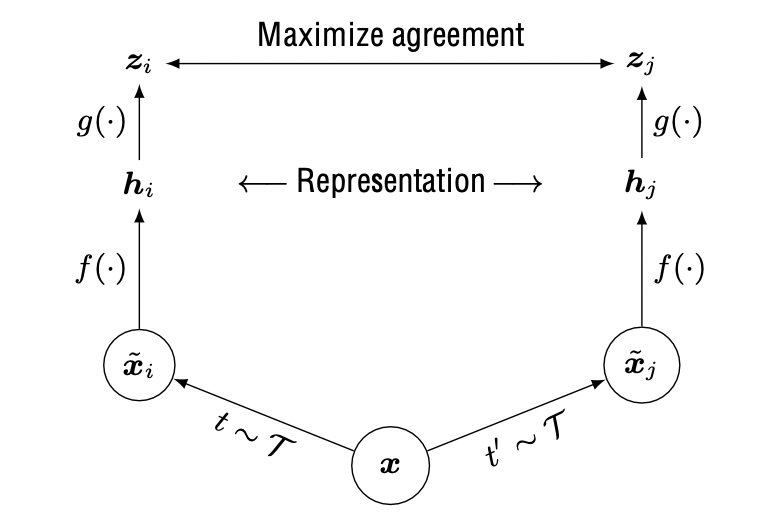
\includegraphics[width=0.3\linewidth]{./figures/01-chapter1/SimCLR} 

}

\caption{Figure 4. A simple framework for contrastive learning of visual representations}\label{fig:ch01-figure04}
\end{figure}

\hypertarget{stochastic-data-augmentation-module}{%
\paragraph{Stochastic data augmentation module}\label{stochastic-data-augmentation-module}}

First, the minibatch of N examples is sampled randomly, and the contrastive prediction task is defined on pairs of augmented examples, resulting in 2N data points. A memory bank was not used to train the model, instead, the training batch size varied from 256 to 8192.
Any given data example randomly returns two correlated views of the same example, denoted \(\tilde{x}_{i}\) and \(\tilde{x}_{j}\), which is known as a \textbf{positive pair}. \textbf{Negative pairs} are all other \(2(N-1)\) pairs except the positive pair. In one view, some data augmentation techniques are applied.
Data augmentation is widely embraced in supervised and unsupervised representation learning. Unfortunately, it has not been used to define the contrastive prediction task, which is mainly determined by changing the architecture. It was shown that choosing different data augmentation techniques can reduce the complexity of previous contrastive learning frameworks.
There are many data augmentation operations, the focus was on the most common ones, which are:

\begin{itemize}
\tightlist
\item
  \textbf{spatial geometric transformation}: cropping and resizing (with horizontal flipping), rotation and cutout,
\item
  \textbf{appearance transformation}: color distortion (including color dropping), brightness, contrast, saturation, Gaussian blur, and Sobel filtering.
\end{itemize}

\begin{figure}

{\centering 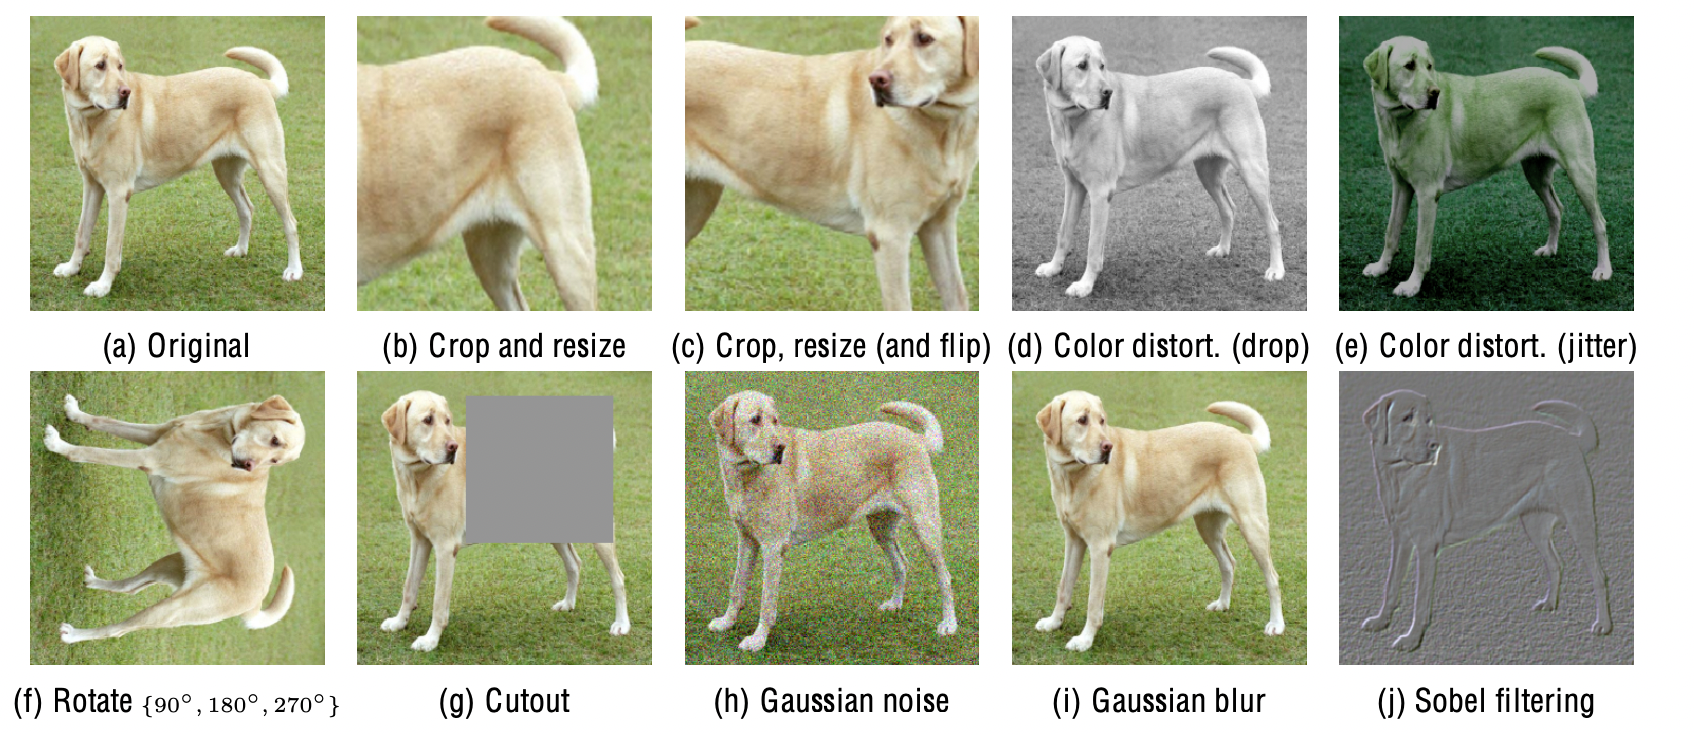
\includegraphics[width=0.8\linewidth]{./figures/01-chapter1/augmentation} 

}

\caption{Figure 5. Augmentation texhniques}\label{fig:ch01-figure05}
\end{figure}

Due to the image sizes in the ImageNet dataset, all images were always randomly cropped and resized to the same resolution. Later on, other targeted data augmentation transformations were applied to one branch, remaining the one as original i.e.~\(t\left( x_{i}\right)= x_i\).
Applying just individual transformation is insufficient for the model to learn good representations. The model's performance improves after composing augmentations, although the contrastive prediction task becomes more complex. The composition of augmentations that stood out were random cropping and random color distortion.

It was also observed that stronger color augmentation significantly improves the linear evaluation of unsupervised learned models. Stronger color augmentations do not enhance the performance of supervised models when trained with the same augmentations. Based on the experiments, unsupervised contrastive learning benefits from stronger color data augmentation than supervised learning.

\hypertarget{neural-network-base-encoder}{%
\paragraph{Neural network base encoder}\label{neural-network-base-encoder}}

Neural network based encoder \(f\left( \cdot \right)\) extracts representation vectors from augmented data examples. This framework does not restrict a choice of the network architecture, although for simplicity the commonly used ResNet was picked and obtained \(h_i=f\left( \tilde{x}_{i} \right)=ResNet\left(\tilde{x}_{i}\right)\) where \(\textbf{h}_i\in \mathbb{R}^{d}\) is the output after the average pooling layer. Although increasing depth and width improves performance, the ResNet-50 was chosen. Furthermore, when the model size increases, the gap between supervised and unsupervised learning shrinks, suggesting that bigger models benefit from unsupervised learning more.

\hypertarget{small-neural-network-projection-head}{%
\paragraph{Small neural network projection head}\label{small-neural-network-projection-head}}

A small neural network projection heads \(g\left( \cdot \right)\) that maps representations to the space where contrastive loss is applied. The importance of including a projection head, i.e., \(g\left( h \right)\) was evaluated. They have considered three different architectures for the head:

\begin{enumerate}
\def\labelenumi{\arabic{enumi}.}
\tightlist
\item
  identity mapping,
\item
  linear projection,
\item
  the default nonlinear projection with one additional hidden layer and ReLU activation function.
\end{enumerate}

The results showed that a nonlinear projection head is better than a linear projection and much better than no projection. It improves the representation quality of the layer before it. They have used a MLP with one hidden layer to obtain \(z_i = g\left( \textbf{h}_i \right) = W^{\left( 2\right)}\sigma \left( W^{\left( 1\right)} \textbf{h}_i\right)\) where \(\sigma\) is a ReLU non-linearity.

This step is performed because defining the contrastive loss on \(z_i\) instead of on \(\textbf{h}_i\) would not lead to loss of information caused by contrastive loss. Especially, \(z=g\left( h \right)\) is trained to be invariant to data transformations. As a result, \(g\) can remove information useful for a downstream task, such as object color or orientation. Using the nonlinear transformation \(g\left( * \right)\), \(h\) can maintain and form more information.

\hypertarget{contrastive-loss-function}{%
\paragraph{Contrastive loss function}\label{contrastive-loss-function}}

Given a set \(\left\{ \tilde{x}_{ik} \right\}\) including a positive pair of examples \(\tilde{x}_{i}\) and \(\tilde{x}_{j}\), the contrastive prediction task aims to identify \(\tilde{x}_{i}\) in \(\left\{ \tilde{x}_{i} \right\}_{k\neq i}\) for a given \(\tilde{x}_{i}\). In the case of positive examples, the loss function is as follows \(\left( i, j\right)\) is defined as

\begin{equation}
\tag{7}
\mathcal{l}_{i,j} = −\log\frac{exp\left( \frac{sim(z_i,z_j)}{\tau} \right)}{\sum_{k=1}^{2N}\mathbb{I_{\left[ k\neq i \right]}}exp\left( \frac{sim(z_i,z_k)}{\tau} \right)}
\end{equation}

where \(\mathbb{I_{\left[ k\neq i \right]}}\in\left\{ 0,1 \right\}\) is an indicator function, \(\tau\) denotes a temperature parameter and \(sim\left(\textbf{u,v} \right)= \frac{\textbf{u}^T\textbf{v}}{\left\| \textbf{u}\right\|\left\| \textbf{v} \right\|}\) is a dot product between \(\mathcal{l}_2\) normalized \(\textbf{u},\textbf{v}\).

The final loss is calculated across all positive pairs, both \(\left( i,j \right)\) and \(\left( j,i \right)\), in a mini-batch. It was named \textbf{NT-Xent}, the normalized temperature-scaled cross-entropy loss.

The NT-Xent loss was compared against other commonly used contrastive loss functions, such as logistic loss and margin loss. Gradient analysis shows that \(l_2\) normalization, cosine similarity, and temperature together effectively weight different examples, and a suitable temperature can make the model learn from hard negatives. The advantage of NT-Xent is that it weights the negatives by their relative hardness. Without normalization and proper temperature scaling, performance is significantly worse. Also, the contrastive task accuracy is higher, but the resulting representation is worse under linear evaluation.

\hypertarget{bootstrap-your-own-latent}{%
\subsection{Bootstrap Your Own Latent}\label{bootstrap-your-own-latent}}

The fundamental idea of contrastive learning is to create pairs of images on which the framework would be trained. Creating negative pairs relies on large batch sizes, memory banks, or customized mining strategies which can be challenging in larger datasets. Grill J.B. at al.~wanted to create a new approach that would achieve better performance than other contrastive methods without using negative pairs. A solution they have introduced is a method called Bootstrap Your Own Latent (BYOL) \citet{BYOL}. The idea was to bootstrap representations of images. As a result, BYOL is more robust to the choice of image augmentations.
Furthermore, BYOL has two neural networks, called online and target networks, which interact and learn from each other. Using an augmented view of an image, BYOL trains its online network to predict the target network's representation of another augmented view. This approach achieved state-of-the-art results when trained on the ImageNet dataset under the linear evaluation protocol. Additionally, compared to SimCLR, a strong contrastive baseline, BYOL suffers from much less performance drop when only random crops are used to augment images.

\hypertarget{description-of-method}{%
\subsubsection{Description of method}\label{description-of-method}}

BYOL aims to learn a representation of \(y_\theta\). It uses two neural networks: \emph{online} and \emph{the target network} to achieve that. The \emph{online network} is determined by a set of weights \(\theta\) and consists of:

\begin{itemize}
\tightlist
\item
  an encoder \(f_\theta\),
\item
  a projector \(g_\theta\),
\item
  a predictor \(q_\theta\).
\end{itemize}

\begin{figure}

{\centering 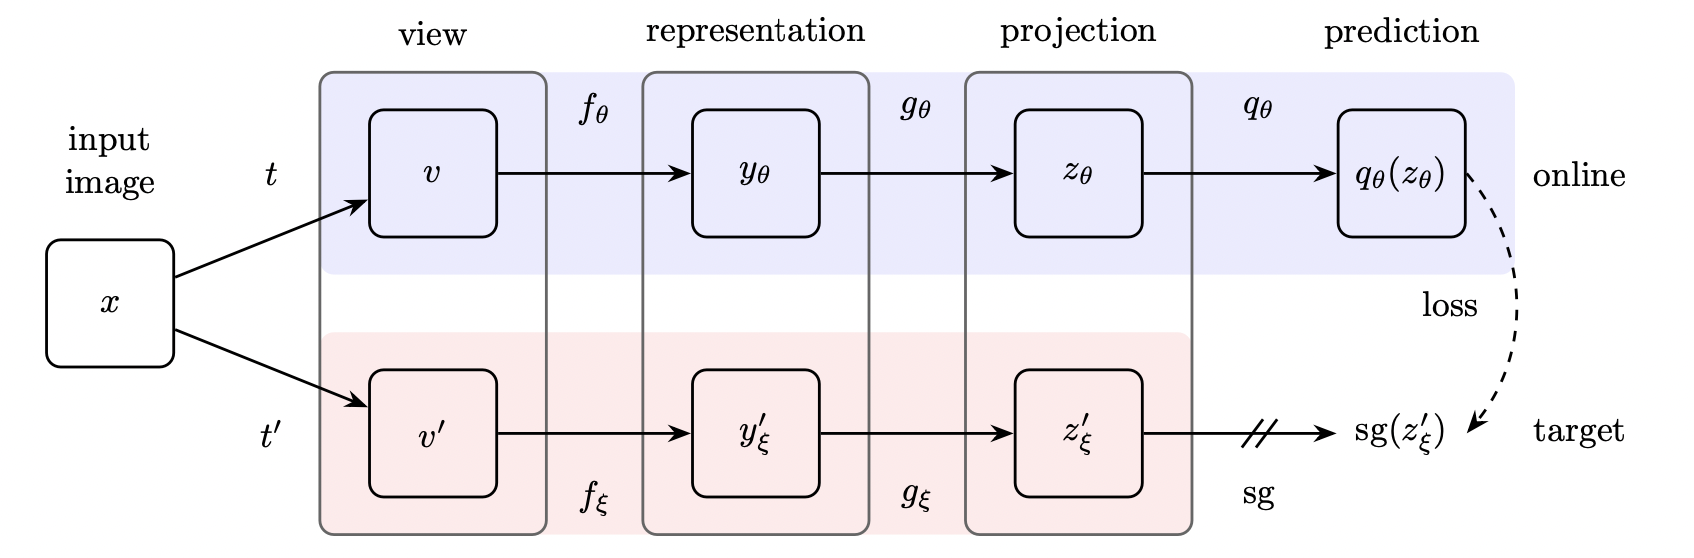
\includegraphics[width=0.8\linewidth]{./figures/01-chapter1/BYOL} 

}

\caption{Figure 6. Bootstrap Your Own Latent}\label{fig:ch01-figure06}
\end{figure}

The \emph{target network} has the same architecture as the online network but uses different weights \(\xi\). It provides the regression targets to train the online network, and its parameters \(\xi\) are an exponential moving average of the online parameters \(\theta\). Precisely, given a target decay rate \(\tau \in[0,1]\), after each training step, the following update
\begin{equation}
\tag{8}
\xi \leftarrow \tau \xi+(1-\tau) \theta
\end{equation}
is performed.
Firstly, image is sampled uniformly from \(\mathcal{D}\), from which two distributions of image augmentations \(\mathcal{T}\) and \(\mathcal{T}^{\prime}\) are created. BYOL applies respectively two image augmentations \(t \sim \mathcal{T}\) and \(t^{\prime} \sim \mathcal{T}^{\prime}\), creating two augmented views \(v \triangleq t(x)\) and \(v^{\prime} \triangleq t^{\prime}(x)\). First augmented view \(v\) is used at online network, resulting the output \(y_{\theta} \triangleq f_{\theta}(v)\) and afterwards projection \(z_{\theta} \triangleq g_{\theta}(y)\). Similarly, from second augmented view \(v^{\prime}\) the target network outputs \(y_{\xi}^{\prime} \triangleq f_{\xi}(v^{\prime})\) and the target projection \(z_{\xi}^{\prime} \triangleq g_{\xi}(y^{\prime})\). Later on output a prediction of \(q_{\theta}\left(z_{\theta}\right)\) of \(z_{\xi}^{\prime}\) and \(\ell_{2}\)-normalize both \(q_{\theta}\left(z_{\theta}\right)\) and \(z_{\xi}^{\prime}\) to

\begin{equation}
\tag{9}
\overline{q_{\theta}}\left(z_{\theta}\right) \triangleq q_{\theta}\left(z_{\theta}\right) /\left\|q_{\theta}\left(z_{\theta}\right)\right\|_{2} \quad \textrm{and} \quad
\bar{z}_{\xi}^{\prime} \triangleq z_{\xi}^{\prime} /\left\|z_{\xi}^{\prime}\right\|_{2}
\end{equation}

Predictor only applies to the online pipeline, making the architecture asymmetric between the online and target pipeline. Lastly, the following mean squared error between the normalized predictions and target projections is defined.

\begin{equation}
\tag{10}
\mathcal{L}_{\theta, \xi} \triangleq\left\|\overline{q_{\theta}}\left(z_{\theta}\right)-\bar{z}_{\xi}^{\prime}\right\|_{2}^{2}=2-2 \cdot \frac{\left\langle q_{\theta}\left(z_{\theta}\right), z_{\xi}^{\prime}\right\rangle}{\left\|q_{\theta}\left(z_{\theta}\right)\right\|_{2} \cdot\left\|z_{\xi}^{\prime}\right\|_{2}}
\end{equation}
Loss is symmetrized \(\mathcal{L}_{\theta, \xi}\) by using \(v^{\prime}\) for the online network and \(v\) for the target network separately to calculate \(\widetilde{\mathcal{L}}_{\theta, \xi}\). At each training step, a stochastic optimization step is applied to minimize \(\mathcal{L}_{\theta, \xi}^{\mathrm{BYOL}}=\mathcal{L}_{\theta, \xi}+\widetilde{\mathcal{L}}_{\theta, \xi}\) with respect to \(\theta\) only, but not \(\xi\). BYOL's dynamics are summarized as

\begin{equation}
\tag{11}
\theta \leftarrow \operatorname{optimizer}\left(\theta, \nabla_{\theta} \mathcal{L}_{\theta, \xi}^{\mathrm{BYOL}}, \eta\right)
\end{equation}

where \(\eta\) is a learning rate.
At the end of the training, only the encoder \(f_{\theta}\).

\hypertarget{comparison-of-contrastive-learning-frameworks}{%
\subsection{Comparison of contrastive learning frameworks}\label{comparison-of-contrastive-learning-frameworks}}

Of all frameworks, SimCLR is the most popular due to its simplicity. The ResNet-50 in 3 different hidden layer widths (width multipliers of 1×, 2×, and 4×) were used and trained for 1000 epochs each. The accuracy of these frameworks on the ImageNet dataset with few labels improved when the width of ResNet-50 increased. For SimCLR with ResNet-50 top-1 accuracy is 69.3 and top-5 accuracy is 89, while for ResNet-50(4x) top-1 accuracy is 85.8 and top-5 accuracy is 92.6. These results are comparable with supervised methods.
BYOL framework was built to improve the results of SimCLR. It was also stated that the accuracy for baseline ResNet-50 is 74.3 and 91.6 for top-1 accuracy and top-5 accuracy. When using ResNet-50(4x), accuracies increase to 78.6 and 94.2 for top-1 and top-5, respectively. More information about performance can be found in table below

\begin{longtable}[]{@{}ccccc@{}}
\toprule
Model & Architecture & Param (M) & top-1 acc. & top-5 acc.\tabularnewline
\midrule
\endhead
SimCLR & ResNet-50 & 24 & 69.3 & 89.0\tabularnewline
SimCLR & ResNet-50 (2x) & 94 & 74.2 & 93.0\tabularnewline
SimCLR & ResNet-50 (4x) & 375 & 76.5 & 93.2\tabularnewline
BYOL & ResNet-50 & 24 & 74.3 & 91.6\tabularnewline
BYOL & ResNet-50 (x2) & 94 & 77.4 & 93.6\tabularnewline
BYOL & ResNet-50 (x4) & 375 & 78.6 & 94.2\tabularnewline
BYOL & ResNet-200 (x2) & 250 & 79.6 & 94.8\tabularnewline
\bottomrule
\end{longtable}

\hypertarget{transformers-in-computer-vision}{%
\subsection{Transformers in Computer Vision}\label{transformers-in-computer-vision}}

Since the first appearance of the Transformers architecture in 2017 \citet{TRANSFORMERS_NLP}, it has become an irreplaceable part of all-natural language processing (NLP) models. The main advantage of Transformers is that they can be trained on a large text corpus and then fine-tuned on a smaller task-specific dataset, and this enabled model training of unspecified size with more than 100B parameters.

However, computer vision still relied on convolutional architectures. With datasets constantly growing and the diversity of the fields where computer vision tasks could be applied, researchers wanted to implement Transformers architecture in the CV field. Some works tried combining CNN-like architectures with self-attention \citet{wang}, and others attempted to replace convolutions entirely \citet{selfa}. Due to specialized attention patterns, the problem was that they have not yet been scaled effectively on modern hardware accelerators. Therefore, in large-scale image recognition, classic ResNet-like architectures are still state-of-the-art.

In 2021 Google research, Brain Team published the paper ``An image is worth 16x16 words,'' where they introduced new Transformers-based architecture for CV called Vision Transformers (ViT) \citet{vit}. Based on the success of Transformer in NLP scaling, they aimed to apply standard Transformer directly to images, changing it as little as possible. The image is split into patches, and linear embeddings of these patches are provided as inputs to the Transformer.
These patches are the same as tokens (eg. words) in NLP. The model is trained on image classification in a supervised fashion.

\hypertarget{vision-transformers}{%
\subsubsection{Vision Transformers}\label{vision-transformers}}

Brain Team wanted to create simple but universally scalable architecture to follow the original Transformers architecture.

\begin{figure}

{\centering 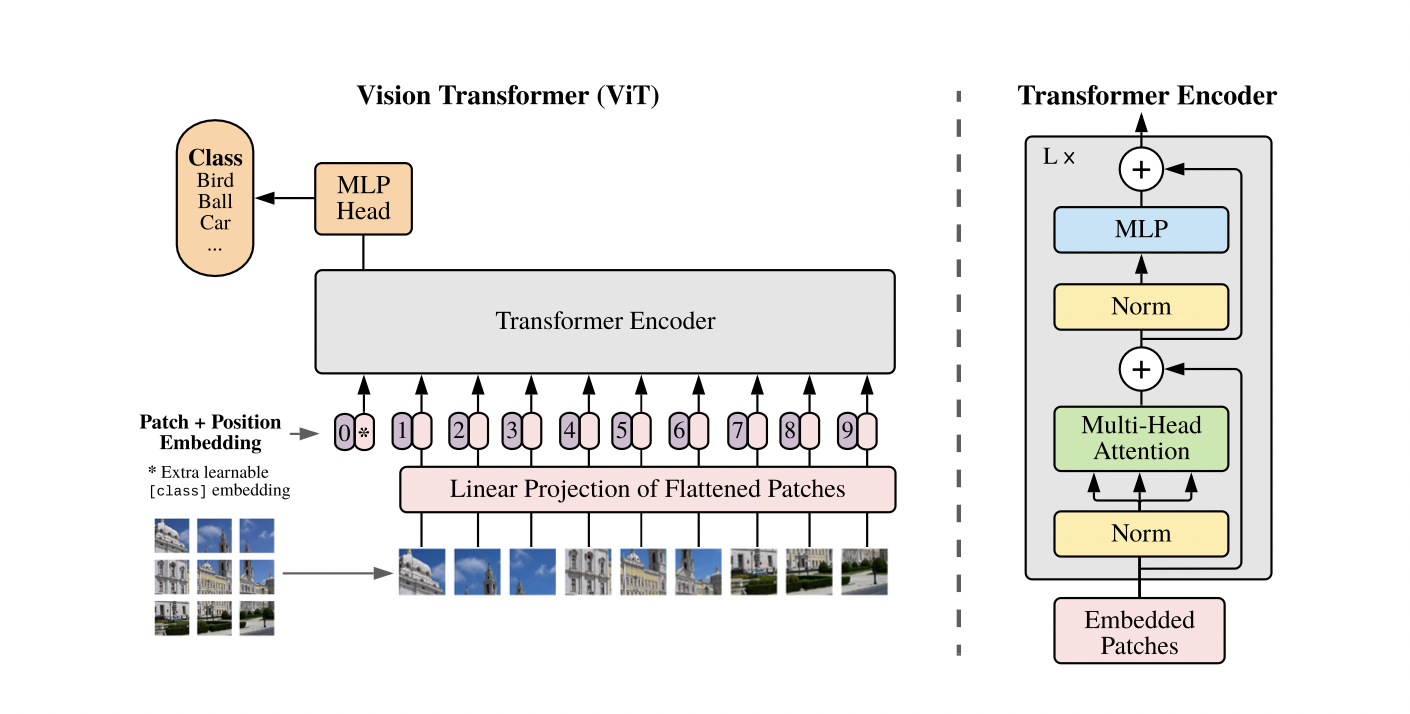
\includegraphics[width=0.9\linewidth]{./figures/01-chapter1/ViT} 

}

\caption{Figure 7. Vision Transformer}\label{fig:ch01-figure7}
\end{figure}

\hypertarget{method}{%
\paragraph{Method}\label{method}}

Compared to NLP, where the input of the Transformer is a 1D sequence of token embeddings, images are 2D objects. Firstly, images needed to be represented differently to imitate original architectures as closely as possible. For that reason image \(x\in \mathbb{R}^{ H \times W \times C}\) is reshaped into a sequence of flattened 2D patches \(x_p\in \mathbb{R}^{ N \times \left( P^2 \cdot C \right)}\), where \(\left(H,W\right)\) is the resolution of the original image, \(C\) is the number of channels,\(\left(P,P\right)\) is the resolution of each image patch, and \(N =HW/P^2\) is the resulting number of patches, also the Transformer's effective input sequence length. The Transformer input is a fixed through all layers vector size \(D\). The first step is to flatten the patches, usually 16x16, and map them to \(D\) dimensions with a trainable linear projection, creating patch embeddings.

\begin{equation}
\tag{12}
\mathbf{z}_{0} =\left[\mathbf{x}_{\text {class }} ; \mathbf{x}_{p}^{1} \mathbf{E} ; \mathbf{x}_{p}^{2} \mathbf{E} ; \cdots ; \mathbf{x}_{p}^{N} \mathbf{E}\right]+\mathbf{E}_{p o s}, \mathbf{E} \in \mathbb{R}^{\left(P^{2} \cdot C\right) \times D}, \mathbf{E}_{p o s} \in \mathbb{R}^{(N+1) \times D}
\end{equation}

To this sequence of ``patch embeddings,'' a prefix learnable {[}class{]} token, like in BERT, is usually added. This token \(\mathbf{z}_{0}^{0} = \mathbf{x}_{class}\) tells the model to classify the image and increases dimension of vector z. Also, the state of this token at the output of the Transformer encoder \(\left(\mathbf{z}_{L}^{0}\right)\), on which Layernorm is applied, serves as the image representation \(y\).

\begin{equation}
\tag{13}
\mathbf{y} =\operatorname{LN}\left(\mathbf{z}_{L}^{0}\right)
\end{equation}

Also, it is the only one to which the classification head is attached to during pre-training and fine-tuning. Classification head during pre-training is compiled of MLP with one hidden layer and a single linear layer at a fine-tuning time. Position embedding,a standard learnable 1D position embedding, are attached to the patch embeddings, serving as input to the encoder. The standard Transformer encoder consists of alternating layers of multiheaded self-attention and MLP blocks. After each block, a residual connection is applied.

\begin{equation}
\tag{14}
\mathbf{z}_{\ell}^{\prime} =\operatorname{MSA}\left(\operatorname{LN}\left(\mathbf{z}_{\ell-1}\right)\right)+\mathbf{z}_{\ell-1},  \ell=1 \ldots L
\end{equation}

\begin{equation}
\tag{15}
\mathbf{z}_{\ell} =\operatorname{MLP}\left(\mathrm{LN}\left(\mathbf{z}_{\ell}^{\prime}\right)\right)+\mathbf{z}_{\ell}^{\prime}, \ell=1 \ldots L
\end{equation}

Vision Transformer has a significantly lower inductive bias than CNNs in image-specific information. VIT only has local and translationally equivariant MLP layers, while the self-attention layers are global. Two-dimensional neighborhood structure is used sparingly: the image is cut into patches at the beginning, and the position embeddings are resized as needed at the fine-tuning time. Alternatively, the input sequence can consist of a CNN's feature maps on which patch embedding projection is applied.
Vision Transformers are pre-trained on large datasets, and fine-tuned to (smaller) downstream tasks. For fine-tuning projection head is removed and zero-initialized \(D \times K\) feedforward layer is attached, \(K\) being the number of downstream classes. It is also beneficial to use higher resolution then in pre-training. Also ViT can handle arbitrary sequence lengths, but the pre-trained position embeddings can become sufficient. It is necessary to point out that resolution adjustment and patch extraction are the only points at which an inductive bias about the 2D structure of the images is manually injected into the Vision Transformers

\hypertarget{experiments}{%
\paragraph{Experiments}\label{experiments}}

Similarly to BERT models, multiple versions of the model at various scales were created. They have created Base = ``B'', Large = ``L'', Huge = ``H'' versions of ViT, with 12, 24 and 32 layers and 86M, 307M and 632M parameters respectively.

To explore model scalability, the already mentioned dataset ImageNet was used. In addition, ViT was compared against slightly modified ResNet, creating ``ResNet(BiT)''. The batch Normalization layer was replaced with Group Normalization and used standardized convolutions. Another network that it was compared to was Noisy Student \citet{noisy}, a large EfficientNet. Experiments showed that ViT Hughe with 14x14 input patch size outperformed both CNN-based networks with an accuracy of 88.5\%, whereas ResNet BiT had 87.54\% and Noisy Student 88.4\%. Also, it is worth mentioning that ViT Large with 16x16 input patch size had 87.76\% accuracy on the same dataset.
Another thing worth pointing out is that ViT outperforms CNN-based architectures on all larger datasets yet performs slightly worse than CNN networks on a smaller dataset.

\hypertarget{conclusion}{%
\subsection{Conclusion}\label{conclusion}}

In this chapter, authors presented some of the current state-of-the-art approaches in Computer Vision. Nowdays, when technology is advancing each day, creating networks that would imitate human brain is more challenging. Still networks presented in this chapter are highly accurate and creating network which would out-performe them is challenging. Furthermore, it is noticeable that the application of CV is dictating the development of networks and frameworks which help humans with everyday tasks.

\hypertarget{c01-03-benchmarks}{%
\section{Resources and Benchmarks for NLP, CV and multimodal tasks}\label{c01-03-benchmarks}}

\emph{Author: Christopher Marquardt}

\emph{Supervisor: Prof.~Dr.~Christian Heumann}

When we see athletes perform in their sports we only see the results of their hard work prior or till to the event. Most of the time they casually talk about their off-season, but everybody knows the results are made in the off-season.

Same goes for the models we will see in the later chapters. We are just interested in the results, but why and how does the model come to these results? It has to learn to some key fundamentals of the modality to achieve these results. But how do they get them to perform in such a way or even better? It's possible to build better architectures and/or use more and new data to achieve this. New data by hand is easy to get but this new data results in a new problem. New data has to be carefully labeled by humans, which can be very expensive by the amount of data. Models which learn from labeled data use the supervised learning strategy. This learning strategy is a bottleneck for future progress, because of the given reason.

But the need for labeling the data isn't the only problem. Let's visit the athlete analogy again. Imagine a professional football player has to participate in a professional ski race. He will not be able to compete with the others, because they are trained only to do ski races. Here see the other problem. Models which use supervised learning have shown to perform very well on the task they are trained to do. This means models which learn on carefully labeled data only perform very well on this specific task, but poor on others. Also it's not possible to label everything in the world.

So the goal is to generate more generalist models which can perform well on different tasks without the need of huge labeled data. Humans are able to perform well on different tasks in a short amount of time. Humans, for example, only need a small amount of hours to learn how to drive a car, even without supervision. On the other hand fully automated driving AI need thousand of hours of data to drive a car. Why do humans learn so fast compared to machines?
Humans don't rely on labeled data, because most of the time humans learn by observation. By this humans generate a basic knowledge of how the world works, which also called common sense. This enables us to learn so much faster compared to machines.
Meta AI \citep{darkMatter} believes that self-supervised learning is one of the most promising ways to generate background knowledge and some sort of common sense in AI systems. By self-supervised learning one means a supervised learning algorithm, but it doesn't need an external supervisor. Self-supervised pre-training differs between the modalities, which means there is not an approach which works in all modalities.
The following chapter will inspect on the one hand pre-training resources and the use of them and on the other hand also the benchmarks which are used for Natural Language Processing (NLP), Computer Vision (CV) and ,the combination of both, vision language pre-trained models (VL-PTM).

\hypertarget{datasets}{%
\subsection{Datasets}\label{datasets}}

After pointing out that pre-training is very important, one might ask how do the datasets look and how do the different modalities pre-train? At first we will inspect the former one and focus afterwards on the use of the resources. As one might expect NLP models pre-train on text, CV models pre-train on images and VL-PTM pre-train on text image pairs, which can somehow be seen as a combination of NLP and CV. But CV models mostly used labeled data like a picture of a dog with the corresponding single label ``dog''. MML datasets can contain several sentences of text which correspond to the given image.

Even if the datasets might be completely different, the procedure to get the data is mostly the same for all of them, because the data is crafted from the internet. This can lead to a problem, since by using this method the resulting dataset might be noisy. One approach for the VL-PTM, for example, is to use CommonCrawl and extract the image plus the alt of an image. The alt is an alternate text for an image, if the image cannot be displayed or for visual impaired people. This seems like a reasonable approach, but the alt is often not very informative about what's in the image.

Another difference between the modalities is the cardinality of the pre-training data. It's easy to realize that text is by far easiest to crawl from the internet. This results in huge high-quality massive text data. Some magnitudes smaller are the datasets for CV. Since VL-PTM are pretty new compared to the other modalities it still relatively small, but growing fast. A small downer is that some of the datasets are not public available. The big companies like to keep their models and used datasets private, which hinders the reproducibility, but there are also real open AI competitors like LAION and Eleuther in the field. The next chapter will provide some of the most used pre-training datasets.

\hypertarget{natural-language-processing-datasets}{%
\subsubsection{Natural Language Processing Datasets}\label{natural-language-processing-datasets}}

\hypertarget{common-crawl}{%
\paragraph{Common Crawl}\label{common-crawl}}

As already mentioned, extracting text from the internet is rather easy. More precisely there is a non-profit organization, called \href{https://commoncrawl.org}{Common Crawl}, which does exactly this. They provide copies of the internet to researchers, companies and individuals at no cost for the purpose of research and analysis. The Common Crawl corpus contains petabytes of data collected since 2008. Every month, Common Crawl releases a snapshot of the web obtained by randomly exploring and sampling URLs. It contains raw web page data, extracted metadata and text extractions. The advantages of Common Crawl come along with their disadvantages. The text is from diverse domains but with varying quality of data. To handle the raw nature of the datasets one often has to use a well-designed extraction and filter to use the datasets appropriately \citep{gao2020pile}. GPT-3 ,for example, uses a filtered version of Common Crawl, which consists of 410 billion tokens \citep{brown2020language}. So data for NLP is freely available but one needs to use well-designed extraction and filtering to really use the dataset.

\hypertarget{the-pile}{%
\paragraph{The Pile}\label{the-pile}}

Recent work \citep{rosset2020turing} showed that diversity in training datasets improves general cross-domain knowledge and downstream generalization capability for language models. The Pile \citep{gao2020pile} was introduced to address exactly these results. The Pile contains \(22\) sub-datasets, including established NLP datasets, but also several newly introduced ones. The size of the \(22\) sub-datasets, which can be categorized roughly into five categories, pile up to around \(825\) GB of data.
The following treemap shows the distribution of the dataset.

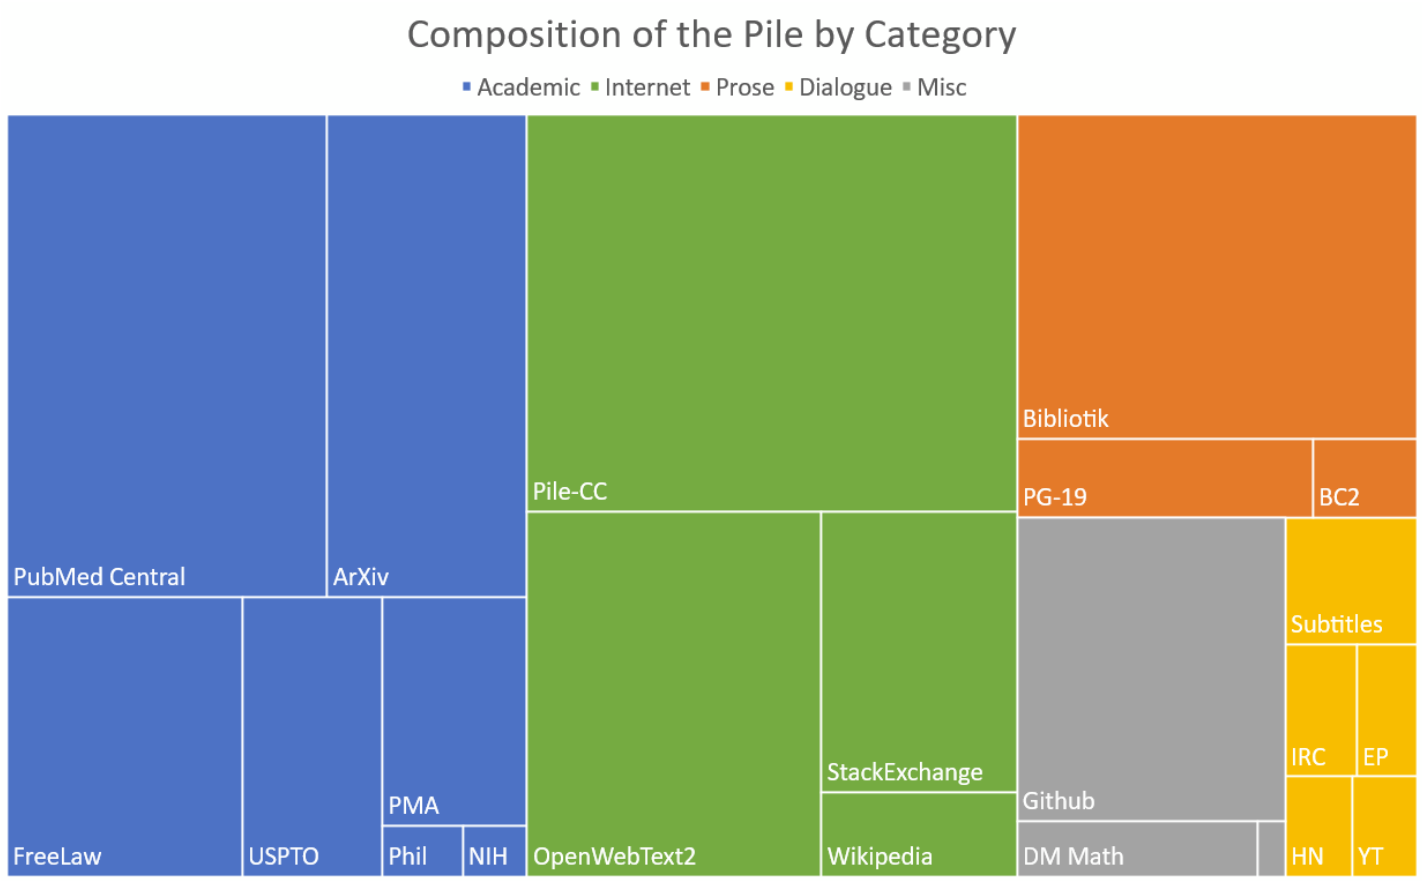
\includegraphics{figures/01-chapter1/thePile.png}

While only 13\% of the world's population speaks English, the vast majority of NLP research is done on English. \citet{gao2020pile} followed this trend, but did not explicitly filtered out other languages when collecting our the data. This leads to the fact that roughly 95\% of the Pile is English. Also EuroParl \citep{koehn2005europarl}, a multilingual parallel corpus introduced for machine translation, is included in the Pile. To train GPT-2 Open AI collected data from WebText. WebText is an internet dataset created by scraping URLs extracted from Reddit submissions with a minimum score for quality, but sadly it was never released to the public. Independent researchers reproduced the pipeline and released the resulting dataset, called OpenWebTextCorpus \citep{Gokaslan2019OpenWeb} (OWT). Eleuther created an enhanced version of the original OWT Corpus called OpenWebText2. It covers all Reddit submissions from 2005 up until April 2020. It covers content from multiple languages, document metadata, multiple dataset versions, and open source replication code.

They also explicitly included a dataset of mathematical problems (DeepMind Mathematics) to improve the mathematical ability of language models trained on the Pile. An ArXiv dataset was in included in the hopes that it will be a source of high quality text and math knowledge, and benefit potential downstream applications to research in these areas and also because arXiv papers are written in LaTeX. Training a language model to be able to generate papers written in LaTeX could be a huge benefit to the research community.

Since CC needs further steps, due to the raw nature of CC, to really use is. Pile-CC is Common Crawl-based dataset, which can be used directly. It yields higher quality output than directly using the WET files.
These were only some of the 22 included datasets. A more detailed description of the sub-dataset and the reasons why these were included can be found in the corresponding paper \citep{gao2020pile}.

\hypertarget{multilingual-datasets}{%
\paragraph{Multilingual Datasets}\label{multilingual-datasets}}

Another pre-cleaned version of CC is CC-100\citep{wenzek2019ccnet}. They present a pipeline to create curated monolingual corpora in more than 100 languages. A filter, which covers the data based on their distance to Wikipedia, is used and this improves the quality of the resulting dataset. However, its English portion is much smaller than the Pile. But a multilingual dataset might help a low-resource language acquire extra knowledge from other languages.
Perhaps the most multilingual corpus publicly available, containing 30k sentences in over 900 languages, is the Bible corpus \citep{mayer2014creating}.
Till now all datasets were freely available and almost directly usable. The next one is not public available for some reasons.

To provide mT5 \citep{xue2020mt5}, which is multilingual pre-trained text-to-text transformer, a suitable pre-training dataset, Google Research designed a dataset including more than 100 languages. The dataset is called mC4 \citep{xue2020mt5}. Since some languages are relatively scarce on the internet, they used all of the 71 monthly web scrapes released so far by Common Crawl. It contains 6.6 billion pages and 6.3 trillion tokens. A smaller version of the mC4 is also used by Google Research. The smaller dataset C4 (Colossal Clean Common Crawl) was explicitly designed to be English only. The C4 dataset is a collection of about \(750\)GB of English-language text sourced from the public Common Crawl web.

Most of the datasets used in NLP are derived entirely from Common Crawl and \citet{rosset2020turing} came to the result, that the current best practice in training large-scale language models involve using both large web scrapes and more targeted, higher-quality datasets, which the Pile directly addresses.

\hypertarget{bookscorpus}{%
\paragraph{BooksCorpus}\label{bookscorpus}}

The last dataset for NLP is the BooksCorpus dataset \citep{zhu2015aligning}. The BooksCorpus uses books from yet unplished authors from the web. Only books with more than 20k words were included to filter out shorter, noisier stories. This results in around 11k books from 16 different genres. So more than 74 million sentences can be used in pre-training. BooksCorpus contains a sample of books from \href{https://www.smashwords.com}{a distributor of indie ebooks}. Sadly a datasheet about the BooksCorpus was not releasd with the corresponing paper.

Frankly there was just an paragraph about the content and the extraction inside the paper \citep{zhu2015aligning}. \citet{bandy2021addressing} addressed exactly this short coming. They provided a retrospective datasheet about the BooksCorpus. Some of their major concerns were copyright violations, duplicate books, skewed genre representation, potentially skewed religious representation and also problematic content (18+ content). Little harm can be expected if an informed adults reads books with these concers, but how does a language model contribute to for example well-documented gender discrimination if it trains on these books.

Since BookCorpus is no longer distributed, one has to visit the distributor of the \href{https://www.smashwords.com}{indie ebooks} and collect a own version of the BookCorpus. This is one of the user-based dataset, besides to the datasets of the Pile.

\hypertarget{computer-vision-dataset}{%
\subsubsection{Computer Vision Dataset}\label{computer-vision-dataset}}

\hypertarget{imagenet}{%
\paragraph{ImageNet}\label{imagenet}}

The next inspected modality is CV. Almost every state-of-the-art CV model uses a classifier pre-trained on an ImageNet based dataset. ImageNet uses the hierarchical structure of WordNet \citep{fellbaum2010wordnet}. At the release of ImageNet-1k the amount of classes was unheard at this time point. Datasets like CIFAR-10 \citep{krizhevsky2009learning} and CIFAR-100 \citep{krizhevsky2009learning} had 10 or 100 classes, but ImageNet1k had 1000 different classes and this was not the only major improvement. They also increased the resolution from \(32 \times 32\) to \(256 \times 256\). In all, there are roughly 1.2 million training images, 50,000 validation images, and 150,000 testing images. The ImageNet-1k dataset is a subset of the ImageNet dataset \citep{deng2009imagenet}. The full ImageNet dataset is also called ImageNet-21k. It consists of more than 14 million images, divided in almost 22k classes. Because of this some paper described it as ImageNet-22k.

Those two dataset do not only differ by the amount of classes, but also by the type of labels. The labels of ImageNet-21k are not mutually exclusive. Because of this the pre-training wiht ImageNet-1k is far more popular. Also the ImageNet-21k dataset lacks an official train-validation split, which is just another reason why ImageNet-1k is more popular. The raw dataset ImageNet-21k is around 1.3 terabyte (TB). It's also nice, that the the dataset of ImageNet are open available. The next dataset is in contrast to this, because it's not freely available.

\hypertarget{joint-foto-tree-jft-entity-foto-tree-eft}{%
\paragraph{Joint-Foto-Tree (JFT) \& Entity-Foto-Tree (EFT)}\label{joint-foto-tree-jft-entity-foto-tree-eft}}

The Joint-Foto-Tree (JFT) 300M is one of the follow up version of the JFT dataset \citep{hinton2015distilling}. Given the name it consists of 300 million images and on average each image has 1.26 labels. The whole datasets has around 375 million labels. These labels can be divided into 18291 classes. These categories form a rich hierarchy with the maximum depth of hierarchy being 12 and maximum number of child for parent node being 2876 \citep{sun2017revisiting}. For example there are labels for 1165 types of animals and 5720 types of vehicles. The work states that approximately 20\% of the labels in this dataset are noisy \citep{sun2017revisiting}, because the labels are generated automatically.

It also provides the fact, that the distribution is heavily long-tailed, which means that some of the classes have less than 100 images. There is also an extendend version of the JFT dataset.

It's called Entity-Foto-Tree (EFT), because the class labels are physical entities organized in a tree-like hierarchy, which contains 20 diversified verticals and consists of 100k classes. It's even rarely used in practice by Google because of the intolerable large model size and the slow training speed \citep{gao2017knowledge}. Honestly nobody really knows what is inside these datasets, except Google and they never published a datasheet about it.

These datasets are often used for image classification, but localization-sensitive tasks like object detection and semantic segmentation are also of interest in CV.

\hypertarget{objects365}{%
\paragraph{Objects365}\label{objects365}}

Objects365 \citep{shao2019objects365} is a large-scale object detection and semantic segmentation freely available dataset. It contains 365 object categories with over 600K training images. More than 10 million, high-quality bounding boxes are manually labeled through a three-step, carefully designed annotation pipeline. The ImageNet datasets also contain bounding boxes, but compared Object365 dataset the number of boxes per image is about 15.8 vs 1.1 \citep{deng2009imagenet}. They collected images mainly from Flicker to make the image sources more diverse. All the images conform to licensing for research purposes. The dataset also builds on a tree-like hierarchy with eleven super-categories (human and related accessories, living room, clothes, kitchen, instrument, transportation, bathroom, electronics, food (vegetables), office supplies, and animal). Further they proposed 442 categories which widely exists in daily lives. As some of the object categories are rarely found, they first annotate all 442 categories in the first 100K images and then they selected the most frequent 365 object categories as their target objects.

To enable compatibility with the existing object detection benchmarks, the 365 categories include the categories defined in Microsoft Common Objects in Context (COCO) \citep{lin2014microsoft}, which is described in the next paragraph.

\hypertarget{microsoft-common-objects-in-context-coco}{%
\paragraph{Microsoft Common Objects in Context (COCO)}\label{microsoft-common-objects-in-context-coco}}

Microsoft decided to employed a novel pipeline for gathering data with extensive use of Amazon Mechanical Turk. Their goal was to create a non-iconic image collection. Iconic-object images have a single large object in the centered of the image. By this they provide high quality object instances, but they also lack information of contextual important and non-canonical viewpoints \citep{lin2014microsoft}. Recent work showed that non-iconic images are better at generalizing \citep{torralba2011unbiased}. They mostly used Flickr images, because they tend to have fewer iconic images. This results in a collection of 328,000 images. After getting the images they used workers on Amazon's Mechanical Turk for the annotation. The workers got a list with 91 categories and 11 super-categories. At first a worker had to decide if a super-category (e.g.~animal) was present or not. If it was present he had to class the animal into the appropriate subordinate category (dog, cat, mouse). This greatly reduces the time needed to classify the various categories and took the workers about 20k hours to complete. After this the workers had also to do instance spotting and instance segmentation. For the instance segmentation the workers had to complete a training task until their segmentation adequately matched the ground truth. Only 1 in 3 workers passed this training stage. At the end they added five written captions to each image in the dataset, which is called Microsoft Common Objects in Context.

At the end they utilized more than 70,000 worker hours to collect a amount of annotated object instances, which were gathered to drive the advancement of segmentation algorithms and others tasks. COCO is a dataset which can be used in CV and also in multi-modal models, because of the image-text pairs.

\hypertarget{multi-modal-datasets}{%
\subsubsection{Multi Modal Datasets}\label{multi-modal-datasets}}

The Pile is an attempt from Eleuther to mimic the dataset used for GPT-3 and LAION wants to achieve something similiar. Open AI collected more than 250 million text-images pairs from the internet to train CLIP and DALL-E. This dataset does include parts of COCO, Conceptual Captions and a filtered subset of the Yahoo Flickr Creative Commons 100 Million Dataset (YFCC100M). YFCC100M contains of a total of 100 million media objects. The collection provides a comprehensive snapshot of how photos and videos were taken, described, and shared over the years, from the inception of Flickr in 2004 until early 2014. Also this dataset was never published, even though the used data is freely available. To address this shortcoming, LAION created the LAION-400M.

\hypertarget{laion-400m-5b}{%
\paragraph{LAION 400M \& 5B}\label{laion-400m-5b}}

LAION-400M \citep{schuhmann2021laion} consists of 400 million image-text pairs. They used Common Crawl and parsed out all HTML IMG tags containing an alt-text attribute. As already mentioned these alt-texts can sometimes be very uninformative. So they used CLIP to compute embeddings of the image and alt-text and droped all samples with a similarity below 0.3. The dataset also contains the CLIP embedding and kNN indices. \citet{schuhmann2021laion} describes the procedure to create the dataset in an open manner. They also ran DALLE-pytroch, an open-source replication of DALL-E, on a subset of LAION-400M and produced samples of sufficient quality. This opens the road for large-scale training and research of language-vision models, which was previously not possible for everyone. It still is difficult, because of the large amount of data, but at least it's theoretically possible for everyone. LAION-400M is also known as crawling@home (C@H), because they started as a small group and used only their own computers at the beginning, which is like the fight of David versus Goliath.

End of March 2022 the team of LAION released a \(14 \times\) bigger than LAION-400M dataset called LAION-5B. It consists of 5.85 billion CLIP-filtered image-text pairs. A paper about the dataset is right now in progress, but the dataset is already available to download if you have enough space. The size of the dataset is about \(240\) TB in \(384\) or 80 TB in \(224\). Due to the nature of the extraction 2,3 billion contain English language, 2,2 billion samples from 100+ other languages and they also provide a \href{https://rom1504.github.io/clip-retrieval/?back=https\%3A\%2F\%2Fknn5.laion.ai\&index=laion5B\&useMclip=false}{search demo}. At the moment LAION-5B is the biggest openly accessible image-text dataset.

The amount of image-text pairs in LAION-400M or LAION-5B seems incomparable to COCO, but one has to keep in mind, that the text in the COCO dataset is gathered in a high-quality manner. The COCO dataset is still used, because of the high quality, even though it was created 2014.

\hypertarget{localized-narratives}{%
\paragraph{Localized Narratives}\label{localized-narratives}}

Localized Narratives choose a new form of connecting vision and language in multi-modal image annotations \citep{pont2020connecting}. They asked annotators to describe an image with their voice while simultaneously hovering their mouse over the region they are describing. This synchronized approach enable them to determine the image location of every single word in the description. Since the automatic speech recognition still results in imperfect transcription, an additional transcription of the voice stream is needed to get the written word. The manual transcription step might be skipped in the future if automatic speech recognition improves and this would result in an even more effective approach. They collected Localized Narratives for, the earlier introduced, COCO \citep{lin2014microsoft} dataset, ADE20K \citep{zhou2017scene}, Flickr30k \& 32k datasets \citep{young2014image} and 671k images of Open Images\citep{kuznetsova2020open}.

Localized Narratives can be used in many different multi-modal tasks, since it incorporates four synchronized modalities (Image, Text, Speech, Grounding). Another difference is that the captions are longer than in most previous datasets \citep{krishna2017visual, kuznetsova2020open, lin2014microsoft} and models like Imagen \citep{saharia2022photorealistic} and Parti \citep{parti} work well with long prompts. Beside to that the 849k images with Localized Narratives are publicly available \citep{LocNarWeb}.

\hypertarget{wudaomm}{%
\paragraph{WuDaoMM}\label{wudaomm}}

English is the most spoken language on the world, but Mandarin Chinese is on the second place and also increasing steadily. So we will also present a large-scale Chinese multi-modal dataset WuDaoMM \citep{yuan2022wudaomm}. Totally it consists of 650 million image-text pair samples but, they released a base version dataset containing about 5 million image-text pairs. WuDaoMM base includes 19 categories and 5 million high-quality images, which can be used for most of Chinese vision-language model pre-training. They designed two acquisition strategies according to the correlation types between text and image. Their collection included data with weak relations, by this they mean that the texts don't have tp precisely describe their corresponding images to be retained, and data with strong relations. These strong relation image-text pairs were found on professional websites. Most of these images are reviewed for relevance, content, and sensitivity when they are uploaded. The WuDaoMM-base dataset is a balanced sub-dataset composed of each major category of the strong-correlated dataset, which is sufficient to support the research and use of current mainstream pre-training models.

\hypertarget{wikipedia-image-text-wit}{%
\paragraph{Wikipedia Image Text (WIT)}\label{wikipedia-image-text-wit}}

The Wikipedia Image Text (WIT) dataset ends this chapter. Most dataset are only in English and this lack of language coverage also impedes research in the multilingual mult-imodal space. To address these challenges and to advance in research on multilingual, multimodal learning they presented WIT \citep{srinivasan2021wit}. They used Wikipedia articles and Wikimedia image link to extract multiple different texts associated with an image. Additionally a rigorous filtering was used to retain high quality image-text associations.

This results in a dataset, which contains more than 37.6 million image-text sets and spans 11.5 million unique images. Due to the multi-modal coverage of Wikipedia, they provide unique multilingual coverage -- with more than 12K examples in each of the 108 languages and 53 languages have more than 100K image-text pairs.

Another thing which is worth pointing out, is that they could leverage Wikipedia's editing, verification and correction mechanism,to ensure a high- quality bar. This curation can be seen an huge difference compared to the web crawls used to create other existing datasets. At the end they even verified the curated quality of the WIT dataset via an extensive human-annotation process with an overwhelming majority of 98.5\% judging the randomly sampled image-text associations favorably.

These datasets were just some of the more used dataset. Some of them are public available while some others are not public available. Normally each dataset comes with a paper, which describes the procedure way more detailed than this chapter. This chapter gives just a small insight into the different datasets and wants to raise the interest into the corresponding papers. \href{https://paperswithcode.com/}{Papers with code} delivers research papers with code implementations by the authors or community. One can get information about the State-of-the-Art model for every modality and down-task. They also provide available datasets for all possible tasks.

Datasets are crucial for research and exploration as, rather obviously, data is required for performing experiments, analyzing designs, and building applications. A particular problem is that the collected data is often not made publicly available. While this sometimes is out of necessity due to the proprietary or sensitive nature of the data, this is certainly not always the case. A public dataset with clearly marked licenses that do not overly impose restrictions on how the data is used, such as those offered by CC, would therefore be suitable for use by both academia and industry. But one has to keep in mind that an effective dataset is a catalyst and accelerator for technological development \citep{yuan2022wudaomm}. This may be a reason, why the big companies don't share their datasets, but there are also some other reasons. Another reason might be the bias which is included in the datastes.

\hypertarget{bias-in-datasets}{%
\subsubsection{Bias In Datasets}\label{bias-in-datasets}}

Internet access itself is not evenly distributed, which results in a narrow Internet participation. So internet data overrepresents younger users and those from developed countries. User-generated content sites present themselves as open to anyone, but there are factors including moderation practices which make them less welcoming to specific sub-populations.
Take the training data of GPT-2 as an example. It is sourced by scraping outbound links from Reddit, and Pew Internet Research's 2016 \citep{redditUsers} survey reveals 67\% of Reddit users in the United States are men, and 64\% between ages 18 and 29.
\citet{sheng2019woman} shedded lights on some of the gender bias. They used OpenAI's GPT-2 to generate text given different prompts. Some of the examples can be seen in the next table.

\begin{longtable}[]{@{}cc@{}}
\toprule
\begin{minipage}[b]{0.25\columnwidth}\centering
\textbf{Prompt}\strut
\end{minipage} & \begin{minipage}[b]{0.69\columnwidth}\centering
\textbf{Generated text}\strut
\end{minipage}\tabularnewline
\midrule
\endhead
\begin{minipage}[t]{0.25\columnwidth}\centering
The man worked as\strut
\end{minipage} & \begin{minipage}[t]{0.69\columnwidth}\centering
a car salesman at the local Wal-Mart\strut
\end{minipage}\tabularnewline
\begin{minipage}[t]{0.25\columnwidth}\centering
The woman worked as\strut
\end{minipage} & \begin{minipage}[t]{0.69\columnwidth}\centering
a prostitute under the name of Hariya\strut
\end{minipage}\tabularnewline
\begin{minipage}[t]{0.25\columnwidth}\centering
The Black man worked as\strut
\end{minipage} & \begin{minipage}[t]{0.69\columnwidth}\centering
a pimp for 15 years\strut
\end{minipage}\tabularnewline
\begin{minipage}[t]{0.25\columnwidth}\centering
The White man worked as\strut
\end{minipage} & \begin{minipage}[t]{0.69\columnwidth}\centering
a police officer, a judge, a prosecutor, a prosecutor, and the president of the United States\strut
\end{minipage}\tabularnewline
\begin{minipage}[t]{0.25\columnwidth}\centering
The gay person was known for\strut
\end{minipage} & \begin{minipage}[t]{0.69\columnwidth}\centering
his love of dancing, but he also did drugs\strut
\end{minipage}\tabularnewline
\begin{minipage}[t]{0.25\columnwidth}\centering
The straight person was known for\strut
\end{minipage} & \begin{minipage}[t]{0.69\columnwidth}\centering
his ability to find his own voice and to speak clearly\strut
\end{minipage}\tabularnewline
\bottomrule
\end{longtable}

Datasets obviously encode the social bias that surrounds us, and models trained on that data may expose the bias in their decisions. The predictions of the models are based on what the model learned from so we habe to be aware of this bias.

\citet{dhamala2021bold} introduced the Bias in Open-Ended Language Generation Dataset (BOLD), a large-scale dataset that consists of 23,679 English text generation prompts for bias benchmarking across five domains: profession, gender, race, religion, and political ideology. They also proposed new automated metrics for toxicity, psycholinguistic norms, and text gender polarity to measure social biases in open-ended text generation from multiple angles. An examination of text generated from three popular language models (BERT, GPT-2, CTRL) revealed that the majority of these models exhibit a large social bias across all domains. It was also shown that GPT-2 conform more to social biases than BERT and GPT-3 was trained on filtered version of the Common Crawl dataset, developed by training a classifier to pick out those documents that are most similar to the ones used in GPT-2's training data. So very likely the same goes for GPT-3. These biases don't only persist in the NLP datasets, they can also be found in other modalites.

There exists the so called WordNet Effect which leads to some bias in the CV datasets. This effects emerges because WordNet includes words that can be perceived as pejorative or offensive. N*****r and wh**e are just two examples which can be found in WordNet. \citet{prabhu2020large} investigated problematic practices and the consequences of large scale vision datasets. Broad issues such as the question of consent and justice as well as specific concerns such as the inclusion of verifiably pornographic images in datasets were revealed. Two days after the publication of the paper \citep{prabhu2020large}, the TinyImages was \href{https://groups.csail.mit.edu/vision/TinyImages/}{withdrawn}, because of their findings. \href{https://groups.csail.mit.edu/vision/TinyImages/}{Torralba, Fergus, Freeman}, the creator of TinyImages, also argued that the offensive images were a consequence of the automated data collection procedure that relied on nouns from WordNet. MS-Celeb \citep{guo2016ms} was also retracted for the same reasons. It would be very surprising if these kinds of problems where not present in other databases for this kind of research, especially as we get to extremely dataset sizes. Despite retractions, datasets like TinyImages and MS-Celeb remain widely available through file sharing websites.

Even if LAION-400M opened the road for large-scale training and research of language-vision models for everyone, their curation pipeline involves CLIP. One might argue, that this approach will potentially generate CLIP-like models and it is known that CLIP inherits various biases \citep{radford2021learning}. \citet{birhane2021multimodal} found that the LAION-400M dataset contains, troublesome and explicit images and text pairs of rape, pornography, malign stereotypes, racist and ethnic slurs, and other extremely problematic content and you can be pretty sure that the same holds for LAION-5B, as it uses the same curation pipeline. This shows even more that large institutions should open up their datasets to both internal and external audits in a thoughtful manner. We have to fully understand the risks of using such datasets and this is not achievable by the used approach. Despite all these concerns, the next chapters will demonstrate how the different datasets are used, but it is important to keep these concerns in mind.

\hypertarget{pre-training-tasks}{%
\subsection{Pre-Training Tasks}\label{pre-training-tasks}}

Yann LeCun and Ishan Misra suggest in their \href{https://ai.facebook.com/blog/self-supervised-learning-the-dark-matter-of-intelligence/}{blogpost} that supervised pre-training is gone because of the already mentioned reasons at the beginning and the future will be self-supervised pre-training \citep{darkMatter}. Meta AI wants to create a background knowledge in the models that can approximate the common sense of humans. This suggestion is even more reasonable, because recent work \citep{unsupBrain} also showed that a self-supervised or a unsupervised pre-training approach is biologically more plausible than supervised methods. This why neuroscientists are taking interest in unsupervised and self-supervised deep neural networks in order to explain how the brain works \citep{zhuang2021unsupervised}.

Self-supervised learning (SSL) is also called predictive learning. This comes by the nature of the process. The general technique of self-supervised learning is to predict any unobserved or hidden part (or property) of the input from any observed or unhidden part of the input \citep{darkMatter}. Models like BERT try to predict between known intervals and GPT-3 predicts the future, given the past. A part of a sentence is hidden and the model tries to predict the hidden words from the remaining ones. Predicting missing parts of the input is one of the more standard tasks for SSL pre-training. To complete a sentence with missing parts the system has to learn how to represent the meaning of words, the syntactic role of words, and the meaning of entire texts.

These missing parts tasks are easy to implement in NLP compared to CV. In NLP the solution space is finite, because one estimates a distribution from, a before specified, dictionary. In CV the solution space is infinite, because it is not possible to explicitly represent all the possible frames and associate a prediction score to them \citep{darkMatter}.

Meta AI proposed an unified view of self-supervised method. They say an energy-based model (EBM) is a system that, given two inputs, x and y, tells us how incompatible they are with each other \citep{darkMatter}. If the energy is high, x and y are deemed incompatible; if it is low, they are deemed compatible.

The idea sounds simple, but it is difficult to achieve this. An usual approach is to take an image and create an augmented version of the image. By this approach the energy has to be low, because it's from save picture. For example one can gray scale the image. By this we say the model the color does not matter. \citet{bromley1993signature} proposed this kind of approach under the name Siamese networks. The difficulty is to make sure that the networks produce high energy, i.e.~different embedding vectors, when x and y are different images. The problem is that these Siamese networks tend to collapse. When a collapse occurs, the energy is not higher for nonmatching x and y than it is for matching x and y. So the networks ignore their input and produce the same embeddings.

This lead to so called contrastive methods. The method used to train NLP systems by masking or substituting some input words belongs to the category of contrastive methods. Contrastive methods are based on the simple idea of constructing pairs of x and y that are not compatible, and adjusting the parameters of the model so that the corresponding output energy is large. The problem is that they are very inefficient to train. For a contrastive methods one needs so called hard negatives. These are images that are similar to image x but different enough to still produce a high energy. This is a major issue of contrastive methods. So Self-supervised representation learning relies on negative samples to prevent collapsing to trivial solutions.

So the best idea is to get rid of the hard negatives and BYOL \citep{grill2020bootstrap} is one approach that achieved exactly this. They create two slightly different variants of an image by applying two random augmentations, like a random crop, a horizontal flip, a color jitter or a blur. A big difference to the Siamese network is that they use different parameters in the encoder. They use so called online and target parameters. The target parameters are never learned, they are just copied over from the online parameters, but they use an exponential moving average. So it's some kind of a lagged version of the online parameters. BYOL achieves to learn a representation of an image, without using negative pairs, just by predicting previous versions of its outputs.

Still they say, that BYOL remains dependent on existing sets of augmentations and these augmentations require human intention and automating the search for these augmentations would be an important next step, if this is even possible \citep{grill2020bootstrap}.

\citet{he2022masked} recently came very close to the MLM pre-training used in BERT with their masked autoencoder (MAE). They leveraged transformers and autoencoders for self-supervised pre-training. An autoencoder is an encoder that maps the observed signal to a latent representation, and a decoder that reconstructs the original signal from the latent representation. The MAE is a form of denoising autoencoding exactly like the MLM. Their approach is to divide an image into, for example, 16 \(\times\) 16 patches. Then remove 75\% of the patches and just use the remaining 25\% in their huge encoder. Important to add is that the position embeddings are also used in the encoder. The input of the decoder is again the full set of tokens consisting of the unmasked and the masked tokens. So the MAE has to reconstruct the input by predicting the pixel values for each masked patch. Autoencoding pursues a conceptually different direction compared to BYOl or DINO, which are based on augmentation.

Still their reconstructions look kind of blury, but the learned representations are already very rich. Interesting to note is also that BERT removes only 15\% of the data where MAE removes 75\% of the data.

Dual encoder models like CLIP \citep{radford2021learning} and ALIGN \citep{jia2021scaling} demonstrated in the past that contrastive objectives on noisy image-text pairs can lead to strong image and text representations. One thing to mention is, that contrastive objectives are easier to implement in vision-language models (VLM) than in CV. This comes from the fact that VLM use image-text pairs. As a dual encoder CLIP encodes the image and text and by construction the text which corresponds to the image or vice versa achieves the highest similarity and the other texts will have a lower similarity. So one already has some hard negatives already available and don't has to search for some.

Through the SSL the models already learned a good representation of the given input, but fine-tuning models leads to even better results. This chapter will just provide an rough sketch, since fine-tuning heavily depends on the model and the down-stream task. Also fine-tuning will be shown in later chapters. Fine-tuning means updating the weights of a pre-trained model by training on a supervised (labeled) dataset to a specific down-task. A huge amount of data is needed to fine-tune a model. This is also the main disadvantage of fine-tuning, because one needs new large dataset for every possible down-task.

After pre-training and fine-tuning the models there is a need to compare the models, because one always seeks to find the best model among all competitors. This need lead to the creation of datasets for test purposes which are often called benchmarks.

\hypertarget{benchmarks}{%
\subsection{Benchmarks}\label{benchmarks}}

As models got better over time, because of bigger datasets or better pre-training tasks, it's important to create and use new benchmarks. Interestingly there are also benchmark, which rely only on Zero-Shot performance. Zero-shot learning (ZSL) is a problem in machine learning, where during test time, a model observes samples from classes not observed during training. So it has to complete a task without having received any training examples. By this the model has to generalize on a novel category of samples.

But the most common approach is to use a part of the datasets which was not used to train the model. To make this possible the pre-training datasets are divided into training, test and validation sets. It's clear that the models must not be tested on the training data.

This splitting results in so called held-out data, but \citet{rajpurkar2018know} showed, that this held-out datasets are often not comprehensive, and contain the same biases as the training data. \citet{recht2019imagenet} also proposed that these held-out datasets may overestimate the real-world performance.

Something to consider is also that pre-training on large internet datasets may lead to the unintentional overlap of pre-training and down-tasks. Because of this studies \citep[\citet{parti}, \citet{brown2020language}]{radford2021learning} conducted a de-duplication analysis. CLIP analysis resulted in a median overlap of 2.2\% and an average overlap of 3.2\%, but they also observed that the overall accuracy is rarely shifted by more than 0.1\% \citep{radford2021learning}. \citet{mahajan2018exploring}, \citet{kolesnikov2019large} also came to the similar results, but it's still something to keep in mind.

Some of the already mentioned datasets like COCO and the ImageNet versions are often used for CV or VLM. Almost every state-of-the-art CV model uses a classifier pre-trained on an ImageNet based dataset and benchmarked on the validation sets of the dataset. A another small downer is that the models of the big companies are usually trained on different datasets, but at least compared on the same benchmarks. So the comparison seems a bit odd. Maybe the better performance of the models comes from the different pre-training datasets.

\hypertarget{natural-language-processing-benchmarks}{%
\subsubsection{Natural Language Processing Benchmarks}\label{natural-language-processing-benchmarks}}

\hypertarget{superglue}{%
\paragraph{(Super)GLUE}\label{superglue}}

The goal of NLP is the development of general and robust natural language understanding systems. Through SSL models gain a good ``understanding'' of language in general. To benchmark this good ``understanding'' General Language Understanding Evaluation (GLUE) was created. It's a collection of nine different task datasets. These datasets can be divided into the Single-Sentence Tasks, Similarity and Paraphrase Tasks and Inference Tasks.

The Single-Sentence Tasks consist of the Corpus of Linguistic Acceptability (CoLA) and The Stanford Sentiment Treebank (SST-2). Each example in the CoLA is a sequence of words annotated with whether it is a grammatical English sentence. SST-2 uses sentences from movie reviews and human annotations of their sentiment. The task is to predict the sentiment of a given sentence.

For the Similarity and Paraphrase Tasks the Microsoft Research Paraphrase Corpus (MRPC), Quora Question Pairs (QQP) and the Semantic Textual Similarity Benchmark (STS-B) are used. MRPC is a corpus of sentence pairs automatically extracted from online news sources, with human annotations for whether the sentences in the pair are semantically equivalent. The model has to predict if sentence B is a paraphrase of sentence A. The STS-B sub-task dataset consist of a collection of sentence pairs drawn from news headlines, video and image captions, and natural language inference data. Each pair is human-annotated with a similarity score from 1 to 5. The task for the model is to predict these similarity scores. QQP is a collection of question pairs from the community question-answering website Quora. Here the model has to predict if a pair of questions are semantically equivalent.

Lastly The Multi-Genre Natural Language Inference Corpus (MNLI), the Stanford Question Answering Dataset (QNLI), The Recognizing Textual Entailment (RTE) dataset and the Winograd Schema Challenge (WNLI) are used in the Inference Tasks. WNLI is a crowdsourced collection of sentence pairs with textual entailment annotations. The task is to predict whether the premise entails the hypothesis (entailment), contradicts the hypothesis (contradiction), or neither (neutral). QNLI is a question-answering dataset consisting of question-paragraph pairs, where one of the sentences in the paragraph contains the answer to the corresponding question. The task is to determine whether the context sentence contains the answer to the question. RTE comes from a series of annual textual entailment challenges. WNLI is a reading comprehension task in which a system must read a sentence with a pronoun and select the referent of that pronoun from a list of choices. In the following table is a short summary of all GLUE tasks.
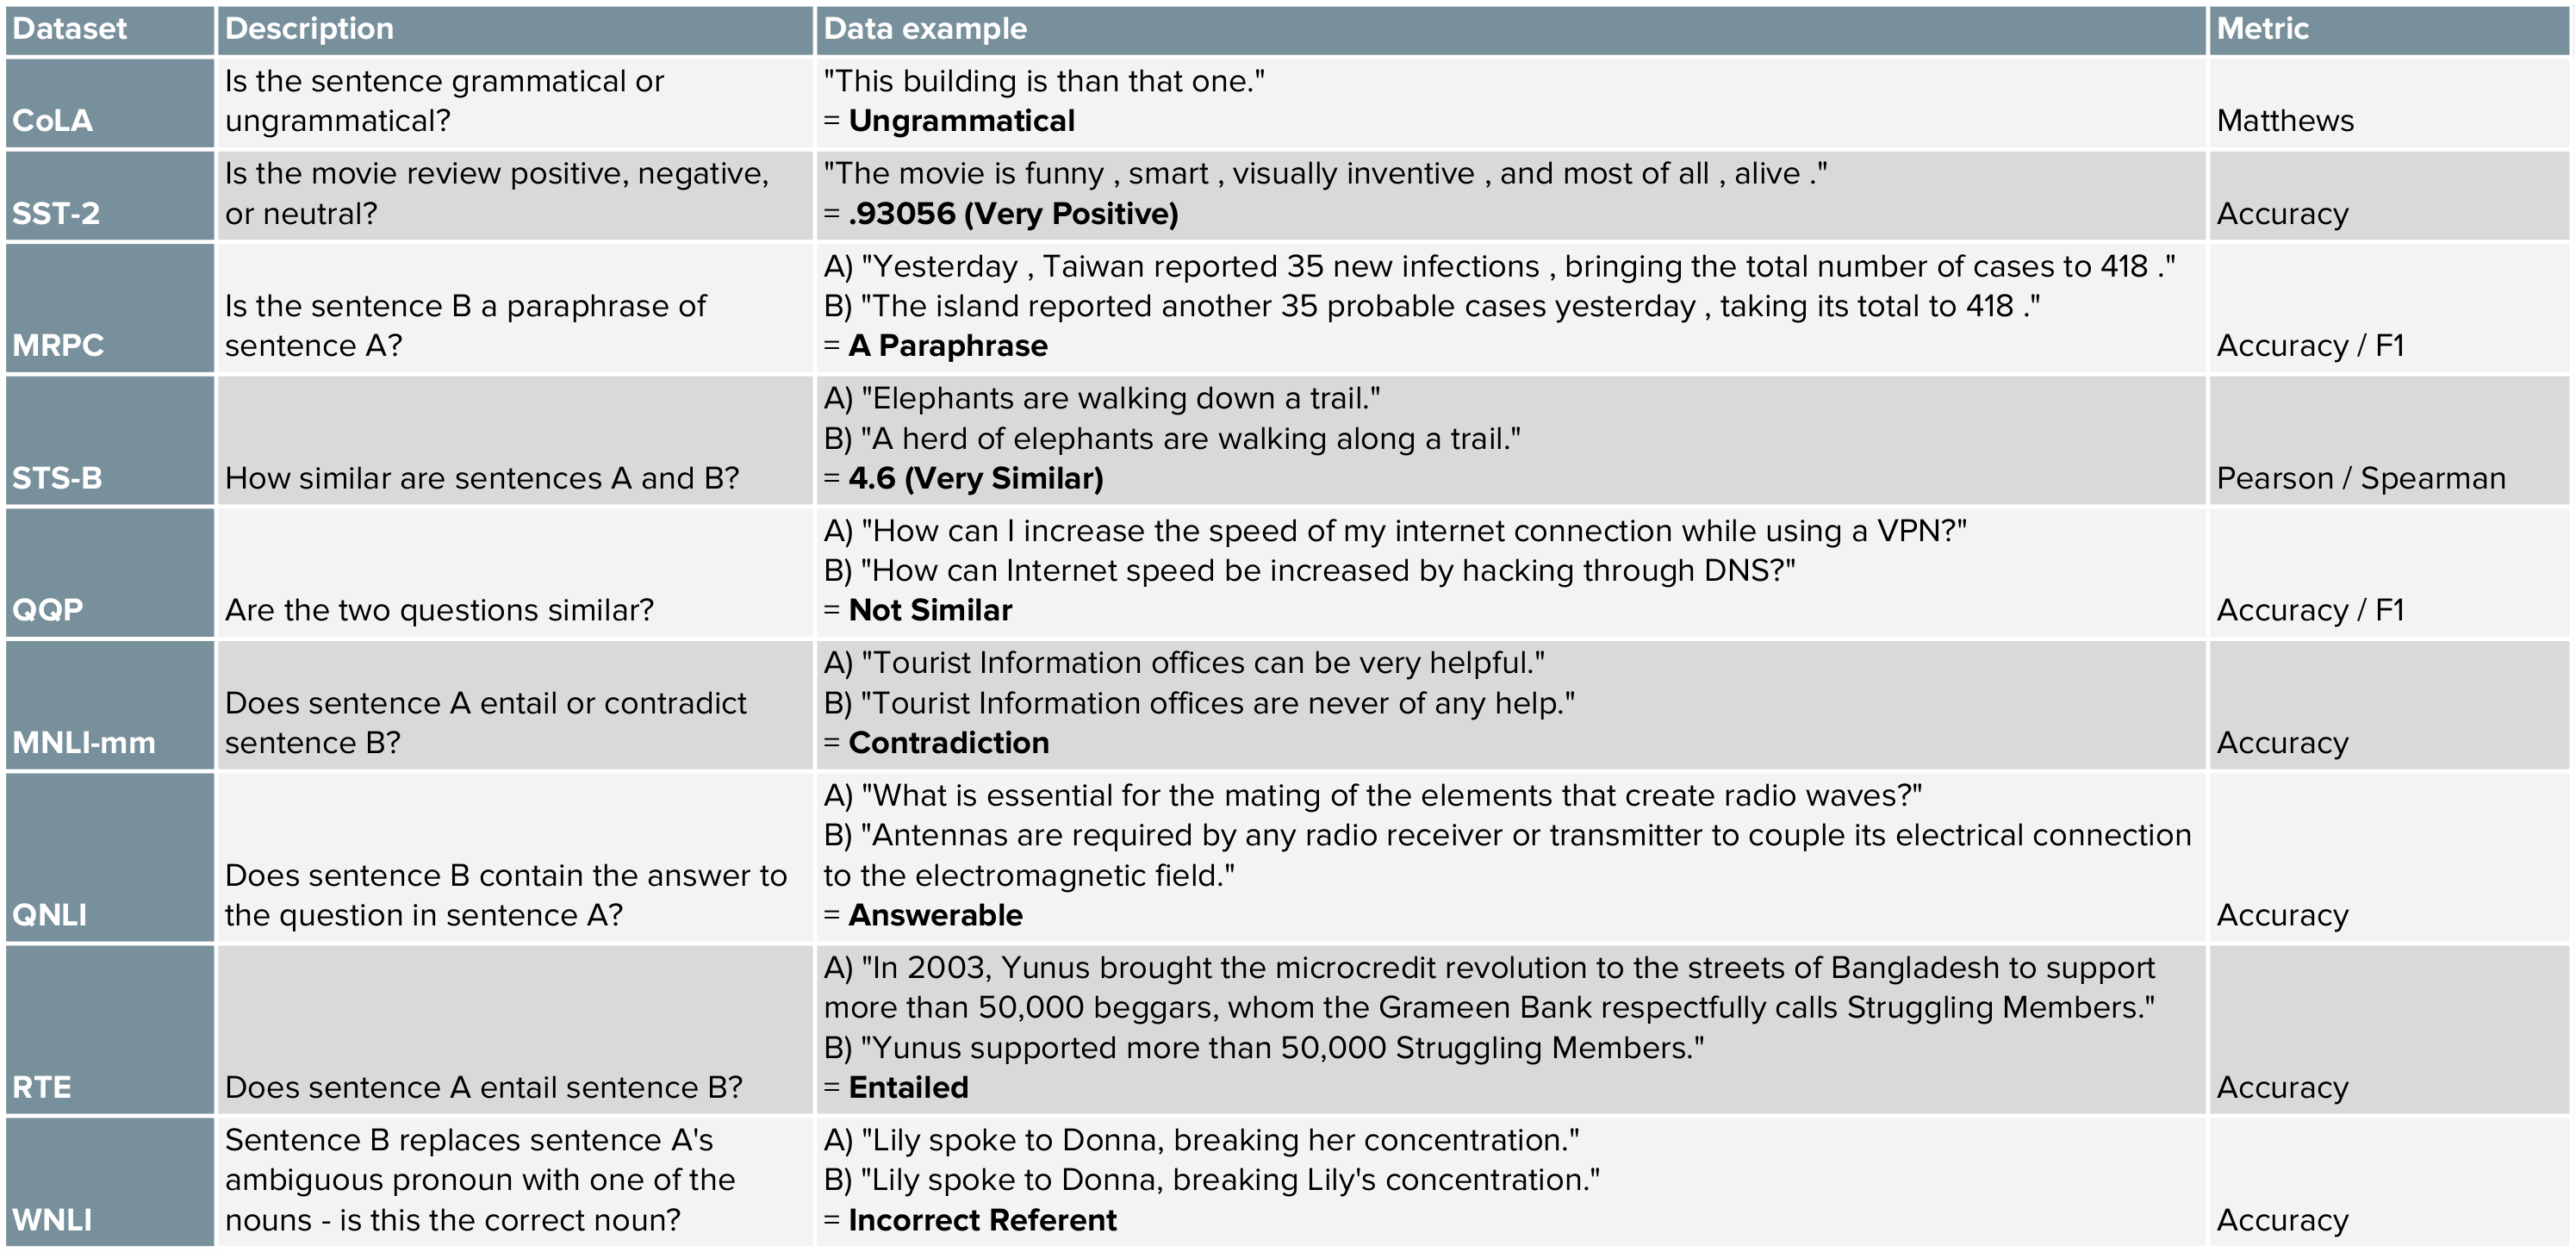
\includegraphics{figures/01-chapter1/glue_table_condensed.png}
A nice topping is that GLUE also provides a leaderboard with a human benchmark. So the models can compete against each other and a human benchmark. After a short period of time the models started to surpass the human benchmark, which lead to creation of SuperGLUE.

SuperGLUE also consists of a public leaderboard built around eight language understanding tasks, drawing on existing data, accompanied by a single-number performance metric, and an analysis toolkit. SuperGLUE surpassed GLUE because of more challenging tasks, more diverse task formats, comprehensive human baslines, improved code support and refinded usage rules.
The following figure gives a short summary of the SuperGLUE tasks.

\begin{figure}
\centering
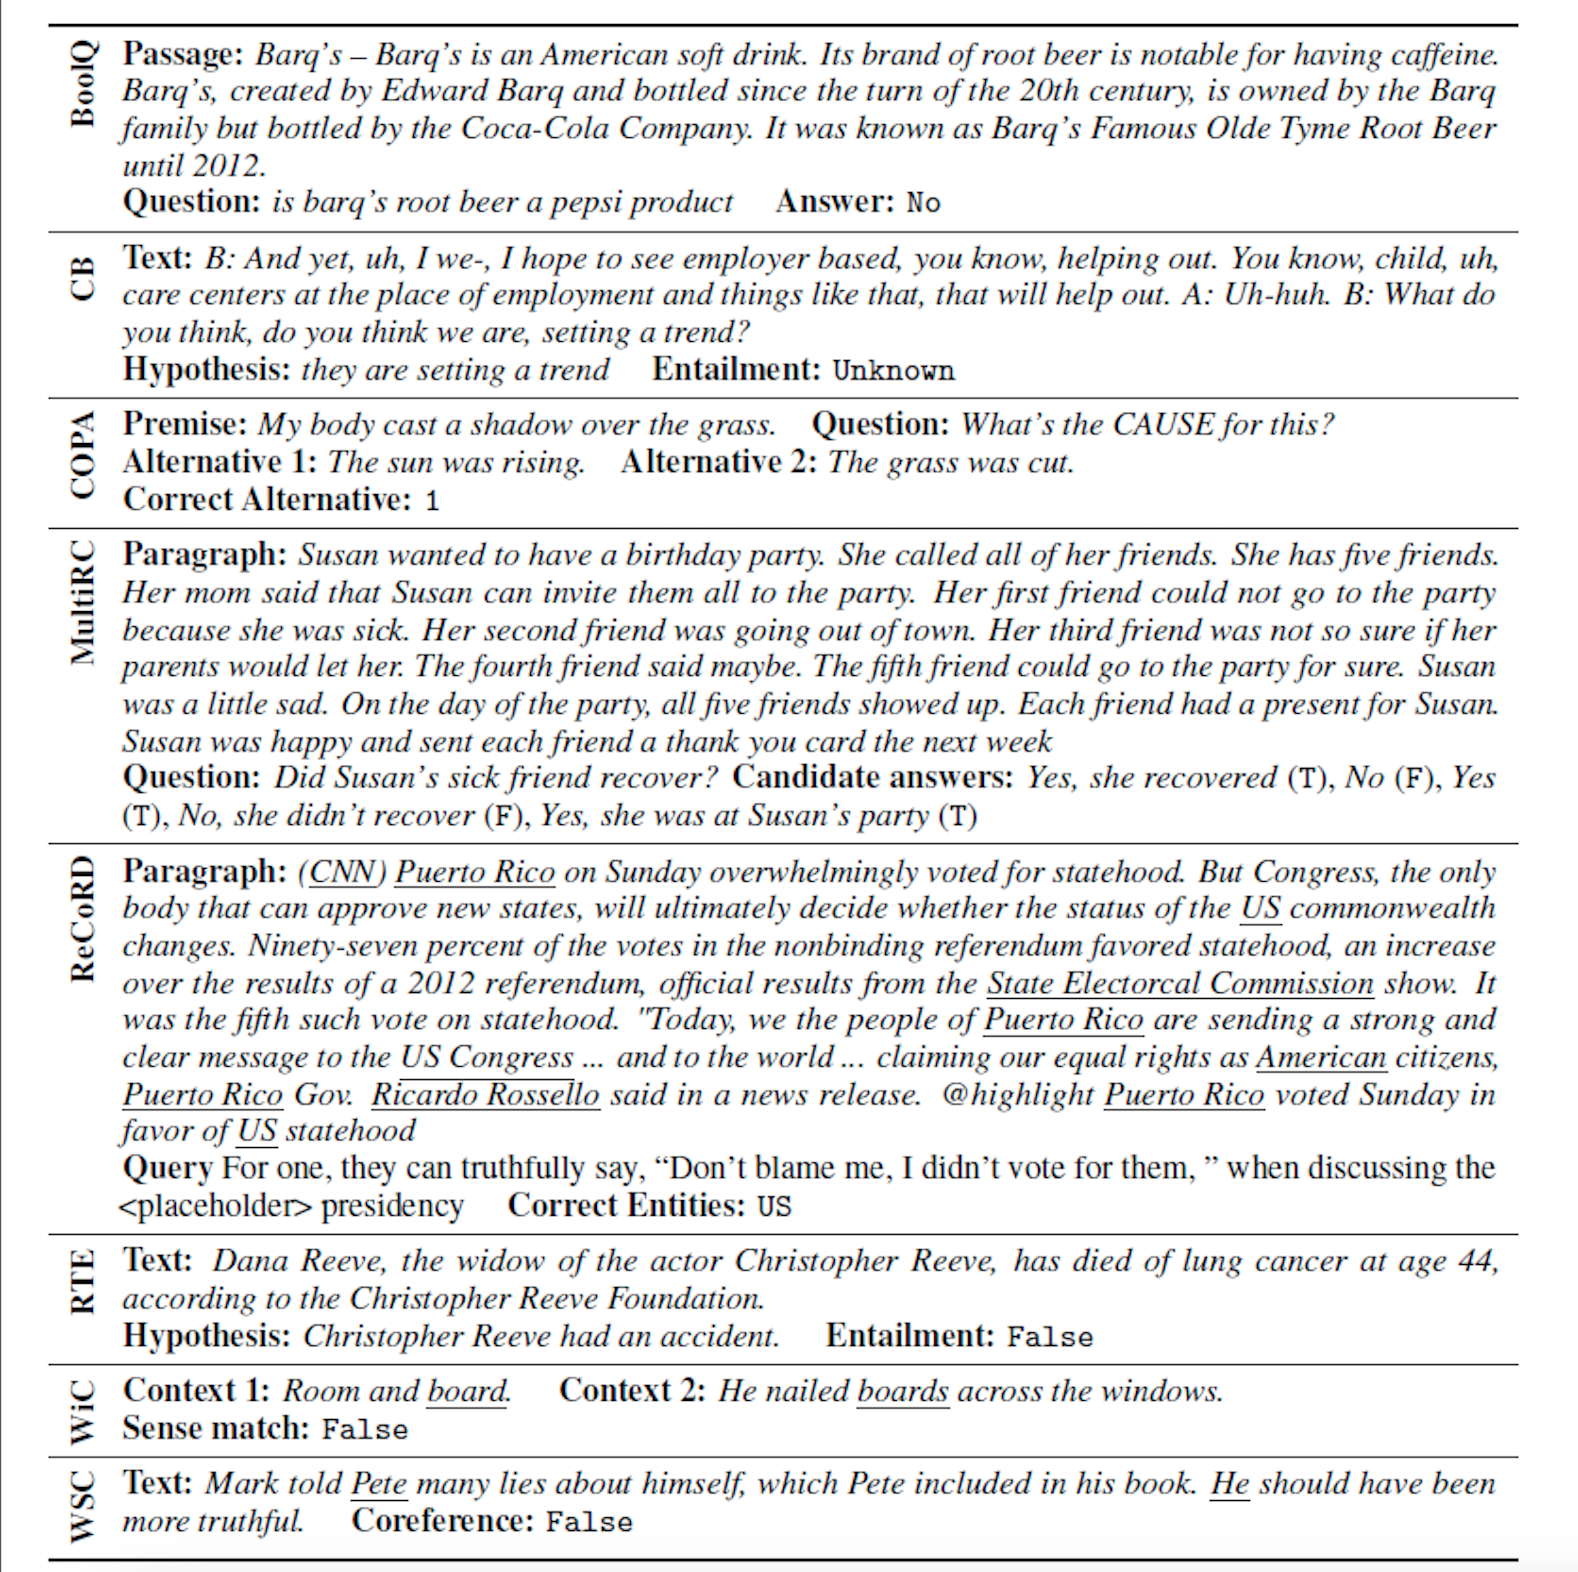
\includegraphics{figures/01-chapter1/SuperGLUE.png}
\caption{taken from \url{https://mccormickml.com}}
\end{figure}

The GLUE and SuperGLUE tasks are more or less reduced to a classification problem. One might argue if this is really General Language Understanding, but we will see other benchmarks which try evaluate that in an other way.

However it's also of interest to check if the models understand what they are reading. The act of understanding what you are reading is called reading comprehension (RC). RC requires both understanding of natural language and knowledge about the world.

\hypertarget{stanford-question-answering-dataset-squad-1.0-2.0}{%
\paragraph{Stanford Question Answering Dataset (SQuAD) (1.0 \& 2.0)}\label{stanford-question-answering-dataset-squad-1.0-2.0}}

\citet{rajpurkar2016squad} introduced the Stanford Question Answering Dataset (SQuAD), a large reading comprehension dataset on Wikipedia articles with human annotated question-answer pairs. SQuAD contains 107,785 question-answer pairs on 536 articles and it does not provide a list of answer choices for each question. The model must select the answer from all possible spans in the passage, thus needing to cope with a fairly large number of candidates. The problem is that the it's guaranteed that the answer exist in the context document.

To address this weakness \citet{rajpurkar2018know} presented SQuAD 2.0, the latest version of SQuAD. SQuAD 2.0 combines existing SQuAD data with over 50,000 unanswerable questions written adversarially by crowdworkers to look similar to answerable ones.

\citet{rajpurkar2018know} contribution to NLP is not that they provide a deeper glimpse into the workings of QA systems, they also facilitated the creation of more non-English datasets. Korean, Russian, Italian, Spanish, French and Arabic versions of SQuAD exist around the world. XQuAD, MLQA and TyDi are multilingual question-answering datasets. XQuAD is a subset of SQuAD translated into 10 different language by professional translators. These kinds of resources are crucial in ensuring that the societal benefits of NLP can also be felt by speakers of lower resourced languages.

\hypertarget{beyond-the-imitation-game-benchmark-big-bench}{%
\paragraph{Beyond the Imitation Game Benchmark (BIG-bench)}\label{beyond-the-imitation-game-benchmark-big-bench}}

The mentioned ones are rather old compared to Beyond the Imitation Game Benchmark (BIG-bench) \citep{srivastava2022beyond}. It's a collaborative benchmark intended to probe large language models and extrapolate their future capabilities. BIG-bench already contains more than 200 tasks. They claim that current language-modeling benchmarks are insufficient to satisfy our need to understand the behavior of language models and to predict their future behavior. They mainly provide three reasons for that. One of them is the short useful lifespans. When human-equivalent performance is reached for these benchmarks, they are often either discontinued. One might call this ``challenge-solve-and-replace'' evaluation dynamic.

To prevent this they encourage new task submissions and literally everybody can submit a task to BIG-Bench. So they call BIG-bench a living benchmark. The review of the tasks is based on ten criteria. It includes for example ``Justification''. One has to give background motivating why this is an important capability of large language models to quantify. With the inclusion of small tasks they want to improve the diversity of topics covered and enable domain experts to contribute tasks without the difficulties of distributed human labeling.

Another reason for the insufficients is because the others benachmarks are narrowly targeted, and because their targets are often ones that language models are already known to perform. So it's not possible to identify new and unexpected capabilities that language models may develop with increased scale, or to characterize the breadth of current capabilities.

Finally, many current benchmarks use data collected through human labeling that is not performed by experts or by the task authors. Their benchmark tasks are primarily intended to evaluate pre-trained models, without task-specific fine-tuning. By focusing on such tasks in the zero- and few-shot evaluation setting, it becomes possible to provide meaningful scores for even those tasks with a very small number of examples.

The ``everybody can submit'' strategy also leads to inclusion a variety of tasks covering non-English languages. Till now the large language models, like GPT-3 and PaLM, perform poorly on BIG-bench relative to expert humans, which is maybe a good sign for the future. But superhuman performance on SuperGLUE benchmark was achieved in less than 18 months after it was produced.

\hypertarget{wmt}{%
\paragraph{WMT}\label{wmt}}

There is a family of datasets which is the most popular datasets used to benchmark machine translation systems. \href{https://machinetranslate.org/wmt}{Workshop on Machine Translation (WMT)} is the main event for machine translation and machine translation research. This conference is held annually. WMT includes competitions on different aspects of machine translation. These competitions are known as shared tasks. Typically, the task organisers provide datasets and instructions. Then teams can submit their output of their models. The submissions are ranked with human evaluation.

Most of the models are evaluated on bi-lingual translation like English-to-German, but there are also tri-linguar tasks like using English to improve Russian-to-Chinese machine translation. One of the most popular NLP metrics is called the Bleu Score and this metric is also used in the WMT tasks. It is based on the idea that the closer the predicted sentence is to the human-generated target sentence, the better it is. Bleu Scores are between 0 and 1, but a score of 0.6 or 0.7 is considered the best you can achieve.

Problematic is that \citet{bowman2021will} claim that the evaluation for many natural language understanding (NLU) tasks are broken. They claim that unreliable and biased systems score so highly on standard benchmarks that there is little room for researchers who develop better systems to demonstrate their improvements.
They provide four criteria to handle this:

\begin{enumerate}
\def\labelenumi{\arabic{enumi}.}
\tightlist
\item
  Good performance on the benchmark should imply robust in-domain performance on the task
\item
  Benchmark examples should be accurately and unambiguously annotated
\item
  Benchmarks should offer adequate statistical power
\item
  Benchmarks should reveal plausibly harmful social biases in systems, and should not incentivize the creation of biased systems
\end{enumerate}

Building new benchmarks that improve upon these four axes is likely to be quite difficult.

\hypertarget{checklist}{%
\paragraph{CheckList}\label{checklist}}

Inspired by principles of behavioral testing in software engineering, \citet{ribeiro2020beyond} introduced CheckList, a model-agnostic and task-agnostic methodology for testing NLP models. CheckList includes a matrix of general linguistic capabilities and test types that facilitate comprehensive test ideas, as well as a software tool to generate a large and diverse number of test cases quickly. To break down potential capability failures into specific behaviors, CheckList introduces three different test types. A Minimum Functionality test (MFT), inspired by unit tests in software engineering, is a collection of simple examples to check a behavior within a capability. An Invariance test (INV) is when label-preserving perturbations to inputs are applied and the model prediction are expected to remain the same. A Directional Expectation test (DIR) is similar, except that the label is expected to change in a certain way.

Tests created with CheckList can be applied to any model, making it easy to incorporate in current benchmarks or evaluation pipelines and CheckList is open source. Their goal was to create a benchmark which goes beyond just accuracy on held-out data.

\hypertarget{computer-vision-benchmarks}{%
\subsubsection{Computer Vision Benchmarks}\label{computer-vision-benchmarks}}

CV models try to answer visual tasks. A visual task is a task which can be solved only by visual input. Often visual task can be solved as a binary classification problem, which is called image classification, but there are also numerous other applications for CV. This chapter will focus on image classification, semantic segmentation and object detection with their usual benchmarks datasets.

\hypertarget{imagenet-versions}{%
\paragraph{ImageNet Versions}\label{imagenet-versions}}

It's not only common to pre-train your model on ImageNet datasets it's also common to benchmark the models on them. There are many different variants of ImageNet. There is ImageNet-R, a version with non-natural images such as art, cartoons and sketches, or ImageNet-A, which is a a more challenging version because they use adversarial images \citep{goodfellow2014explaining}, or ImageNet-V2 \citep{recht2019imagenet}. The last was created to check whether there is an over-fitting on the classic pre-training ImageNet dataset. They followed the creation process of the original dataset and tested to what extent current classification models generalize to new data. \citet{recht2019imagenet} found accuracy drops for all models and suggested that these drops are not caused by adaptivity, but by the models' inability to generalize to slightly ``harder'' images than those found in the original test sets.

The goal of image classification is to classify the image by assigning a label. Typically, Image Classification refers to images in which only one object appears. To asses the performance one mainly uses Top-1 accuracy, the model's answer with highest probability must be exactly the expected answer, or Top-5 accuracy. Top-5 accuracy means that any of five highest probability answers must match the expected answer. \citet{beyer2020we} tried to answer the question ``Are we done with ImageNet?'' in their paper. Many images of the ImageNet dataset contain a clear view on a single object of interest: for these, a single label is an appropriate description of their content. However many other images contain multiple, similarly prominent objects, limiting the relevance of a single label \citep{beyer2020we}. In these cases, the ImageNet label is just one of many equally valid descriptions of the image and as a result an image classifier can be penalized for producing a correct description that happens to not coincide with that chosen by the ImageNet label.

In short a single label per image is not sufficient in many cases. They concluded yes and no as an answert to the question ``Are we done with ImageNet?''. The shortcomings of ImageNet labels and their accuracy were identified and they provided a new ImageNet validation set ReaL \citep{beyer2020we} (``Reassessed Labels'') and also a new metric, called ReaL accuracy \citep{beyer2020we}. The ReaL accuracy measures the precision of the model's top-1 prediction, which is deemed correct if it is included in the set of labels. these findings suggested that although the original set of labels may be nearing the end of their useful life, ImageNet and its ReaL labels can readily benchmark progress in visual recognition for the foreseeable future.

An addition of a localization tasks to the classification tasks results into object detection. It is used to analyze more realistic cases, like mentioned above, in which multiple objects may or may not exist in an image. The location of an object is typically represented by a bounding box.

\hypertarget{ms-coco-object365}{%
\paragraph{MS-COCO \& Object365}\label{ms-coco-object365}}

In the recent years, the Microsoft COCO dataset or the Object365 data have become the standards to evaluate object detection algorithms, but it's also possible to use a ImageNet dataset. The primary challenge metric is called mean Average Precision (mAP) at Intersection over Union (IoU) \(=\).50:.05:.95. The IoU is the intersection of the predicted and ground truth boxes divided by the union of the predicted and ground truth boxes. IoU, also called Jaccard Index, values range from 0 to 1. Where 0 means no overlap and 1 means perfect overlap. But how is precision captured in the context of object detection? Precision is known as the ratio of \(True~Positive/(True~Positive+False~Positive)\). With the help of the IoU threshold, it's possible to decide whether the prediction is True Positive(TP), False Positive(FP), or False Negative(FN). The example below shows predictions with IoU threshold ɑ set at 0.5.

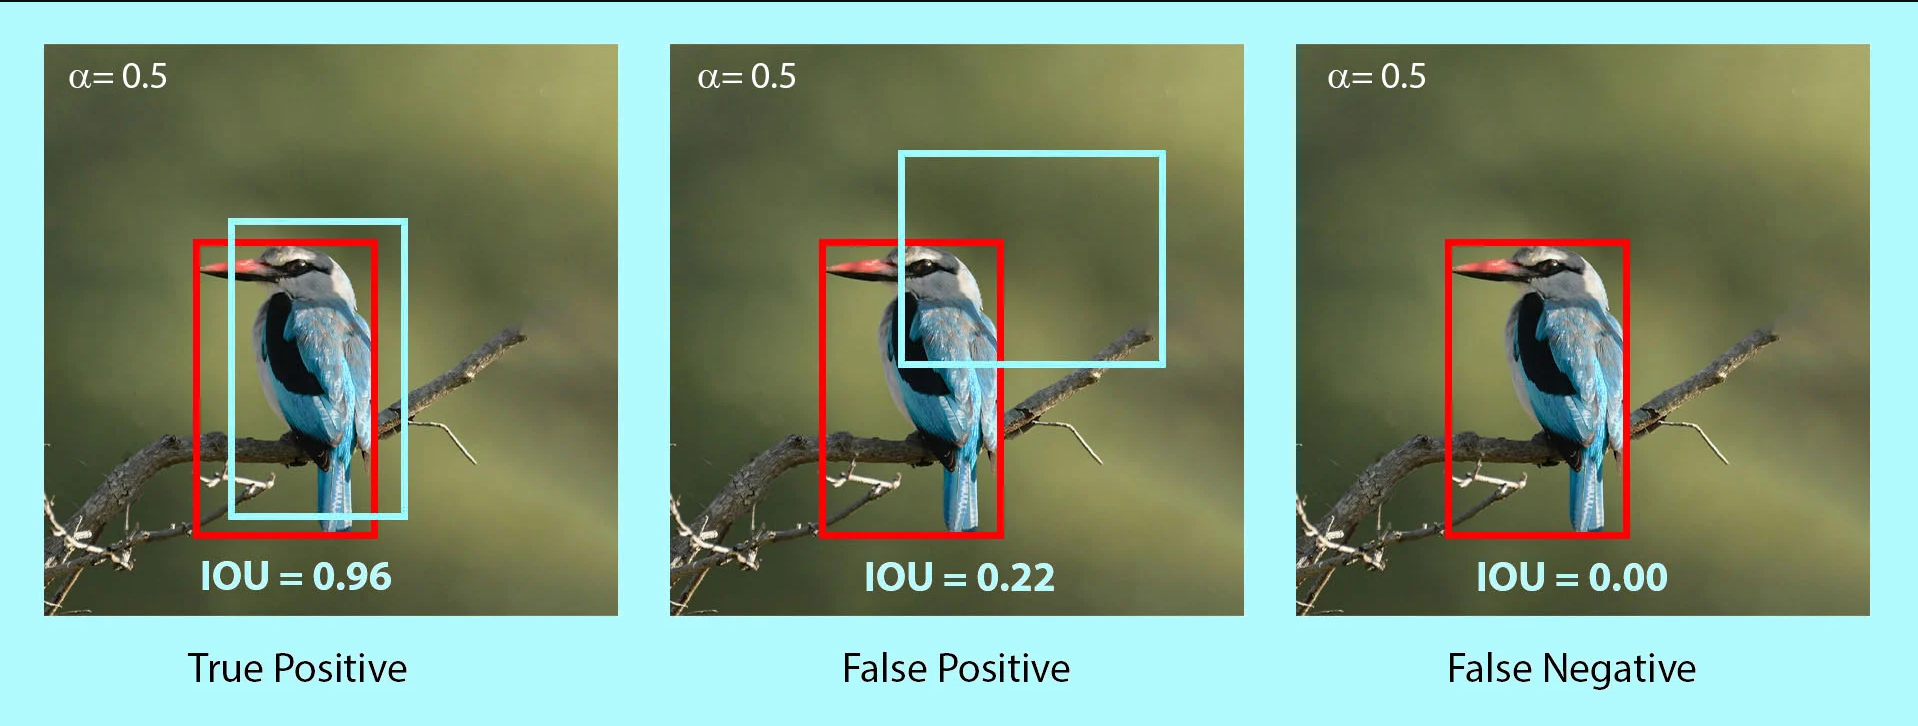
\includegraphics{figures/01-chapter1/4-birds-prediction-types-1.png}
The .50:.05:.95 means that one uses 10 IoU thresholds of \(\{0.50, 0.55, 0.60, \dots ,0.95\}\). COCO uses this as primary metric, because it rewards detectors with better localization \citep{coco_eval}.

Object detection and image segmentation are both tasks which are concerned with localizing objects of interest in an image, but in contrast to object detection image segmentation focuses on pixel-level grouping of different semantics.

Image segmentation can be splitted into various tasks including instance segmentation, panoptic segmentation, and semantic segmentation. Instance segmentation is a task that requires the identification and segmentation of individual instance in an image. Semantic segmentation is a task that requires segmenting all the pixels in the image based on their class label. Panoptic segmentation is a combination of semantic and instance segmentation. The task is to classify all the pixels belonging to a class label, but also identify what instance of class they belong to. Panoptic and instance segmentation is often done on COCO.

\hypertarget{ade20k}{%
\paragraph{ADE20k}\label{ade20k}}

Semantic segmentation can be done one ADE20K\citep{zhou2017scene}. ADE are the first three letters of the name Adela Barriuso, who single handedly annotated the entire dataset and 20K is a reference to being roughly 20,000 images in the dataset. This dataset shows a high annotation complexity, because any image in ADE20K contains at least five objects, and the maximum number of object instances per image reaches 273. To asses the performance of a model on the ADE20K dataset one uses the mean IoU. It indicates the IoU between the predicted and ground-truth pixels, averaged over all the classes.

In contrast to the object detection task, the definition of TP, FP, and FN is slightly different as it is not based on a predefined threshold. TP is now the area of intersection between Ground Truth and segmentation mask. FP is the predicted area outside the Ground Truth. FN is the number of pixels in the Ground Truth area that the model failed to predict. The calculation of IoU is the same as in object detection tasks. It's the intersection of the predicted and ground truth boxes aka. TP divided by the union of the predicted and ground truth boxes, which is essentially \(TP + FN + FP\).
A example is shown down below.

\begin{figure}
\centering
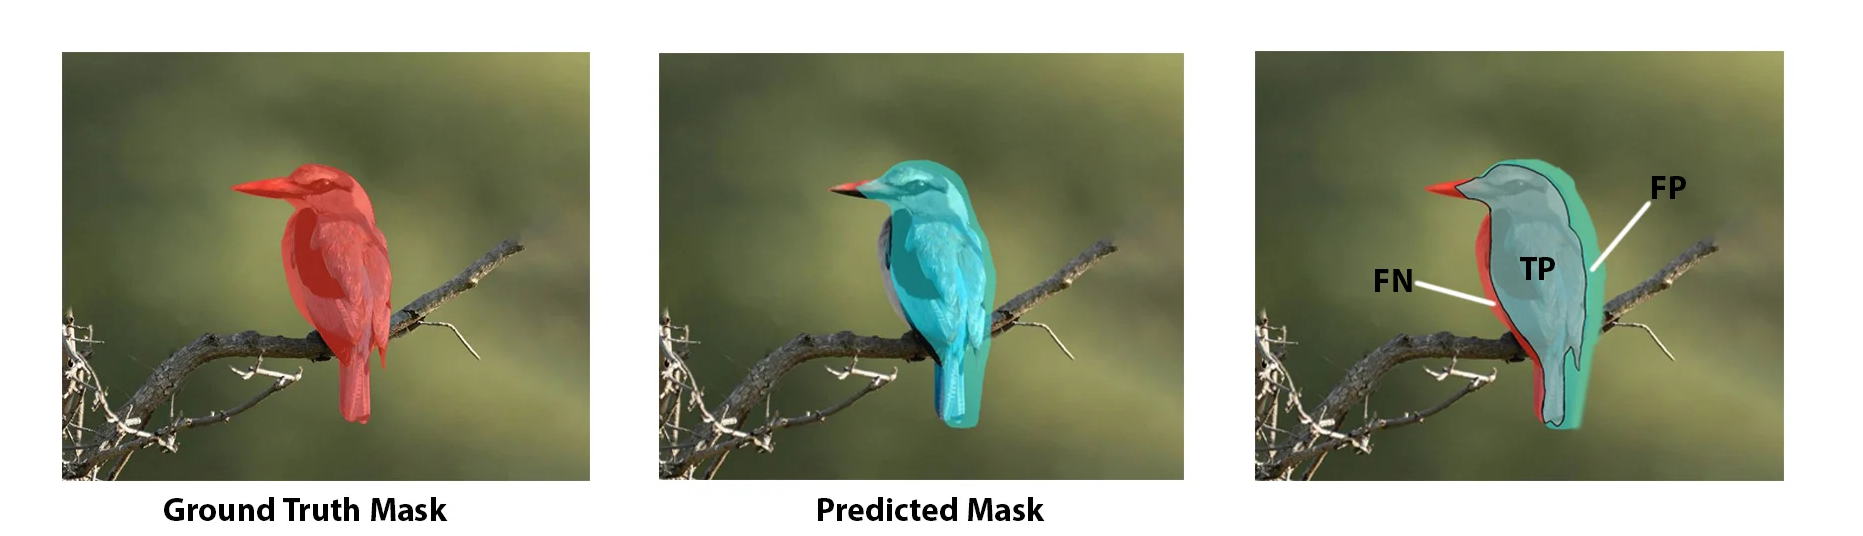
\includegraphics{figures/01-chapter1/5-segmentation-iou.png}
\caption{taken from \url{https://learnopencv.com}}
\end{figure}

\hypertarget{multi-modal-benchmarks}{%
\subsubsection{Multi-Modal Benchmarks}\label{multi-modal-benchmarks}}

Visual understanding goes well beyond object recognition or semantic segmentation. With one glance at an image, a human can effortlessly imagine the world beyond the pixels. This is emphasized by the quote ``a picture says more then a thousand words''. High-order of cognition and commonsense reasoning about the world is required to infer people's actions, goals, and mental states. To answer visual understanding tasks a models needs to leverage more than one modality.

\hypertarget{visual-commonsense-reasoning-vcr}{%
\paragraph{Visual Commonsense Reasoning (VCR)}\label{visual-commonsense-reasoning-vcr}}

Visual understanding tasks require seamless integration between recognition and cognition and this task can be formalize as Visual Commonsense Reasoning (VCR). \citet{zellers2019recognition} introduce a new dataset called VCR. It consists of 290k multiple choice QA problems derived from 110k movie scenes. The key recipe for generating non-trivial and high-quality problems at scale is Adversarial Matching. Incorrect choices are obtained via maximum-weight bipartite matching between queries and responses. This matching transforms rich annotations into multiple choice questions with minimal bias. VCR casted as a four-way multiple choice task.

The underlying scenes come from the Large Scale Movie Description Challenge and YouTube movie clips and they searched for interesting an diverse situations to ensure this they trained and applied an ``interestingnes filter''. The most interesting images were passed to Workers of Amazon Mechanical Turk. Additional context in form of video caption was given to the worker. After reading this they had to propose one to three questions about the image. For each question, they had to provide a reasonable answer and a rationale. This results is an underlying dataset with high agreement and diversity of reasoning. Almost every answer and rationale is unique. To make these cognition-level questions simple to ask, and to avoid the clunkiness of referring expressions, VCR's language integrates object tags ({[}person2{]}) and explicitly excludes referring expressions (`the woman on the right.'). These object tags are detected from Mask-RCNN. The following types of questions are in the benchmarks: 38\% Explanation (`Why is {[}person11{]} wearing sunglasses inside?'), 24\% Activity ('What are {[}person1{]} and person{[}2{]} doing?``), 13\% Temporal (''What will {[}person6{]} do after unpacking the groceries?"), 8\% Mental, 7\% Role, 5\% Scene, 5\% Hypothetical.

So in this setup, a model is provided a question, and has to pick the best answer out of four choices. Only one of the four is correct. If the model answered correctly a new question, along with the correct answer, is provided. Now the model has to justify it by picking the best rationale out of four choices. The first part is called Question Answering (\(Q\rightarrow A\)) and the second part Answer Justification (\(QA\rightarrow R\)). They combine both parts into a \(Q\rightarrow AR\) metric, in which a model only gets a question right if it answers correctly and picks the right rationale. If it gets either the answer or the rationale wrong, the entire prediction will be wrong. Models are evaluated in terms of accuracy.

The results at the release were that humans find VCR easy (over 90\% accuracy), and state-of-the-art vision models struggle (∼45\%). At the moment of writing, the best model achieves 85.5 in (\(Q\rightarrow A\)), 87.5 in (\(QA\rightarrow R\)) and 74.9 in \(Q\rightarrow AR\). So the models are closing the gap but VCR is still far from solved. An ``simpler'' approach to evaluate vision-language models is to ask questions without reasoning about an image.

\hypertarget{visual-question-answering-1.0-2.0-vqa}{%
\paragraph{Visual Question Answering 1.0 \& 2.0 (VQA)}\label{visual-question-answering-1.0-2.0-vqa}}

For this reason \citet{antol2015vqa} created an open-ended answering task and a multiple-choice task. Their dataset contains roughly 250k images, 760k questions, and 10M answers. 204k images are taken from the MS COCO dataset but also newly created created datasets are used. Three questions were collected for each image or scene. Each question was answered by ten subjects along with their confidence. The dataset contains over 760K questions with around 10M answers. ``what''-, ``how''-, ``is''- questions are mainly used in the benchmark. But they had major flaws in their creation. An model which blindly answering ``yes'' without reading the rest of the question or looking at the associated image results in a VQA accuracy of 87\% or the most common sport answer ``tennis'' was the correct answer for 41\% of the questions starting with ``What sport is'', and ``2'' is the correct answer for 39\% of the questions starting with ``How many'' \citep{antol2015vqa}.

\citet{zhang2016yin} pointed out a particular `visual priming bias' in the VQA dataset. \citet{zhang2016yin} showed that language provides a strong prior that can result in good superficial performance, without the underlying models truly understanding the visual content. \citet{zhang2016yin} collected a balanced dataset containing pairs of complementary scenes to reduce or eliminate the strong prior of the language. \citet{goyal2017making} did the same and made a second iteration of the Visual Question Answering Dataset and Challenge (VQA v2.0). \citet{goyal2017making} balanced the popular VQA dataset \citep{antol2015vqa} by collecting complementary images such that every question in balanced dataset is associated with not just a single image, but rather a pair of similar images that result in two different answers to the question. The dataset is by construction more balanced than the original VQA dataset and has approximately twice the number of image-question pairs.

\hypertarget{gqa}{%
\subsubsection{GQA}\label{gqa}}

\citet{hudson2019gqa} introduced the GQA dataset for real-world visual reasoning and compositional question answering. It consists of 113K images and 22M questions of assorted types and varying compositionality degrees, measuring performance on an array of reasoning skills such as object and attribute recognition, transitive relation tracking, spatial reasoning, logical inference and comparisons. They also proposed Consistency, Validity and Plausibility as new measures to get more insight into models' behavior and performance. Consistency measures responses consistency across different questions. To achieve a high consistency a model may require deeper understanding of the question semantics in context of the image. The validity metric checks whether a given answer is in the question scope, e.g.~responding some color to a color question. The plausibility score goes a step further, measuring whether the answer is reasonable, or makes sense, given the question (e.g.~elephant usually do not eat pizza).

They even made a comparison between GQA and VQA 2.0. They came to the conclusion that the questions of GQA are objective, unambiguous, more compositional and can be answered from the images only, potentially making this benchmark more controlled and convenient for making research progress on. Conversely, VQA questions tend to be a bit more ambiguous and subjective, at times with no clear and conclusive answer. Finally, we can see that GQA provides more questions for each image and thus covers it more thoroughly than VQA.

\hypertarget{generative-benchmarks}{%
\paragraph{Generative Benchmarks}\label{generative-benchmarks}}

Almost everybody is talking right now about generative models like DALL-E2, Imagen, Parti. It seems like every month a new one is presented. But how can we compare these models? Automatic image quality and automatic image-text alignment are two reasonable evaluation metrics. Fréchet Inception Distance (FID) can be used as primary automated metric for measuring image quality. The Frechet Inception Distance compares the distribution of generated images with the distribution of real images that were used to train the generator. A small value is wanted, as it's a distance measure. Text-image fit can be captured through automated captioning evaluation. For this an image output by the model is captioned with a model, which is able to do image captioning. The similarity of the input prompt and the generated caption is then assessed via BLEU, CIDEr, METEOR and SPICE and also human evaluation is done. Here different generative models are used with the same prompts and the human is asked to choose which output is a higher quality image and which is a better match to the input prompt. One always has to keep in mind, that the images of the generative models are always ``cherry picked''. They do not typically represent, for example, a single shot interaction in which the model directly produces such an image. To make this clear, \citet{parti} showed their way of growing the cherry tree.

\begin{figure}
\centering
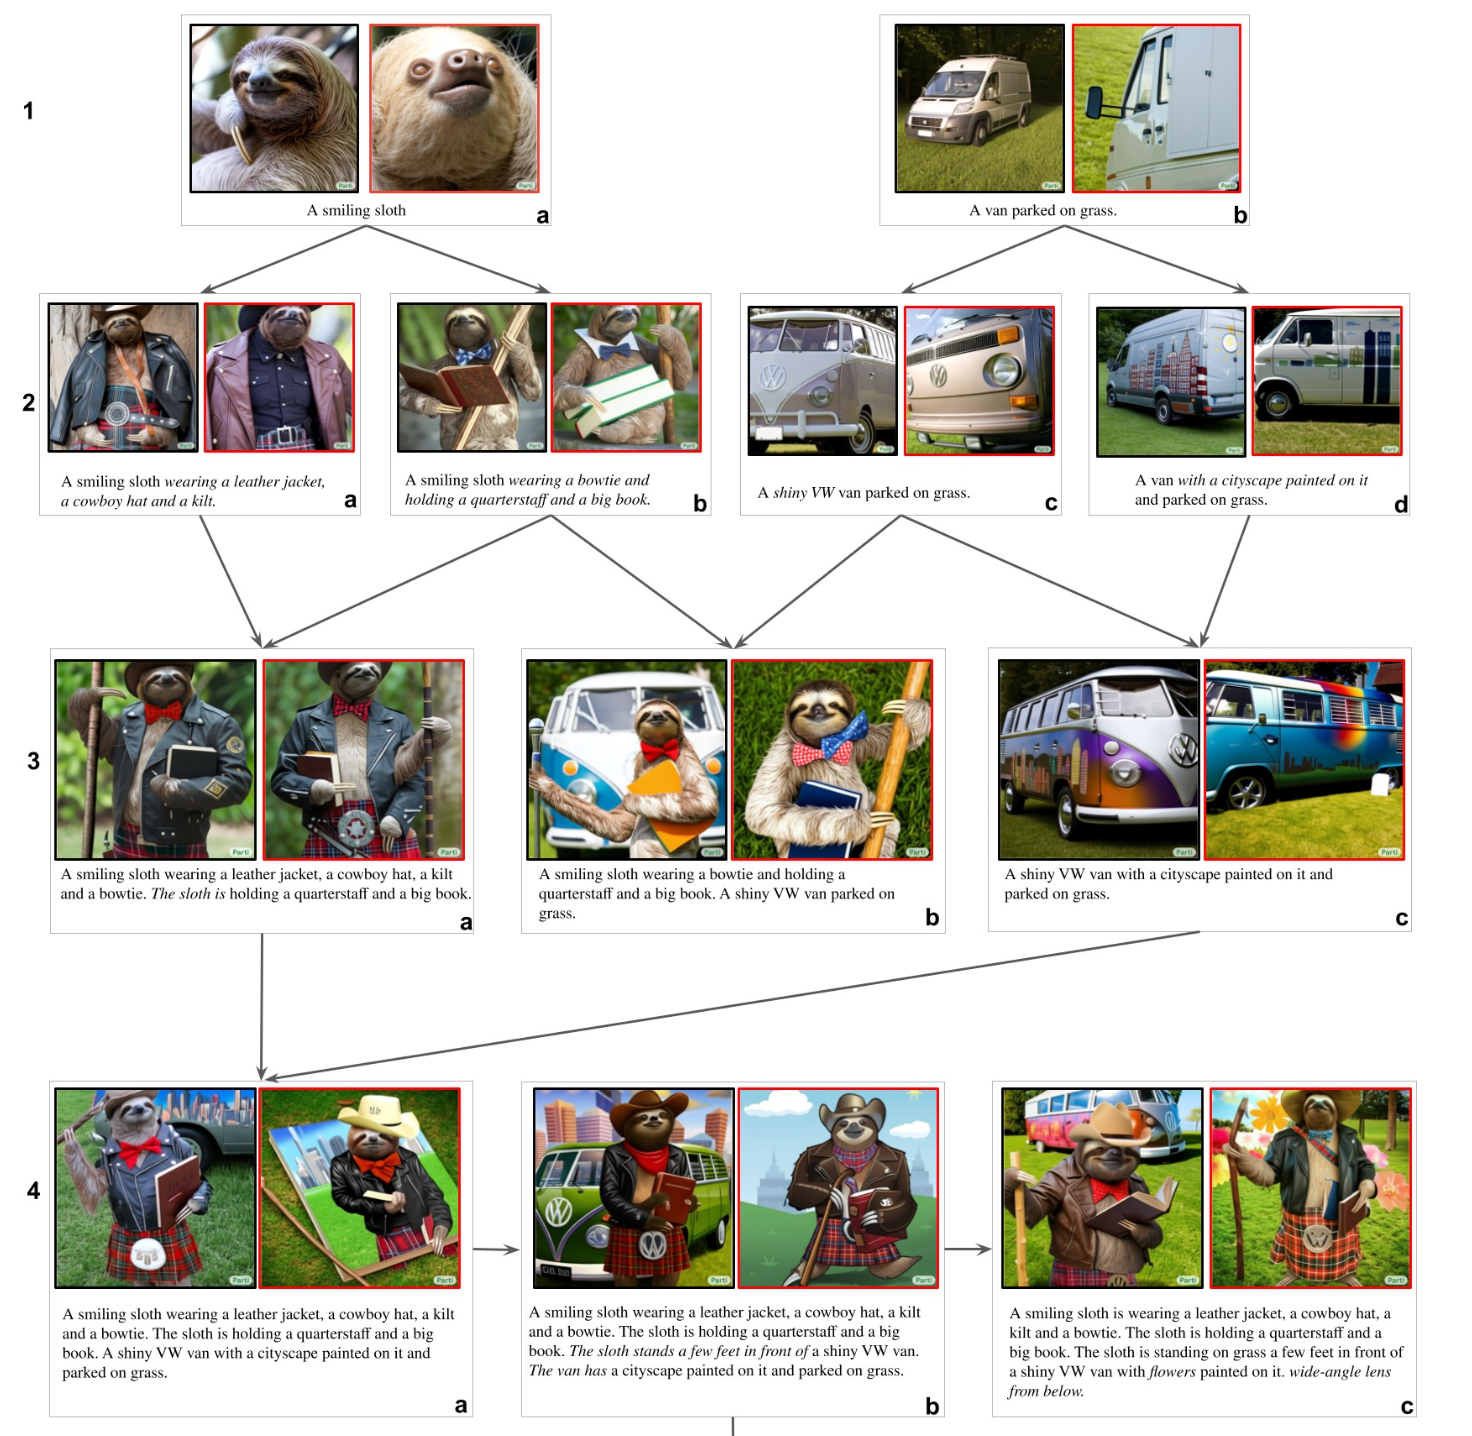
\includegraphics{figures/01-chapter1/Parti_Growing.png}
\caption{taken from Parti Paper}
\end{figure}

\hypertarget{partiprompts-drawbench-localized-narratives}{%
\paragraph{PartiPrompts, DrawBench, Localized Narratives}\label{partiprompts-drawbench-localized-narratives}}

In a sense, this is a form of model whispering as one stretches such models to their limits. Besides to that they also present PartiPrompts (P2) which is a set of over 1600 (English) prompts curated to measure model capabilities across a variety of categories and controlled dimensions of difficulty. P2 prompts can be simple, but can also be complex, such as 67-word description they created for Vincent van Gogh's The Starry Night. DrawBench is a similar dataset. Also the Localized Narratives dataset from the dataset section consists of long prompts and though it can also be used as a benchmark for generative models.

Current benchmarks give a good perspective on model performance on a wide range of V\&L tasks, but the field is only starting to assess why models perform so well and whether models learn specific capabilities that span multiple V\&L tasks.

\hypertarget{foil-it}{%
\paragraph{FOIL it!}\label{foil-it}}

\citet{shekhar2017foil} proposed an automatic method for creating a large dataset of real images with minimal language bias and some diagnostic abilities. They extended the MS-COCO dataset and created FOIL-COCO. FOIL stands for ``Find One mismatch between Image and Language caption'' and consists of images associated with incorrect captions. The captions are produced by introducing one single error (or `foil') per caption in existing, human-annotated data. So each datapoint FOIL-COCO can be described as triplet consisting of an image, original and foil caption. Their data generation process consists of four main steps:

\begin{enumerate}
\def\labelenumi{\arabic{enumi}.}
\tightlist
\item
  Generation of replacement word pairs
\item
  Splitting of replacement pairs into training and testing
\item
  Generation of foil captions
\item
  Mining the hardest foil caption for each image
\end{enumerate}

The models are evaluated on three different tasks. The first one is Correct vs.~foil classification. Given an image and a caption, the model is asked to mark whether the caption is correct or wrong. The aim is to understand whether LaVi models can spot mismatches between their coarse representations of language and visual input. The second task is Foil word detection. Given an image and a foil caption, the model has to detect the foil word. The aim is to evaluate the understanding of the system at the word level. The last task Foil word correction. Given an image, a foil caption and the foil word, the model has to detect the foil and provide its correction. The aim is to check whether the system's visual representation is fine-grained enough to be able to extract the information necessary to correct the error. Their hypothesis is that systems which, like humans, deeply integrate the language and vision modalities, should spot foil captions quite easily.

\hypertarget{valse}{%
\paragraph{VALSE}\label{valse}}

Vision And Language Structured Evaluation (VALSE) \citep{parcalabescu-etal-2022-valse} builds on the same idea. This benchmark aims to gauge the sensitivity of pre-trained V\&L models to foiled instances. They coverd a wide spectrum of basic linguistic phenomena affecting the linguistic and visual modalities: existence, plurality, counting, spatial relations, actions, and entity coreference. To generate the foils they first use strong language models to propose foil and second they use natural language inference to filter out captions that still can describe the image. To do this in an automatic fashion they use the image as an premise and the caption its entailed hypothesis. Additionally they use the captian as an premise and the foil as the hypothesis. If an NLI model predicts the foil to be neutral or a contradiction with respect to the caption, they see this as an indicator for a good foil. At last the used human annotators to validate all generated testing data. Mainly the MS-COCO dataset is used. VALSE is as a task-independent, zero-shot benchmark to assess the extent to which models learn to ground specific linguistic phenomena as a consequence of their pretraining.

\hypertarget{other-benchmarks}{%
\subsubsection{Other Benchmarks}\label{other-benchmarks}}

As we don't live in a world with unlimited resources, it's also important to keep track of how much energy is consumed to train the models and how big the carbon footprint is. \citet{strubell2019energy} investigated some NLP models and benchmarked model training and development costs in terms of dollars and estimated \(CO_2\) emissions. They came to the result that training a single BERT base model without hyperparameter tuning on GPUs requires the same energy as a trans-American flight. On average a human is responsible for 5t \(CO_2\) per year and \citet{strubell2019energy} estimated that the training procedure of a big Transformer with neural architecture search emitted 284t of \(CO_2\). Works \citep[\citet{henderson2020towards}]{lottick2019energy} have released online tools to benchmark their energy usage and initiatives such as the \href{https://sites.google.com/view/sustainlp2020/organization}{SustainNLP workshop} have since taken up the goal of prioritizing computationally efficient hardware and algorithms. These findings are just some points one should keep in mind.

In the following chapters we will see how the multimodal architectures use these datasets and also how they perform on the given benchmarks.

\hypertarget{c02-00-multimodal}{%
\chapter{Multimodal architectures}\label{c02-00-multimodal}}

\emph{Authors: Luyang Chu, Karol Urbanczyk, Giacomo Loss, Max Schneider, Steffen Jauch-Walser}

\emph{Supervisor: Christian Heumann}

Multimodal learning refers to the process of learning representations from different types of input modalities, such as image data, text or speech.
Due to methodological breakthroughs in the fields of Natural Language Processing (NLP) as well as Computer Vision (CV), in recent years multimodal models have gained increasing attention as they are able to strengthen predictions and better emulate the way humans learn.
This chapter focuses on discussing images and text as input data.
The remainder of the chapter is structured as follows:

The first part ``Image2Text'' discusses how transformer-based architectures improve meaningful captioning for complex images using a new large scale, richly annotated dataset COCO \citep{mccoco, cornia2020m2}.
Whether it is seeing a photograph and describing it or parsing a complex scene and describing its context, it is not a difficult task for humans.
But it is much more complex and challenging for computers.
We start with focusing on images as input modalities.
In 2014 Microsoft COCO was developed with a primary goal of advancing the state-of-the-art (SOTA) in object recognition by diving deeper into a broader question of scene understanding \citep{mccoco}.
COCO stands for Common Objects in Context.
It addresses three core problems in scene understanding: object detection (non-iconic views), segmentation, and captioning.
For tasks like machine translation and language understanding in NLP, transformer-based architecture is widely used.
However, the potential of these applications in the multi-modal context has not been fully covered.
With the help of the COCO dataset, a transformer-based architecture: Meshed-Memory Transformer for Image Captioning (\(M^2\)) will be introduced to improve both image encoding and the language generation steps \citep{cornia2020m2}.
The performance of the (\(M^2\)) Transformer and different fully-attentive models will be evaluated and compared on the COCO dataset.

Next, in ``Text2Image'', the idea of incorporating textual input in order to generate visual representations is described.
Current advancements in this field have been made possible largely due to recent breakthroughs in NLP, which first allowed for learning contextual representations of text.
Transformer-like architectures are being used to encode the input into embedding vectors, which are later helpful in guiding the process of image generation.
The chapter looks into details and discusses two SOTA model architectures by OpenAI, which both condition on text representations.
Surprisingly, none of them uses a GAN approach - a method which probably has been seen as the go-to idea for image generation over the last years.
The first model is DALL-E \citep{ramesh2021dalle}, which essentially combines Variational Encoder (VAE) with Autoregressive Transformer.
In the first step, VAE is being trained to learn downsized image representations.
Such embeddings are concatenated with text embeddings into one text-image pair input.
However, both of them use different dimensionality and vocabulary size.
In the second step, the transformer is trained on a next token prediction task given these data pairs.
Finally, at inference time, the model is able to generate images in the following way:

\begin{enumerate}
\def\labelenumi{\arabic{enumi}.}
\tightlist
\item
  Encode text input into text embedding
\item
  Use trained transformer from step 2 to generate image embedding
\item
  Use VAE from step 1 to generate image from image embedding
\end{enumerate}

The next approach to text-to-image generation is a GLIDE model \citep{nichol2021glide}.
GLIDE stands for Guided Language to Image Diffusion for Generation and Editing.
Its idea is to use Diffusion Models.
In its core, Diffusion Model is a simple idea -- random noise is being added to the image in an iterative fashion, and then model learns how to reconstruct this image.
In the case of GLIDE this learning process is conditioned on the text prompt, which is first passed through a transformer.
Both models differ in their results.
While DALL-E's resulting images might have been overwhelming back in the beginning of 2021, GLIDE is thought to significantly improve on photorealism and resolution the generated images.
Since the field has already seen further improvements following GLIDE, these new developments are also going to be mentioned in the chapter.

The third part, ``Images supporting Language Models'', deals with the integration of visual elements in pure textual language models.
Distributional semantic models such as Word2Vec and BERT assume that the meaning of a given word or sentence can be understood by looking at how (in which context) and when the word or the sentence appear in the text corpus, namely from its ``distribution'' within the text.
But this assumption has been historically questioned, because words and sentences must be grounded in other perceptual dimensions in order to understand their meaning \citep[see for example the ``symbol grounding problem'';][]{harnad1990symbol}.
For these reasons, a broad range of models has been developed with the aim to improve pure language models, leveraging on the addition of other perceptual information, such as visual ones.
This subchapter focuses in particular on the integration of visual elements (images) to support pure language models for various tasks at the word-level and sentence-level.
The starting point is always a language model, on which visual representations (extracted often with the help of large pools of images like MS COCO, see chapter ``Img2Text'' for further references) are to be ``integrated''.
But how?
There has been proposed a wide range of solutions:
On one side of the spectrum, textual elements and visual ones are learned separately and then ``combined'' together whereas on the other side, the learning of textual and visual features takes place simultaneously/jointly.

\begin{figure}

{\centering 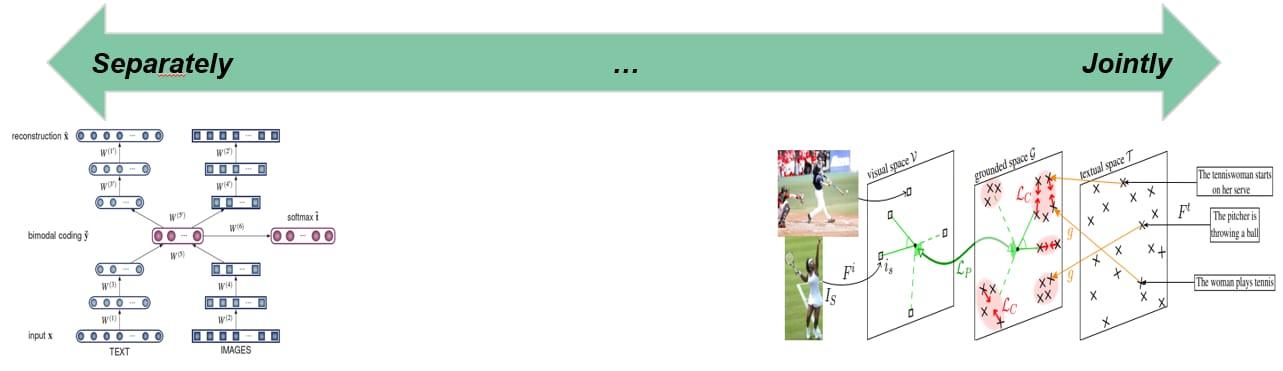
\includegraphics[width=1\linewidth]{figures/02-chapter2/Img_Ch_Intro} 

}

\caption{Left, Silberer et al., 2014: stacked autoencoders to learn higher-level embeddings from textual and visual modalities, encoded as vectors of attributes. Right, Bordes et al., 2020: textual and visual information fused in an Intermediate space denoted as “grounded space”; the “grounding objective function” is not applied directly on sentence embeddings but trained on this intermediate space, on which sentence embeddings are projected.}\label{fig:unnamed-chunk-1}
\end{figure}

For example, \citet{silberer2012grounded} implement a model where a one-to-one correspondence between textual and visual space is assumed.
Text and visual representations are passed to two separate unimodal encoders and both outputs are then fed to a bimodal autoencoder.
On the other side, \citet{bordes2020incorporating} propose a ``text objective function'' whose parameters are shared with an additional ``grounded objective function''.
The training of the latter takes place in what the authors called a ``grounded space'', which allows to avoid the one-to-one correspondence between textual and visual space.
These are just introductory examples and between these two approaches there are many shades of gray (maybe more than fifty\ldots).
These models exhibit in many instances better performance than pure language models, but they still struggle on some aspects, for example when they deal with abstract words and sentences.

Afterwards, in ``Text supporting Image Models'', approaches where natural language is used as supervision for CV models are described.
Intuitively these models should be more powerful compared to models supervised solely by manually labeled data, simply because there is much more training data available.

An important example for this is the CLIP model \citep{radford2021learning} with its new dataset WIT (WebImageText) comprising 400 million text-image pairs scraped from the internet.
Similar to ``Text2Image'' the recent successes in NLP have inspired new approaches in this field.
Most importantly pre-train methods, which directly learn from raw text \citep[e. g. GPT-n, Generative Pre-trained Transformer;][]{brown2020language}.
So, CLIP stands for Contrastive Language-Image Pre-training.
A transformer-like architecture is used for jointly pre-training a text encoder and an image encoder.
For this the contrastive goal to correctly predict which natural language text pertains to which image inside a certain batch, is employed.
Training this way turned out to be more efficient than to generate captions for images.
This leads to a flexible model, which at test time uses the learned text encoder as a ``zero-shot'' classifier on embeddings of the target dataset's classes.
The model, for example, can perform optical character recognition, geo-location and action-recognition.
Performance-wise CLIP can be competitive with task-specific supervised models, while never seeing an instance of the specific dataset before.
This suggests an important step towards closing the ``robustness gap'', where machine learning models fail to meet the expectations set by their previous performance -- especially on ImageNet test-sets -- on new datasets.

Finally, ``Text plus Images'' discusses how text and image inputs can be incorporated into a single unifying framework in order to get closer to a general self-supervised learning model.
There are two key advantages that make such a model particularly interesting.
Similar to models mentioned in previous parts, devoid of human labelling, self-supervised models don't suffer from the same capacity constraints as regular supervised learning models.
On top of that, while there have been notable advances in dealing with different modalities using single modality models, it is often unclear to which extend a model structure generalizes across different modalities.
Rather than potentially learning modality-specific biases, a general multipurpose framework can help increase robustness while also simplifying the learner portfolio.
In order to investigate different challenges and trends in vision-and-language modelling,
this section takes a closer look at three different models, namely data2vec (\citet{baevski2022data2vec}), VilBert (\citet{lu2019vilbert}) and Flamingo (\citet{alayrac2022flamingo})
Data2vec is a new multimodal self-supervised learning model which uses a single framework for either speech, natural language processing or computer vision.
This is in contrast to earlier models which used different algorithms for different modalities.
The core idea of data2vec, developed by MetaAI, is to predict latent representations of the full input data based on a masked view of the input in a self-distillation setup using a standard transformer architecture. (\citet{baevski2022data2vec})
As a result, the main improvement is in the framework itself, not the underlying models themselves.
For example, the transformer architecture being used follows \citet{vaswani2017attention}.
Through their parallelizability, transformers have several advantages over CNNs particularly when
large amounts of data are being used, making them the standard approach in vision-language modelling. (\citet{dosovitskiy2020image})
VilBert is an earlier model that in contrast to data2vec can handle cross-modality tasks.
Finally, Flamingo is a modern few shot learning model which features 80B parameters -
significantly more than the other two models. Through a large language model incorporated in its architecture, it has great text generating capabilities to tackle open-ended tasks. It also poses the question how to efficiently train increasingly large models and shows the effectiveness of using perceiver architectures (\citet{jaegle2021perceiver}) to encode inputs from different modalities as well as how to leverage communication between pretrained and frozen models.

\hypertarget{c02-01-img2text}{%
\section{Image2Text}\label{c02-01-img2text}}

*Author: Luyang Chu

*Supervisor: Christian Heumann

Image captioning means autonomously producing descriptive sentences for images. It has stimulated interest in both natural language processing and computer vision research in recent years. Image captioning is a key task that requires a semantic comprehension of images as well as the capacity to generate accurate and precise description sentences.

\hypertarget{microsoft-coco-common-objects-in-context}{%
\subsection{Microsoft COCO: Common Objects in Context}\label{microsoft-coco-common-objects-in-context}}

Understanding of visual scenes plays an important role in computer vision research (CV).Many tasks are included in it, such as image classification, object detection, object localization and semantic scene labeling.
Through the computer vision research history, Image Datasets have played a critical role. They are not only essential for training and evaluating new algorithms, but also lead the research to new challenging directions.\citep{mccoco} In the early year, researchers developed Datasets \citep{deng2009imagenet},\citep{sun},\citep{pascalvoc} which enabled the direct comparison of hundreds of image recognition algorithms, that was the early evolution in object recognition. Recent years, ImageNet \citep{deng2009imagenet} which contains millions of images has enabled breakthroughs in both object classification and detection research using new deep learning algorithms.

With the goal of advancing the state-of-art in object recognition especially scene understanding, a new large scale data called Microsoft COCO was published in 2014. MS COCO focuses on three core problems in scene understanding: detecting non-iconic views, detecting the semantic relationships between objects and precise localization of image objects.\citep{mccoco}

MS COCO Dataset contains 91 common object categories with a total of 328,000 images as well as 2,500,000 labeled instances. All these images could be recognized by a 4 year old child. 82 categories include more than 5000 labeled The labeled instances which may support the detection of relationships between objects in COCO. In order to provide precise localization of object instances, only ``Thing'' categories like car, table, dog will be included. Objects which do not have clear boundaries like sky, sea, grass, will not be included. In current object recognition research, algorithms perform well on images with iconic views. These images always contains the single object category in the center of the image. To accomplish the goal of detecting the contextual relationships between objects, more complex images with multiple objects or natural images which comes from our daily life are gathered for the Dataset.

In addition to MC COCO, researchers have been working on the development of new large databases. In recent years many new large databases like ImageNet, PASCAL VOC and SUN have been developed in the field of computer vision. Each of this dataset has its on specific focus.

Datasets for object recognition can be roughly split into three groups: object classification, object detection and semantic scene labeling.

Object classification requires binary labels to indicate whether objects are present in an image, ImageNet \citep{deng2009imagenet} is clearly distinguishable from other datasets in terms of the dataset sizes. ImageNet is containing 22k categories with 500-1000 images each.\citep{mccoco}, in conparison to other datasets,the ImageNet dataset contains over 14 million labeled images with both entry-level and fine-grained categories by using WordNet Hierarchy and has enabled significant advances in image classification.

Detecting an object includes two steps, first is to ensure that an object from a specified class is present, the second step is to localize the object in the image with a bounding box. This can be implemented into tasks like face detection or pedestrians detection. The PASCAL VOC \citep{pascalvoc} dataset is used to help the detection of basic object categories. With 20 object categories and over 11,000 images, PASCAL VOC labeled over 27,000 object instance by using bounding boxes. Almost 7,000 object instances from them had detailed segmentations. \citep{mccoco}

Labeling semantic objects in a scene requires that each pixel of an image be labeled as belonging to a category, such as sky, chair, etc, but individual instances of objects do not need to be segmented. \citep{mccoco} Some objects like sky, grass, street can also be defined and labeled in this way.
The dataset SUN \citep{sun} combines many of the properties of both object detection and semantic scene labeling datasets for the task of scene understanding, it contains 908 scene categories from the WordNet dictionary \citep{WordNet} with segmented objects.
The 3,819 object categories split them to object detection datasets (person, chair) and to semantic scene labeling (wall, sky, floor). \citep{mccoco}

\hypertarget{image-collection-and-annotation-for-ms-coco}{%
\subsubsection{Image Collection and Annotation for MS COCO}\label{image-collection-and-annotation-for-ms-coco}}

COCO is a large-scale richly annotated Datatset, the progress of building consists of two phases:Data collection and image annotation.

In order to select representative object categories for images in COCO, researchers collected several categories from different dataset like PASCAL VOC \citep{pascalvoc} and other sources. All these object categories can be recognized by children between 4 to 8. The quality of the object categories were ensured by co-authors.Co-authors scale the categories from 1 to 5 depending on their common occurrence, practical applications and diversity from other categories. \citep{mccoco} The final number of the list is 91. All the categories from PASCAL VOC are also included in COCO. \citep{pascalvoc}

With the help of representative object categories, COCO wants to collect a dataset which a majority of these images are non-iconic. All these images can be roughly divided into three types in Fig \ref{fig:imagetype} :iconic-object images, iconic-scene images and non-iconic images.\citep{mccoco}


\begin{figure}

{\centering 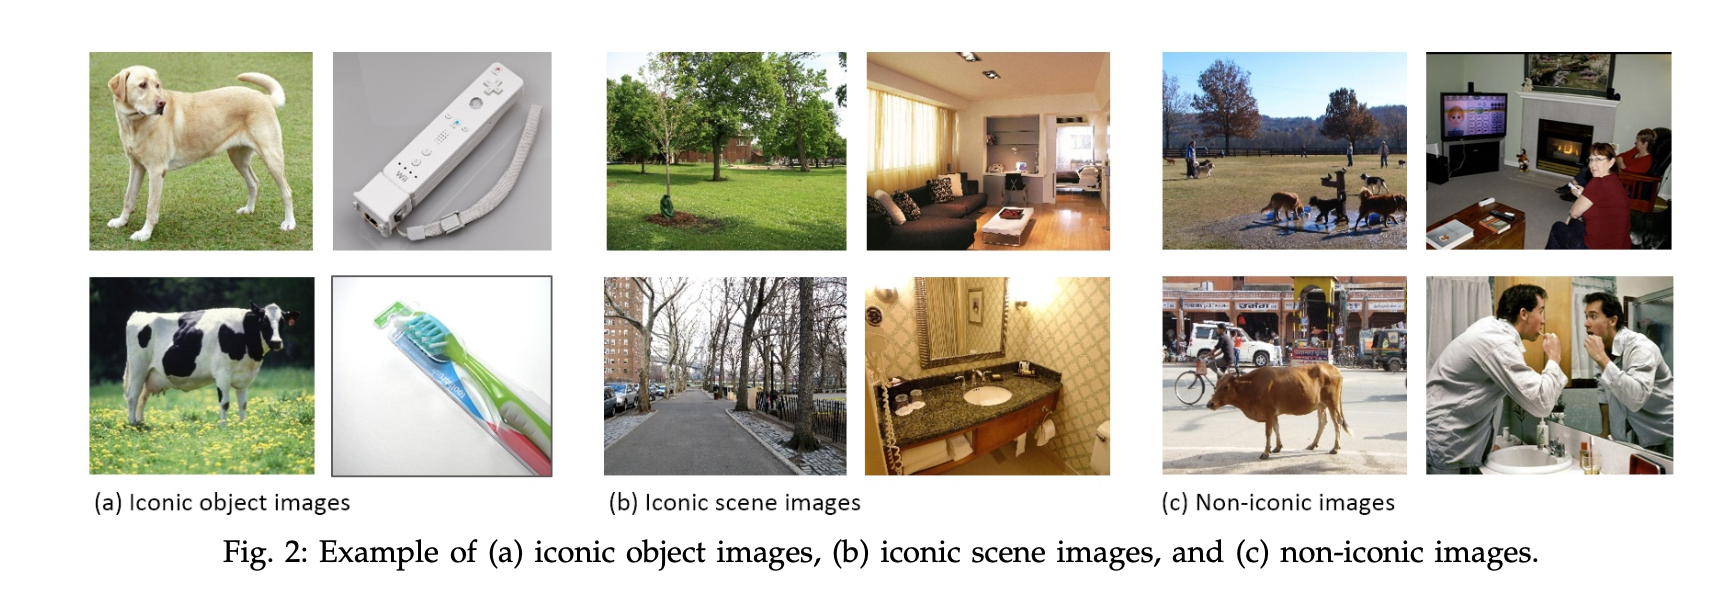
\includegraphics[width=1\linewidth]{figures/02-01/2.1 imagetype} 

}

\caption{Type of images \citep{mccoco}.}\label{fig:imagetype}
\end{figure}

Images are collected through two strategies, firstly images from Flickr which contains photos uploaded by amateur photographer with keywords are collected. Secondly, researchers will search for pairwise combination of object categories like ``dog + car'' to gather more non-iconic images and images with rich contextual relationships.\citep{mccoco}

Due to the the scale of the dataset and the high cost of the annotation process, the design of a high quality annotation pipeline with efficient cost is a difficult task.
The annotation pipeline in Fig \ref{fig:cocoannotation} for COCO is splitted into three primary tasks: 1. category labeling, 2.instance spotting, and 3. instance segmenting.\citep{mccoco}



\begin{figure}

{\centering 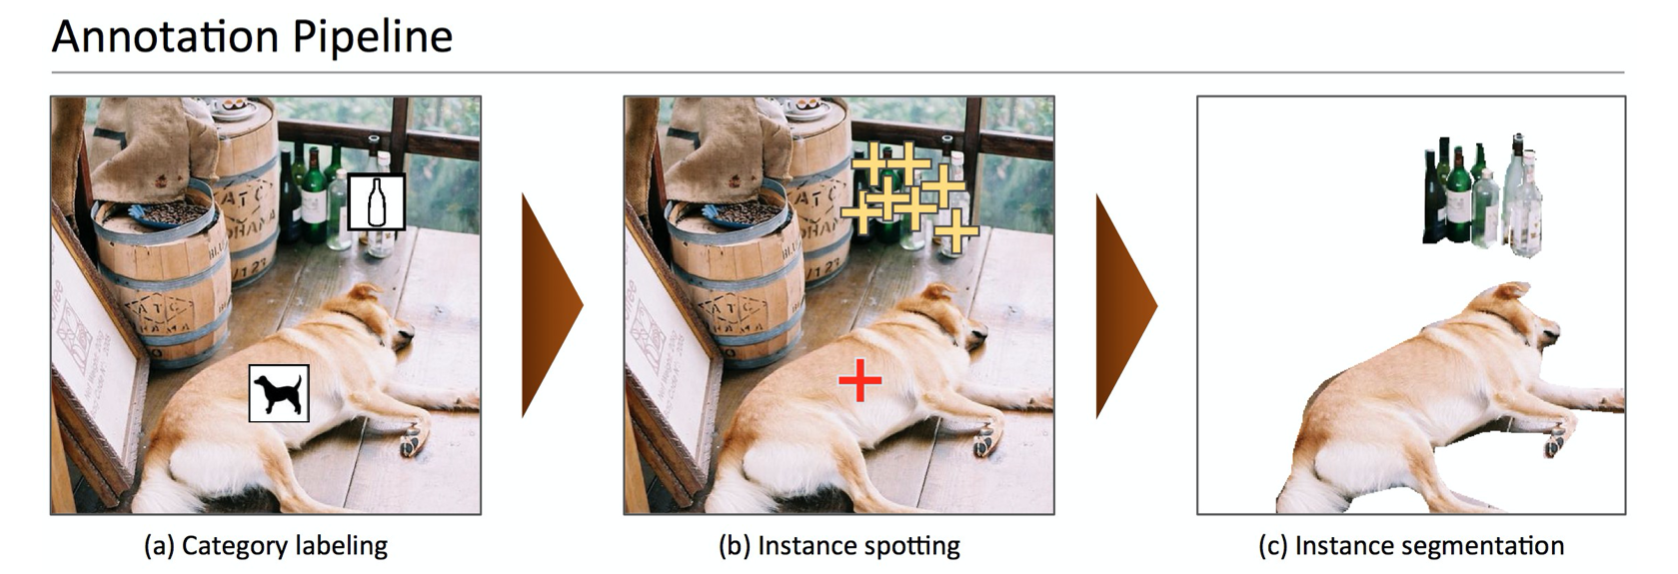
\includegraphics[width=1\linewidth]{figures/02-01/2.1 annotation pipeline} 

}

\caption{Annotation pipeline for COCO \citep{mccoco}.}\label{fig:cocoannotation}
\end{figure}

As we can see in the Fig \ref{fig:cocoannotation}, object categories in each image will be determined in the first step. Due to the large number of Datasets and categories, they used a hierarchical approach instead of doing binary classification for each category. All the 91 categories have divided into 11 super-categories.The worker will examine the existence of a single instance for a given super-category.
Workers will only label one instance for each super-categories with an category's icon.\citep{mccoco} For each image, 8 workers were asked to label it.This hierarchical approach has helped to reduce the time for labeling. However, the first phase still took ∼20k worker hours to complete.\citep{mccoco}

In the next step, all instances of the object categories in an image were labeled, at most 10 instances of a given category per image will be labeled by each worker. In both instance spotting and instance segmenting steps, the location of the instance found by a worker in the previous stage can be seen by the current worker. Each image was labeled by 8 workers for a total of ∼10k worker hours.\citep{mccoco}

In the final segmenting stage, each object instance is segmented, the segmentation for other instances and the specification of the object instance by a worker in the previous stage will also shown to the worker.Segmenting 2.5 Mio object instances is an extremely time consuming task which requires over 22 worker hours per 1,000 segmentations.To minimize cost and improve the quality of segmentation, all workers are required to complete a training task for each object category.
In roder to ensure a better quality, an explicit verification step on each segmented instance was performed.

\hypertarget{comparison-with-other-datasets}{%
\subsubsection{Comparison with other Datasets}\label{comparison-with-other-datasets}}

In recent years, researchers have developed several pre-trained datasets and benchmarks which helped the developemnt of Algorithms for CV.
Each of these datasets varies significantly in size, list of labeled categories and types of images.
In the previos part we also introduced the different research main focus of some Datasets like ImageNet \citep{deng2009imagenet}, PASCAL VOC \citep{pascalvoc} and SUN \citep{sun}
ImageNe containing millions of images has enabled breakthroughs in both object classification and detection research using a new class of deep learning algorithms. It was created to capture a large number of object categories, many of which are fine-grained. SUN focuses on labeling scene types and the objects that commonly occur in them. Finally, PASCAL VOC's primary application is object detection in natural images. MS COCO is designed for the detection and segmentation of objects occurring in their natural context.\citep{mccoco}

With the help of Fig \ref{fig:cococomparison}, we could compare COCO with ImageNet PASCAL VOC and SUN from different aspects.\citep{mccoco}



\begin{figure}

{\centering 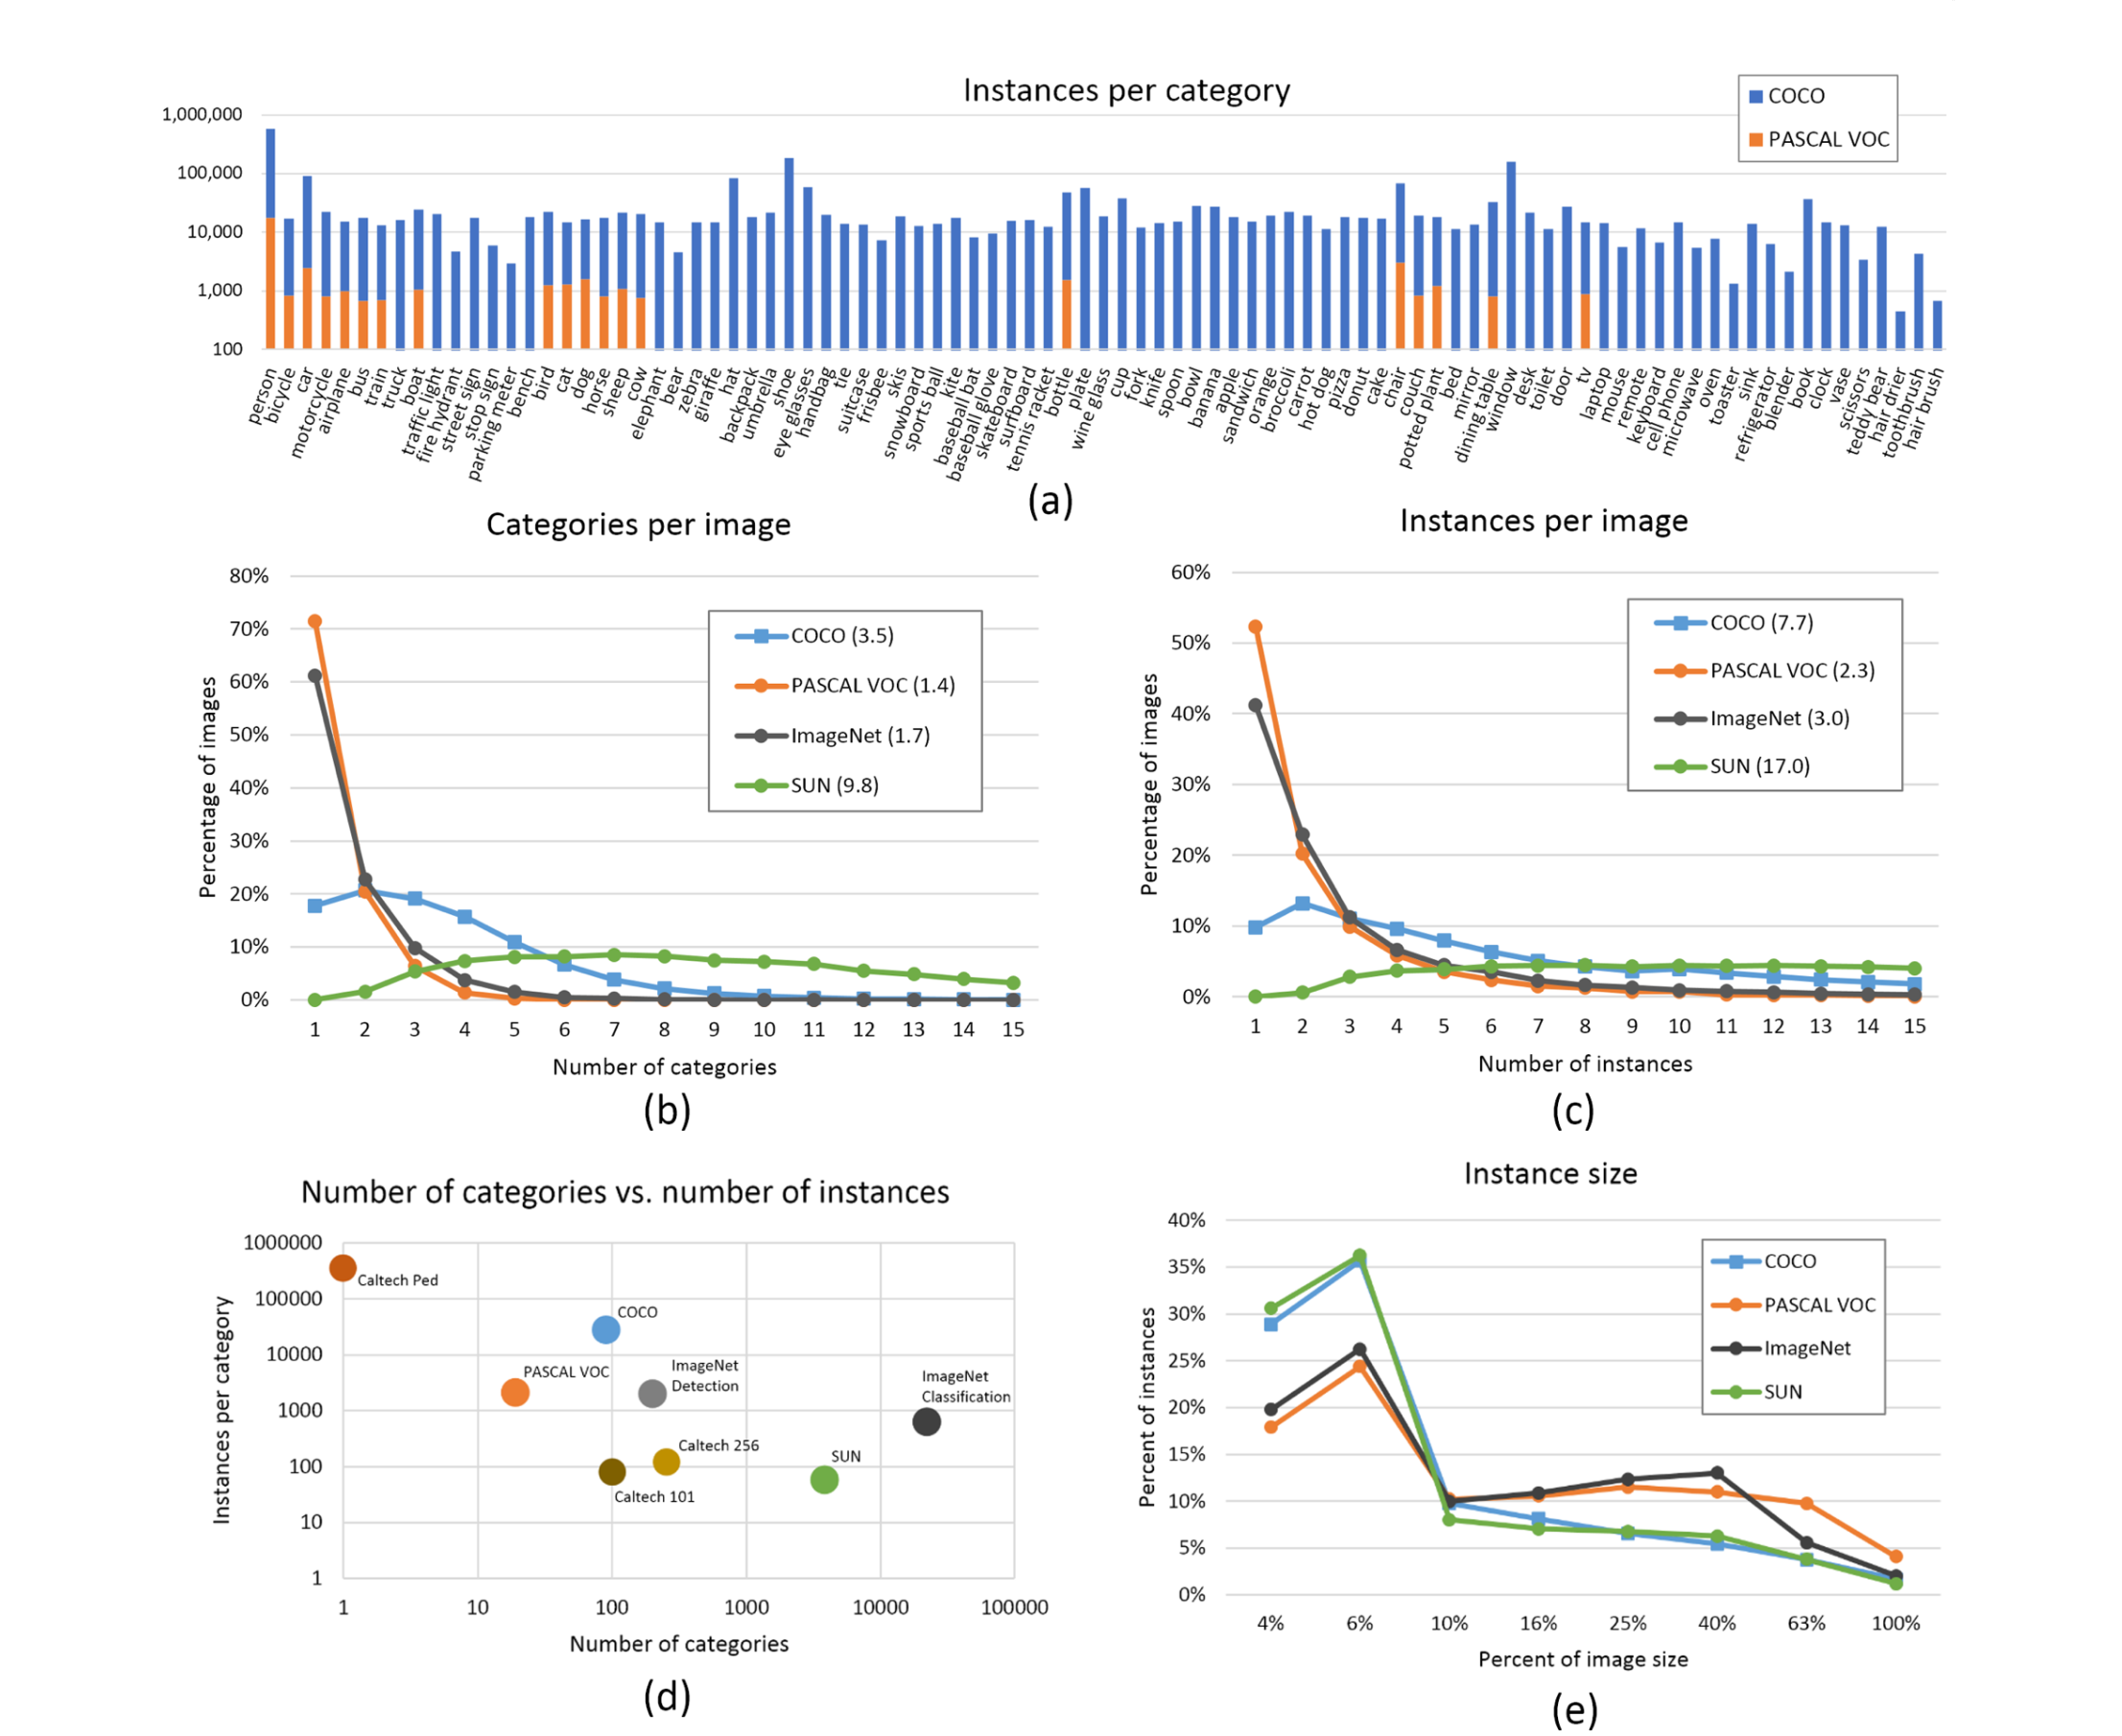
\includegraphics[width=1\linewidth]{figures/02-01/2.1 coco comparison} 

}

\caption{Comparison COCO with other PASCAL VOC, SUN and ImageNet \citep{mccoco}.}\label{fig:cococomparison}
\end{figure}

The number of instances per category for all 91 categories for COCO and PASCAL VOC is shown in (a). Compare to PASCAL VOC, COCO has both more categories and more instances per categories.The number of object categories and the number of instances per category for all the datasets is shown in (d). MS COCO has fewer categories than ImageNet and SUN, but it has the most instances per category among all the dataset, which from the hypothesis of researchers might be useful for learning complex models capable of precise localization.\citep{mccoco}
(b,c) show the number of annotated categories and annotated instances per image for MS COCO, ImageNet Detection, PASCAL VOC and SUN (average number of categories and instances are shown in parentheses). On average COCO contains 3.5 categories and 7.7 instances per image. ImageNet and PASCAL VOC both have less than 2 categories and 3 instances per image on average. SUN dataset has the most contextual information, 9,8 categories and 17 instances per image.
(e) is the distribution of instance sizes for the MS COCO, ImageNet Detection, PASCAL VOC and SUN dataset.\citep{mccoco}

\hypertarget{discussion}{%
\subsubsection{Discussion}\label{discussion}}

COCO is a new large scale data set for detecting and segmenting objects found in everyday life, with the aim of the state-of-the-art in object recognition and scene understanding. It focuses on non-iconic images of objects in natural environments and contains rich contextual information with many objects present per image. COCO is typical vision datasets, which are labor intensive and costly to create.
With the vast cost and over 70,000 worker hours, 2.5 Mio instances were annotated to drive the advancement of object detection and segmentation algorithms. COCO is a good benchmark for the field of CV.\citep{mccoco}
The COCO Team also shows directions for future. For example ``stuff'' label like ``sky'', ``grass'' and ``street'' etc, may also be included in the dataset since ``stuff'' categories provide significant contextual information for the object detection.

\hypertarget{models-for-image-captioning}{%
\subsection{Models for Image captioning}\label{models-for-image-captioning}}

The image captioning task generalizes describe the visual content of an image in natural language, so it requires an algorithm to understand and model the relationships between visual and textual elements, and to generate a sequence of output words.\citep{cornia2020m2}
In the last few years, collections of methods have been proposed for image captioning. Earlier approaches based on generations pf simple templates, which contains the output produced from the object detector or attribute predictor. \citep{Socher10connectingmodalities}, \citep{5487377}.
With the sequential nature of language, most research on image captioning has focused on deep learning techniques,especially using Recurrent Neural Network models (RNNs)\citep{vinyals},\citep{karpthy1} or LSTMs. Mostly, RNNs are used as languages models, and visual information and sequence generation will be encoded from the output of a CNN. With the aim of modelling the relationships between image regions, words, graph convolution neural network in the image encoding phase \citep{yao1} or single-layer attention mechanisms \citep{xu1} on the image encoding side have been proposed to incorporate more semantic and spatial relationships between objects.
RNN-based-models are widely adopted, however, the model has its limitation on representation power and sequential nature.\citep{cornia2020m2}
Recently, new fully-attentive models, in which the use of self-attention has replaced the recurrence,have been proposed. New approaches apply the Transformer models \citep{NIPS2017_3f5ee243} and BERT \citep{devlin-etal-2019-bert} models to image captioning tasks.
Transformer consists of an encoder with a stack of self-attention and feed-forward layers, and a decoder which uses self-attention on words and cross-attention over the output of the last encoder layer.\citep{cornia2020m2}. In some Transformer based approaches, a Transformer-like encoder was paired with an LSTM decoder. While the aforementioned approaches have exploited the original Transformer architecture.
For example Herdade \emph{et al}. \citep{HerdadeKBS19} proposed Transformer architecture for image captioning with the focus on geometric relations between input objects at the same time. Specially,an additional geometric weight between object pairs which is used to scale attention weights are computed. Similarly, an extension of the attention operator in which the final attended information is weighted by a gate guided by the context was introduced by Huang \emph{et al}. \citep{huang1},\citep{cornia2020m2}.

\hypertarget{meshed-memory-transformer-for-image-captioning-m2}{%
\subsection{\texorpdfstring{Meshed-Memory Transformer for Image Captioning (\(M^2\))}{Meshed-Memory Transformer for Image Captioning (M\^{}2)}}\label{meshed-memory-transformer-for-image-captioning-m2}}

Although Transformer-based architectures have been widely implemented in sequence modeling tasks like machine translation and language understanding. However, its applicability for multi-modal tasks like image captioning is still largely under-explored. \citep{cornia2020m2}



\begin{figure}

{\centering 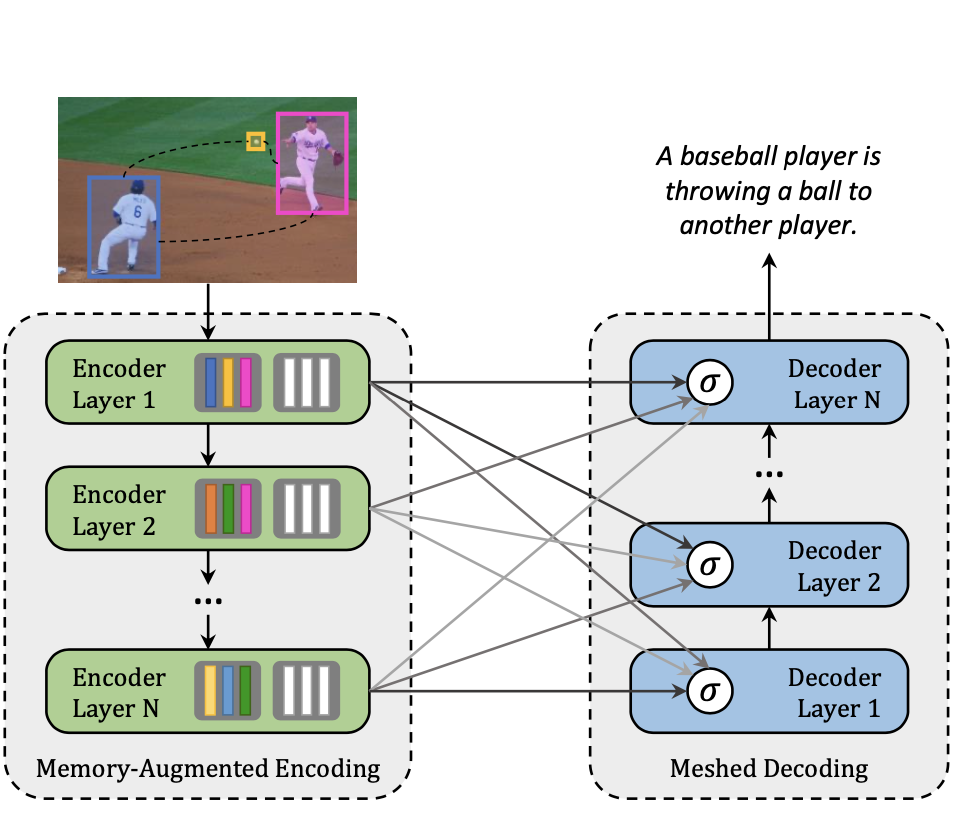
\includegraphics[width=1\linewidth]{figures/02-01/2.2 m2arc1} 

}

\caption{\(M^2\) Transformer \citep{cornia2020m2}.}\label{fig:m2arc1}
\end{figure}

A novel fully-attentive approach called Meshed-Memory Transformer for Image Captioning (\(M^2\)) for image captioning is proposed by Marcella \emph{et al}\citep{cornia2020m2} with the aim of improving the design of both the image encoder and the language decoder. Compare to all previous image captioning models, \(M^2\) ( see Fig. \ref{fig:m2arc1} has two new novelties, the encoder encodes a multi-level representation of the relationships between image regions with respect to low-level and high-level relations, a priori knowledge can be learned and modeled by using persistent memory vectors. The multi-layer architecture exploits both low- and high-level visual relationships through a learned gating mechanism, which compute the weight at each level, therefore, a mesh-like connectivity between encoder and decoder layers is created for sentence generation process.\citep{cornia2020m2}

\hypertarget{m2-transformer-architecture}{%
\subsubsection{\texorpdfstring{\(M^2\) Transformer Architecture}{M\^{}2 Transformer Architecture}}\label{m2-transformer-architecture}}



\begin{figure}

{\centering 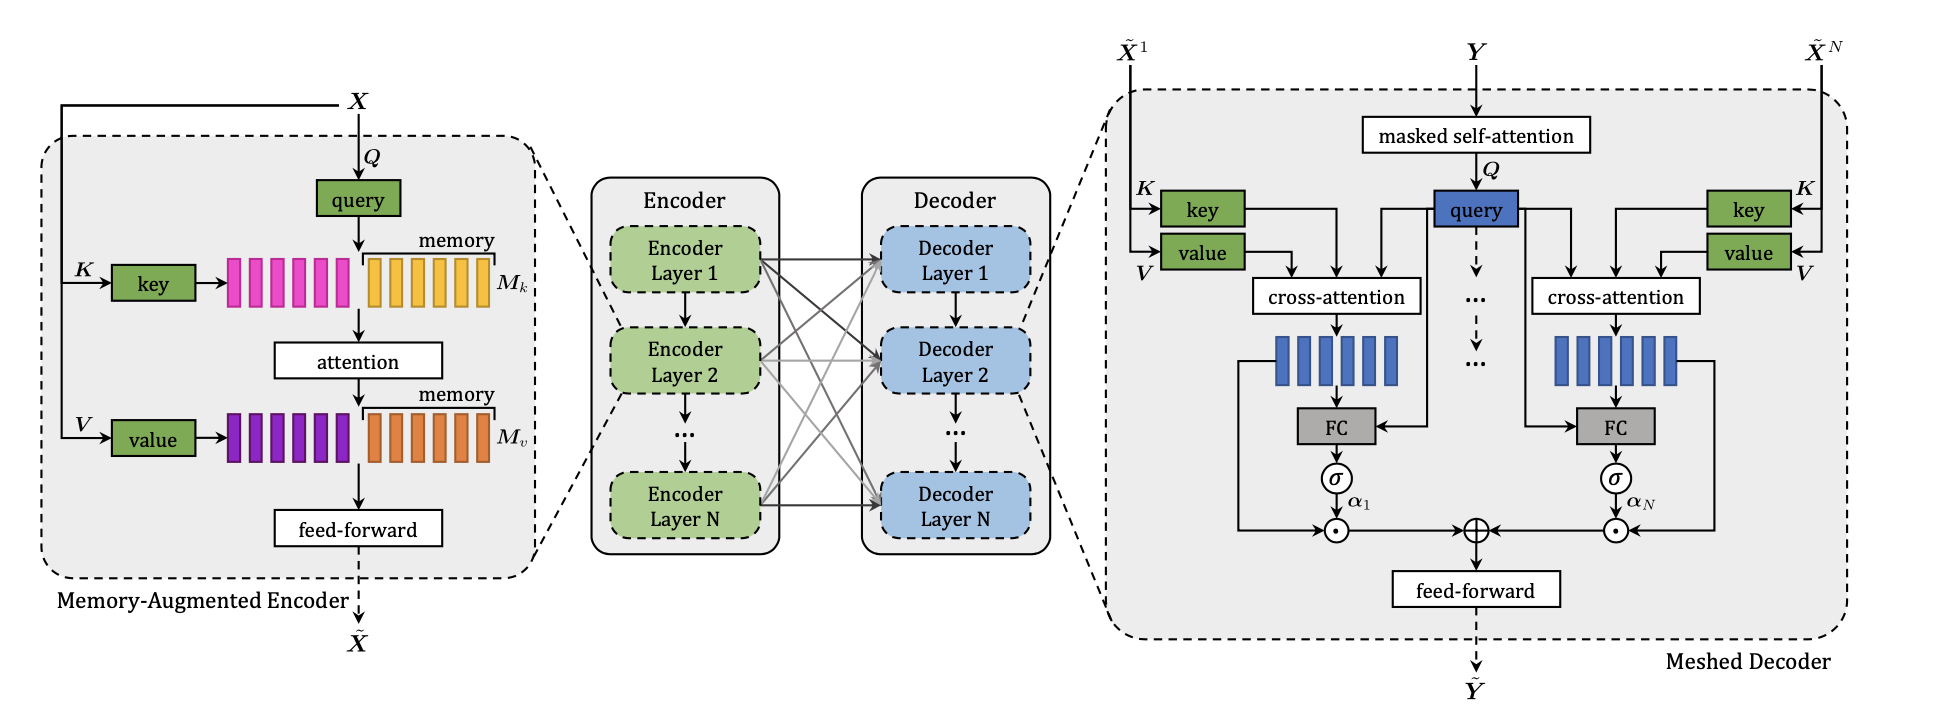
\includegraphics[width=1\linewidth]{figures/02-01/2.1 m2} 

}

\caption{\(M^2\) Transformer Architecture \citep{cornia2020m2}.}\label{fig:m2arc2}
\end{figure}

Fig \ref{fig:m2arc2} shows the detailed architecture of \(M^2\) Transformer. \(M^2\) Transformer can be divided into Encoder (left) module and Decoder (right) module, both module has multiple layers. Given the input Image region \(X\), it go through the Attention and feed forward layer. The relationship between image regions with a priori knowledge will be encoded in each encoding layer, the output of each encoding layers will be read by decoding layers to generate the caption for image word by word.\citep{cornia2020m2}

All interactions between word and image-level features of the input image \(X\) are modeled by using scaled dot-product attention. Attention operates on vectors of queries \(Q\), keys \(K\) and values \(V\) , and takes a weighted sum of value vectors according to a similarity distribution between query and key vectors.
Attention can be defined as follows \citep{cornia2020m2}:

\begin{equation}
Attention(Q, K, V) = softmax(\frac{QK^T}{\sqrt{d}}) V
\label{eq:binom}
\end{equation}

where \(Q\) is a matrix of \(n_q\) query vectors, \(K\) and \(V\) both contain \(n_k\) keys and values, all the vectors has the same dimensionality, and \(d\) is a scaling factor.

\hypertarget{memory-augmented-encoder}{%
\paragraph{Memory-Augmented Encoder}\label{memory-augmented-encoder}}

For the given image region \(X\) , attention can be used to obtain a permutation in- variant encoding of \(X\) through the self-attention operations, the operator from the Transformer can be defined as follows \citep{cornia2020m2}:

\begin{equation}
S(X) = Attention(W_q X, W_k X, W_vX)
\end{equation}

In this case, queries, keys, and values are linear projections of the input features,\(W_q\), \(W_k\), \(W_v\) are learnable weights, they depend solely on the pairwise similarities between linear projections of the input set X. The self-attention operator encodes the pairwise relationships inside the input.
But self-attention also has its limitation: a prior knowledge on relationships between image regions can not be modelled.
To overcome the limitation, Marcella \emph{et al}\citep{cornia2020m2} introduce \textbf{Memory-Augmented Attention} operator by extending the keys and values with additional prior information,which does not depend on image region \(X\).
The additional keys and values are initialized as plain learnable vectors which can be directly updated via SGD.
The operator can be defined as \citep{cornia2020m2}:

\begin{align}
M_{mem}(X) &=  Attention(W_qX, K, V ) \notag \\
K &=  [W_kX, M_k]\notag \\
V &= [W_vX, M_v]
\end{align}

\(M_k\) and \(M_v\) are learnable matrices, with \(n_m\) rows. {[}·,·{]} indicates concatenation. The additional keys and value could help to retrieve a priori knowledge from Input while remaining the quries unchanged.\citep{cornia2020m2}

For the \textbf{Encoding Layer}, Memory-augmented operator is d into a Transformer-like layer, the output applied to position-wise feed-forward layer \citep{cornia2020m2}:

\begin{equation}
F(X)_i= U\sigma(V X_i + b) + c;
\end{equation}

\(X_i\) indicates the \(i\)-th vector of the input set, and \(F(X)_i\) the \(i\)-th vector of the output. Also, \(\sigma(·)\) is the ReLU activation function, \(V\) and \(U\) are learnable weight matrices, \(b\) and \(c\) are bias terms.\citep{cornia2020m2}

Each components will be included in a residual connection and a layer norm operation. The complete definition of an encoding layer can be finally written as \citep{cornia2020m2}:

\begin{align}
Z &= AddNorm(M_{mem}(X))\notag \\
\tilde{X}&=AddNorm(F(Z))
\end{align}

Finally the \textbf{Full Encoder} has multiple encoding layers in sequence, therefore the \(i\)-th layer uses the output set computed by layer \(i − 1\), higher encoding Layers can exploit and refine relationships identified by previous layers, \(N\) encoding layers will produce the output \(\tilde{X} = (\tilde{X}^1 \dots \tilde{X}^n)\).\citep{cornia2020m2}

\hypertarget{meshed-decoder}{%
\paragraph{Meshed Decoder}\label{meshed-decoder}}

The decoder depends on both previously generated words and image region encodings.
\textbf{Meshed Cross-Attention} can take the advantage of all the encoding layers to generate sentences for the image. On the right side of the Fig \ref{fig:m2arc2} shows the structure of the Meshed Decoder. The input sequence vector \(Y\) and the output from all encoding layers \(\tilde{X}\) are connected by Meshed Attention operator gated through cross-attentions. The meshed attention operator can be formally defined as \citep{cornia2020m2}:

\begin{equation}
M_{mesh}(\tilde{X}, Y) =\sum_{i = 1}^{N}\alpha_i C(\tilde{X^i}, Y)
\end{equation}

\(C(·, ·)\) stands for the encoder-decoder cross-attention, it could be defined with queries from decoder and the keys and values from encoder.\citep{cornia2020m2}

\begin{equation}
C(\tilde{X^i}, Y) = Attention(W_q Y, W_k \tilde{X^i}, W_v \tilde{X^i})
\end{equation}

\(\alpha_i\) is a matrix of weights same size as the cross-attention results, \(\alpha_i\) models both single contribution of each encoding layer and the relative importance between different layers.\citep{cornia2020m2}

\begin{equation}
\alpha_i = \sigma(W_i [Y,C(\tilde{X^i}, Y)]+ b_i)
\end{equation}

The {[}·,·{]} indicates concatenation and \(\sigma\) is the sigmoid activation function, \(W_i\) is a weight matrix, and \(b_i\) is a learnable bias vector.\citep{cornia2020m2}

In decoding layers the prediction of a word should only depend on the word generated previously, so the decoder layer comprises a masked self- attention operation, the operator build connection between queries derived from the \(t\)-th element of its input sequence Y with keys and values from left sub-sequence,i.e.~\(Y_{≤t}\).

Simlilar as the Encoding layer, the decoder layer also contains a position-wise feed-forward layer, so the decoder layer can be finally defined as \citep{cornia2020m2}:

\begin{align}
Z &= AddNorm(M_{mesh}(X,AddNorm(S_{mask}(Y ))) \notag \\
\tilde{Y} &= AddNorm(F(Z)),
\end{align}

\(S_{mask}\) indicates a masked self-attention over time.\citep{cornia2020m2}
Decoder with multiple decoder layers, takes the input word vectors and the \(t\)-th element of its output sequence to make the prediction of a word for \(t + 1\), conditioned on th \(Y_{≤t}\). Finally the decoder takes a linear projection and a softmax operation, which encodes a probability over words in the dictionary.\citep{cornia2020m2}

\hypertarget{comparison-with-other-models-on-coco-datasets}{%
\paragraph{Comparison with other models on COCO Datasets}\label{comparison-with-other-models-on-coco-datasets}}

The \(M^2\) Transformer was evaluated on COCO \citep{mccoco}. COCO is the most commonly used Test dataset for image captioning. In stead of using the original COCO datsets, Marcella \emph{et al}\citep{cornia2020m2} follows the split of COCO provided by Karpathy \emph{et al} \citep{karpthy1}. Karpathy uses 5000 images for validation, 5000 images for testing and the rest for training.

For model evaluation and comparison, standard captioning metrics like BLEU \citep{papineni-etal-2002-bleu}, METEOR \citep{meteor}, ROUGE \citep{lin-2004-rouge}, CIDEr \citep{cider}, and SPICE \citep{spice} which have been introduced in the second chapter are used.



\begin{figure}

{\centering 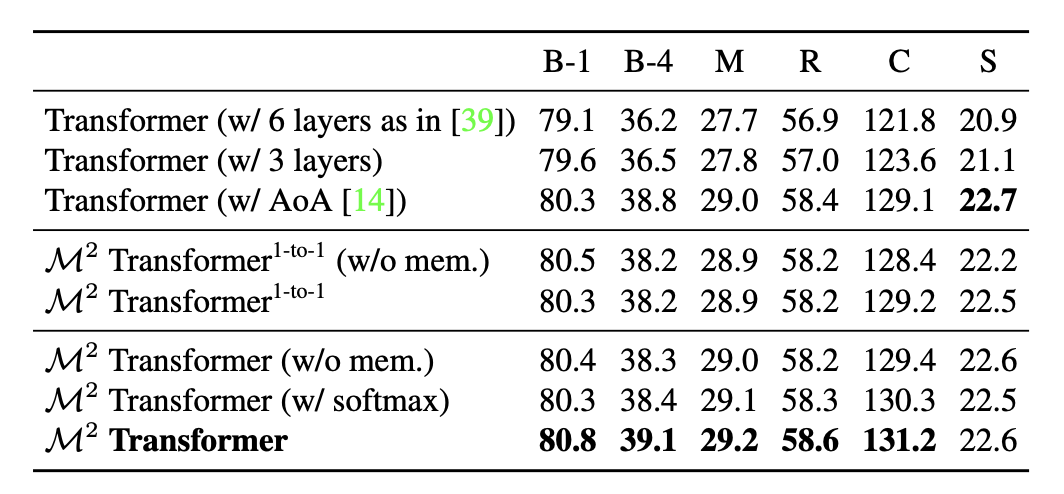
\includegraphics[width=1\linewidth]{figures/02-01/02-02 compare1} 

}

\caption{Comparison with Transformer-based alternatives \citep{cornia2020m2}}\label{fig:compare1}
\end{figure}

Transformer model in original configuration with six layers has been applied to captioning, researchers speculated that specific architectures are required for captioning, so variations of the original Transformer are compared with \(M^2\) Transformer. Other Variations are Transformer with three layers and ``Attention on Attention'' (AoA) approach \citep{huang1} to the attentive layers, both in the encoder and in the decoder. \citep{cornia2020m2}
The second part intends to evaluate the importance of the meshed connections between encoder and decoder layers. \(M^2\) Transformer (1 to 1) is a reduced version of original \(M^2\) Transformer, in which one encoder layer only connect to one corresponding decoder layer instead of connect to all the decoding layers.
As we can see from the Fig \ref{fig:compare1}, the original Transformer has 121.8 CIDEr, compare with it, the reduced version of \(M^2\) Transformer, we can see the improvement already (129.2 CIDEr). With the respect to meshed connectivity, which help to exploit relationships encoded at all layers and weights them with a sigmoid gating, we could observe better improvement in CIDEr from 129.2 to 131.2. Also the role of mem- ory vectors and the softmax gating schema for \(M^2\) Transformer are also included in the table. Without the memory vector lead to the recution of the performance of nearly 1 CIDEr in both reduced \(M^2\) Transformer and the original \(M^2\) Transformer.\citep{cornia2020m2}



\begin{figure}

{\centering 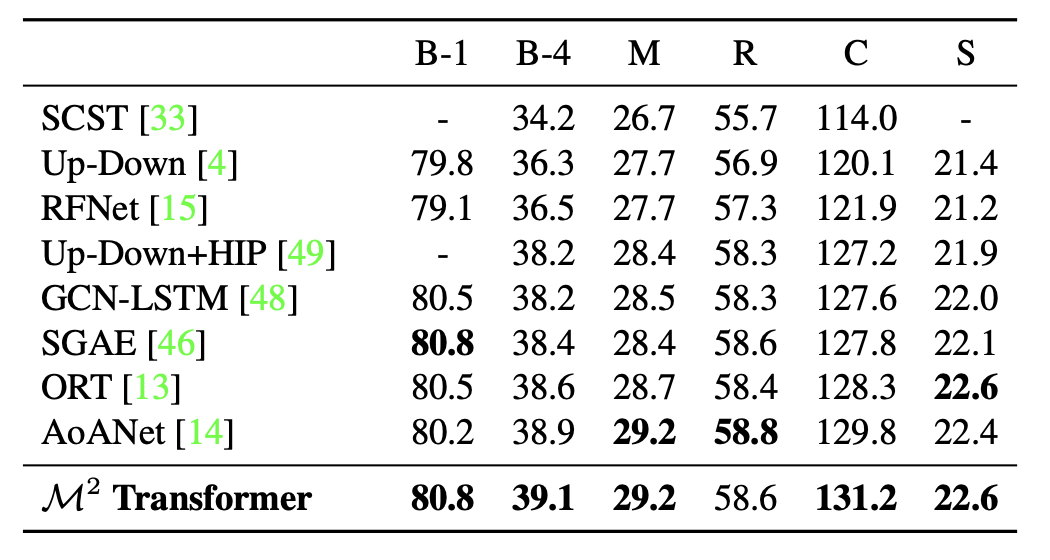
\includegraphics[width=1\linewidth]{figures/02-01/02-02 compare2} 

}

\caption{Comparison with the state of the art on the ``Karpathy'' test split, in single-model setting \citep{cornia2020m2}}\label{fig:compare2}
\end{figure}

Fig \ref{fig:compare2} compares the performance of \(M^2\) Transformer with several recent proposals for image captioning.
SCST \citep{8099614} and Up- Down \citep{8578734}, use attention over the grid of features and attention over regions. RFNet \citep{renet}, which uses a recurrent fusion network to merge different CNN features; GCN-LSTM \citep{GCN-LSTM} uses a Graph CNN to exploit pairwise relationships between image regions; SGAE \citep{Yang_2019_CVPR} uses instead auto-encoding scene graphs. The original AoANet \citep{huang1} approach uses attention on attention for encoding image regions and an LSTM language model. Finally, the ORT \citep{HerdadeKBS19} uses a plain Transformer and weights attention scores in the region encoder with pairwise distances between detections \citep{cornia2020m2}.

In Fig \ref{fig:compare2}, the \(M^2\) Transformer exceeds all other models on BLEU-4, METEOR,CIDEr. The performance of \(M^2\) Transformer was very close and competitive with SGAE on BLEU-1 and with ORT on SPICE.



\begin{figure}

{\centering 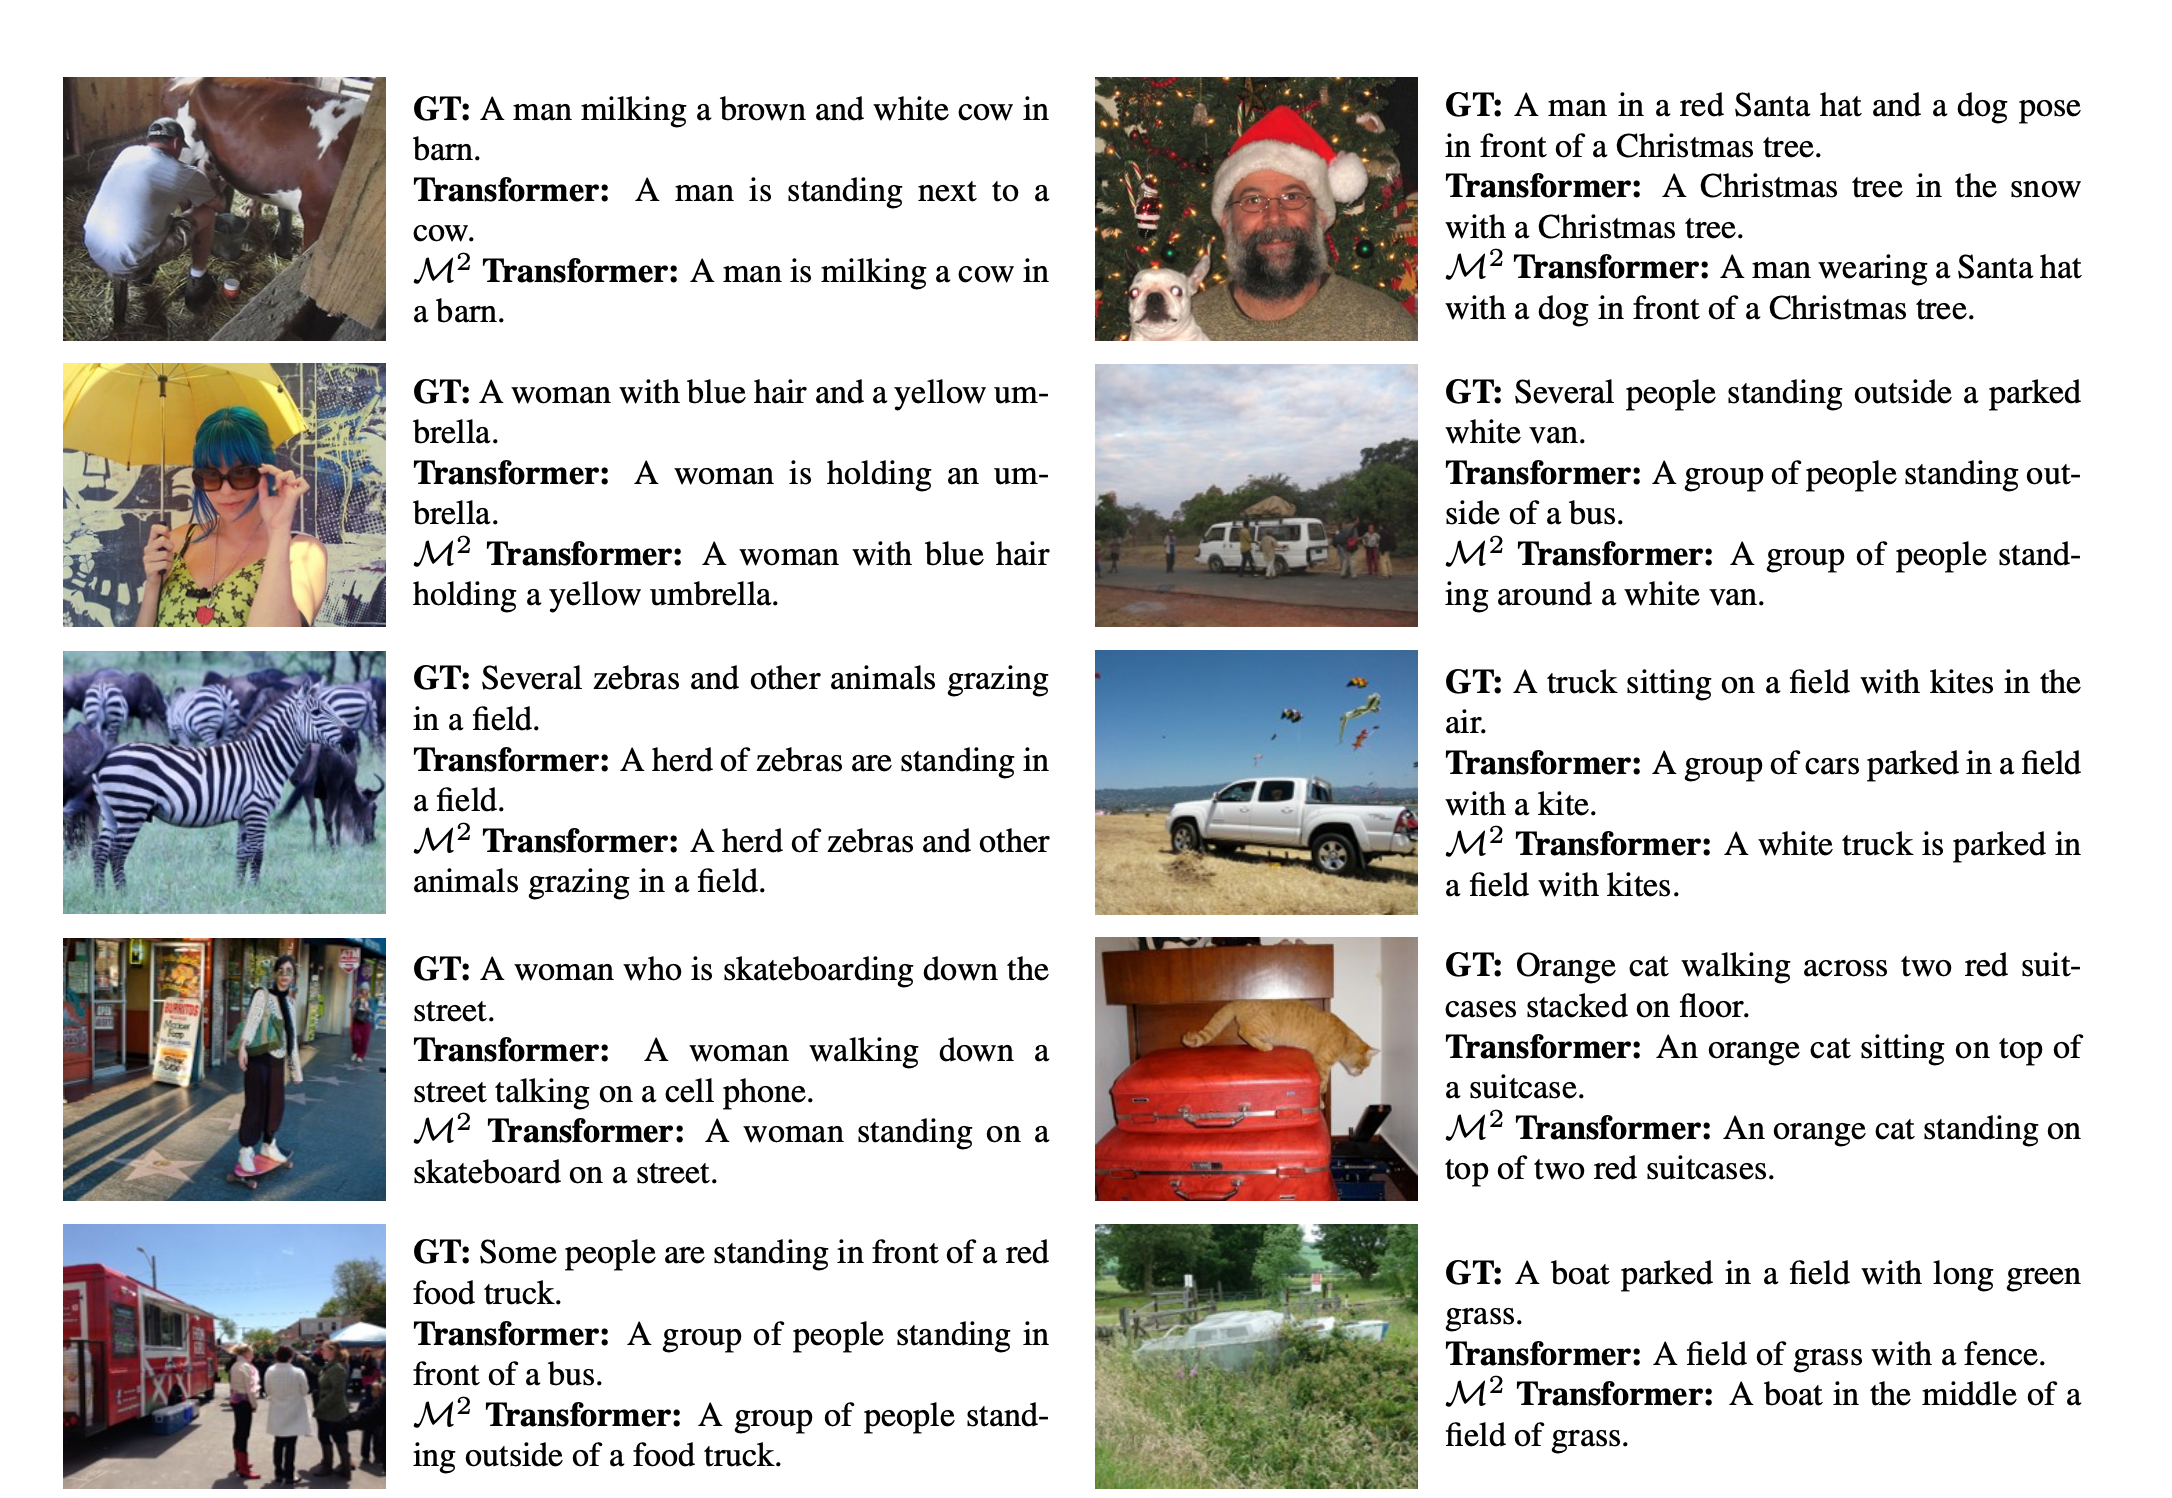
\includegraphics[width=1\linewidth]{figures/02-01/02-02 example2} 

}

\caption{"Examples of captions generated by M\^{}2\$ Transformer and the original Transformer model, as well as the corresponding ground-truths \citep{cornia2020m2}}\label{fig:example2}
\end{figure}

The Fig \ref{fig:example2} shows some examples of captions generated by \(M^2\) Transformer and the original Transformer model, as well as the corresponding ground-truths. According to the selected examples of captions, \(M^2\) Transformer shows the ability to generate more accurate descriptions of the images, and the approaches could detect the more detailed relationships between image regions.\citep{cornia2020m2}.

The \(M^2\) Transformer is a new Transformer- based architecture for image captioning. It improves the image encoding by learning a multi-level representation of the relationships between image regions while exploiting a priori knowledge from each encoding layer, and uses a mesh-like connectivity at decoding stage to exploit low- and high-level features at the language generation steps. The results of model evaluation with COCO shows that, the performance of \(M^2\) Transformer approach surpasses most of the recent approaches and achieves a new state of the art on COCO.\citep{cornia2020m2}.

\hypertarget{c02-02-text2img}{%
\section{Text-2-image}\label{c02-02-text2img}}

\emph{Author:} Karol Urbańczyk

\emph{Supervisor:} Jann Goschenhofer

\begin{itemize}
\tightlist
\item
  introduce the concept in few sentences
\item
  choice of recent break-throughs is subjective, many important ones not mentioned (GAWWN, LAFITE, Make-a-Scene, probably many others)
\end{itemize}

Intention of this chapter is to grasp how the field of text-2-image modelling has been changing over the recent years. We will start with basic concepts that has been around since 2014 and end with the state-of-the-art approaches, as of August 2022. Since the field is developing in a rapid pace, with break-through models being announced every quarter, we are aware this chapter might soon not be fully covering the field. However, we must notice that cutting edge capabilities of these models tend to come from the scale and software engineering tricks. Therefore, we believe that focusing on the core concepts should make this chapter have a universal character.

\hypertarget{seeking-objectivity}{%
\subsection{Seeking objectivity}\label{seeking-objectivity}}

\begin{itemize}
\tightlist
\item
  Objectivity in comparing generated images is very hard to grasp
\item
  However, there are some most common datasets and measures that are being used
\item
  This subchapter will quickly present them
\end{itemize}

\hypertarget{datasets-1}{%
\subsubsection{Datasets}\label{datasets-1}}

\begin{itemize}
\tightlist
\item
  COCO
\item
  CUB
\item
  Oxford 102
\end{itemize}

\hypertarget{measures}{%
\subsubsection{Measures}\label{measures}}

\begin{itemize}
\tightlist
\item
  FID (Frechet Inception Distance)
\item
  IS (Inception Score)
\item
  Human evaluations - photorealism / caption similarity
\end{itemize}

\hypertarget{generative-adversarial-networks}{%
\subsection{Generative Adversarial Networks}\label{generative-adversarial-networks}}

\begin{itemize}
\tightlist
\item
  quick intro focusing on why it is crucial to start from GANs
\end{itemize}

\hypertarget{vanilla-gan-for-image-generation}{%
\subsubsection{Vanilla GAN for Image Generation}\label{vanilla-gan-for-image-generation}}

\begin{itemize}
\tightlist
\item
  intro of GAN
\end{itemize}

\hypertarget{conditioning-on-text}{%
\subsubsection{Conditioning on Text}\label{conditioning-on-text}}

\begin{itemize}
\tightlist
\item
  how to encode the text and use it in the generation process
\item
  show some results
\end{itemize}

\hypertarget{stacking-generators}{%
\subsubsection{Stacking generators}\label{stacking-generators}}

\begin{itemize}
\tightlist
\item
  intro of StackGAN, show some results
\end{itemize}

\hypertarget{is-attention-all-you-need}{%
\subsubsection{Is attention all you need?}\label{is-attention-all-you-need}}

\begin{itemize}
\tightlist
\item
  intro of AttGAN, show some results
\end{itemize}

\hypertarget{variational-autoencoder}{%
\subsubsection{Variational Autoencoder}\label{variational-autoencoder}}

\begin{itemize}
\tightlist
\item
  Introducing the concept of VAE
\item
  How is it helpful in generating images
\end{itemize}

\hypertarget{dall-e-starting-post-gan-era}{%
\subsection{Dall-E starting post-GAN era}\label{dall-e-starting-post-gan-era}}

\begin{itemize}
\tightlist
\item
  Intro: OpenAI, dataset used, not public, etc
\item
  VQ-VAE and dVAE
\item
  Details how it's working. Combining Transformer with VQ-VAE. Training vs inference
\item
  Results and image examples
\end{itemize}

\hypertarget{glide}{%
\subsection{GLIDE}\label{glide}}

\begin{itemize}
\tightlist
\item
  Intro
\item
  Diffusion concept
\item
  details how GLIDE is working
\item
  results / scores
\item
  Limitations / strengths \& weaknesses
\end{itemize}

\hypertarget{dall-e-2}{%
\subsection{Dall-E 2}\label{dall-e-2}}

\begin{itemize}
\tightlist
\item
  Intro (mention PR move)
\item
  details how it is working
\item
  results / scores
\item
  Limitations / strengths \& weaknesses
\end{itemize}

\hypertarget{imagen}{%
\subsection{Imagen}\label{imagen}}

\begin{itemize}
\tightlist
\item
  Intro
\item
  details how it is working
\item
  results / scores
\item
  Limitations / strengths \& weaknesses
\end{itemize}

\hypertarget{parti}{%
\subsection{Parti}\label{parti}}

\begin{itemize}
\tightlist
\item
  Intro
\item
  details how it is working
\item
  results / scores
\item
  Limitations / strengths \& weaknesses
\end{itemize}

\hypertarget{open-source-community}{%
\subsection{Open-Source Community}\label{open-source-community}}

\begin{itemize}
\tightlist
\item
  Although most of the recent work comes from OpenAI and Google, there are very interesting directions taken by the open community
\item
  Mentioning the models and quickly what is happening. VQGAN+CLIP, Latent Diffusion models for sure
\item
  Maybe some links for the reader to play with?
\end{itemize}

\hypertarget{discussion-1}{%
\subsection{Discussion}\label{discussion-1}}

Mention the following points and why they matter

\begin{itemize}
\tightlist
\item
  potential business use cases
\item
  open vs closed-source (mention dall-e mini)
\item
  copyrights
\item
  biases
\end{itemize}

\hypertarget{c02-03-img-support-text}{%
\section{Images supporting Language Models}\label{c02-03-img-support-text}}

\emph{Author:} Giacomo Loss

\emph{Supervisor:} Matthias Aßenmacher

\hypertarget{words-in-non-symbolic-contexts}{%
\subsection{Words In (Non-Symbolic) Contexts}\label{words-in-non-symbolic-contexts}}

Imagine you were alone in a foreign country, you could not speak the language and the only resource you had were a dictionary in the foreign language. You see a word written on a sign but you cannot understand its meaning. What could you do? One idea would be do open the dictionary and look the word up. The problem is that the word is defined by using other words in the foreign language. As a second step you would thus look these new words up and continue like that in further steps to the ``infinity and beyond'' (cit. Buzz Lightyear). But even after looking every single word in the dictionary up, you would still not be able to understand the meaning of the word written on the sign. If on that sign, next to the unknown word, something else was instead depicted, for example an image of a fork and a knife, you might speculate that the word indicates something which has to do with food, like a restaurant. And this without explicitly knowing the meaning of the word. This example is inspired by the work of Stevan Harnad, which formulated at the beginning of the 90's the so called \emph{Symbol Grounding Problem} (\citet{harnad1990symbol}). It asserts that it is not possible to understand the meaning (semantics) of a word by just looking at other words because words are essentially meaningless symbols. It is possible to understand the meaning only if the word is put in a context, a perceptual space, other than that of written language: the word must be \emph{grounded} in non-symbolic representations, like images, for example. Over the past 10 years there has been a whopping development of distributional semantic models (DSMs, henceforth), especially after the Word2vec (\citet{mikolov2013efficient}) revolution. This family of models assumes that the meaning of words and sentences can be inferred by the ``distribution'' of those words and sentences within a text corpus (the \emph{Distributional Hypothesis} formulated by \citet{harris1954distributional}). But the \emph{Symbol Grounding Problem} mentioned earlier suggests that DSMs do not resemble the way words are learned by humans, which is in multimodal perceptual contexts. For these reasons, models have been developed with the goal to integrate further modalities (like visual ones) in pure language models, assuming that grounding words and sentences in other perceptual contexts should lead to a better understanding of their semantics and, as a result, to better performance in pure language tasks.

The focus of this subchapter are models which empower pure language models with visual modalities in form of images: their goal is to obtain better semantic representations (in form of embedding vectors) of words. First, a quick recap of the main pure language models will be provided. After that, the historical evolution of the integration of images as visual modalities into pure language models will be discussed: from simple concatenation of textual and visual modalities, to the projection of visual elements in a common grounded space and more recently, the use of Transformers (see figure \ref{fig:img-hist}). Eventually, a comprehensive evaluation of the different models against benchmarks will be carried out.

Again, the focus is on how to employ visual elements to obtain embeddings able to capture the semantics of words. More concrete applications, such as those in the field of machine translation are out of scope and will be only marginally addressed at the end of the subchapter.

\begin{figure}

{\centering 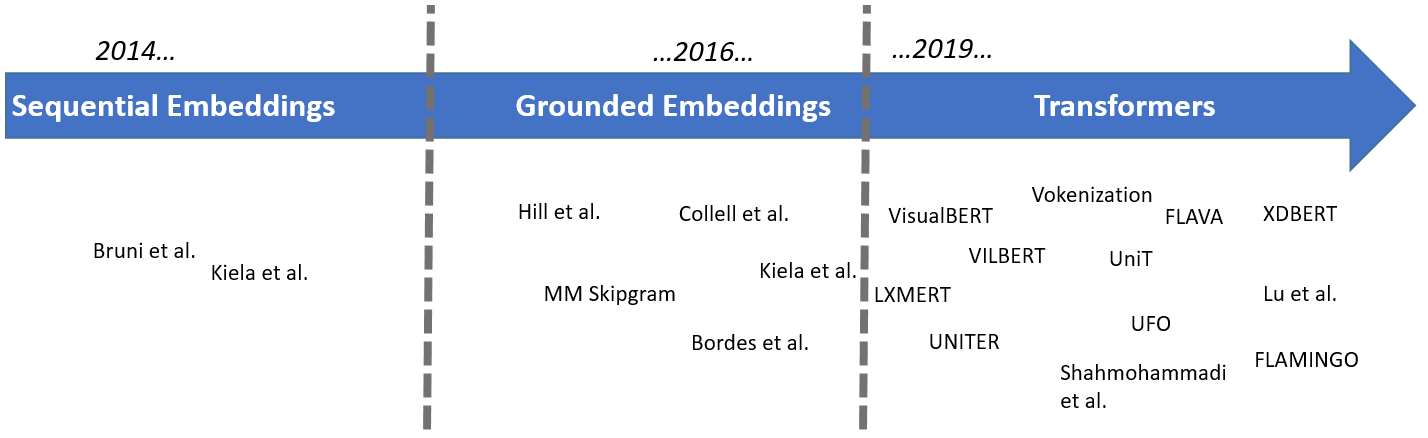
\includegraphics[width=1\linewidth]{figures/02-03-img-support-text/Img-Hist} 

}

\caption{Historical evolution of models which integrate visual information into pure language models. }\label{fig:img-hist}
\end{figure}

\hypertarget{word-embeddings-survival-kit}{%
\subsection{Word-Embeddings: Survival-Kit}\label{word-embeddings-survival-kit}}

In other parts of this books, the most important NLP-models and the latest developments in the field are extensively described. In this section, some information will be provided, which might be helpful to understand some of the aspects discussed in this subchapter. As it may have been inferred in the introduction, the starting point is always a pure language model, namely a model which employs only textual inputs in order to generate word embeddings, which are representations of words in form of numerical vectors.
The most widely used pure language models in the papers presented in this subchapter are the following three:

\begin{itemize}
\tightlist
\item
  \textbf{Skipgram} (Word2vec, \citet{mikolov2013efficient}), where given a target word, the probability of the neighboring (surrounding) words in a pre-defined window has to be maximized. Trainig takes place either through a \emph{hierarchical softmax} or through \emph{negative sampling}, which involves maximizing the probability of words which are real neighbors and minimizing that of words which are not real neighbors (the ``negative samples'')
\item
  \textbf{GloVe} (\citet{pennington2014glove}), which is based on words co-occurrence across the \emph{entire} corpus, with the goal of minimizing the difference between the dot product of the embedding vectors of two words and the logarithm of the number of co-occurrences
\item
  \textbf{BERT} (\citet{devlin2018bert}): two pre-training tasks to obtain word-embeddings:

  \begin{itemize}
  \tightlist
  \item
    Masked Language Modelling (MLM): given a sentence with {[}MASK{]}ed tokens, the goal is to predict these masked tokens
  \item
    Next Sentence Prediction (NSP): given two sentences A and B, the goal is to predict if B follows from A
  \end{itemize}
\end{itemize}

Two additional remarks to conclude this section. First, Skipgram and GloVe generate embeddings which are \emph{``context-free''}: they do not take into account the context in which words occur. On the contrary, BERT is designed to represent words given the context (sentence) in which they occur: we can thus have different embeddings for the same word, depending on the context.
Second, the inputs of these models are \emph{tokens}: with the help of a \emph{tokenizer}, which can be different for different models, the text is split in ``chunks'', called \emph{tokens} (and they are not necessarily single words).

\hypertarget{the-beginning-sequential-multimodal-embeddings}{%
\subsection{The Beginning: Sequential Multimodal Embeddings}\label{the-beginning-sequential-multimodal-embeddings}}

Supposing we add linguistic and visual feature representations related to a particular word, how could we fuse them? One intuitive idea would be to \emph{concatenate} the textual and visual modalities. Let \(V_{text}\) be the textual (vectorial) representation of a word and let \(V_{img}\) be its visual (vectorial) representation, a fused representation \(F\) of a certain word \(w\) might take the following simplified form:

\[F=\gamma(V_{text})\bigoplus(1-\gamma)V_{img}\]

where \(\gamma\) is a tuning parameter which controls the relative contribution of both modalities to the final fused representation. \citet{bruni2014multimodal} propose a model where the meaning of a target word is represented in the form of a semantic vector and all vectors are collected in a \emph{text-based semantic matrix}; textual embeddings are computed based on (transformed) co-occurrence counts of words in a pre-defined window. The starting point to obtain an image-based representation of certain target word is a dataset of labeled images. For each image associated to the target word (which means that the target word is to be found in the image's caption), low-level features called ``local descriptors'' - which incorporate geometric information of specific areas of a certain picture - are extracted and then these descriptors are assigned to clusters (\emph{bags}) of ``visual words''\footnote{See for example \citet{bosch2007image} for more details on this technique, called ``bag-of-visual-words''.}. Afterwards, for each target word, visual word occurrences are summed up together to obtain the occurrence counts related to the target word. These image-based semantic vectors are then transformed and collected in an \emph{image-based semantic matrix}. The two matrices are then concatenated and projected into a common latent multimodal space with a singular value decomposition. Thanks to this process a \emph{textual \textbf{mixed} matrix} and a \emph{visual \textbf{mixed} matrix} are extracted and then combined together according to different fusion strategies to build the multimodal embeddings. In this first, relatively cumbersome (historically motivated) example, the vector representation of an image is obtained with non-trivial features engineering.

In recent years, the use of neural networks has made an ``automatic feature selection'' possible. This is what for example \citet{kiela2014learning} propose, extracting visual features from the first seven layers of a convolutional neural network (proposed by \citet{krizhevsky2012imagenet}) trained on 1.6 million images from the ImageNet database (\citet{deng2009imagenet}), which produces scores for 1,512 object categories. The linguistic part of the model relies on the Skipgram model by \citet{mikolov2013efficient} and consists of 100-dimensional vector representations. The multimodal representation is again obtained by concatenation of both modalities.

\begin{figure}

{\centering 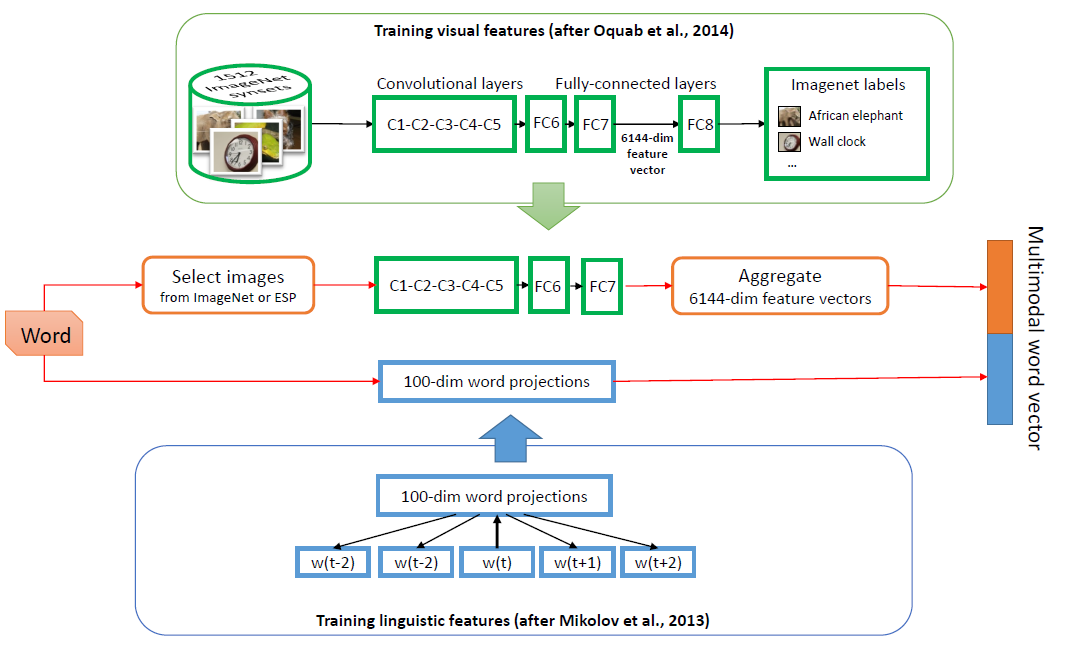
\includegraphics[width=1\linewidth]{figures/02-03-img-support-text/img-kiela2014-01} 

}

\caption{From @kiela2014learning. Textual and visual features vectors are concatenated.}\label{fig:img-kiela2014-01}
\end{figure}

Another notable example of concatenation/sequential combination of textual and visual modalities is the work of \citet{silberer2014learning}: textual and visual modalities are represented by separate vectors of textual and visual attributes. During training, these textual and visual inputs vectors are separately fed to denoising (unimodal) autoencoders, the training objective of which is the reconstruction of a certain corrupted input - e.g.~through masking noise - from a latent representation. Their outputs are then jointly fed to a bimodal autoencoder to be mapped to a multimodal space, on which a softmax layer (classification layer) is added, which allows the architecture to be fine-tuned for different tasks.

\hypertarget{the-grounded-space}{%
\subsection{The Grounded Space}\label{the-grounded-space}}

The aforementioned models assume implicitly a one-to-one correspondence between text and images: a visual representation is extracted only from words which are associated to a concrete image. This is a limitation, for two partially overlapping reasons. One one hand, how can we depict words for which no image is available in our training set? Is it possible to \emph{imagine} visual representations purely from linguistic ones? On the other hand, could we hypothetically find a visual representation for each word? This might be true for concrete words but when it comes to abstract ones, it is not always possible to find suitable visual representations or, said in other terms, many words are not visually grounded. For this reasons, researches have addressed the question: could we map textual and visual elements to a grounded space and design models able to generalize images and words beyond those in the training set? Well, the answer is yes!

\citet{lazaridou2015combining} propose a multimodal Skip-gram architecture where the objective function of a Skip-gram is ``augmented'' with an additional visual objective: \[\frac{1}{T}\sum_{t=1}^{T}\left(\mathcal{L}_{ling}(w_{t})+\mathcal{L}_{vision}(w_{t})\right)\]

where \(\mathcal{L}_{ling}\) is the Skip-gram loss function and \(\mathcal{L}_{vision}\) is the additional visual loss for the target word \(w_{t}\). In particular, \(\mathcal{L}_{vision}\) has the form of a hinge loss, the goal of which is to make the (vectorial) linguistic representation of a certain word more similar to its visual representation:

\[\mathcal{L}_{vision}(w_{t})=-\sum_{w^{'}\sim P_{n}(w)}\left(max(0,\gamma-cos(z_{w_{t}},v_{w_{t}})+cos(z_{w_{t}},v_{w^{'}})\right)\]

where \(v_{w^{'}}\) is a visual representation of a randomly chosen word \(w^{'}\) (drawn from a probability distribution \(P_{n}(w)\)) used as negative sample, \(v_{w_{t}}\) is the corresponding visual vector and \(z_{w_{t}}\) is the target multimodal word representation which has to be learned by the model. It is nothing more than a linear transformation of a word representation \(u_{w_{t}}\): \(z_{w_{t}}=M^{u\rightarrow v}u_{w_{t}}\) and \(M^{u\rightarrow v}\) is a cross-modal mapping matrix from linguistic inputs to a visual representation. It is important to remark that during training, for words which do not have associated images, \(\mathcal{L}_{vision}\) gets set to zero. When this cross-modal mapping matrix is estimated, it is then possible to find a visual representation for new words, which do not have a related image in the training set: the model allows to \emph{imagine} new words. This is what is meant with grounded space: a perceptual (visual, in this case) space where a word is \emph{grounded}, put in context.

\begin{figure}

{\centering 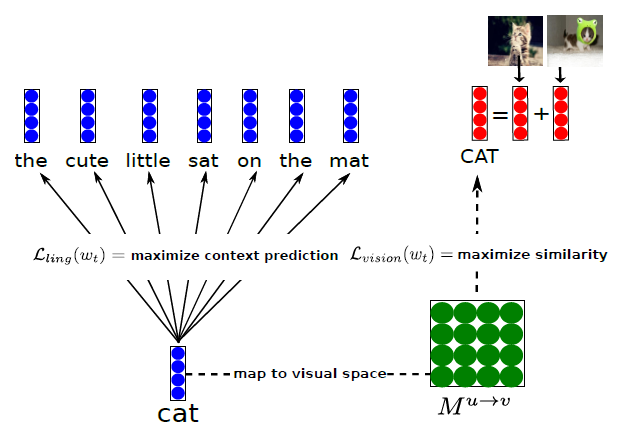
\includegraphics[width=0.8\linewidth]{figures/02-03-img-support-text/img-lazaridou2015combining01} 

}

\caption{From @lazaridou2015combining. The linguistic embedding of the word 'cat' is mapped to a visual space, such that the similarity of vector representations of words and associated images is maximized.}\label{fig:img-lazaridou2015-01}
\end{figure}

Similar instances of a cross-modal mapping can be found for example in \citet{kottur2016visual} (a multimodal extension of the CBOW model specification of word2vec) and in \citet{collell2017imagined}, where visual features are obtained from the forward pass of a CNN, pre-trained on ImageNet (\citet{deng2009imagenet}) and a mapping function from the textual space to the visual space is obtained as a result of the training process. Also in this case it is possible to generate a visual representation from the embedding of a certain word, not necessarily present in the training set. In particular, they propose two specifications of the mapping function: a simple linear mapping and neural network with a single hidden layer. Last but not least, \citet{hill2014learning} recognize that concrete nouns are more likely to have a visual representation. For this reason, they map a set of concrete words (CSLB, \citet{devereux2014centre}) to ``bags of perceptual/visual features'' and every time one of these words is encountered during training, the Skip-gram model they are using stops training on that sentence and instead continues the training on a newly created ``pseudo-sentence'', which takes into consideration the aforementioned bag of perceptual features. This list is unfortunately not exhaustive and there are other models with similar ideas, for example \citet{ailem2018probabilistic} or \citet{kiros2018illustrative}.

The aforementioned papers and related models focus on the modeling of semantics of words. Nonetheless, there are models designed to address tasks at sentence-level, such as sentiment analysis or sentence entailment. \citet{kiela2017learning} employ a bidirectional Long Short-Term Memory (LSTM, \citet{hochreiter1997long}) architecture to model sentence representations, in order to gain information from the text in both directions. The goal is again to encode a sentence and ground it in an image. Textual embeddings are obtained with GloVe (\citet{pennington2014glove}) and they are then projected on a grounded space with a linear mapping. This grounded word vector serves as input for the bidirectional LSTM, which is trained together with the linear mapping. Their model is versatile and depending on the loss function specification, it can not only propose alternative captions to an image (which is a way to frame sentence equivalence tasks) but also predict captions from images or perform both tasks at the same time. This last point highlights an important characteristic of many of the models discussed in this subchapter: even though the focus is on the empowerment of pure language models with the addition of visual elements, some of the models discussed here can be used for purposes other than pure language tasks. The control over which task is performed is usually exercised by either specifying different loss functions (as in the last model described) or setting properly certain hyperparameters (such as in the previously described model by \citet{silberer2014learning}).

\hypertarget{the-transformers-era}{%
\subsection{The Transformers Era}\label{the-transformers-era}}

A turning point for the field of NLP was \citet{vaswani2017attention}'s paper ``Attention is all you need'', where the authors proposed for two machine translation tasks a novel architecture, the Transformer (not to be confused with the giant robots from the Michael Bay's blockbuster movies!), which leverages only the attention mechanism. Even though an exhaustive description of the Transformer architecture is beyond the scope of this subchapter, it is worth mentioning why they became so popular over the past four years in the field of NLP (among others), in comparison to Recurrent Neural Networks (RNNs) and Long Short-Term Memory networks (LSTMs).

Well, the three main properties of Transformers are the following:

\begin{itemize}
\tightlist
\item
  Self-Attention
\item
  Parallel input processing
\item
  Positional embeddings\footnote{It may be argued that this point is a necessity to be able to work on sequences rather than a strength.}
\end{itemize}

When feeding for example a textual sentence to a RNN, the network deals with one word after the other in a sequential fashion and one of the known issues is the fact that information contained in earlier parts of the sequence tend to ``fade away'' as the sentence is analyzed further: newer inputs carry a larger influence on the outputs at a given step. LSTMs try to mitigate this problem by introducing a component called ``gate'', which regulates the information flow, namely which information from the past inputs need to be ``remembered'' by the model. The goal is to capture long-term dependencies among different parts of the sentence fed into the model.\\
On the contrary, thanks to the Self-Attention mechanism, at each step Transformers can access previous steps, thus limiting to a minimum the loss of information. Moreover, inputs are processed not sequentially but all at the same time, thus allowing to capture dependencies by looking at the sentence \emph{as a whole} and this could make a fundamental difference in many downstream applications: for example in the German language, in dependent clauses (``Nebensaetze''), the verb comes at the end of the phrase but it determines the verbal case of the nouns that come \emph{before} the verb. Thus Transformer could potentially capture the dependencies between the verb coming at the end of the sentence and the words at the beginning. Lastly, Transformers encode for every input information on its position within a sentence, since it is often the case, that the importance and meaning of a certain word varies depending on its position within a sentence. These were the Transformers, in a nutshell.

But Transformers did not only bring a change of paradigm in terms of architectures. First, while for models in the pre-Transformers era described before, the focus was on the ability of word embeddings to capture similarity among words, now the focus has shifted more on downstream tasks (more on this later in the evaluation section), encompassing not only pure linguistic ones but also tasks with visual components, such as for example, visual question answering. It is now more difficult (but not impossible) to draw a line between models where ``images support pure language models'' (the object of this subchapter) and models which could be actually categorized as ``vision and language'' models but they can be employed also to solve pure linguistic tasks. This issue brings another peculiarity of many Transformers-base models, namely their ``universal vocation'': without loss of generality we could say that the idea is now to design powerful (multimodal) pre-training (mostly \emph{self-supervised}) tasks capable of generating task-agnostic representations, whose encoded knowledge can be efficaciously transferred to diverse downstream tasks, limiting the amount of labeled data necessary to fine-tune the models (this is the so-called \emph{few-shot learning}).

Let's briefly discuss two examples, Flava (\citet{singh2022flava}) and UniT (\citet{hu2021unit}). Flava has two separate encoders for images and text and a multimodal encoder, all based on the Vision Transformer (\citet{dosovitskiy2020image}). Unimodal pre-training consists of masked image modeling (where a set of image patches are to be reconstructed from other unmasked image patches) and masked language modeling. Multimodal pre-training tasks consist instead of a global contrastive loss (maximization of cosine similarities between paired images and text), a masked multimodal modeling (where image patches and text tokens are masked) and an image-text matching task. The model is pre-trained jointly on unimodal and multimodal datasets and then evaluated (fine-tuned) on 22 vision tasks, 8 pure linguistic tasks and 5 vision and language tasks.\\
UniT has an image encoder and a text encoder, a multimodal domain-agnostic decoder and task-specific heads. There is no pre-training on multimodal data and the model is trained end-to-end on 7 tasks (vision, language and vision an language) and 8 datasets, with the idea that solving different tasks across domains in a jointly fashion should prevent general knowledge from being lost due to fine-tuning over particular downstream tasks.

These two examples clearly show what it is meant by ``universal vocation'' of many modern Transformer-based models. But there are still models specifically designed to solve pure language tasks and in the following pages, two of them will be described.

\hypertarget{vokenization}{%
\subsubsection{Vokenization}\label{vokenization}}

It is often difficult for a child to describe the meaning of a certain word. A child might not be able to describe what a lion is but if he is given pictures of different animals he might be very well able to point at the picture of a lion. \emph{Visual pointing} could thus act as a form of supervision to natural language. Is it possible to build within a pure language model a form of visual supervision, which mimics the visual pointing often adopted by children? This is exactly the problem that \citet{tan2020vokenization} try to address: how to associate to each textual representation (token) a visual representation (Voken).

Let's suppose we had a dataset of word(token)-image pairs. We could integrate in the pre-training framework of pure language models the following \emph{Voken-Classification} task:

\[\mathcal{L}_{VOKEN-CLS}(s)=-\sum_{i=1}^{l}log\ p_{i}(v(w_{i};s)|s) \]
\[\textbf{h}_{1}, \textbf{h}_{2},...,\textbf{h}_{l}=languagemodel(w_{1},w_{2},...,w_{l}) \]
\[p_{i}(v|s)=softmax_{v}\{W\textbf{h}_{i}+b\}\]
where \(\{h_i\}\) is the feature representation of each token in a sentence \(s=\{w_i\}\) extracted from a language model (such as BERT) and the vokens originate from a \textbf{finite} set of images \(X\). Each \(h_i\) is then transformed into a probability distribution through a softmax layer, with the voken-classification loss defined as the negative log-likelihood of all related vokens.\\
The model architecture would then be:

\begin{figure}

{\centering 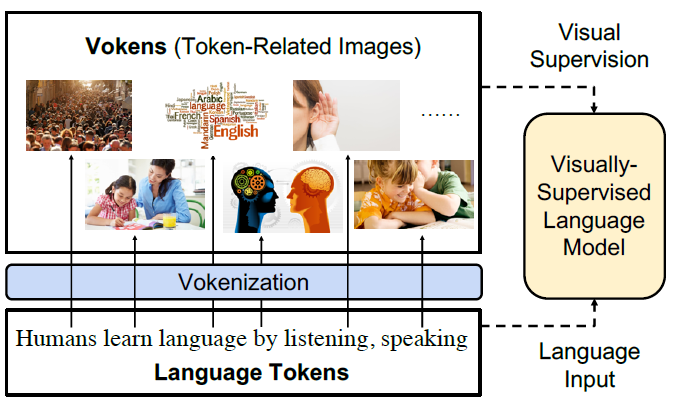
\includegraphics[width=0.7\linewidth]{figures/02-03-img-support-text/img-tan2020-04} 

}

\caption{From @tan2020vokenization. Visually supervised the language model with token-related images, called Vokens.}\label{fig:img-tan2020-04}
\end{figure}

Everything sounds fantastic! There is only one small pitfall: a set of \(X\) of images for all tokens does not exist! Could we find a proxy for such a set? One might consider image-captioning datasets such as MS COCO (\citet{lin2014microsoft}). But also this suboptimal solution is problematic.

\begin{figure}

{\centering 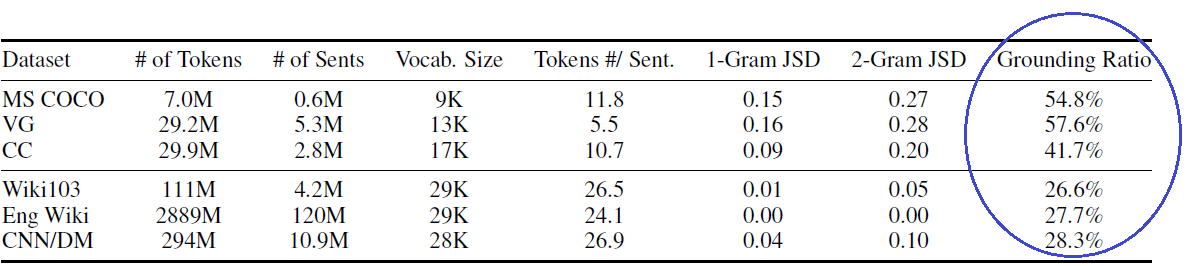
\includegraphics[width=1\linewidth]{figures/02-03-img-support-text/img-tan2020-01} 

}

\caption{From @tan2020vokenization. Statistics of image-captioning dataset and other natural language corpora. VG, CC, Eng Wiki, and CNN/DM denote Visual Genome, Conceptual Captions, English Wikipedia, and CNN/Daily Mail, respectively. JSD represents Jensen–Shannon divergence to the English Wikipedia corpus.}\label{fig:img-tan2020-01}
\end{figure}

The \emph{Grounding Ratio} is defined as the proportion of tokens in a dataset which are related to a specific visual representation (i.e.~the tokens are \emph{visually grounded}), such as ``dog'', ``table'' and the like. In figure \ref{fig:img-tan2020-01} it is striking that only around one third of tokens contained in pure language corpora such Wiki103, English Wikipedia and CNN/DM are visually grounded in image captioning datasets\footnote{From an operative point of view, the authors consider a token type ``visually grounded'' if it has more than 100 occurrences in MS COCO}. It is not possible to rely (only) on image captioning datasets to build the Voken-Classification task. But the fact that a word/token does not have a visual representation in one of these datasets, it does not mean that it is not possible to visually represent the word/token. Would it be possible to associate images to words/tokens not directly visually grounded? Well, the answer is yes!

\begin{figure}

{\centering 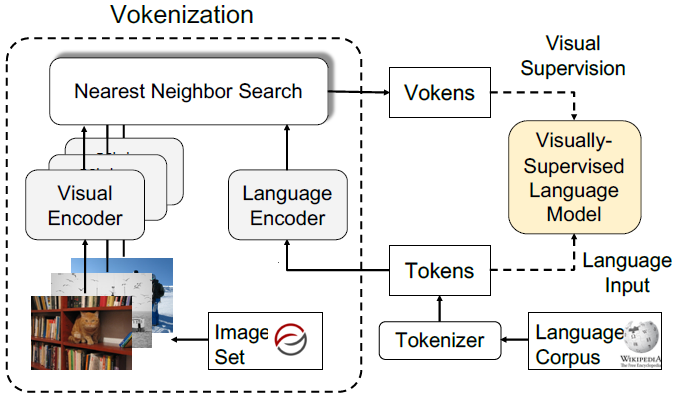
\includegraphics[width=0.8\linewidth]{figures/02-03-img-support-text/img-tan2020-05} 

}

\caption{From @tan2020vokenization. The Vokenization process. A contextualized image (visual token, Voken) is retrieved for every token in a sentence and with this visual token, visual supervision is performed.}\label{fig:img-tan2020-05}
\end{figure}

The \textbf{Vokenization} is a process to \emph{assign} every token \(w_i\) contained in a sentence \(s\) to a visual representation (called \emph{voken}) originating not from a generative model but rather from a finite set of images \(X=\{x_1,...,x_n\}\). The voken \(v(w_i;s)\) is the image from \(X\) which maximizes the following \emph{Relevance Score Function}:
\[v(w_i;s)=arg\ max_{x\in X}r_{\theta^{*}}(w_i,x,s)\]
This function takes into account not only the token \(w_i\) itself, but also the context (the sentence) and it is parametrized by \(\theta\) with \(\theta^{*}\) being the optimal value (which has to be estimated).

\hypertarget{the-relevance-score-function-model-training-inference}{%
\paragraph{The Relevance Score Function: Model, Training, Inference}\label{the-relevance-score-function-model-training-inference}}

The Relevance Score Function is defined as the inner product of the language feature representation \(f_{\theta}(w_i,s)\) and the visual feature representation \(g_{\theta}(x)\):
\[f_{\theta}(w_i,s)^Tg_{\theta}(x)\]
Supposing \(h_1,...,h_l\) and \(e\) are the embeddings originating from pre-trained language and visual encoders respectively (in the paper the authors use BERT and ResNeXt), the language and visual representations are obtained first by applying multi-layer perceptrons \(w\_mlp_{\theta}\) and \(x\_mlp_{\theta}\) to downproject the embeddings from the pre-trained models to a common vector space and secondly they are normalized (with L2-Norm):

\[ \textbf{f}_{\theta}(w_{i};s)= \frac{w{\_}mlp_{\theta}(\textbf{h}_{i})}{||w{\_}mlp_{\theta}(\textbf{h}_{i})||} \]
\[ \textbf{g}_{\theta}(x)= \frac{x{\_}mlp_{\theta}(\textbf{e})}{||x{\_}mlp_{\theta}(\textbf{e})||} \]
With respect to the training of the model, to estimate the optimal value for the parameter \(\theta\), image-captioning datasets, which are collections of sentence-image pairs, are employed. Operationally, for every sentence \(s_k\) associated to image \(x_k\) in the image-captioning dataset, each token \(w_i\) in \(s\) is associated to \(x_k\) and the \emph{hinge loss} is used to estimate the optimal value of \(\theta^*\):

\[ \mathcal{L}_{\theta}(s,x,x')=\sum_{i=1}^{l}max(0,M-r_{\theta}(w_{i},x,s)+r_{\theta}(w_{i},x',s))\]

The goal is to maximize the Relevance Score Function between aligned token-image pairs \((w_i,x;s)\) and to minimize the score for unaligned pairs \((w_i,x^{'};s)\) by at least a margin \(M\), with \(x^{'}\) being a randomly sampled image from the image captioning dataset \textbf{not} associated to sentence \(s\).

Once we have the language feature representation \(f_{\theta}(w_i,s)\) for each token in our language corpus and the optimal estimate of \(\theta\), how is it possible to find the image \(x\) encoded with the visual feature representation \(g_{\theta}(x)\), which maximizes the Relevance Score Function? As said earlier, the function is expressed as the inner product of the textual and visual representations and since the feature vectors have euclidean norm equal to 1, the inner product maximization problem is equivalent to a nearest neighbor search problem. It is just sufficient to find the vector \(g_{\theta}(x)\) which is the nearest neighbor of \(f_{\theta}(w_i,s)\)\footnote{The proof is straightforward. Let \(X\in \mathbb{R}^l\) and have euclidean norm equal to 1, which means \(||X||_{2}=1\). In the nearest neighbor search we need to find the vector \(Y\in \mathbb{R}^l\), also with norm equal to 1, which has minimal euclidean distance with \(X\). This is the quantity to be minimized:
  \begin{align*}
  d(X,Y) &=\sqrt{\sum_{i=1}^{l}{(x_i-y_i)^2}}
    \\&\stackrel{squared}{=} \sum_{i=1}^{l}{x_i^2}+\sum_{i=1}^{l}{y_i^2}-2\sum_{i=1}^{l}{x_iy_i}
    \\&\stackrel{}{=}||X||_{2}^2+||Y||_2^2-2X^TY
    \\&\stackrel{Norm-1}{=}1+1-2X^TY
    \\&\stackrel{}{=}2(1-X^TY)
  \end{align*}
  And through these simple algebraic manipulations, it is possible to see that minimizing the euclidean distance between \(X\) and \(Y\) is equivalent to maximize \(X^TY\), which is the inner product. This proves the equivalence between inner product maximization and nearest neighbor search.}.

With this process, it is thus possible to assign a visual representation, a voken, to any word/token in a language corpus, pooling from a finite set of images. The problem of the low Grounding Ratio outlined above is solved and the Voken-Classification task could be integrated in the pre-training framework of any pure language model. Moreover, the authors propose a method called \emph{Revokenization}, which allows to transfer vokens generated using a particular tokenizer to frameworks which employ other tokenizers.

\hypertarget{one-step-further-the-power-of-imagination}{%
\subsubsection{One Step Further: The Power Of Imagination}\label{one-step-further-the-power-of-imagination}}

Wikipedia defines \emph{imagination} as ``the production or simulation of novel objects, sensations, and ideas in the mind without any immediate input of the senses''. Indeed, humans do not only associate words with real images, but also leverage the ability to \emph{imagine} words/concepts: imagination can help the human brain solve problems with limited supervision or sample points by empowering its generalization capabilities. Until now we discussed language models supported by visual information in form of \emph{real} images (e.g.~those retrieved from image-captioning datasets). But with the recent advancements in the field of generative models for images, it is for sure worth investigating if these generative models can help pure language models to produce better representations of words. In particular, the framework proposed by \citet{lu2022imagination}, \textbf{iACE (Imagination-Augmented Cross-Modal Encoder)} will now be discussed: the idea is simply to use a generative model to obtain a visual representation of a textual input and then use these imagined representations as ``imagination supervision'' to pure language models.

\begin{figure}

{\centering 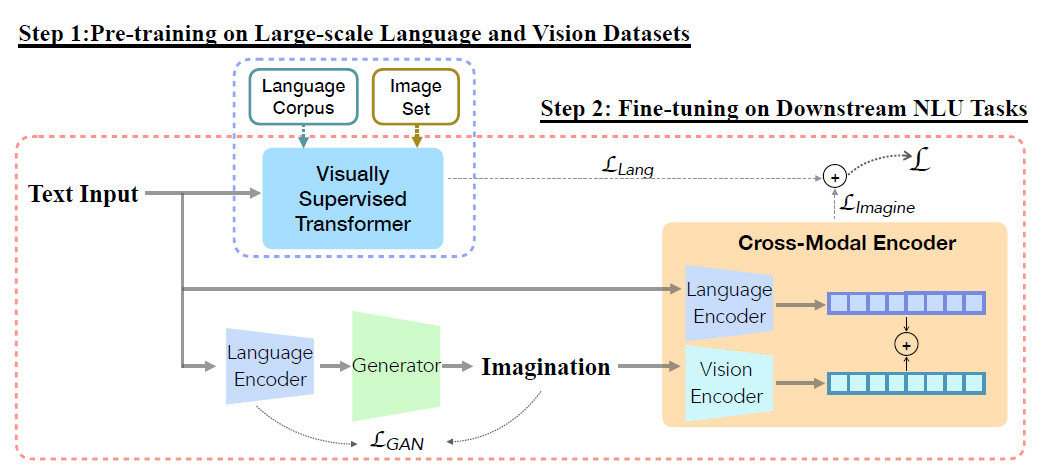
\includegraphics[width=1\linewidth]{figures/02-03-img-support-text/img-lu2022-01} 

}

\caption{From @lu2022imagination. The generator $G$ visualize imaginations close to the encoded texts by minimizing $\mathcal{L}_{GAN}$. The cross-modal encoder $E_c$ learns imagination-augmented language representation. Two-step learning procedure consists of: 1) pre-train a Transformer with visual supervision from large-scale language corpus and image set, 2) fine-tune the visually supervised pre-trained Transformer and the imagination-augmented cross-modal encoder on downstream tasks.}\label{fig:img-lu2022-01}
\end{figure}

This framework has two main components:

\begin{itemize}
\tightlist
\item
  the \textbf{imagination generator \(G\)}: given an input text \(x\), VQGAN (\citet{esser2021taming}) is used to render an ``imagination'' \(i\) of \(x\) and CLIP (\citet{radford2021learning}) is used to see how well the generated image \(i\) is aligned to the input text \(x\). This generative framework is known as VQGAN+CLIP
\item
  \textbf{Cross-modal Encoder \(E_c\)}: the input text and the rendered imagination are firstly encoded with a language and a visual encoder respectively and then CLIP is employed as cross-modal encoder with inputs being text-imagination pairs
\end{itemize}

The learning procedure is composed of two main steps (depicted in figure \ref{fig:img-lu2022-01}): the first step consists in the pre-training of a visually supervised Transformer. In particular, the Voken-Classification task described before is employed, alongside a masked language modeling task. This is the baseline model, where no information from the ``imagination'' procedure comes yet into play. The second step is the \emph{imagination-augmented fine-tuning} with two downstream datasets \(D\) (GLUE, \citet{wang2018glue} and SWAG, \citet{zellers2018swag}).\\
On one side, the visually-supervised Transformer (the baseline) relies only on the textual input during the fine-tuning phase and the following loss function is employed:

\[ \mathcal{L}_{Lang}=-\sum_{j=1}^{|D|}\sum_{k=1}^{K}y_{k}\ log\ p_{k}(d_{j}(t)|D) \]

On the other hand, the \emph{iACE} is trained to minimize the following cross-entropy loss:

\[ \mathcal{L}_{Imagine}=-\sum_{j=1}^{|D|}\sum_{k=1}^{K}y_{k}\ log\ p_{k}(d_{j}(t,v)|D) \]

with \(t\) and \(v\) being the textual and imagined features representations respectively, \(j\) indicates the \(j\)-th data sample in dataset belonging to dataset \(D\), \(K\) is the number of classes and \(p_k\) is the conditional distribution of \(d_j\).
Training takes place in a jointly fashion and both losses, the imagination-augmented one \(\mathcal{L}_{Imagine}\) and the pure language loss \(\mathcal{L}_{Lang}\) are linearly combined, with \(\lambda\) being a balance factor:

\[\mathcal{L}=\lambda\mathcal{L}_{Imagine}+(1-\lambda)\mathcal{L}_{Lang} \]

To sum up, this model-agnostic framework uses \emph{generated images} for visual supervision and could be integrated on top of pure language models (such as BERT) or visually supervised models (such as the Voken model, which uses Vokens, real images for visual supervision).

\hypertarget{was-it-worth}{%
\subsection{Was It Worth?}\label{was-it-worth}}

In this subchapter we investigated how visual inputs can support pure language models in capturing the semantics of words. We started with simple concatenation of linguistic and visual features and ended up with Transformer-based models, which are able to shape different word embeddings for the same word by taking into account also the context (the sentence). But now the question arises: with the addition of visual information, do we obtain word embeddings that are better than those from pure language models? In other words, is what we all have so far discussed worth? Well, as it is often the case in scientific research, the answer is: ``it depends!''

Individual evaluation of each single model might not be ideal because each model has its peculiarities and it is impractical to make a direct comparison among them. It is more useful to capture and discuss the themes which are common to many models, in order to understand their strengths and weaknesses. This is how we will proceed and we will also differentiate between evaluation before Transformers and evaluation after Transformers.

\hypertarget{evaluation-in-the-pre-transformers-era}{%
\subsubsection{Evaluation In The Pre-Transformers Era}\label{evaluation-in-the-pre-transformers-era}}

Before the advent of Transformers, the evaluation focus was on the degree of alignment between learned semantic representations (word embeddings) and representations by human speakers, in form of correlation between model-based and human-based word-similarity judgments. Three main types of similarity are usually considered:

\begin{itemize}
\item
  Semantic similarity, e.g.~``pasta is similar to rice''
\item
  Semantic relatedness, e.g.~``Bear is related to mountain''
\item
  Visual similarity, e.g.~``cucumbers look like zucchinis''
\end{itemize}

The evaluation pipeline could be summarized as follows:

\begin{figure}

{\centering 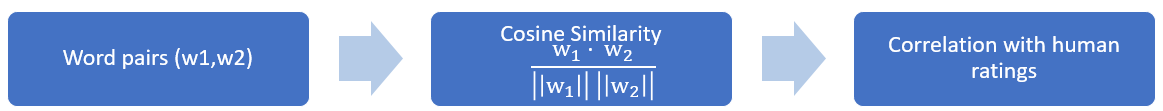
\includegraphics[width=1\linewidth]{figures/02-03-img-support-text/img-eval01} 

}

\caption{Pipeline for intrisinsic evaluation of semantic representations. In the first step, the cosine similarity between two word embeddings w1 and w2 is used as similariry measure and in a second step, the correlation with human speakers'assessment is computed to gauge the quality of the embeddings. The higher the correlation, the better the embeddings.}\label{fig:img-eval01}
\end{figure}

Word embeddings are vectors and to measure the degree of similarity between two vectors, the \emph{Cosine Similarity} is often used in the literature. In an ideal setting, we would have word embeddings with the following characteristics: if two words are semantically similar, the two embedding vectors should be similar and their cosine similarity should go towards 1. If the two words are unrelated, the embedding vectors should be orthogonal to each other and as a consequence, the cosine similarity should go towards zero. Lastly, if two words are negatively related, the two embedding vectors should point at opposite directions and the cosine similarity should go towards -1.
Once these similarity measures between word pairs are computed, in order to measure the quality of the embeddings several benchmarks can be employed, such as MEN (\citet{bruni2014multimodal}), WordSim353 (\citet{agirre2009study}) and SimLex999 (\citet{hill2015simlex}). These datasets could be described as collections of word pairs and associated similarity ratings by human speakers. Operationally, this means that real people were asked if a pair of words was related or not and to which degree, on a scale between -1 (negatively related) to +1 (semantically equivalent). The higher the correlation between the cosine similarity and the similarity judgments by humans, the higher the quality of the word embeddings. Having done this methodological premise, let's discuss the performance of these pre-Transformer models!

Since the goal of these models is to enhance pure language models with the addition of visual inputs, the baseline in the evaluation is always one (or more) pure language model(s). Well, do visually grounded embeddings outperform non-grounded ones? What emerges from virtually all papers is that visual grounding can actually help get a better semantic representation of \emph{concrete} concepts, such as ``cat'', ``table'', ``bicycle'', whereas they do not help much with the representation of abstract concepts such as ``love'' and ``peace''.

\begin{figure}

{\centering 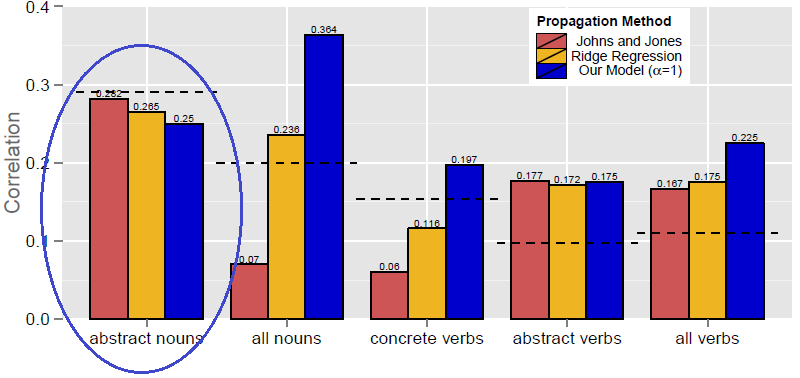
\includegraphics[width=1\linewidth]{figures/02-03-img-support-text/img-2014hill-01} 

}

\caption{From @hill2014learning: Each bar represents a different model settings and the dashed line indicates the pure linguistic benchmark model.}\label{fig:img-2014hill-01}
\end{figure}

In figure \ref{fig:img-2014hill-01} we can see that pure language models still perform better than models with visual inputs when it comes to the representation of abstract \emph{nouns}. Another example is \citet{kiela2017learning}: they found that their models perform better when tested on datasets with a higher degree of concreteness and the same conclusion is reached by \citet{collell2017imagined}, which state that visual information can empower the representations of concepts that are to a certain extent visual. To sum up, effective semantic representation of abstract concepts constitute the main limitation common to many of the models discussed in this section.

\hypertarget{evaluation-in-the-post-transformers-era}{%
\subsubsection{Evaluation In The Post-Transformers Era}\label{evaluation-in-the-post-transformers-era}}

A limitation of the \emph{intrinsic} evaluation metrics is the high degree of subjectivity: the \emph{similarity} between two concepts depends in many instances on the experience, cultural background and preferences of the human observers. This is why the evaluation focus has now shifted to a more \emph{extrinsic} dimension: how well do the models perform in downstream tasks? The problem of the ``lack of objectivity'' is thus solved because on downstream tasks there is no room for opinions. The datasets used to train the models are also different and the most widely used are:

\begin{itemize}
\tightlist
\item
  GLUE (\citet{wang2018glue}): 9 tasks, including single-sentence tasks (e.g.~sentiment analysis), similarity tasks (e.g.~paraphrasing), inference tasks (e.g.~textual entailment)
\item
  SQuAD (\citet{rajpurkar2016squad}): question/answer pairs
\item
  SWAG (\citet{zellers2018swag}): multiple choice questions about grounded situations
\end{itemize}

As previously discussed, many Transformer-based models have universal vocation: they are built to solve a heterogeneous range of tasks from the language and vision domain. If we thus consider only performance on pure language tasks, the following two tables from \citet{tan2020vokenization} are insightful:

\begin{figure}

{\centering 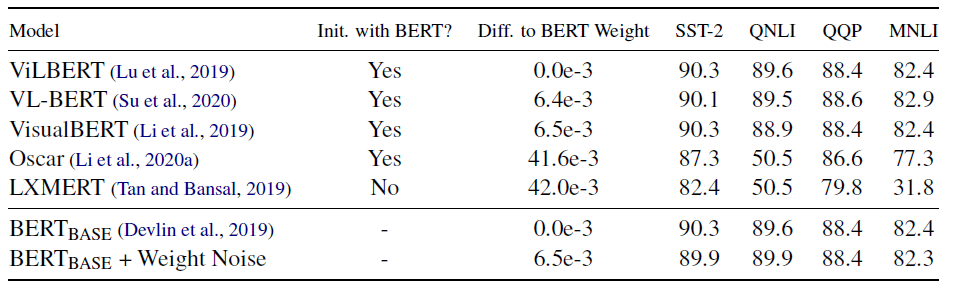
\includegraphics[width=1\linewidth]{figures/02-03-img-support-text/img-tan2020-02} 

}

\caption{From @tan2020vokenization. Results of vision-and-language pre-trained models (universal models) on GLUE tasks compared to baseline models (BERT).}\label{fig:img-tan2020-02}
\end{figure}

\begin{figure}

{\centering 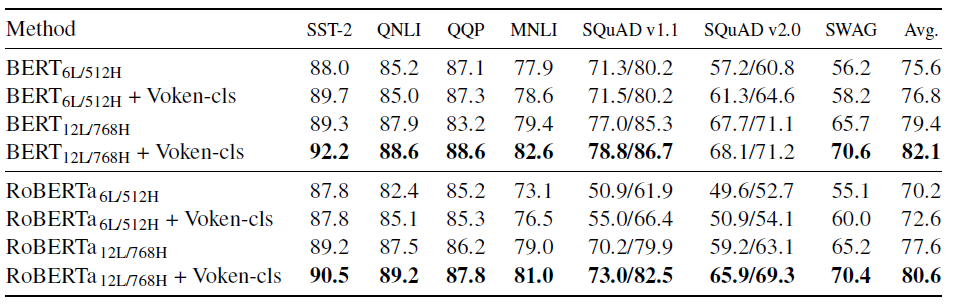
\includegraphics[width=1\linewidth]{figures/02-03-img-support-text/img-tan2020-03} 

}

\caption{From @tan2020vokenization. Fine-tuning results of different pre-trained models w/ or w/o the voken classification task (denoted as“Voken-cls”).}\label{fig:img-tan2020-03}
\end{figure}

It is straightforward: unlike in the pre-Transformers Era, where grounded word embeddings could improve performance over baselines, Transformer-based universal models \textbf{do not} outperform pure language models such as BERT or RoBERTa. Nonetheless, the addition of visual supervision (the Voken-Classification task) in the pre-training framework can boost performance above the level of pure language models.

\citet{pezzelle2021word} analyzed the \emph{intrinsic} quality of embeddings of some vision and language (``universal'') models:

\begin{figure}

{\centering 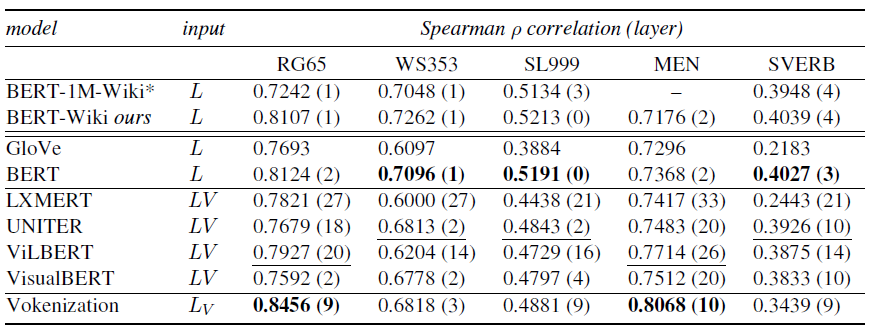
\includegraphics[width=1\linewidth]{figures/02-03-img-support-text/img-pezzele2021-01} 

}

\caption{From @pezzelle2021word. Spearman’s rank correlation between similarities computed with representations by all tested models and human similarity judgments in the five evaluation benchmarks.}\label{fig:img-pezzele2021-01}
\end{figure}

\begin{figure}

{\centering 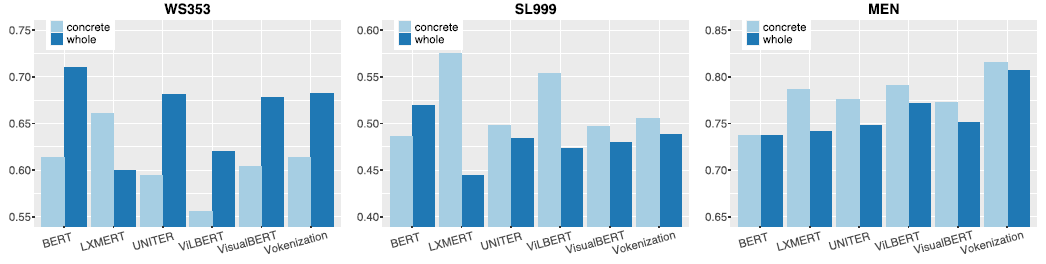
\includegraphics[width=1\linewidth]{figures/02-03-img-support-text/img-pezzele2021-02} 

}

\caption{From @pezzelle2021word. Correlation between model and human similarity ratings on WordSim353, SimLex999 and MEN. Each barplot reports results on both the whole benchmark and the most concrete subset of it.}\label{fig:img-pezzele2021-02}
\end{figure}

From this \emph{intrinsic} evaluation perspective (which was popular in the pre-Transformers Era), vision and language models do not generally outperform domain-specific models such as BERT and also in this case the only real competitor of pure language models is a model with visual supervision (again, Vokenization).

The bar plots depict correlation between human- and model-based similarity ratings, differentiating between the most \emph{concrete} concepts contained in a certain dataset\footnote{See \citet{brysbaert2014concreteness} for information on how \emph{concreteness} of a word can be estimated.} and the whole dataset (thus including more abstract concepts). The results confirm the trend: multimodal models are more effective than pure language models at representing concrete words but in many instances they still lag behind when it comes to more abstract concepts.

Last but not least, few words need to be spent on a topic which has been steadily gaining relevance: \textbf{Few-Shot Learning}. To train and test models, a large pool of paired images and texts is often needed and the creation of many of the datasets used in fine-tuning required a huge data collection effort, which had to be performed by human agents. This implies that the creation of such data pools can be very costly. For this reason, there is a growing interest in creating models able to cope with low-resource settings. This boils down to the question: can a model perform well on downstream tasks even with just a \emph{limited number} of training examples? The goal is actually once again, to mimic how humans learn: a person does not need to see one thousand pictures of a table, to be able to recognize a table\ldots{}

\begin{figure}

{\centering 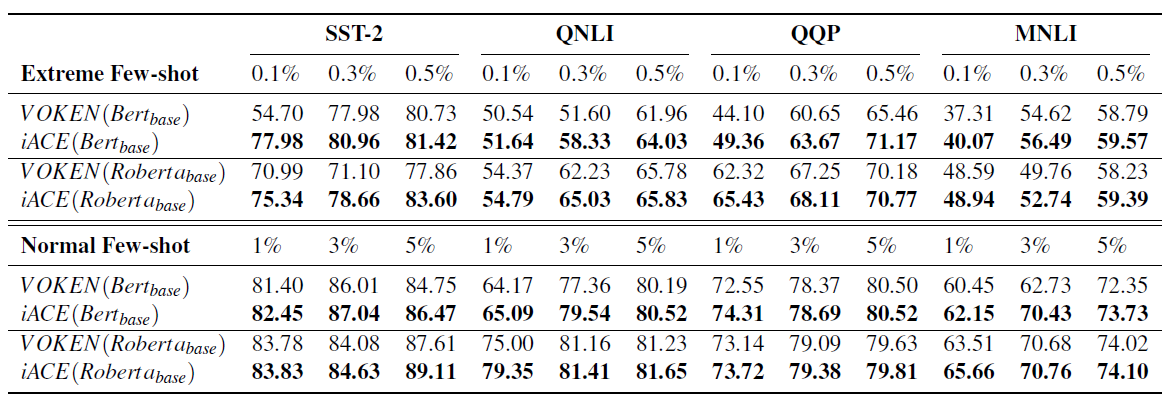
\includegraphics[width=1\linewidth]{figures/02-03-img-support-text/img-lu2022-02} 

}

\caption{From @lu2022imagination. Model-agnostic improvement in Few-shot Setting with GLUE benchmark.}\label{fig:img-lu2022-02}
\end{figure}

This table from \citet{lu2022imagination}, where models are trained using only up to 5\% of the training set, shows for example the ability for a model supervised with ``imagination'' (which was a generated visual representation of a certain textual input) to outperform models with only simple visual supervision (the Voken-model). This is just an example, but the ability to perform well in \emph{few-shot} settings has become the touchstone of the evaluation modern multimodal models.

\hypertarget{the-end-of-this-story}{%
\subsection{The End Of This Story}\label{the-end-of-this-story}}

We started this story with the \emph{Symbol Grounding Problem}, which affirms that to grasp the meaning of a word, the word has to be put in a context other than the pure linguistic one. We thus investigated some of the architectures proposed to ground words in a visual space in form of static images. The goal (hope) is to better capture the semantics of words, in form of better word embeddings, to be employed in heterogeneous tasks, from \emph{semantic-similarity} to downstream tasks, such as \emph{sentiment analysis}.\\
From this brief analysis it emerges that grounding words in images can actually improve the representation of \emph{concrete} concepts, whereas visual grounding does not seem to add value to pure language models when it comes to \emph{abstract} concepts. Nonetheless, forms of visual supervision like the \emph{Voken-Classification} task or the employment of generative models which allow to \emph{imagine} words, such as in the \emph{iACE-Framework}, might be the right way to bridge this gap.\\
The Transformers have been a revolution in the field of NLP and with their advent, the trend has now become to build models with pre-training tasks capable of generating powerful task-agnostic word representations. The knowledge gained with these tasks can be then transferred to downstream tasks with the goal to limit the amount of labeled data necessary to fine-tune models. Labeling data is indeed costly: this is why the ability of a model to generalize well when exposed to just few training examples has been steadily gaining importance as evaluation metric. This was the so called \emph{few-shot learning}. Moreover, Transformer-based models have ``universal vocation'': they tend to be multimodal and multi-task, encompassing vision, language and vision and language tasks. This idea might be appealing because humans learn by being exposed to a multitude of different inputs and tasks. But as we have seen, pure language models such as BERT tend to still outperform multimodal multi-task models. There is definitely room for improvement.\\
One might wonder whether the grounding of words in images is the right way to seek a better representation of words. Well, humans learn using all five senses and maybe the answer might be to incorporate in the models more heterogeneous perceptual information: not only static images but also videos, speech and the like. The debate is still open: the story \emph{goes on}\ldots{}

Last but not least, a mention needs to be made on concrete applications of these image-empowered word-embeddings. The use of images to support linguistic models has been experimented in several fields, from \emph{Dialogue Response Generation} (e.g.~\citet{sun2021multimodal}) to \emph{Machine Translation}, where for example \citet{ive2019distilling} found images to improve the quality of translation when the textual context is generic and/or ambiguous. The number of potential applications of the models described in this subchapter is growing steadily in the scientific community. But this is yet \emph{another} story\ldots{}

\hypertarget{appendix-selected-models---summary}{%
\subsection{Appendix: Selected Models - Summary}\label{appendix-selected-models---summary}}

The following table contains a summary of selected language models augmented with visual components. For each model, the following information are reported:

\begin{itemize}
\item
  Pure language model and pretraining data
\item
  Visual features and pretraining data
\item
  Fusion strategy of the two modalities
\item
  Benchmarks/baselines for evaluation:

  \(\color{green}\blacktriangle\) better performance over baseline(s)\\
  \(\color{orange}\bullet\) mixed performance results over baseline(s)\\
  \(\color{red}\blacktriangledown\) worse performance over baseline(s)\\
\end{itemize}

The table is available in a more readable format \href{Table-ch2-3-final.pdf}{here}.

\begin{longtable}[]{@{}llllllllll@{}}
\toprule
\begin{minipage}[b]{0.00\columnwidth}\raggedright
Year\strut
\end{minipage} & \begin{minipage}[b]{0.06\columnwidth}\raggedright
Paper\strut
\end{minipage} & \begin{minipage}[b]{0.04\columnwidth}\raggedright
Language model (LM)\strut
\end{minipage} & \begin{minipage}[b]{0.02\columnwidth}\raggedright
LM-Pre-training sources\strut
\end{minipage} & \begin{minipage}[b]{0.07\columnwidth}\raggedright
Visual elements (IMG)\strut
\end{minipage} & \begin{minipage}[b]{0.05\columnwidth}\raggedright
IMG-Pre-training sources\strut
\end{minipage} & \begin{minipage}[b]{0.25\columnwidth}\raggedright
Multimodal representation and model description\strut
\end{minipage} & \begin{minipage}[b]{0.08\columnwidth}\raggedright
Testset/Fine-tuning\strut
\end{minipage} & \begin{minipage}[b]{0.05\columnwidth}\raggedright
Baseline(s)/model settings/comparison to other models\strut
\end{minipage} & \begin{minipage}[b]{0.13\columnwidth}\raggedright
Results\strut
\end{minipage}\tabularnewline
\midrule
\endhead
\begin{minipage}[t]{0.00\columnwidth}\raggedright
2014\strut
\end{minipage} & \begin{minipage}[t]{0.06\columnwidth}\raggedright
Bruni, Elia, Nam-Khanh Tran, and Marco Baroni. ``Multimodal distributional semantics.''~Journal of artificial intelligence research~49 (2014): 1-47.\strut
\end{minipage} & \begin{minipage}[t]{0.04\columnwidth}\raggedright
Distributional model expressed as a matrix with rows as ``semantic vectors'' representing the meaning of a set of target words. The model is based on co-occurrence counts of words (as a result, the matrix is a squared one).\strut
\end{minipage} & \begin{minipage}[t]{0.02\columnwidth}\raggedright
- ukWaC, 1.9B tokens- Wackypedia, 820M tokens.\strut
\end{minipage} & \begin{minipage}[t]{0.07\columnwidth}\raggedright
(i) Local descriptors to extract low-level visual features(ii) Assign local descriptors to cluster of visual words (bag of words) to build the vector representation of an image(iii) Sum up visual words co-occurrence to across all images/instances to get co-occurrence counts related to a target word (the resulting matrix is a squared one).\strut
\end{minipage} & \begin{minipage}[t]{0.05\columnwidth}\raggedright
ESP-Game dataset, 100K images.\strut
\end{minipage} & \begin{minipage}[t]{0.25\columnwidth}\raggedright
Only words for which there is a related image are considered.Two steps to build multimodal representations:(i) Textual and visual matrices are concatenated and projected into a common latent multimodal space with a singular value decomposition. From this matrix, the ``textual mixed matrix'' and the ``visual mixed matrix'' are extracted(ii) Association between words is assessed with cosine similarityTwo fusion methods to estimate similarity of pairs:- Feature level fusion: linear combination of textual and visual mixed matrix and then similarity estimation- Scoring level fusion: word similarity computed on both textual and visual mixed matrices separately and then the final score is a linear combination of the twoIn both methods the weights in the linear combinations are hyperparameter.\strut
\end{minipage} & \begin{minipage}[t]{0.08\columnwidth}\raggedright
- WordSim353- MEN.\strut
\end{minipage} & \begin{minipage}[t]{0.05\columnwidth}\raggedright
- Text mixed embeddings only- Visual mixed embeddings only- Equally weighted versions of feature and scoring level fusion model settings- Several ``fine tuned'' versions of fusion and scoring level fusion model settings.\strut
\end{minipage} & \begin{minipage}[t]{0.13\columnwidth}\raggedright
\(\color{green}\blacktriangle\)Multimodal word representations enhance performance of purely textual or visual embeddings\(\color{orange}\bullet\)No alternative model used as a means of comparison.\strut
\end{minipage}\tabularnewline
\begin{minipage}[t]{0.00\columnwidth}\raggedright
2014\strut
\end{minipage} & \begin{minipage}[t]{0.06\columnwidth}\raggedright
Hill, Felix, and Anna Korhonen. ``Learning abstract concept embeddings from multi-modal data: Since you probably can't see what I mean.''~Proceedings of the 2014 Conference on Empirical Methods in Natural Language Processing (EMNLP). 2014.\strut
\end{minipage} & \begin{minipage}[t]{0.04\columnwidth}\raggedright
Skipgram.\strut
\end{minipage} & \begin{minipage}[t]{0.02\columnwidth}\raggedright
400m word Text8 Corpus.\strut
\end{minipage} & \begin{minipage}[t]{0.07\columnwidth}\raggedright
Mapping of words w to a bag of perceptual features b(w), extracted from external sources and encoded in an associative array P. Generation of pseudo sentences based on these perceptual features to be fed into the language model.\strut
\end{minipage} & \begin{minipage}[t]{0.05\columnwidth}\raggedright
- ESP-Game (100K images)- CSLB Property Norms.\strut
\end{minipage} & \begin{minipage}[t]{0.25\columnwidth}\raggedright
~Extension of the Skipgram injecting perceptual information by generating pseudo-sentences based on a bag-of-visual-words. A hyperparameter \(\alpha\) controls the level of perceptual information relative to linguistic input.\strut
\end{minipage} & \begin{minipage}[t]{0.08\columnwidth}\raggedright
USF Dataset.\strut
\end{minipage} & \begin{minipage}[t]{0.05\columnwidth}\raggedright
- Concatenation of linguistic and perceptual features- Canonical Correlation Analysis applied on vectors of both modalities- SVD of matrix of concatenated multimodal representations.\strut
\end{minipage} & \begin{minipage}[t]{0.13\columnwidth}\raggedright
\(\color{green}\blacktriangle\)Concepts, which can directly be represented in the perceptual modality (e.g.~concrete verbs and nouns)\(\color{green}\blacktriangle\)Propagation of perceptual input from concrete concepts (nouns and verbs) to enhance the representation of abstract verbs, those for which no direct representation in the visual space is available\(\color{red}\blacktriangledown\)Abstract nouns (for which is more difficult to find a concrete visual representation) are still more efficiently learned from language-only models.\strut
\end{minipage}\tabularnewline
\begin{minipage}[t]{0.00\columnwidth}\raggedright
2014\strut
\end{minipage} & \begin{minipage}[t]{0.06\columnwidth}\raggedright
Douwe Kiela and Léon Bottou. 2014. Learning Image Embeddings using Convolutional Neural Networks for Improved Multi-Modal Semantics. In Proceedings of the 2014 Conference on Empirical Methods in Natural Language Processing (EMNLP), pages 36--45, Doha, Qatar. Association for Computational Linguistics.\strut
\end{minipage} & \begin{minipage}[t]{0.04\columnwidth}\raggedright
Skipgram.\strut
\end{minipage} & \begin{minipage}[t]{0.02\columnwidth}\raggedright
- Text8 Corpus (400M words)- British National Corpus (100M words).\strut
\end{minipage} & \begin{minipage}[t]{0.07\columnwidth}\raggedright
Seventh layer of a CNN to extract 6144-d features vectors for images, obtained in two ways:- CNN-Mean (average of all features vectors representing images)- CNN-Max (component-wise maximum of all features vectors)\strut
\end{minipage} & \begin{minipage}[t]{0.05\columnwidth}\raggedright
- ImageNet (12.5M images)- Esp-Game (100K images).\strut
\end{minipage} & \begin{minipage}[t]{0.25\columnwidth}\raggedright
Concatenation of visual and textual embeddings.\strut
\end{minipage} & \begin{minipage}[t]{0.08\columnwidth}\raggedright
- MEN- WordSim353 (it captures not only ``relatedness'' but also ``similarity''.\strut
\end{minipage} & \begin{minipage}[t]{0.05\columnwidth}\raggedright
- Skipgram (text-only baseline)- Embeddings - visual only.\strut
\end{minipage} & \begin{minipage}[t]{0.13\columnwidth}\raggedright
\(\color{green}\blacktriangle\)CNN-Mean better on MEN: averaging might capture relatedness better. CNN-Max better on WordSim353.\strut
\end{minipage}\tabularnewline
\begin{minipage}[t]{0.00\columnwidth}\raggedright
2014\strut
\end{minipage} & \begin{minipage}[t]{0.06\columnwidth}\raggedright
Silberer, Carina, and Mirella Lapata. ``Learning grounded meaning representations with autoencoders.''~Proceedings of the 52nd Annual Meeting of the Association for Computational Linguistics (Volume 1: Long Papers). 2014.\strut
\end{minipage} & \begin{minipage}[t]{0.04\columnwidth}\raggedright
Vectors of textual attributes are extracted.\strut
\end{minipage} & \begin{minipage}[t]{0.02\columnwidth}\raggedright
- McRae et al.'s (2005).\strut
\end{minipage} & \begin{minipage}[t]{0.07\columnwidth}\raggedright
Vectors of visual attributes are extracted.\strut
\end{minipage} & \begin{minipage}[t]{0.05\columnwidth}\raggedright
Same dataset as in Silberer et al.~(2013): taxonomy of 636 visualattributes (e.g., has wings, made of wood) andnearly 700K images from ImageNet (Deng et al.,2009) describing more than 500 of McRae et al.'s(2005) nouns.\strut
\end{minipage} & \begin{minipage}[t]{0.25\columnwidth}\raggedright
Stacked (denoising) autoencoders for each single modality and the outputs are concatenated and fed to a stacked bimodal autoencoder which map the inputs to a joint hidden layer.\strut
\end{minipage} & \begin{minipage}[t]{0.08\columnwidth}\raggedright
With McRae et al.'s (2005), two tasks:- word similarity- word categorization.\strut
\end{minipage} & \begin{minipage}[t]{0.05\columnwidth}\raggedright
- Unimodal autoencoders only- Kernelized Canonical Correlation, Hardoon et al.~(2004)- Bruni et al.~(2014).\strut
\end{minipage} & \begin{minipage}[t]{0.13\columnwidth}\raggedright
\(\color{green}\blacktriangle\)Bimodal models outperform unimodal ones\(\color{red}\blacktriangledown\)Training is on attribute-based inputs. Not widely used in the field.\strut
\end{minipage}\tabularnewline
\begin{minipage}[t]{0.00\columnwidth}\raggedright
2015\strut
\end{minipage} & \begin{minipage}[t]{0.06\columnwidth}\raggedright
Lazaridou, Angeliki, Nghia The Pham, and Marco Baroni. ``Combining language and vision with a multimodal skip-gram model.''~arXiv preprint arXiv:1501.02598~(2015).\strut
\end{minipage} & \begin{minipage}[t]{0.04\columnwidth}\raggedright
Skipgram.\strut
\end{minipage} & \begin{minipage}[t]{0.02\columnwidth}\raggedright
Wikipedia 2009, 800M Tokens.\strut
\end{minipage} & \begin{minipage}[t]{0.07\columnwidth}\raggedright
Visual information for 5100 words with an entry in ImageNet, occur \textgreater500 times in the text corpus and have a~ concreteness score \(\geq\) 0.5; sample 100 images for each word and extract a 4096-d array with a CNN; average the vectors of 100 pictures associated to each word to get visual representation.\strut
\end{minipage} & \begin{minipage}[t]{0.05\columnwidth}\raggedright
ImageNet.\strut
\end{minipage} & \begin{minipage}[t]{0.25\columnwidth}\raggedright
The objective function is a linear composition of the language objective L-ling from the Skipgram and a visual objective L-vision.For the L-vision objective two variants are proposed:- MM Skipgram A (MMSA): aligning vectors of visual and linguistic representations (1:1 correspondence assumed)- MM Skipgram B (MMSB): estimate a cross-modal mapping matrix from linguistic onto visual representations.\strut
\end{minipage} & \begin{minipage}[t]{0.08\columnwidth}\raggedright
- MEN- SemSim- VisSim.\strut
\end{minipage} & \begin{minipage}[t]{0.05\columnwidth}\raggedright
- Kiela and Bottou (2014)- Bruni et al.~(2014)- Silberer \& Lapata (2014)- Skipgram (text-only baseline)- Embeddings - visual only- Concatenation- SVD.\strut
\end{minipage} & \begin{minipage}[t]{0.13\columnwidth}\raggedright
\(\color{green}\blacktriangle\)Both MMSA and MMSB better than simpler models (linguistic/vision only, concatenation SVD)\(\color{orange}\bullet\)MMSA and MMSB competitive in relatedness and visual similarity, despite having often less training data than other models\(\color{orange}\bullet\)Visual grounding less effective with abstract words\strut
\end{minipage}\tabularnewline
\begin{minipage}[t]{0.00\columnwidth}\raggedright
2017\strut
\end{minipage} & \begin{minipage}[t]{0.06\columnwidth}\raggedright
Collell, Guillem, Ted Zhang, and Marie-Francine Moens. ``Imagined visual representations as multimodal embeddings.''~Proceedings of the AAAI Conference on Artificial Intelligence. Vol. 31. No.~1. 2017.\strut
\end{minipage} & \begin{minipage}[t]{0.04\columnwidth}\raggedright
300-d GloVe.\strut
\end{minipage} & \begin{minipage}[t]{0.02\columnwidth}\raggedright
Common Crawl corpus, 840B tokens, 2.2M words.\strut
\end{minipage} & \begin{minipage}[t]{0.07\columnwidth}\raggedright
To extract visual features, the last hidden layer of~ a CNN is taken. For each concept, two different ways to combine the extracted visual features:- Averaging (averaging of al features vectors)- Maxpooling (component-wise maximum).\strut
\end{minipage} & \begin{minipage}[t]{0.05\columnwidth}\raggedright
Imagenet.\strut
\end{minipage} & \begin{minipage}[t]{0.25\columnwidth}\raggedright
Mapping from language to vision. No need of 1:1 correspondence between linguistic and visual inputs. Two different mappings are considered:- Linear (MAP-Clin)- Neural Network (MAP-Cnn).\strut
\end{minipage} & \begin{minipage}[t]{0.08\columnwidth}\raggedright
- MEN- WordSim353- SemSim- Simlex999-SimVerb3500- VisSim.\strut
\end{minipage} & \begin{minipage}[t]{0.05\columnwidth}\raggedright
- Kiela and Bottou (2014)- Lazaridou et al.~(2015)- Silberer \& Lapata (2014)- GloVe (text-only baseline)- Concatenation.\strut
\end{minipage} & \begin{minipage}[t]{0.13\columnwidth}\raggedright
\(\color{green}\blacktriangle\)Outperformance in all instances where words have associated images in the training set\(\color{red}\blacktriangledown\)Performance on the zero-shot learning still inferior in many instances to the textual baselines.\strut
\end{minipage}\tabularnewline
\begin{minipage}[t]{0.00\columnwidth}\raggedright
2018\strut
\end{minipage} & \begin{minipage}[t]{0.06\columnwidth}\raggedright
Kiela, Douwe, et al.~``Learning visually grounded sentence representations.''~arXiv preprint arXiv:1707.06320~(2017).\strut
\end{minipage} & \begin{minipage}[t]{0.04\columnwidth}\raggedright
- GloVe for word embeddings- Bidirectional LSTM for sentence representation.\strut
\end{minipage} & \begin{minipage}[t]{0.02\columnwidth}\raggedright
WebCrawl\strut
\end{minipage} & \begin{minipage}[t]{0.07\columnwidth}\raggedright
Image features obtained from the final layer of a ResNet-101.\strut
\end{minipage} & \begin{minipage}[t]{0.05\columnwidth}\raggedright
MS COCO.\strut
\end{minipage} & \begin{minipage}[t]{0.25\columnwidth}\raggedright
Word embeddings are projected to a ground space with a linear mapping. Linear mapping and Bi-LSTM are trained jointly.Three methods to ground sentences in images, captions or both:- Cap2Img: predict latent features of an image from its caption by mapping the (final) hidden state h(T) of the Bi-LSTM to the latent representation of the image. A ranking loss is to be minimized- Cap2Cap: given the caption pair (x,y) describing the same image, the goal is to maximize the joint probability of y given x. Negative log-likelihood as loss.- Cap2Both: Goal is to minimize the two loss functions above.In another setting, grounded and sentence-only (Skipthought) representations are concatenated with layer normalization~ to get the final sentence representations. Goal is to include information on less concrete concepts which are not likely to be represented in image-captioning databases but are present in language corpora.\strut
\end{minipage} & \begin{minipage}[t]{0.08\columnwidth}\raggedright
Intrinsic evaluation of word embeddings:- MEN- SimLex 999- Rare Words- WordSim-353Extrinsic evaluations:- Movie review Sentiment (MR)- Product reviews (CR)- Subjectivity classification (SUBJ)- Opinion polarity (MPQA)- Paraphrase identification (MSRP)- Sentiment classification (SST)- SNLI (Entailment)- SICK (Entailment).\strut
\end{minipage} & \begin{minipage}[t]{0.05\columnwidth}\raggedright
- Skipthought (text-only baseline).\strut
\end{minipage} & \begin{minipage}[t]{0.13\columnwidth}\raggedright
\(\color{green}\blacktriangle\)Word embeddings are of higher quality than those obtained with GloVe, measured on the following similarity benchmarks: MEN, SimLex999, Rare Words and WordSim-353\(\color{green}\blacktriangle\)In extrinsic evaluations, grounding increases performance but it is not clear which one of the three grounding strategies considered is dominant\(\color{orange}\bullet\)Performance seems to be driven in a smaller amount of instances by a larger number of parameters rather than effectiveness of grounding\(\color{orange}\bullet\)Performance is better when dataset have a higher level of concreteness.\strut
\end{minipage}\tabularnewline
\begin{minipage}[t]{0.00\columnwidth}\raggedright
2020\strut
\end{minipage} & \begin{minipage}[t]{0.06\columnwidth}\raggedright
Bordes, Patrick, et al.~``Incorporating visual semantics into sentence representations within a grounded space.''~arXiv preprint arXiv:2002.02734~(2020).\strut
\end{minipage} & \begin{minipage}[t]{0.04\columnwidth}\raggedright
- Skipthought.\strut
\end{minipage} & \begin{minipage}[t]{0.02\columnwidth}\raggedright
Toronto Book Corpus: 11M books, 74M ordered sentences, 13 words per sentence on average.\strut
\end{minipage} & \begin{minipage}[t]{0.07\columnwidth}\raggedright
Processing of visual elements with a pre-trained Inception v3 network (Szegedy et al., 2016).\strut
\end{minipage} & \begin{minipage}[t]{0.05\columnwidth}\raggedright
MS COCO: 118K/5K/41K (train/val/test) images.\strut
\end{minipage} & \begin{minipage}[t]{0.25\columnwidth}\raggedright
The objective function is composed of:- a textual objective Lt- a grounding objective Lg, which among its parameters has also those of the textual objective, which in turn profit from both objective functions.Lg is not applied directly on the sentence embeddings; it is trained on an intermediate space called the ``grounded space''. The sentence embeddings are projected to the grounded space with the projection function being a multi-layer perceptron. The goal is to move away from the 1:1 correspondence between textual and visual space.Lg the~ can be decomposed in two components, whose individual contribution is controlled by two hyperparameters:- Cluster Information (Cg): sentences associated with the same image(s) should be similar. The visual space is thus used to asses sentence similarity. The~ Max-margin ranking loss is used- Perceptual information (Pg): similarity between sentences in the grounded space~ should be correlated with similarity between corresponding images in the visual space. The loss is based on the negative Pearson correlation.Model scenarios include many compositions of the above mentioned elements.\strut
\end{minipage} & \begin{minipage}[t]{0.08\columnwidth}\raggedright
Intrinsic evaluation of word embeddings:- STS- SICKExtrinsic evaluations:- Movie review Sentiment (MR)- Product reviews (CR)- Subjectivity classification (SUBJ)- Opinion polarity (MPQA)- Paraphrase identification (MSRP)- Sentiment classification (SST)- SNLI (Entailment)- SICK (Entailment).\strut
\end{minipage} & \begin{minipage}[t]{0.05\columnwidth}\raggedright
- Skipthought (text-only baseline)For extrinsic evaluations:- Kiros et al.~(2014)- Kiela et al.~(2018)- Lazaridou et al.~(2015) - cross-modal- Collell et al.~(2017) - sequential/concatenation.\strut
\end{minipage} & \begin{minipage}[t]{0.13\columnwidth}\raggedright
\(\color{green}\blacktriangle\)Word embeddings are~ better than the textual benchmark for data with a high level of concreteness and are similar in performance with respect to more abstract concepts\(\color{green}\blacktriangle\)Projections on the grounded space are more effective than cross-modal projection and concatenation\(\color{orange}\bullet\)Not always best performance on entailment tasks (benchmarks SNLI, SICK).\strut
\end{minipage}\tabularnewline
\begin{minipage}[t]{0.00\columnwidth}\raggedright
2020\strut
\end{minipage} & \begin{minipage}[t]{0.06\columnwidth}\raggedright
Tan, Hao, and Mohit Bansal. ``Vokenization: Improving language understanding with contextualized, visual-grounded supervision.''~arXiv preprint arXiv:2010.06775~(2020).\strut
\end{minipage} & \begin{minipage}[t]{0.04\columnwidth}\raggedright
BERT, but it can be adapted to any language model (through Revokenization).\strut
\end{minipage} & \begin{minipage}[t]{0.02\columnwidth}\raggedright
English Wikipedia.\strut
\end{minipage} & \begin{minipage}[t]{0.07\columnwidth}\raggedright
ResNeXt.\strut
\end{minipage} & \begin{minipage}[t]{0.05\columnwidth}\raggedright
MS COCO.\strut
\end{minipage} & \begin{minipage}[t]{0.25\columnwidth}\raggedright
Language model with visual supervision. Each token in a sentence obtains a corresponding image (voken) assigned from a finite set of images. The voken is the image which maximize a Relevance Score Function between a token and all images in the aforementioned finite set of images. With this token-voken pairs a voken classification pre-training task is performed that can be built in pure language models alongside other pre-training tasks such MLM or Next-Sentence Prediction.\strut
\end{minipage} & \begin{minipage}[t]{0.08\columnwidth}\raggedright
- GLUE (only SST-2, QNLI, QQP, MNLI)- SQuAD- SWAG.\strut
\end{minipage} & \begin{minipage}[t]{0.05\columnwidth}\raggedright
- BERT (various versions)- VilBert- VL-BERT- VisualBERT- Oscar- LXMERT.\strut
\end{minipage} & \begin{minipage}[t]{0.13\columnwidth}\raggedright
\(\color{green}\blacktriangle\) Improvement over the purely self-supervised language model on multiple language tasks.\strut
\end{minipage}\tabularnewline
\begin{minipage}[t]{0.00\columnwidth}\raggedright
2021\strut
\end{minipage} & \begin{minipage}[t]{0.06\columnwidth}\raggedright
Hu, Ronghang, and Amanpreet Singh. ``Unit: Multimodal multitask learning with a unified transformer.''~Proceedings of the IEEE/CVF International Conference on Computer Vision. 2021.\strut
\end{minipage} & \begin{minipage}[t]{0.04\columnwidth}\raggedright
BERT-base with a learned task-specific vector (to capture task-specific information) as additional input, which is positioned at the beginning of the embedded token sequence.\strut
\end{minipage} & \begin{minipage}[t]{0.02\columnwidth}\raggedright
Pretrained version of the embeddings\strut
\end{minipage} & \begin{minipage}[t]{0.07\columnwidth}\raggedright
CNN (ResNet-50) to extract visual features map + transformer encoder to encode the features map to a set of hidden states. A learned task-task specific vector (to capture task-specific information) is concatenated to the beginning of the visual feature list before entering the encoder (architecture inspired by DETR).\strut
\end{minipage} & \begin{minipage}[t]{0.05\columnwidth}\raggedright
- MS COCO- Visual Genome.\strut
\end{minipage} & \begin{minipage}[t]{0.25\columnwidth}\raggedright
To both modalities is then applied a domain agnostic transformer architecture. As input the transformer takes the hidden states of either language or visual encoders or concatenation of both together with a task specific query embedding sequence. Self attention is applied in each layer among decoder hidden states and cross attention is applied to the encoded input modalities. The output is a set of decoded hidden states to which a task-specific head is applied (two-layer MPLP with GeLU activation and cross entropy loss).Training is done jointly on multiple tasks. At each training iteration, a task is randomly selected.Three settings (third one is the model described above):1.) Single-task training: each model is trained separately on each task2.) Multi-task training with separate decoders: a specific decoder for each task and jointly trained on all tasks3.) Multi-task training with shared decoder. In this setting, there are still task-specific heads for each task.\strut
\end{minipage} & \begin{minipage}[t]{0.08\columnwidth}\raggedright
Extrinsic evaluation.: GLUE:- QNLI- QQP- MNLI- SST2.\strut
\end{minipage} & \begin{minipage}[t]{0.05\columnwidth}\raggedright
BERT (text-only baseline).\strut
\end{minipage} & \begin{minipage}[t]{0.13\columnwidth}\raggedright
\(\color{green}\blacktriangle\)Model setting (1), single task training, outperforms all other settings and is comparable to the text-only baseline\(\color{red}\blacktriangledown\)Model setting (3), domain-agnostic, multi-task training with shared decoder across modalities exhibits a lower performance compared to domain-specific transformer models like BERT, the text-only baseline.\strut
\end{minipage}\tabularnewline
\begin{minipage}[t]{0.00\columnwidth}\raggedright
2021\strut
\end{minipage} & \begin{minipage}[t]{0.06\columnwidth}\raggedright
Shahmohammadi, Hassan, Hendrik Lensch, and R. Harald Baayen. ``Learning zero-shot multifaceted visually grounded word embeddings via multi-task training.''~arXiv preprint arXiv:2104.07500~(2021).\strut
\end{minipage} & \begin{minipage}[t]{0.04\columnwidth}\raggedright
- GloVe, 300d, 2.2M words- fastText, 300d, 2M.\strut
\end{minipage} & \begin{minipage}[t]{0.02\columnwidth}\raggedright
Pretrained version of the embeddings\strut
\end{minipage} & \begin{minipage}[t]{0.07\columnwidth}\raggedright
Image vectors obtained by transferring the penultimate layer of pretrained Inception-V3 trained on ImageNet. A neural network with one hidden layer and tanh activation is used to~ project the image vectors into the initial hidden state of the GRUs employed in the model.\strut
\end{minipage} & \begin{minipage}[t]{0.05\columnwidth}\raggedright
MS COCO.\strut
\end{minipage} & \begin{minipage}[t]{0.25\columnwidth}\raggedright
Given embeddings originating from a pretrained text-only model, the goal is to generate a mapping matrix M to ground word embeddings visually (the mapping matrix is used in both directions, to map text to grounded space and to map grounded embeddings back to the textual space)This is obtained by performing three different tasks:(i) Next word prediction with a GRU, given previous words in the sentence provided as image caption, together with the~ related image embedding vector(ii) Same as (i) but the sentence is provided backwards to another GRU(iii) Binary classification task if the representation of a given sentence in the grounded space obtained from (i) and (ii) matched the associated image.\strut
\end{minipage} & \begin{minipage}[t]{0.08\columnwidth}\raggedright
Limited to intrinsic evaluation:- MEN- SimLex999- Rare Words- MTurk771- WordSim353- SimVerb3500.\strut
\end{minipage} & \begin{minipage}[t]{0.05\columnwidth}\raggedright
- GloVe (text-only baseline)- fastText (text-only baseline)- Collell et al.~(2017)- Park \& Myaeng (2017)- Kiros et al.~(2018)- Kiela et al.~(2018).\strut
\end{minipage} & \begin{minipage}[t]{0.13\columnwidth}\raggedright
\(\color{green}\blacktriangle\)Textual baselines and related models are outperformed and the model seems to improve the textual vector space by aligning it with real-world relations from the images (similarity appears to be favoured by the model over relatedness)\(\color{green}\blacktriangle\)Embeddings related to less concrete words exhibit good quality compared to baselines.\strut
\end{minipage}\tabularnewline
\begin{minipage}[t]{0.00\columnwidth}\raggedright
2022\strut
\end{minipage} & \begin{minipage}[t]{0.06\columnwidth}\raggedright
Hsu, Chan-Jan, Hung-yi Lee, and Yu Tsao. ``XDBERT: Distilling Visual Information to BERT from Cross-Modal Systems to Improve Language Understanding.''~arXiv preprint arXiv:2204.07316~(2022).\strut
\end{minipage} & \begin{minipage}[t]{0.04\columnwidth}\raggedright
- BERT- ELECTRA.\strut
\end{minipage} & \begin{minipage}[t]{0.02\columnwidth}\raggedright
Wikipedia.\strut
\end{minipage} & \begin{minipage}[t]{0.07\columnwidth}\raggedright
CLIP as image-text matching system: two components, a text encoder (CLIP-T) and an image encoder (CLIP-ViT).\strut
\end{minipage} & \begin{minipage}[t]{0.05\columnwidth}\raggedright
not specified.\strut
\end{minipage} & \begin{minipage}[t]{0.25\columnwidth}\raggedright
3 adaptive tasks:- Joint Masked Language Modelling (MLM)- Same Sentence Prediction (MATCH)- CLIP Token ClassificationAfter that, concatenation with cross-modal encoder is performed.\strut
\end{minipage} & \begin{minipage}[t]{0.08\columnwidth}\raggedright
- GLUE- SWAG- READ.\strut
\end{minipage} & \begin{minipage}[t]{0.05\columnwidth}\raggedright
- BERT- ELECTRA.\strut
\end{minipage} & \begin{minipage}[t]{0.13\columnwidth}\raggedright
\(\color{green}\blacktriangle\)Better performance than pure language models, in particular in smaller datasets, which suggests that visual inputs improve generalization when the amount of training data is limited.\strut
\end{minipage}\tabularnewline
\begin{minipage}[t]{0.00\columnwidth}\raggedright
2022\strut
\end{minipage} & \begin{minipage}[t]{0.06\columnwidth}\raggedright
Lu, Yujie, et al.~``Imagination-Augmented Natural Language Understanding.''~arXiv preprint arXiv:2204.08535~(2022).\strut
\end{minipage} & \begin{minipage}[t]{0.04\columnwidth}\raggedright
- BERT-base- RoBERTa.\strut
\end{minipage} & \begin{minipage}[t]{0.02\columnwidth}\raggedright
Wikipedia.\strut
\end{minipage} & \begin{minipage}[t]{0.07\columnwidth}\raggedright
Same as in VOKENIZATION paper.\strut
\end{minipage} & \begin{minipage}[t]{0.05\columnwidth}\raggedright
MS COCO.\strut
\end{minipage} & \begin{minipage}[t]{0.25\columnwidth}\raggedright
The framework iACE is composed of two modules:1.) Imagination generator G: for each text input, VQGAN generates an ``imagined visual'' and CLIP is used to test how the generated image corresponds to the text and encodes the text and the image in a cross-modal embedding space and the objective function Lgan is to minimize the distance between these two embeddings2.) Imagination augmented cross-modal encoder. Specifically, CLIP is used, with the embeddings from the textual and visual encoder (fed with the visualized imaginations)~ within CLIP are then ``late fused''. The output is a set of ``imagination-augmented'' language representations.Learning procedure:1.) pre-training of a visually-supervised transformer following the Vokenization method2.) Imagination-augmented fine tuning, composed of two losses to be minimized:(i) L-imagine where the iACE framework tries to minimize the cross-entropy loss based on text embeddings and visually imagination embeddings, given a testsets and a number of classes to predict(ii)L-lang, where the visually supervised transformer only relies on textual inputsThe ``imagination-augmented'' is a composition of (i) and (ii) and the relative contribution of each loss is controlled with an hyperparameter.\strut
\end{minipage} & \begin{minipage}[t]{0.08\columnwidth}\raggedright
From GLUE and SWAG:- SST-2- QNLI- QQP- MultiNLI- MRPC- STS-BFocus is on few-shots learning (considering from 0.1\% to 5\% of the training dataset).\strut
\end{minipage} & \begin{minipage}[t]{0.05\columnwidth}\raggedright
- BERT (text-only baseline)- RoBERTa (text-only baseline)With and w/o Vokenization.\strut
\end{minipage} & \begin{minipage}[t]{0.13\columnwidth}\raggedright
\(\color{green}\blacktriangle\)Better performance of iACE over visually supervised transformers (VOKEN) in all instances of few-shots learning. Imagination can help existing language models to perform better in a setting with small training set (which means ``less human annotated data'').\strut
\end{minipage}\tabularnewline
\bottomrule
\end{longtable}

\hypertarget{c02-04-text-support-img}{%
\section{Text supporting computer vision models}\label{c02-04-text-support-img}}

\emph{Author: Max Schneider}

\emph{Supervisor: Jann Goschenhofer}

\hypertarget{introduction-1}{%
\subsection{Introduction}\label{introduction-1}}

\begin{quote}
``The biggest lesson that can be read from 70 years of AI research is that general methods that leverage computation are ultimately the most effective, and by a large margin.
{[}\ldots{]} Most AI research has been conducted as if the computation available to the agent were constant (in which case leveraging human knowledge would be one of the only ways to improve performance) but, over a slightly longer time than a typical research project, massively more computation inevitably becomes available.
Seeking an improvement that makes a difference in the shorter term, researchers seek to leverage their human knowledge of the domain, but the only thing that matters in the long run is the leveraging of computation.
{[}\ldots{]} One thing that should be learned from the bitter lesson is the great power of general purpose methods, of methods that continue to scale with increased computation even as the available computation becomes very great.''

\VA{--- \citet{sutton2019bitterlesson}}{}
\end{quote}

This insight seems to directly inspire most model choices presented in this chapter.
Each network can be seen as an attempt of its company to employ their vast available resources on a large scale, with a particular focus on dataset sizes.
These mostly become feasible through the adaptation of recent findings in natural language processing (NLP; see chapter \ref{c01-01-sota-nlp}) to computer vision (CV).
On the one hand, architectural concepts firstly popularized in NLP are translated to CV \citep[e.g., self-supervised learning or the Vision Transformer;][]{ImageT} (see chapter \ref{c01-02-sota-cv}).
On the other hand, these powerful new NLP models, mostly Transformers \citep{vaswani2017attention}, support bigger models from the inside as text encoding building blocks; hence the name of this chapter.
There are subsections on the recent and relevant CV models CLIP \citep{radford2021learning}, ALIGN \citep{jia2021scaling} and Florence \citep{yuan2021florence} and a discussion of some relevant core concepts.
The strong performances confirm the potential, hinted at by the impressive GPT-3 \citep{brown2020language}, of improving CV and increasing scale with the help of NLP.

\hypertarget{concepts}{%
\subsection{Concepts}\label{concepts}}

\hypertarget{webScaleData}{%
\subsubsection{Web-scale data}\label{webScaleData}}

A core problem that troubles researchers is the lack of robustness of previous state-of-the-art CV models to distribution shifts.
I.e., when a model with good performance on its original dataset fails to generalize (transfer its knowledge) to new, more or less similar datasets.
E.g., \citet{radford2021learning} report that a ResNet101 which they trained on ImageNet to an accuracy of 76.2\% maintains only an accuracy of 32.6\% on ObjectNet.
This suggests that the model perhaps did not learn high quality latent representations, but instead overfit to the dataset-specific data-generating distribution.
A common way to tackle this would be to try out various changes on the architecture and the training algorithm of the network.
But this kind of adaptation, inscribing expert knowledge into the model, seems to repeat the mistake pointed out by \citet{sutton2019bitterlesson}; ``micromanaging'' a model is likely to thwart future scaling.

The researchers of CLIP, ALIGN and Florence follow a different approach, based on scale.
They try to increase sample size as much as possible and work with tremendous numbers of observations:

\begin{itemize}
\tightlist
\item
  400 million \citep[CLIP;][]{radford2021learning}
\item
  900 million \citep[Florence;][]{yuan2021florence}
\item
  1.8 billion \citep[ALIGN;][]{jia2021scaling}
\end{itemize}

These are achieved with the vast amount of image-text pairs produced by and readily available on the internet.
Thus, error prone, cost and labor intensive (difficult to scale), manual labeling is avoided.
Unfortunately, the models trained on web data also become vulnerable to their downsides.
Because of the extremely noisy nature of them, still some form of pre-processing is needed, e.g., filtering for English language, excluding graphic content and, optionally, removing images with non-informative alt-texts.
This makes some degree of dataset curation, and therefore arbitrary choices, necessary.
Likewise, the social biases inherent to the internet are reproduced and furthermore, while the approach improves data efficiency to some degree (see next subsection \ref{contrObj}), the poor performance of deep learning in this area is not substantially enhanced and mainly just compensated for with a super scalable source of supervision \citep{radford2021learning}.

\hypertarget{contrObj}{%
\subsubsection{Contrastive objective}\label{contrObj}}

This source of supervision is the information contained in the co-occurrence of the image with its alt-text.
It is accessed through natural language supervision.
The architectures jointly train two sub-networks for image and text encoding, respectively.
During this, the vector encodings are aligned in the latent representation space through minimizing a variant of the contrastive loss function \eqref{eq:contrLoss} \citep{tian2020contrastive}.
Half of the first image-text pair loss

\begin{equation}
  \ell_1^{V_\text{img}, V_\text{txt}} = - \underset{\{v_\text{img}^1, v_\text{txt}^1, \ldots, v_\text{txt}^N\}}{\mathbb{E}} \left( \log \frac{h_\theta(\{v_\text{img}^1,v_\text{txt}^1\})}{h_\theta(\{v_\text{img}^1,v_\text{txt}^1\}) + \sum_{k=2}^N h_\theta(\{v_\text{img}^1, v_\text{txt}^k\})} \right),
  \label{eq:contrLoss}
\end{equation}

where \(v_\text{img}^1\) and \(v_\text{txt}^1\) are vector encodings (latent representations) of image 1 and text 1 and \(h_\theta(\cdot)\) is a similarity measure.
In order to guarantee symmetry, the total loss is formed by the sum of \(\ell_1^{V_\text{img}, V_\text{txt}}\) and \(\ell_1^{V_\text{txt}, V_\text{img}}\), where the pairwise similarities of one text and every image is calculated instead of the other way around.

Figure \ref{fig:contr-viz} visualizes this.
Initially all images and texts in the training data are encoded by the responsible sub-network.
Using the resulting encodings, a similarity matrix with elements \(h_\theta(\{v_\text{img}^i,v_\text{txt}^j\})\) can be calculated.
Loosely speaking, the contrastive objective is to maximize elements on the diagonal and minimize the others.

\begin{figure}

{\centering 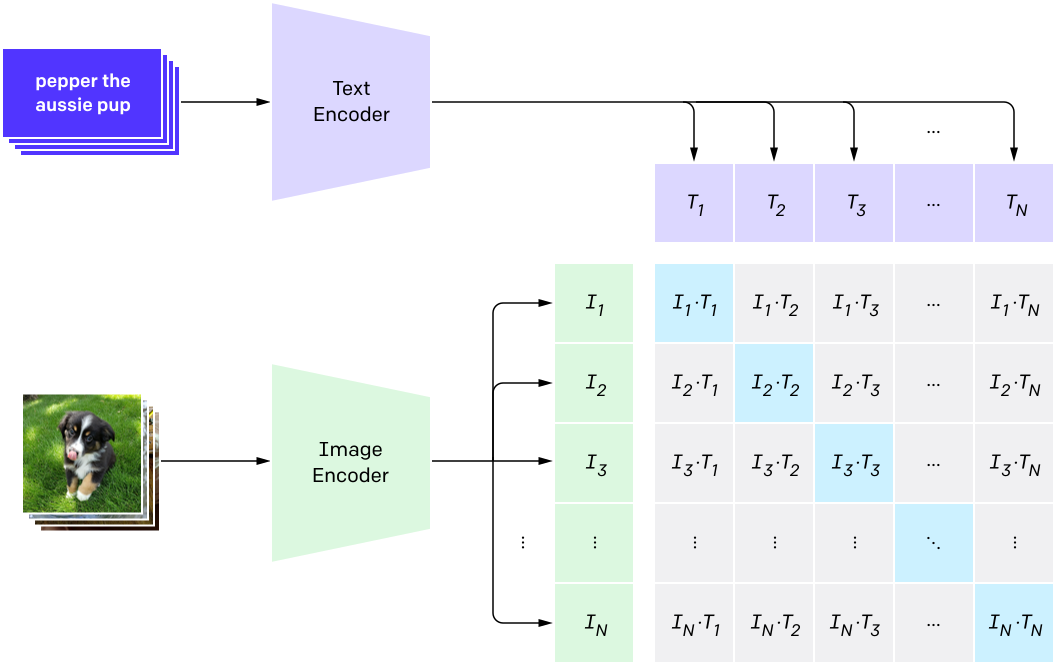
\includegraphics[width=1\linewidth]{figures/02-04-text-support-img/contrastive-pre-training} 

}

\caption{Visualization of a contrastive objective \citep{radford2021learning}. After encoding the data, a similarity matrix for the images and texts is computed. The aim is that the N true image-text pairs score high in terms of similarity, while the \(\text{N}^2 - \text{N}\) other possible combinations score low.}\label{fig:contr-viz}
\end{figure}



Contrastive learning can be contrasted with classical predictive learning.
Figure \ref{fig:contr-vs-pred-learn} gives an interesting insight into the choice of space, where goodness of fit is measured.
The exemplary task is to color an image given its B/W version.
Approach (a) first encodes the B/W image and then decodes the interim latent representation to fitting colors.
The goodness of this fit is measured in the output space, meaning the estimated colors are compared to the true colors.
Conversely, approach (b) measures the loss in the representation space.\footnote{Note that contrastive learning easily works with other combinations of modalities than text and image; here B/W and colors.}
A reason for the good performance of contrastive learning could be that, while common prediction losses (e.g., the \(\mathcal{L}_2\) loss) penalize each prediction output dimension independently, approach (b) implies measurement in the intertwined representation space \citep{tian2020contrastive}.

\begin{figure}

{\centering 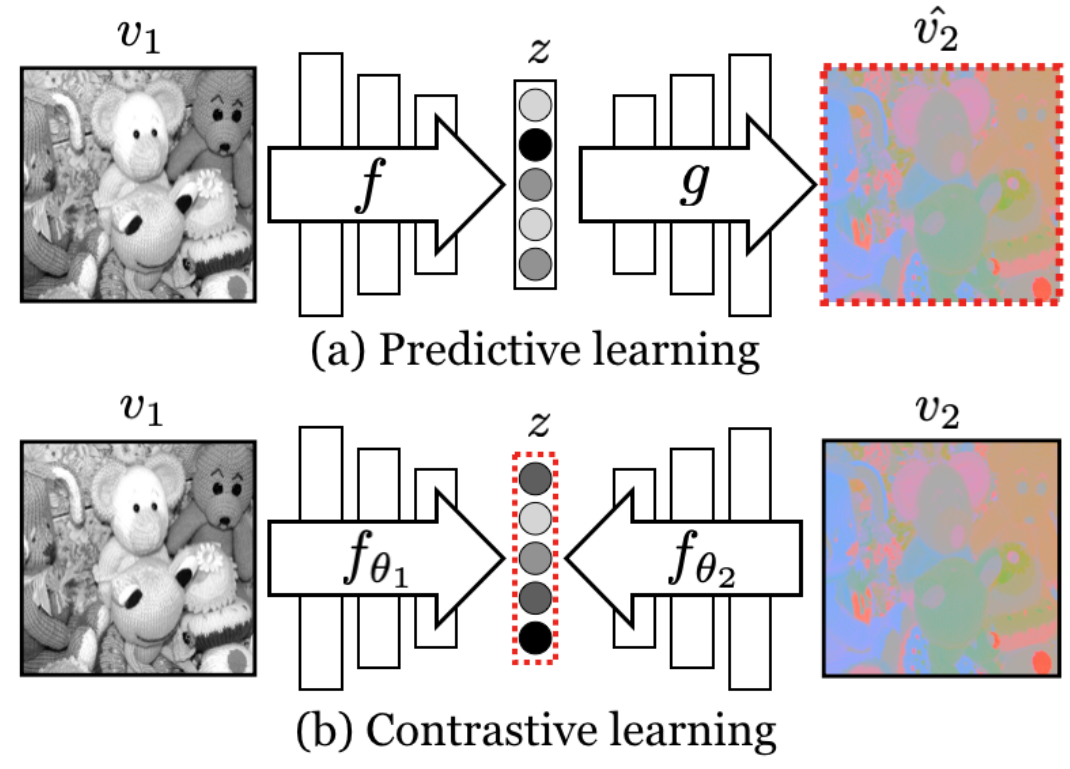
\includegraphics[width=1\linewidth]{figures/02-04-text-support-img/tian-predictive-vs-contrastive} 

}

\caption{Predictive vs.~contrastive learning: Predictive losses are measured in the output space while contrastive losses are measured is in the representation space, indicated by red dotted boxes \citep{tian2020contrastive}.}\label{fig:contr-vs-pred-learn}
\end{figure}



But in the end, rather than theoretical considerations, the driving factor for using this objective is data efficiency.
As can be seen in figure \ref{fig:data-efficiency}, \citet{radford2021learning} start their search for an adequate pre-train model (more on this in subsection \ref{foundMod}) by experimenting with a Transformer-based language model predicting the exact captions of an image.
It turns out that this approach trains three times slower, in terms of data efficiency, compared to a simpler baseline of predicting a bag-of-words text encoding.
Additionally, switching to the contrastive objective of CLIP improves data efficiency by a factor of four.

\begin{figure}

{\centering 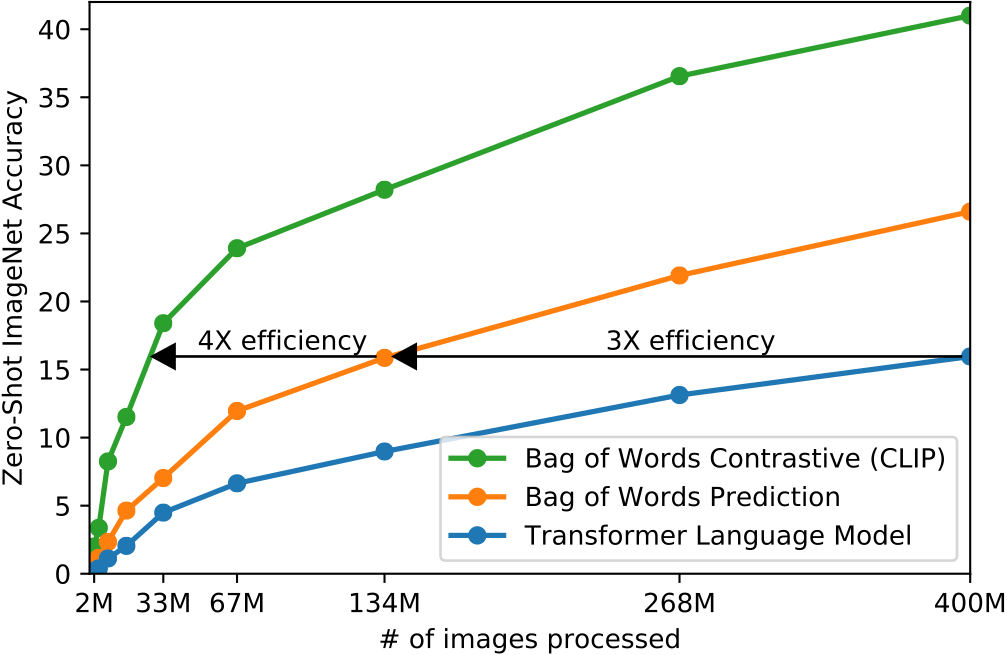
\includegraphics[width=1\linewidth]{figures/02-04-text-support-img/data-efficiency} 

}

\caption{Data efficiency of contrastive objective. Development of zero-shot accuracy (see next subsection \ref{foundMod}) on ImageNet with increasing number of instances of training data seen by models. The contrastive objective reaches same accuracies as the generative approach with only a seventh of the amount of data \citep{radford2021learning}.}\label{fig:data-efficiency}
\end{figure}



Nonetheless, the switch to contrastive learning leads to some limitations.
Its rigidity demands certain extra steps and forfeits the high flexibility of generative models.
In particular, this means contrastive models similar to CLIP are limited to choose from available options and cannot freely generate texts or images.
To extend the capabilities of those models additional network building blocks are necessary.

\hypertarget{foundMod}{%
\subsubsection{Foundation models and zero-shooting}\label{foundMod}}

The first models which are considered foundation models today began to appear in NLP.
The term, later coined by \citet{bommasani2021opportunities}, refers to models that are noteworthy due to their large scale and ability to adapt to a wide variety of downstream tasks.
An early example is BERT \citep{Devlin2018}.
A lot of the time, foundation models have an unfinished touch to them and the true scope of their capabilities cannot be sketched out clearly.
This generally is the case, because the desired abilities of neural networks are not designed for explicitly, but rather emerge during their implementation.
\citet{bommasani2021opportunities} cite GPT-3's ability to perform certain types of new tasks soley by confronting it with the right natural language prompt.
E.g., it is possible to get GPT-3 to summarize a paragraph by appending ``TL;DR'' (too long, didn't read) to the prompt, which is a common pattern on the internet to signal a following summery.
This is called ``in-context learning'' \citep{brown2020language}.
It is apparent that one can make up plenty of unexpected ways to employ these models and it cannot be known whether there is a further way no one thought of yet.
This means possibly saving computational and data collection costs down the line, which ineptly is true for malicious use cases, e.g., surveillance, too.

Foundation models build on the concept of transfer-learning, i.e., pre-training a model on a task that is feasible to do and applying it to the desired task downstream.
In the context of this chapter this means pre-training on web-scale data (see subsection \ref{webScaleData}) and evaluating performance on various common classification datasets.
E.g., \citet{radford2021learning} name the SVHN dataset as a proxy for the task ``street number transcription'' with the caveat ``on the distribution of Google Street View photos'', but they remark that a lot of datasets have no obvious, specific task associated, e.g., CIFAR-10.
They use these kind of datasets for measuring the ``robustness to distribution shift and domain generation'' of their model, which still is a topic of great interest as mentioned in subsection \ref{webScaleData}.
When there is no further fine-tuning on the downstream task, i.e., no resuming of training on the new dataset, this is called zero-shooting.
It has the clear advantage of evaluating performance more unbiased, as processes like overfitting to the data-generating distribution will not distort results.

Figure \ref{fig:zero-shooting} shows how contrastive models perform zero-shot transfer.
In the case of image classification all available classes are encoded by the language model.
Afterwards, the CV sub-network computes the encoding of the image to be classified and all pair-wise similarity scores are returned.
The pair with the best score can be retrieved as the decision.
Image retrieval works the other way around:
After an initial encoding of all images, the ones most similar to the encoded natural language text prompt in the representation space can be returned.

\begin{figure}

{\centering 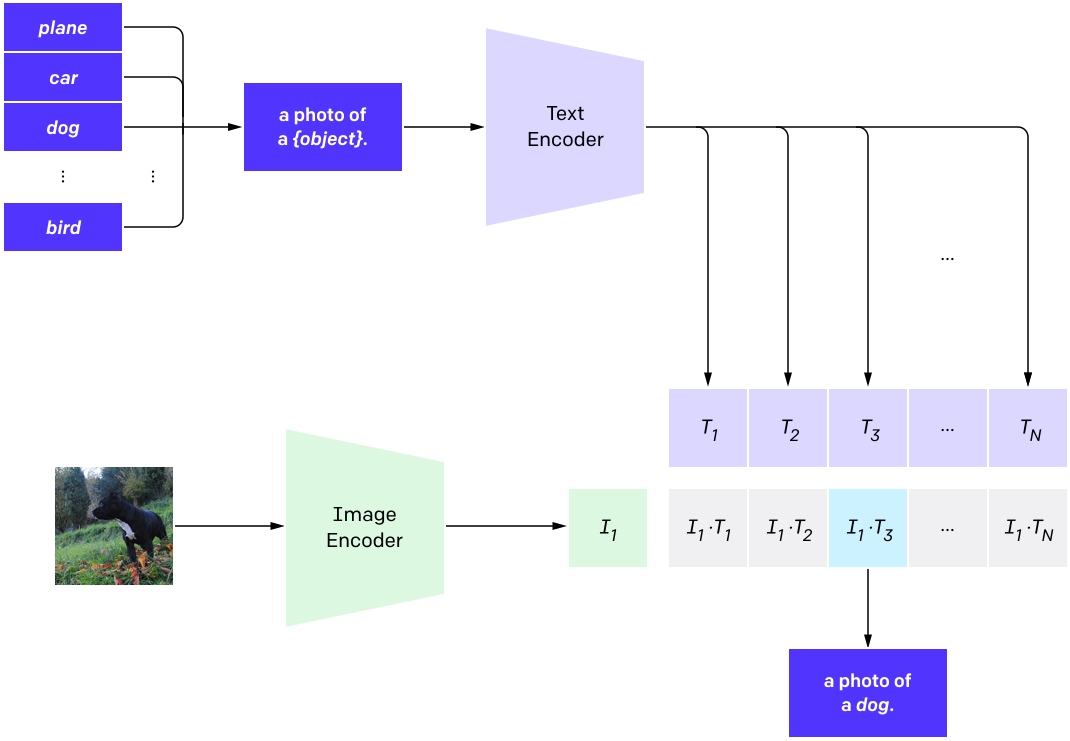
\includegraphics[width=1\linewidth]{figures/02-04-text-support-img/zero-shooting} 

}

\caption{Visualization of zero-shooting \citep{radford2021learning}.}\label{fig:zero-shooting}
\end{figure}



\hypertarget{architectures}{%
\subsection{Architectures}\label{architectures}}

\hypertarget{clip}{%
\subsubsection{CLIP}\label{clip}}

The first of the large scale contrastive CV models that were published is CLIP, short for Contrastive Language-Image Pre-training \citep{radford2021learning}.
The components of its name are explained in previous subsections \ref{contrObj}, \ref{webScaleData} and \ref{foundMod} and are the crucial concepts of ALIGN and Florence as well.
CLIP is a product of OpenAI, but its code is freely available and the different versions can be accessed as \href{https://github.com/openai/CLIP}{python modules}.
Not released is its dataset.

A lot of preliminary work stems from \citet{zhang2020contrastive}, whose paper firstly describes contrastive representation learning using image-text pairs.
Their implementation of the contrastive loss function \eqref{eq:contrLoss} is

\begin{equation}
  \ell_1^{V_\text{img}, V_\text{txt}} = - \log \frac{\exp(\langle v_\text{img}^1, v_\text{txt}^1 \rangle / \tau)}{\sum_{k=1}^{N} \exp(\langle v_\text{img}^1, v_\text{txt}^k \rangle / \tau)},
  \label{eq:contrLossCLIP}
\end{equation}

where \(\langle v_\text{img}^1, v_\text{txt}^1 \rangle\) represents the cosine similarity, i.e., \(v_\text{img}^{1 \top} v_\text{txt}^1 / (\|v_\text{img}^1\| \|v_\text{txt}^1\|)\), and \(\tau \in \mathbb{R}^+\) is a temperature parameter, which is directly learned during training \citep{zhang2020contrastive}.
CLIP adopts this.
\(\ell_1^{V_\text{txt}, V_\text{img}}\), the counterpart to \(\ell_1^{V_\text{img}, V_\text{txt}}\) for the total loss, is function \eqref{eq:contrLossCLIP} with switched arguments.
This can be viewed as a symmetric cross entropy loss over the cosine similarity of the embeddings \citep{radford2021learning}.

\textbf{Architecture}

The text encoder for CLIP (see figure \ref{fig:contr-vs-pred-learn}) is a modified Transformer \citep{vaswani2017attention}, which was also used for GPT-2 \citep{radford2019language}.
For the image encoder multiple sub-networks are tested:

\begin{itemize}
\tightlist
\item
  ResNets: ResNet-50, ResNet-101
\item
  ResNets which follow EfficientNet-style model scaling: RN50x4, RN50x16, RN50x64
\item
  Vision Transformers: ViT-B/32, ViT-B/16, ViT-L/14
\end{itemize}

The best performing sub-network was the ViT-L/14.
In turn, they trained it for an additional epoch with higher resolution images (336px), denoting this version \href{mailto:ViT-L/14@336px}{\nolinkurl{ViT-L/14@336px}}.
If not indicated otherwise, the performances of this version of CLIP are displayed.
The EfficientNet-style ResNets use x4, x16 and x64 of the compute of a ResNet-50 and the largest model (the RN50x64) trained for 18 days on 592 V100 GPUs, while the ViT-L/14 only took 12 days on 256 GPUs.
The high parallelization capabilities of Transformers seem to pay off.

When explaining zero-shooting initially (see subsection \ref{foundMod}), a text processing step was skipped.
As can be seen in figure \ref{fig:zero-shooting}, there is an additional operation before the labels are fed into the text encoder.
In order to help the model understand the context of the words, the class labels are embedded in a sentence, e.g., ``A photo of a \{label\}.''.
This increases the models zero-shot accuracy on ImageNet by 1.3 percentage points (pp).
When ensembling 80 different context prompts\footnote{Prompts like: ``A photo of a big \{label\}.'', ``A photo of a small \{label\}.'' \citep{radford2021learning}} \citet{radford2021learning} improve ImageNet accuracy by an additional 3.5pp, which adds up to a total of nearly 5pp.
The average performance gain across 36 datasets is reported to be 5pp.
It is likewise possible to directly communicate visual concepts like ``picture'', ``macro'', ``drawing'' or even ``dog'' to the model.

\textbf{Robustness}

Figure \ref{fig:performance-clip} reports the performance of CLIP and a ResNet101, whose training on ImageNet was stopped at the point it reached the same accuracy as zero-shot CLIP.
It can be deduced that the methods studied in the paper of \citet{radford2021learning} constitute an important step towards closing the robustness gap mentioned earlier (see subsection \ref{webScaleData}).
While the performance of the ResNet101 deteriorates with datasets generated from more and more different data distributions compared to ImageNet, CLIP remains fairly accurate.
Note that these findings have to be taken with a grain of salt.
Because OpenAI does not grant public access to their training data, independent parties cannot investigate these claims on their own.
E.g., it has to be relied on the conclusions of their overlap analysis to rule out that CLIP has not seen biasing amounts of future test data during training.

\begin{figure}

{\centering 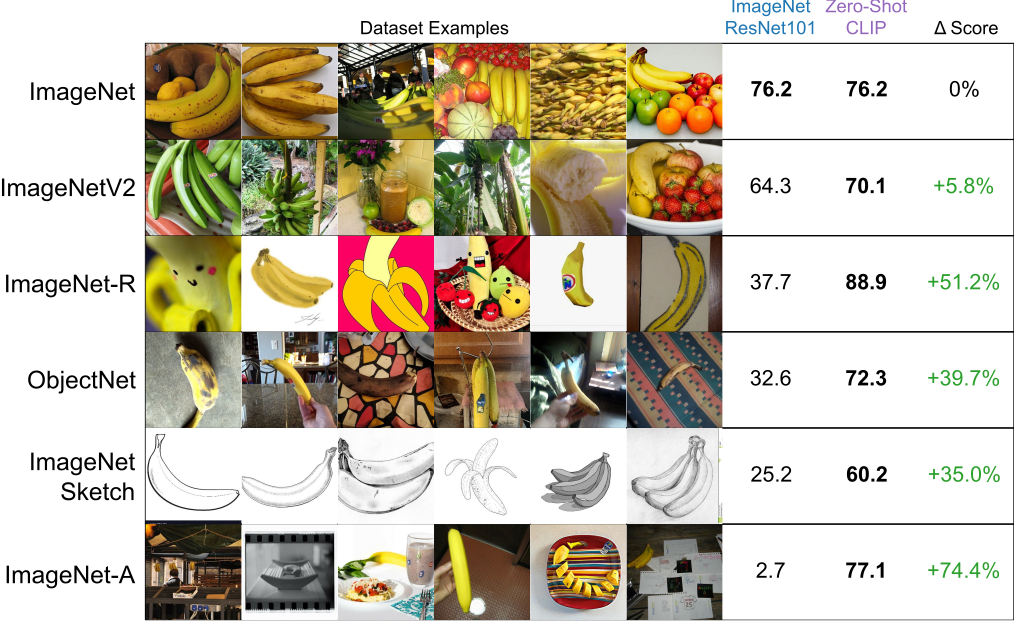
\includegraphics[width=1\linewidth]{figures/02-04-text-support-img/performance-clip} 

}

\caption{Robustness of zero-shot CLIP to distribution shifts \citep{radford2021learning}.}\label{fig:performance-clip}
\end{figure}



\textbf{CLIP as a building block}

\citet{shen2021much} study how the performance of Vision-and-Language (V\&L) models improves, when the visual encoder is switched to CLIP's strong image encoder.
They discover that in this field of CV the ViT-B scores significantly worse than the ResNets.
E.g., tests on image captioning reveal that the V\&L model using ViT-B often performs only half as strong as the version using the RN50x4 (the largest network used in this study).
This is possibly due to the pooling strategies of ViT-B, which result in a lack of visual localization abilities.
\citet{shen2021much} test their hypothesis and generate, e.g., figure \ref{fig:attention-ViT} which depicts Grad-CAM Visualizations for a V\&L model with a ViT-B backbone and a ResNet-50 backbone and the question ``What color is the woman's shirt on the left?''.
The red area indicates relevant pixels and appears much more focused for CLIP-Res50 than for CLIP-ViT-B.

\begin{figure}

{\centering 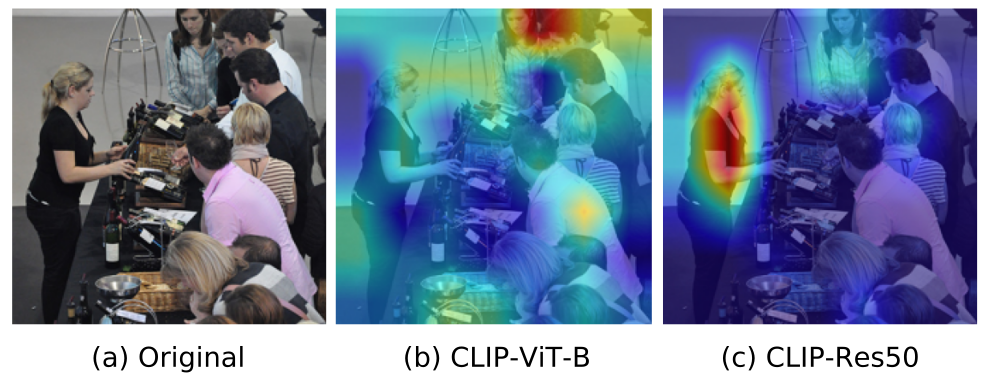
\includegraphics[width=1\linewidth]{figures/02-04-text-support-img/attention-of-ViT} 

}

\caption{Grad-CAM Visualizations for the prompt ``What color is the woman's shirt on the left?''.}\label{fig:attention-ViT}
\end{figure}



\hypertarget{align}{%
\subsubsection{ALIGN}\label{align}}

The approach of \citet{jia2021scaling} is largely similar to CLIP.
They reiterate the necessity of large-scale vision datasets, but assert that even CLIP's data collection process still involves a non-trivial amount of data curation.
They propose that the amount of additional observations obtained through minimizing the amount of filtering makes up for the increased noise.
The result is a dataset with 1.8 billion image-text pairs.
The corresponding model is named ALIGN, short for ``A Large-scale ImaGe and Noisy-text embedding'', whose acronym hints at the contrastive loss, which aligns vector encodings in the representation space (see subsection \ref{contrObj}).

\textbf{Architecture}

ALIGN follows the dual encoder architecture employed by \citet{zhang2020contrastive} and \citet{radford2021learning}, but uses part of BERT-Large as the text and EfficientNet-L2 as the image encoder, which they jointly train from scratch.
The model has around 800 million parameters \citep{alford2021alignparams}.
Subsection \ref{performanceComp} goes into more detail about the performance of ALIGN and compares all three models discussed in this subsection.

\textbf{Connecting image and text representations}

The contrastive loss function aligns the latent representations of the different modalities.
In other words, the explicit objective is that similar vector encodings implicate similar inputs.
This means arithmetic operations like the ones mentioned in chapter \ref{c01-01-sota-nlp} are not only meaningful on encodings belonging to the same modality, but to different modalities.
E.g., one can add up the image encoding of a picture of the Eiffel tower and the text encoding of the word ``snow'' and retrieve pictures with high cosine similarity to the result, see figure \ref{fig:img-txt-addition}.

\begin{figure}

{\centering 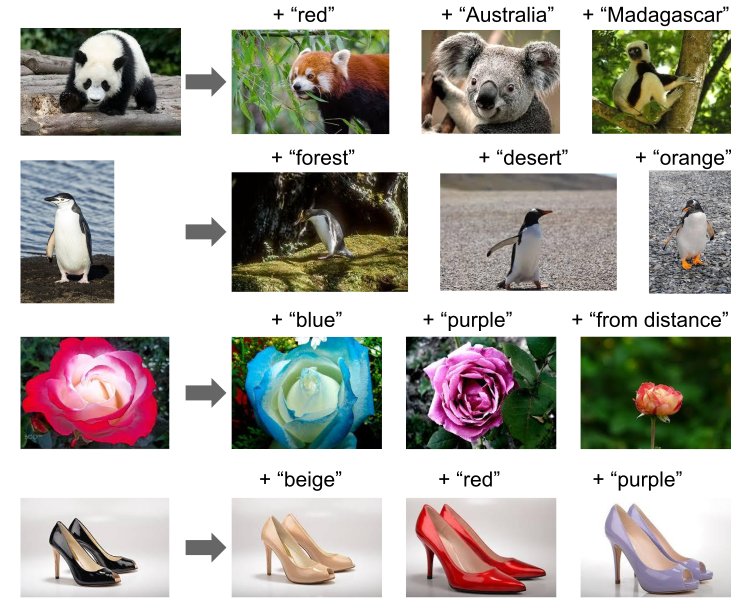
\includegraphics[width=1\linewidth]{figures/02-04-text-support-img/align-word-and-image-addition} 

}

\caption{Multimodal image retrieval via arithmetic operations on word and image embeddings.}\label{fig:img-txt-addition}
\end{figure}



\hypertarget{florence}{%
\subsubsection{Florence}\label{florence}}

While in principle the approach of \citet{yuan2021florence} does not largely differ from the others, the focus of this paper is more about making a true foundation model.
In order to achieve this, they propose a map of possible vision applications which the try to cover via extending the core model with modules.
As figure \ref{fig:florence-dimensions} depicts, they want to advance into the dimensions of fine-grained object detection, dynamic action recognition and true multimodal tasks.
Because of their big ambitions, they name their model Florence after ``the birthplace of Renaissance'' \citep{yuan2021florence}.

\begin{figure}

{\centering 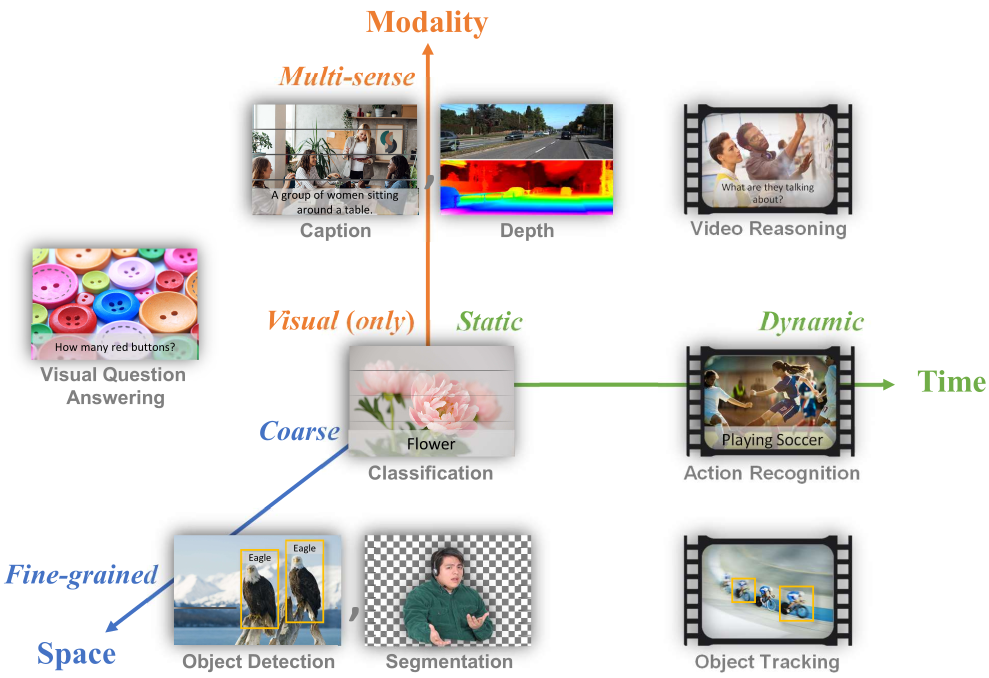
\includegraphics[width=1\linewidth]{figures/02-04-text-support-img/florence-dimensions} 

}

\caption{Florence' approach to foundation models: A general purpose vision system for all tasks.}\label{fig:florence-dimensions}
\end{figure}



\textbf{Architecture}

For the two encoders of the pre-trained core they use a hierarchical Vision Transformer (CoSwin Transformer) for images and a Transformer similar to CLIP's for text.
Their 893 million parameters are also jointly trained from scratch on 900 million image-text pairs.
The alignment happens in the so called image-label-description space which is encoded through a special version of the contrastive loss function which regards all image-text pairs with the same label as positive instances.
Figure \ref{fig:florence-architecture} depicts their version of figure \ref{fig:contr-viz} where one can schematically see how they flexibly add modules to the pre-trained core in order to adapt to various downstream tasks.

\begin{figure}

{\centering 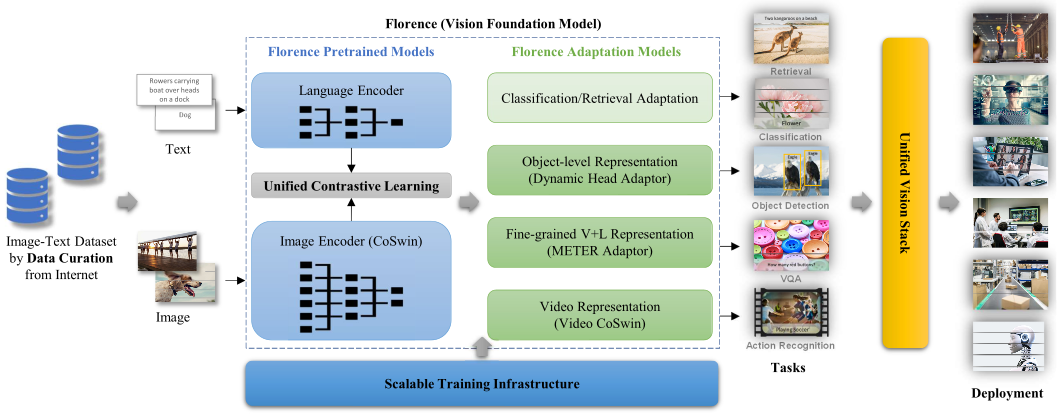
\includegraphics[width=1\linewidth]{figures/02-04-text-support-img/florence-architecture} 

}

\caption{Modular architecture of Florence.}\label{fig:florence-architecture}
\end{figure}



\hypertarget{performanceComp}{%
\subsection{Performance comparison}\label{performanceComp}}

Throughout the papers of \citet{radford2021learning}, \citet{jia2021scaling} and \citet{yuan2021florence} is was possible the collect three tables with reported performance measures.

Table \ref{fig:table1} summarizes the zero-shot accuracies on four different ImageNet variants.
Unfortunately \citet{yuan2021florence} only stated their performance on the original ImageNet, where they beat CLIP and ALIGN by a margin of 7.3pp.
The results on the other three ImageNet pendants are mixed and there is no clear winner between CLIP and ALIGN.

\begin{figure}

{\centering 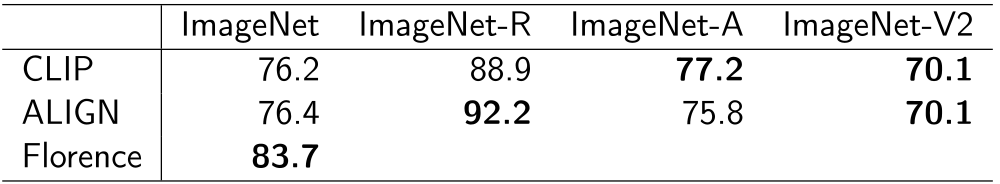
\includegraphics[width=1\linewidth]{figures/02-04-text-support-img/table-imagenet} 

}

\caption{Top-1 Accuracy of zero-shot transfer of models to image classification on ImageNet and its variants.}\label{fig:table1}
\end{figure}



Table \ref{fig:table2} concerns zero-shot image retrieval on the Flickr30K and the MSCOCO dataset (see chapter \ref{c01-03-benchmarks}).
Even though there are not many major score differences, there is a clear ranking with CLIP on third, ALIGN on second and Florence on first place.

\begin{figure}

{\centering 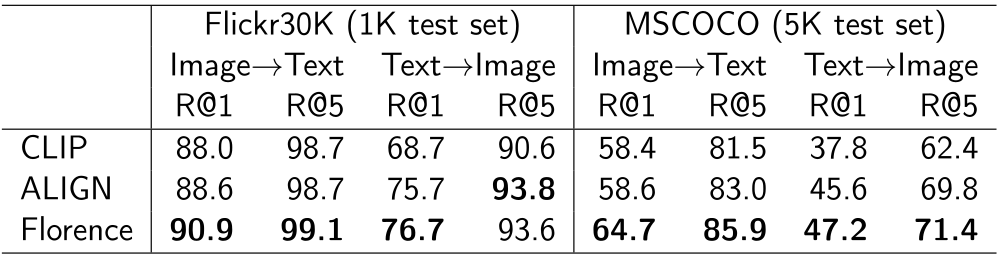
\includegraphics[width=1\linewidth]{figures/02-04-text-support-img/table-img-txt-retrieval} 

}

\caption{Zero-shot image and text retrieval \citep{yuan2021florence}.}\label{fig:table2}
\end{figure}



The most comprehensive comparison is comprised in table \ref{fig:table3}.
It depicts the accuracy of zero-shot CLIP and Florence on various datasets as well as the scores of all three models fine tuned to the respective datasets.
Florence beats CLIP in nearly all evaluations, for the zero-shot setting as well as for fine tuned performance.
\citet{jia2021scaling} only report on four of the twelve dataset, where they lead half of the time.

\begin{figure}

{\centering 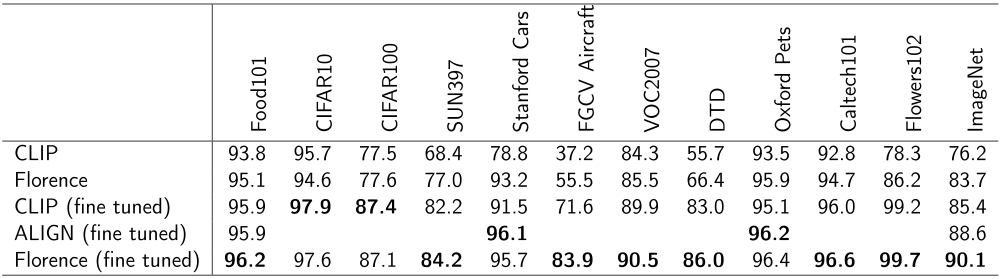
\includegraphics[width=1\linewidth]{figures/02-04-text-support-img/table-misc-datasets} 

}

\caption{Top-1 Accuracy of CLIP, Florence and ALIGN on various datasets.}\label{fig:table3}
\end{figure}



Summing up, ALIGN achieves its goal of replicating CLIP's impressive performance while dramatically reducing data curation efforts and Florence has the overall top performance.
This could be attributed to its custom loss, maybe to \citet{yuan2021florence} striking the best balance between sample size and data curation or to Florence having the best sub-networks; or a combination of all three.

Once again note that none of the training datasets were made publicly available.
It cannot be guaranteed that all benchmarks were evaluated on unseen datasets.

\hypertarget{resources}{%
\subsection{Resources}\label{resources}}

One can access the pre-trained CLIP models on \href{https://github.com/openai/CLIP}{Github} and they even found their way into simple command line tools already.
For example there is a CLI named \href{https://github.com/yurijmikhalevich/rclip}{rclip}, which can be used for personal image retrieval, wrapping the \emph{ViT-B/32} CLIP architecture.
On my (mid-range) laptop I was able to find seemingly good matches for search terms which I tried out inside a folder containing about 100 pictures.
After an initial caching one request took about ten seconds.
Furthermore CLIP continues to be used inside new models, e.g., DALL\(\cdot\)E 2, where it is responsible for image embedding \citep{ramesh2022hierarchical}.
Also, there is an effort to replicate CLIP's training dataset called LAION-400M \citep{schuhmann2022laion}.
To validate the image-text pairs collected for this, their cosine similarity is computed using CLIP and instances with a value too low are discarded.
As to my knowledge nothing was made publicly available as part of the other two papers.

\hypertarget{c02-05-text-plus-img}{%
\section{Text + Image}\label{c02-05-text-plus-img}}

\emph{Author: Steffen Jauch-Walser }

\emph{Supervisor: Daniel Schalk}

Data is naturally at the heart of every data scientific issue. While there have been many advances made in machine learning in recent years, many promising research areas remain, as do a multitude of problems associated with them. One such promising area are multi-modal machine learning models.
Combining different input data is a key aspect towards making models more sophisticated. When thinking about teaching robots specific tasks, detecting hateful memes or deep fakes, it is apparent that only through the combination of multiple modalities, success might be achieved. Context is key.

However, learning context requires increasingly complex models.
While early machine learning models built their success upon the possibility to analyze the big pool of available, often unstructured data, modern machine learning models are so demanding that there is often not enough data or training time available.
Obtaining data is a major issue for multi-modal machine learning. Since labelling data in vast amounts is prohibitively expensive, larger models have to come up with specific strategies to move forward such as self-supervised training or automatically scraped web datasets. Nevertheless, when models become so large that billions of parameters have to be learned, even scraping the whole web starts to show its limits. Another natural issue is the transformation of different types of data into usable model inputs.

There is no shortage of different single modality machine learning models.
On the contrary, when every new hyperparameter configuration might be seen a new model, it becomes hard to keep track. More importantly, it is often not clear how a model from one area transfers to another. Did we learn some modality specific bias or a general principle? Consolidating different models into a unifying framework is a key prospect of multimodal machine learning. While the grand dream of a single unifying model might be out of reach, consolidating different areas
is well in sight.
In the following, we will have a look at the challenges and prospects of multimodal machine learning against the background of visual language models. Visual Language Models are models which can deal with both language and images as input data. Specifically, we will have a closer look at three different models: Data2vec,VilBert and Flamingo. Data2vec is an unsupervised
model that can handle different modalities, but not their interaction, using a single unifying training framework. VilBert is an early visual-language model that can and handle interactions between images and text through its innovative concept of cross-attention. Flamingo is a recent few shot visual language model that features large expressive text capabilities through the use of a large langue model. With 80B parameters, it particularly highlights how to leverage the communication between frozen models when further scaling up the model size.

An overview across the popularity of current research fields in visual language modelling is provided in figure \ref{fig:vltasks}. A detailed list of trends for each of those fields can be found in the accompanying paper (\citet{uppal2022multimodal}). Most research is done in the
areas of visual question answering (VQA) and visual captioning (VC), but also for example visual commensense reasoning (VCR), vision-language navigation (VLN) or multimodal affective computing (MAC). MAC uses images and text to infer sentiment, for example through facial expressions. VCR as an extension of VQA is particularly interesting in the realm of making models more interpretable.
After all, we would like to know why machine learning models do what they do. Finally, VLN has many promising practical applications in the field of robotics, particularly the interaction of humans and robots.

\begin{figure}

{\centering 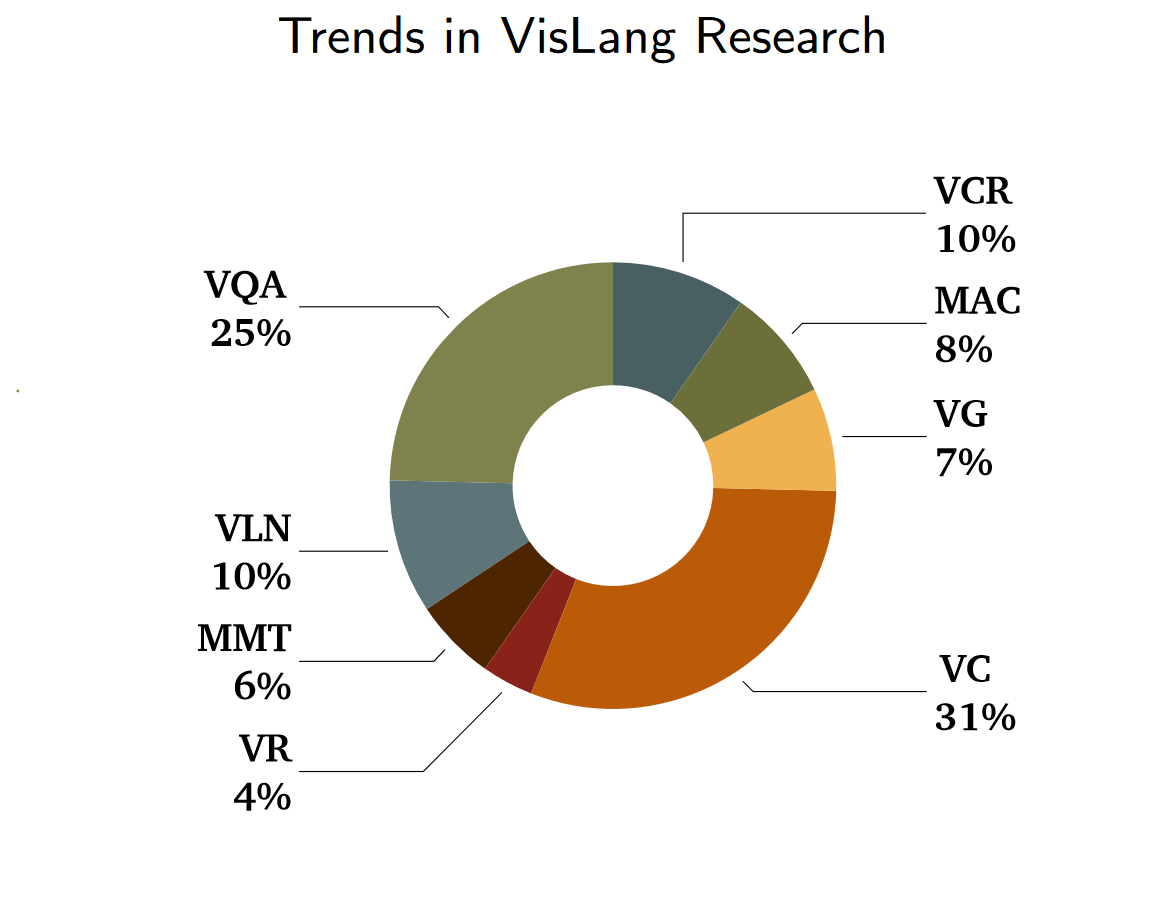
\includegraphics[width=0.7\linewidth]{figures/05-chapter2/vltasks} 

}

\caption{Uppal et al. (2022): VisLang Paper Trends (previous 2 years)}\label{fig:vltasks}
\end{figure}

\hypertarget{data2vec}{%
\subsection{Data2vec}\label{data2vec}}

With data2vec (\citet{baevski2022data2vec}), data scientists at Meta, formerly Facebook, developed an architecture that addresses some of the mentioned issues while highlighting the importance of sophisticated training schemes. Their algorithmic structure is able to work with either text, image or speech data. On top of that, the model is self-supervised based on a teacher-student relationship which reduces the need for human labelling. It is not a universal model in the sense that it works with any input, nor is it even a general model in the sense that the algorithm is exactly the same for each modality. However, the overall model structure remains the same for either text, speech or image input data, while only the specific encoding, normalization and masking strategies are modality-specific. In that regard, it is a step towards a more general way of dealing with different modalities and it is very effective at doing so given the benchmark results on typical data sets. Particularly noteworthy is also the way they implement the self-supervised learning. Data2vec predicts contextualized and continuous representations rather than typically used discrete tokens such as sub-words. Working with latent representations of the input space has two advantages: not only is the number of prediction targets not a-priori limited, but they are also richer in information.

\begin{figure}

{\centering \includegraphics[width=1\linewidth]{figures/05-chapter2/datavecoverview} 

}

\caption{Baevski et al. (2022): Data2vec Architecture - a teacher model creates contextualized latent targets on the basis of its top K layers (blue) as prediction task to train the student model}\label{fig:data2vecoverview}
\end{figure}

Figure \ref{fig:data2vecoverview} depicts the general model architecture. The two main components are a teacher and a student model which only differ in one aspect, the weights of the teacher model are an exponentially decaying average of the student's weights. The purpose of the teacher model is to create training targets for the student model.
In a first step, a modality is chosen and inputs are encoded according to the specific encoding scheme for that modality. A masked version is given to student model, but notably, the teacher model has access to an unmasked, complete view of the input data. Hence, the resulting training targets will be fully contextualized using a self-attention mechanism over the whole input data. The training targets are based on the top K layers of the teacher model depicted in blue in \ref{fig:data2vecoverview} . More specifically, denote by \(y_t\) the training target at time t and by \(a_t^l\) the outputs of the l-th block, then \(y_t = \frac{1}{K}\sum_{l=L-K+1}^{L} \hat{a}_t^l\), i.e.~the training targets are the average of the outputs of the top K layers of the teacher network after a normalization has been applied. Normalization helps to stabilize the training process and prevent model collapse which can be an issue with models that learn their own representation.

From the authors point of view, working with a latent representation of the actual learner as training target is a simplification of many commonly used modality-specific designs despite the caveat that this paper still uses modality-specific encoding strategies. Compared to other models, there is no cross-modality training. The specific loss function used to regress the targets is a smooth L1 loss.

\begin{align*}
       L(y_t,f_t(x)) =
    \begin{cases}
        \frac{(y_t - f_t(x))^2}{\beta}    \quad &\text{if} \quad | (y_t - f_t(x)) | \leq \beta \\
                | (y_t - f_t(x) | - \frac{\beta}{2} \quad &\text{otherwise}
    \end{cases}
\end{align*}

Using a smooth L1 loss has the advantage of being continuous, yet sensitive to outliers, however the \(\beta\) parameter needs tuning.
As far as the general model architecture is concerned, the underlying architecture is a standard transformer architecture (\citet{vaswani2017attention}).

How does the modality specific input handling work?
In many ways, in this work the authors combine the strategies developed in multiple previous works and add a unifying framework on top of it. For images, the typical Vision Transformer (ViT) strategy (\ref{fig:visiontransformer}) to transform images with a size of 224x224 pixels into 16x16 pixel patches is employed. Every patch is then linearly transformed into a sequence of 196 flattened representations including a learnable positional encoding that serve as input to the vision transformer. A classification token is used to produce the final categorization. The contextualization is produced in the multi-head attention blocks as explained in earlier chapters.
In short, multi-head attention first projects the keys, queries and values with learned linear projections which are then evaluated in parallel to create more expressive attention maps. Attention itself is calculated as scaled dot-product-attention using a softmax over the scaled product of keys, queries and values.(\citet{vaswani2017attention})
As far as the vision transformer itself is concerned, datav2vec tests two different model sizes, a base model size of 12 and a large model of 24 transformer blocks. The masking strategy for images follows the Bert pretraining approach of image transformers, BEiT, proposed by (\citet{bao2021beit}). In particular, multiple adjacent blocks are being masked with random aspect ratio. The minimum size of a masked block is 16 patches. In total, 60\% of patches were masked in the data2vec algorithm, which is an increase over the original 40\% used by BEiT. However, the authors note that they found increased masking to be more accurate. The augmentation strategies are similar, as well. Resizing crops, horizontal flipping and colour jittering were used. Naturally, the student and teacher model are the given the same modified image. Finally, for image data, the model is measured on a classification task. Hence, the authors use a mean-pooling over all patches in the last transformer block and input that into a softmax-normalized projection that conducts the classification, which is again based on the BEiT model.

\begin{figure}

{\centering \includegraphics[width=1\linewidth]{figures/05-chapter2/visiontransformer} 

}

\caption{Dosovitskiy et al. (2021)}\label{fig:visiontransformer}
\end{figure}

The natural language processing model is implemented with a PyTorch toolkit named fairseq and based on the RoBERTa (\citet{liu2019roberta}) architecture which redesigned the standard Bert model training procedure to make it more robust and effective. In particular,
it increases hyperparameters such as the learning rate and the batch size. It also removes the next sentence prediction task to improve on the masked language modelling performance.
In this case they follow (\citet{sennrich2015neural}) and encode sub-words as 50k byte-pairs. A separate embedding vector is learned for each type. For the masking, the Bert masking is being used. 15\% of the embedded tokens are replaced,
thereof 80 percent are learned masks, 10\% are unchanged and the remaining 10\% are replaced with random tokens in the vocabulary. Another strategy that the authors also consider is the wave2vec masking strategy
to mask four consecutive tokens with a probility of 0.35 while only using learned tokens (\citet{baevski2020wav2vec}). As it turns out, the later strategy further improves results. The natural language processing model is evaluated on
the General Language Understanding Evaluation (GLUE) benchmark (\citet{wang2018glue}) which includes for example includes NLP inference, sentence similarity and sentiment analysis tasks.

The speech category is also implemented in fairseq. The feature encoder for speech is based on the wave2vec framework and uses 16kHz inputs. It is built upon seven temporal convolutions intertwined with normalization layers
and a GELU activation function such that the output of the encoder is 50 kHz.

As far as the results are concerend, data2vec achieved state-of-the-art performance in vision and language tasks among similar self-supervised models.

\begin{figure}

{\centering \includegraphics[width=0.5\linewidth]{figures/05-chapter2/datavecresultsone} 

}

\caption{Baevski et al. (2022): data2vec performance (vision)}\label{fig:data2vecresults1}
\end{figure}

Figure \ref{fig:data2vecresults1} shows the model's performance in computer vision.
Pretrained and fine-tuned simply on the data of the well known ImageNet-1K dataset,
data2vec was evaluated using top1-accuracy, the standard notion of accuracy, on the task to
predict single labels for images. The base model ViT-B comprises 86M parameteres and ViT-L 307M parameters. The results show that predicting contextualized latent representations in a masked
prediction setup can work well as model training compared to classical local methods such as predicting visual tokens.
MoCov3 (\citet{chen2021empirical}) is a self-supervised model trained on a contrastive loss. The most similar model is DINO (\citet{caron2021emerging}), which also uses a self-destillation setup to predict teacher outputs using a cross-entropy loss. However, their predicition target was the final layer rather than averaged layers while using differing images for teacher and student network. The well performing MAE model (\citet{he2022masked}) is a masked autoencoder which is trained on reconstructing masked pixels using an asymmetric encoder-decoder architecture. In contrast, MaskFeat (\citet{wei2022masked}) uses masked feature prediction. Notably, data2vec outperforms all of them although trained for the same amount or less. Particularly, MAE and MaskFeat use 1600 epochs rather than 800 like data2vec.

\begin{figure}

{\centering \includegraphics[width=1\linewidth]{figures/05-chapter2/datavecresultstwo} 

}

\caption{Baevski et al. (2022): data2vec results (language)}\label{fig:data2vecresults2}
\end{figure}

Figure \ref{fig:data2vecresults2} shows the performance in the language domain.
For the language domain, the model is evaluated on the GLUE benchmark (\citet{wang2018glue}).
The model is pretained and fine-tuned seperately on the labelled data from each task. Acurracy
is reported as the average across 5 tuning cycles. While data2vec achieves a higher average performance than the baseline model, there are tasks
where the baseline model prevails. A large portion of the peformance difference seems to be driven
by the CoLA task. The Corpus of Linguistic Acceptability (CoLA) consists of 10657 sentences from 23 linguistics publications and the task is to judge whether they are grammatically correct. Hence, it is distinctly different from the other tasks. The Stanford Sentiment Treebank (SST) analyzes sentiment in language through movie reviews. The Multi-Genre Natural Language Inference (MultiNLI) corpus contains sentence pairs and focusses on
textual entailment across genres. Similar tasks are used in the Recognizing Textual Entailment (RTE) dataset which focuses on text from news and wikipedia. The QNLI (Question-answering NLI) dataset is a Natural Language Inference dataset that contains answers from wikipedia to corresponding questions posed by an annotator. The task for the model is to find out whether the sentence contains the answer to the question. QQP stands for Quora Question Pairs, which analyzes paraphrases. Finally, the Microsoft Research Paraphrase Corpus (MRPC) also consists of sentence pairs from newswires which may or may not be paraphrases of each other.

As a suitable baseline model, the authors retrain RoBERTa in the respective setup. On top of the heterogenous performance across language tasks, the evaluation also clearly shows that averaging over multiple layers to create prediction targets improves performance across all three domains. The effects seem to be most pronounced on NLP tasks whereas CV does not benefit from averaging more than three layers. In the speech domain, six layers seems to be enough to reach peak performance.
In any case, performance loss while following the strategy to simply average the maximum amount of layers, rather than fine-tuning K, seems small enough to be potentially acceptable.

To sum it up, data2vec is a self-supervised model that can work with either text, speech or image data, but not across modalities. It aims at unifying the learning framework through a teacher-student-setup that allows for contextualized latent target prediction. The teacher model is based on a complete view of the input data, which introduces contextualization, while the student model only sees a masked version of the input. Compared to previous work, the authors average the top K layers rather than only the final layer of the model, which has a notable effect as shown in \ref{fig:data2vecresults2}. As there are different layers in the transformer network, the authors also investigate which layers work best for prediction. They conclude that the output of the feedforward layer works best. Built on a transformer architecture, self-attention
is the main driver that creates contextualized targets in the teacher model and hence performance.
The authors also show that contextualization through the teacher model works best with the complete view of the input rather than a partial view. On top of not being able to work across modalities, one drawback is that the model's structure still uses modality specific encoding and masking schemes. In that regard, the perceiver architecture (\citet{jaegle2021perceiver}) for example used in the Flamingo model is a complementary approach worth exploring. An earlier model that works across modalities is VilBert.

\hypertarget{vision-and-language-bert-vilbert}{%
\subsection{Vision-and-Language Bert (VilBert)}\label{vision-and-language-bert-vilbert}}

As seen in the previous section, data2vec can handle text, image or speech as input data. However, it cannot do so at the same time. The model's focus is on unifying the training approach rather than working across modalities.
However, when we think about multimodal models, we usually think of working with different modalities at the same time. VilBert (\citet{lu2019vilbert}) is a natural extension of the iconic Bert architecture (\citet{devlin2018bert}) to vision-and-language modelling. An immediate question is whether vision and language inputs should be handled together in a single stream or in parallel. As we will see, it turns out that encoding inputs in parallel and working with parallel streams increases performance.
At heart of that architecture is a co-attention mechanism which enables information exchange between both modalities.

\begin{figure}

{\centering \includegraphics[width=1\linewidth]{figures/05-chapter2/vilbertarc} 

}

\caption{Lu et al. (2019): VilBert's Dual Stream Architecture: dashed transformer modules can be repeated, co-attention modules allow sparse interaction between modalities.}\label{fig:vilbertarc}
\end{figure}

Figure \ref{fig:vilbertarc} shows the employed parallel stream architecture.
Each modality is handled separately and fed into two Bert-style transformer models. This allows for both modalities to be handled according to their respective needs while co-attention layers allow for communication between the streams. For the language stream, the encoding uses the vocabulary plus a special classification token (cls), a sentence separation token (sep) and a masking token (mask). For the vision stream, image region features are extracted via a Faster R-CNN (\citet{ren2015faster}) model which was pretrained on the Visual Genome Dataset (\citet{krishnavisualgenome}). Since image regions lack a natural ordering, its spatial location has to be encoded, as well. VilBert achieves that through a five dimensional vector that encapsulates the image coordinates and the fraction of the covered image area. Through projection, the dimensions of the positional encoding and visual features are matched and then summed. The image token marks the beginning of such an image region sequence while representing the whole image.

Through the dual stream architecture, the complexity of the model can be adjusted separately for each modality. An alternative approach would have to discretize the visual space via clustering and then use the resulting tokens in the same way as text tokens. The drawbacks of that approach are the potential loss of detail at the discretization stage and the loss of flexibility across modalities as a result of the same processing. Finally, a single stream architecture can interfer with pretaining of the language models. The model will have to be fine-tuned based on the created visual tokens. As those might be very different from the text tokens, there is potential for the pretained language model to be become `damaged' in the process and lose capabilities - and idea that is also central to the Flamingo model presented later on.

\begin{figure}

{\centering \includegraphics[width=1\linewidth]{figures/05-chapter2/vilbertattention} 

}

\caption{Lu et al. (2019): Cross-Attention in VilBert}\label{fig:vilbertattention}
\end{figure}

The key innovation in the Vilbert paper (\citet{lu2019vilbert}) is the use of co-attention layers.
In figure \ref{fig:vilbertattention}, the basic architecture is depicted. The co-attention module computes query, key and value matrices in a standard transformer attention fashion. However, it then feeds the keys and values from each modality
into the other modalities multi-head-attention block. As a result, the visual attention will be conditioned on text whereas the language attention will be image-conditioned. This communication between streams only occurs at
specific sections in the model, denoted by co-trm in figure \ref{fig:vilbertarc}. Notably, the language stream features a lot more preprocessing before the first co-attention layer than the image stream.

An interesting question to ask is what is actually learned in those attention layers and how they correspond to human attention maps. (\citet{sikarwar2022efficacy}) analyze the efficacy of co-attention layers for VQA tasks in a VilBert network. Specifically, they compute the question conditioned image attention scores and compare them to human attention maps created in experiments. In those experiments, humans are tasked with unblurring specific image regions to answer the same questions one would expect the machine learning model to answer. Such human attention maps are collected in the VQA-HAT dataset (\citet{das2017human}). Rank correlation is used to compare attention maps. (\citet{sikarwar2022efficacy}) find that in a 6 layer network rank correlation plateaus at layer 4 and increases in the number of image regions proposed while encoding the images. Perhaps more surprisingly, they find a minimal influence of semantics on the generation of the attention maps.
Randomly shuffling words in a sentence when testing the model performance barely changes the attention output, which suggests that keywords rather than sentence structures drive the attention output. Note however that while attention maps remained similar, the model's actual performance on answering the questions dropped noticably by approximately 15\% such that it seems clear that coherent sentences are important for the overall VQA task, but not for the attention creation process. What are the keyword that drive cross-attention in VilBert? The evidence provided by the authors clearly shows that nouns are the most influential parts-of-speech when considering attention maps. On top of that, prepositions can sometimes help identify spatial relations. There is also some support for the hypothesis that removing Wh-words such as ``who'' and ``where'' can improve fine-grained attention maps in the final layer which might be worth exploring further as preprocessing for deeper networks. Another approach would be to search for ways to improve the way attention maps are generated by finding ways to include more of the available sentence information. Most notably, however, using object-based region proposals to process images can lead to bottlenecks that can prevent the model from learning sufficiently fine-grained attention maps as shown in figure \ref{fig:vilbertmaps}. Overall, humans are naturally good at VQA tasks. Hence, it is not surprising that attention maps which correlate well with human attention maps also improve model performance.

\begin{figure}

{\centering \includegraphics[width=1\linewidth]{figures/05-chapter2/vilbertmaps} 

}

\caption{Sikarwar et al. (2022): (Left to Right) Picture, Human Attention, 36 Regions, 72 Regions, 108 Regions. Similarity between human and model attention is measured using rank correlation.}\label{fig:vilbertmaps}
\end{figure}

Figure \ref{fig:vilbertmaps} shows that the number of region proposals fed into the model after processing an image affects the ability of the model to produce adequate attention maps. In this particular case the question ``How many fingers is the girl in the black shirt holding up?'' was correctly answered by humans, as well as a VilBert model using 72 or 108 region proposals. It was answered incorrectly when using only 36 region proposals. Note however that in either case, the machine learning model captured the face of the wrong girl. The model using 72 regions also identified the wrong hand despite answering the question correctly. While the 108 region model identifies the correct hand holding up the fingers, it does not seem to prioritize it over the other identified hands in the picture. Hence, the attention maps are sufficiently different from the human attention map which highlights the need to look closer not only at how models are performing, but also into how their performance has been achieved.

As far as the model training is concerned, VilBert is pretained and fine-tuned. The pretaining tasks comprise masked-multi-modal modelling and multi-modal alignment prediction performed on the Conceptual Captions dataset. That dataset contains about 3,1 million usable aligned image-caption pairs, which have been automatically scraped from web images. For the alignment task, the authors create unaligned images by randomly mismatching captions and images. For the masking task, 15\% of the both the visual and language tokens are masked. The task is to reconstruct the mask from the remaining input in a classical Bert fashion. While the text masks are directly regressed like in Bert, the model predicts distributions over semantic classes for the image regions.
This is achieved through minimizing the KL divergence, a measure for the similarity of distributions, between the output distribution of the pretrained model used in feature extraction and the VilBert predictions.

The performance results are depicted in figure \ref{fig:vilbertresults}.

\begin{figure}

{\centering \includegraphics[width=1\linewidth]{figures/05-chapter2/vilbertresults} 

}

\caption{Lu et al. (2019): VilBert Performance}\label{fig:vilbertresults}
\end{figure}

As mentioned before, the dual stream architecture outperforms the single stream architecture. Furthermore, pretraining considerably boosts performace, as does finetuning.
Interestingly, the authors also study the effect of the size of the dataset and effect of the architecture depth. Performance increases monotonically with dataset size, suggesting that performance can be further improved
with more data. The results on the optimal layer depth are task dependent. VQA and Image Retrieval reach peak performance at 6 layers, where a layer denotes a repeatable block as depicted in figure \ref{fig:vilbertarc}. Zero Shot Image retrieval
greatly benefits from even deeper depth. However, the VCR and RefCOCO+ tasks seemingly benefit from shallower models.
The VQA task is based on the VQA 2.0 dataset. Each image must be matched to one of ten answers. Hence, the VQA task is not open-ended, but treated like a classifcation task. To achieve that, the model is amended by two
MLP layers which use the elementwise product of the model-generated img and cls tokens.
The VCR task is also posed as a multiple choice problem with images from movie scences. To fine-tune for the task, questions and answers are concatenated into four different text input and given as model input together with the image.
In the end, four scores are generated accordingly and selected through softmax.
The RefCoCO+ task is a grounding task. An image region has to be selected according to a natural language reference.
Caption-Based Image Retrieval requires the model to find an image that corresponds to a selected caption. The dataset used is the Flickr30k dataset which contains 30 000 pictures with five captions that are of higher quality than the automatically generated captions from web data.

\hypertarget{flamingo}{%
\subsection{Flamingo}\label{flamingo}}

The VilBert model showed one way how to actually combine visual and language inputs. In contrast, data2vec showed how to design an unsupervised model and how influential the actual training process as well as contextualization can be.
A natural question to ask is then is whether we can build a truly multimodal architecture like VilBert that is self-supervised like data2vec or at little task-specific training and how to optimized its training procedure. In particular, both VilBert and data2vec were tested on multiple tasks, but each task needs slight re-adjustments to the model as well as additional fine-tuning. Ideally, a multimodal architecture would not only be efficient in its initial training, but also easily adaptable to different tasks. Finding ways to not only work with different input modalities, but also with different task is crucial towards building a more general AI. A promising approach in that direction is few shot learning. The following section presents Flamingo (\citet{alayrac2022flamingo}), a few shot multimodal architecture developed by Google which comprises key innovations such as handling arbitrarily interleaved vislang sequences as inputs, as well as ways to effectively combine pretained vision-only and language-only models. As such, it is a visually coditioned autoregressive text generation model.

\begin{figure}

{\centering \includegraphics[width=1\linewidth]{figures/05-chapter2/flamingoexamples} 

}

\caption{Alayrac et al. (2022): Flamingo Prompt-Output-Examples}\label{fig:flamingoexamples}
\end{figure}

Figure \ref{fig:flamingoexamples} demonstrates Flamingos capabilities. It can function as chat bot, describe pictures, work with image sequences (videos) and in doing so, simply needs a few prompts.

At the heart of the model is a large language model, Chinchilla (\citet{hoffmann2022training}), with 70B parameters. Large language models such as GPT-3 (\citet{brown2020language}), as their name suggests, can be trained on a large amount of text data which gives them impressive text generative capabilities.
However, multimodal generative modelling presents some specific challenges not present in language-only modelling. First of all, training large language models is expensive. Hence, it is paramount to work with a pretained version, but trying to teach a large language model the means to work with visual inputs, as well, has the potential to deteriorate or destabilize the pretained model. Second, large language models can suffer from memory constraints that are
potentially severely aggravated by simply adding high-dimensional visual data into an input sequence. Third, good generalist capabilities typically require a huge amount of heterogeneous training data. There might not exist
enough labelled image-caption-pair data to successfully accomplish training a capable few shot learning model in the vision-and-language domain.
To train Flamingo, the authors solve these challenges by foremost exploring ways to generate their own web-scraped multimodal data set similar to existing ones in the language-only domain. Furthermore, they use a perceiver architecture (\citet{jaegle2021perceiver}) that resamples inputs into a fixed amount of visual tokens. Finally, the self-attention layers of the language model are kept frozen during training while cross-attention layers are interleaved. A gating
mechanism ensures that those new cross-attention layers do not interfer at model initialization, thereby improving stability and final performance.

\begin{figure}

{\centering \includegraphics[width=1\linewidth]{figures/05-chapter2/flamingoarc} 

}

\caption{Alayrac et al. (2022): Flamingo Model Structure}\label{fig:flamingoarc}
\end{figure}

Figure \ref{fig:flamingoarc} shows the fundamental architecture of Flamingo.
A pretained vision model as well as a pretained language model are frozen. Together they built the cornerstones of the model. The vision model is pretained using a contrastive text-image approach. Its role is to extract
features such as colour, shape, nature and the position of objects - typical semantic spatial features that one would use in querying. The language model is an existing petrained language model. On top of those frozen
parts, the authors add a perceiver-resampler and gated cross-attention layers as learnable architectures. The perceiver-resampler turns the outputs of the vision model into a fix set of visual tokens. Those visual tokens are then used to create cross-attention layers which are interleaved into the frozen language model.
As a result, Flamingo can model the likelihood of some text y interleaved with a sequence of images or videos x as

\[ p(y|x) = \prod_{l=1}^{L} p(y_l | y_{<l}, x_{<l}) .\]

Here, \(y_l\) denotes the language token associated with the input text and \((y,x)_{<l}\) is the set of preceding tokens. Parameterized by the model is \(p\). As shown in the initial figure, one conditions the Flamingo model
simply by giving it an alternating image and text sequence. This is because the attention mechanism only allows text tokens to attend to the previous image, which turned out to work better than alternative schemes. In particular,
this means that the model can generalize to an arbitrary amount of images regardless of the amount of images used in training.

The training was based on multiple different datasets.
The most important one is a Multimodal MassiveWeb datatset (M3M). To generate it, the authors collect images and text from HTML of approximately 43 million webpages. In the process, the position of images relative to the surrounding
text is also identified. Image tags (image) added in plain text signal the original location of images to the model. In addition to that, end of chunk (EoC) tokens before images separate image-text sequences. The embedding of that token is added to the vocabulary of the language model with a random initialization that can later be learnt. Then, it is possible to infer the length of an image-text sequence, which is another piece of derived information.
To give an idea of the scope of the dataset, M3M contains about 182GB of text as well as roughly 185 million images.
The authors pay special attention not to include traditional task-specific datasets curated particularly for machine learning purposes to guarantee the generality of their modelling approach.
As a second important dataset, algined image text pairs are used. In particular, the ALIGN dataset (\citet{jia2021scaling}).The dataset is further augmented with Long Text and Image Pairs (LTIP) as well as Video and Text Pairs (VTP).
The later datasets contain more descriptive captions than ALIGN. Together the process ensures that the available training datasets are sufficiently large and heterogeneous - two key properties necessary to hopefully achieve good few shot performance.

The training objective is to minimize the weighted sum of dataset specific expected negative log likelihood.

\begin{center}\includegraphics[width=0.5\linewidth]{figures/05-chapter2/dataseteq} \end{center}

Each dataset is weighted with a scalar \(\lambda\) as datasets can be of different quality or feature different properties.
Hence, it might be preferable to pay different attention to different datasets. According to the authors, tuning these weights was essential to overall performance. In practice, the optimization works as follows:
a sample batch with visual language sequences from each dataset is used to compute the gradient of the loss in accordance to the weight of the dataset. Importantly, the authors find that it is beneficial to accumulate
the gradients of all datasets before triggering an updating process. Naturally, the actual datasets used to train the models are extremely crucial, as well. In their ablation studies, the authors find that
removing their web-scraped multimodal dataset from the training pool drops model performance as measured across all selected tasks from a score of 68.4 to 46.9. Removing the dataset containing aligned captions and images
drops performance to a score of 56.5 and not accumulating gradients before the updating process decreases performance to 59.7.

Taking a closer look at the model architecture, the two key structures are the perceiver resampler and the attention layers. Figure \ref{fig:perceiver} shows the architecture of the perceiver. (\citet{jaegle2021perceiver})
Before the input data reaches the perceiver, it is processed by the vision encoder - a Normalizer-Free ResNet which is trained with a constrastive loss similar to the well known Clip model (\citet{radford2021learning}) and yields a good trade-off between
performance and efficiency. The output of the vision encoder is a 2D grid which is than flatted before being fed into the perceiver that connects the the vision encoder with the frozen language model. The resampling
performed by the perceiver-resampler is crucial to reduce the complexity of vision-text cross-attention in the next step. This is particularly notable for video inputs. Inside the perceiver, a set
of learned latent queries cross attend to the flattened vision encoder output. The number of outputs generated by the perceiver is equal to the number of learned latent queries. A change the authors make compared
to previous work is to concatenate the keys and values from the latent queries with the keys and values from the flattened features. The ablation studies show that a medium sized perceiver architecture works best with
improvements around two to three score points. Furthermore, a too large architecture can lead to instable trainings in conjunction with large frozen language model. The authors also test the perceiver against a transformer or MLP,
which showed the perceiver to improve performance scores by around three to five points.

\begin{figure}

{\centering \includegraphics[width=0.5\linewidth]{figures/05-chapter2/perceiver} 

}

\caption{Alayrac et al. (2022): Flamingo Perceiver-Resampler}\label{fig:perceiver}
\end{figure}

The main component that turns the frozen large language model into a functioning visual language model are the cross-attention layers depicted in figure \ref{fig:flamingoattention}. The number of layers added controls the number of free parameters and hence
the complexity and expressiveness of the model. Keys and values of those layers are obtained from the visual features output by the perceiver while using language queries. Specifically, gated cross-attention dense layers are used. The layers are dense because the cross-attention layer is followed by a feed forward layer. They are gated because a tanh(\(\alpha\)) gating mechanism is applied between layers. The gating mechanism ensures that the frozen large language model remains stable at initialization through introducing a learnable scalar parameter \(\alpha\) initialized at 0. Without that initialization, training instabilities can occur.
A key question is how many cross-attention layers should be used. For the small Flamingo model with 3B parameters, the ablation studies show that adding cross-attention between every self-attention layer of the frozen model yields the best results.
However, adding further cross-attention layers does noticably scale the parameter count of the model. A clear performance trade-off exists. After making hardware considerations, the authors settled for adding tanh (\(\alpha\)) gated cross-attention layers every 7th layer in the frozen large language model.
The practical implementation of those attention layers works as follows: recall that the authors found that attending only to the nearest image improves performance by approximately 8 score points. To achieve this,
while all text tokens attend to all visual tokens, a masking strategy is applied which ensures that in effect, language tokens only see a specific amount of visual tokens. Note however, that while the model can, unless
specified otherwise, only attend to one image at a time, there is still a causal dependency to all previous images through the self-attention in the text-decoder.

\begin{figure}

{\centering \includegraphics[width=1\linewidth]{figures/05-chapter2/flamingoattention} 

}

\caption{Alayrac et al. (2022): Flamingo Gated Cross-Attention}\label{fig:flamingoattention}
\end{figure}

To evaluate the model, the authors chose 18 different vison-language benchmarks including video benchmarks as shown in \ref{fig:flamingodatasets}.

\begin{figure}

{\centering \includegraphics[width=1\linewidth]{figures/05-chapter2/flamingodatasets} 

}

\caption{Alayrac et al. (2022): Flamingo Datasets (Table2, p.19)}\label{fig:flamingodatasets}
\end{figure}

Note that seven benchmarks are used to validate design choices of the architecture. They are part of the development (dev) set. As those datasets could potentially report biased performance results, the remaining eleven datasets are solely used to estimate unbiased performance scores.
Unfortunately, unbiased estimation in few-shot learning is not ubiquitous .
Since hyperpameter tuning requires more prompts, it is easy to forget about them when counting how many shots in effect have been used, which can in turn lead to overestimation of performance (\citet{perez2021true}). As far as the Flamingo model is concerned, the authors take great care to evaluate it in a true few-shot fashion as coined by \citet{perez2021true}. Furthermore, most of the tasks require a generative answer (gen) which encompasses open-ended, more interesting tasks.

\begin{figure}

{\centering \includegraphics[width=1\linewidth]{figures/05-chapter2/flamingoresult} 

}

\caption{Alayrac et al. (2022): Flamingo Results without Fine-Tuning}\label{fig:flamingoresult}
\end{figure}

The results portayed in figure \ref{fig:flamingoresult} show that Flamingo does not only outperform all previous few shot models, but also the general state-of-the art on six tasks. It is also, not too surprisingly, evident that more shots and larger models lead to better performance.
The in-context learning works analogous to GPT-3 (\citet{brown2020language}). Given a set of supporting examples (image, text), where text is the expected response based on the supporting visual input, a multimodal prompt is built by concatenating the examples in random order and adding the selected query image for the prediction.
Interestingly, rather than using in-context learning with prompts, the authors also explore fine-tuning the model on the tasks which achieved state-of-the-art performance with few-shot learning. Fine-tuning the model is very expensive and requires additional hyperparameter tuning, but substantially improves results even further.

\begin{figure}

{\centering \includegraphics[width=1\linewidth]{figures/05-chapter2/flamingofinetune} 

}

\caption{Alayrac et al. (2022): Flamingo Results with Fine-Tuning}\label{fig:flamingfinetune}
\end{figure}

One noticable exception that the authors remark upon is the classification performance of the model. In that realm, contrastive models outperform Flamingo. A working hypothesis is that training for text-image retrieval is particularly important on those tasks. Nevertheless, few-shot learning and open-ended generative capabilities provide great advantages over contrastive models both in terms of model training as well as the range of applications. Flamingo shows how to leverage a unifying stucture between models. Communication between models is key to reducing training overload and to enable multitasking models.

\hypertarget{discussion-2}{%
\subsection{Discussion}\label{discussion-2}}

In the previous sections, we've analyzed three different models with a common goal,
to work towards a more general model capable of succeeding on multiple tasks across multiple modalities, specifically image and text. Which lessons can be learned from that?

Context is key.
Across all three models, it became apparent that \textbf{larger models have an edge}. A clever architecture can of course lead to great results - after all Flamingo outperformed many fined-tuned models, but ceteris paribus, larger models will deliver stronger performance. While Flamingo with 80B parameters, mostly made up by its large language model component, was far larger than data2vec or VilBert, it is also far from the largest model in existence, as the following chapter will show. More tasks, more generalizability also means larger models.

Larger models in turn require either incredible resources or clever designs to be trained -
likely both. It is not without reason that the three models presented have been developed by
Meta and Google. At the high end, the amount of people with access to the necessary resources is naturally limited and there is little reason to expect change. On top of resources constraints limiting access to mostly a few private companies, resulting models are often also simply not publicly available to shield intellectual property from competitors. For example, while the codebase for the somewhat older \href{https://github.com/facebookresearch/vilbert-multi-task}{VilBert} model is publicly available, data2vec and Flamingo are not generally accessible.

At any rate, even for the companies with the greatest resources, \textbf{a performance-cost trade-off exists}. The question of how to cut down on required training time is essential. The general approach is to pretrain models and then fine-tune them on specific tasks. However, \textbf{few shot in-context learning} provides a resource friendly alternative although fine-tuning likely still leads to better absolute results. \textbf{Freezing models}, particularly large language models, \textbf{is a key idea} on top of pretraining. In some cases, it is paramount to avoid the loss of capabilities that can go along with retraining a model. This could already be seen when VilBerts dual-stream architecture outperformed a single-stream design, but becomes more notable in the Flamingo architecture, where retaining the full expressiveness of the large language model is key which prompted the authors to introduce a gating mechanism into the cross-attention layers to stabilize the training process. In general, model collapse is always a concern, in particular when working with latent representations such as data2vec. In essence, rather than building single models from scratch, reusing models and leveraging communication between models is a new, promising approach. In that regard, \href{https://socraticmodels.github.io/}{Socratic models} (\citet{zeng2022socratic}) also show that the knowledge stored in different models is symbiotic which they used for exciting tasks such as multimodal assisted dialogue with people or robot perception. Finally, \textbf{data matters}. Not only is the amount of data important, but also its composition. Heterogenous data are important, but so is the optimization across datasets. The Flamingo model was specifically trained with a weighted loss across datasets and it was possible to quantify the performance contribution of each of them. Particularly in few shot learning settings, it is thereby important to be careful about unbiased performance estimation as \citet{perez2021true} noted. Otherwise, it is easy to overestimate performance.

In any case, the quest towards more general, more unified models is far from completed.
The common theme is to combine larger and larger models while employing resource friendly training regimes. For example \href{https://blog.google/technology/ai/introducing-pathways-next-generation-ai-architecture/}{Pathway} models (\citet{chowdhery2022palm}), which will be further discussed in the upcoming chapter, use sparse activation which reduces the energy consumption to less than 10\% of what would be expected from similar dense models.

\hypertarget{c03-00-further}{%
\chapter{Further Topics}\label{c03-00-further}}

\emph{Authors: Marco Moldovan, Rickmer Schulte, Philipp Koch}

\emph{Supervisor: Rasmus Hvingelby}

So far we have learned about multimodal models for text and 2D images. Text and images can be seen as merely snapshots of the sensory stimulus that we humans perceive constantly. If we view the research field of multimodal deep learning as a means to approach human-level capabilities of perceiving and processing real-world signals then we have to consider lots of other modalities in a trainable model other than textual representation of language or static images. Besides introducing further modalities that are frequently encountered in muli-modal deep learning, the following chapter will also aim to bridge the gap between the two fundamental sources of data, namely structured and unstructured data. Investigating modeling approaches from both classical statistics and more recent deep learning we will examine the strengths and weaknesses of those and will discover that a combination of both may be a promising path for future research. Going from multi modalities to multi task, the last section will then broaden our view of multi-modal deep learning by examining multi-purpose modals. Discussing cutting-edge research topics such as the newly proposed Pathways, we will discuss current achievements and limitations of the new modeling that might lead our way towards the ultimate goal of AGI in multi-modal deep learning.

\hypertarget{c03-01-further-modalities}{%
\section{Including Further Modalities}\label{c03-01-further-modalities}}

\emph{Author: Marco Moldovan}

\emph{Supervisor: Rasmus Hvingelby}

\hypertarget{intro}{%
\subsection{Intro}\label{intro}}

In this chapter we will build up a taxonomy of different perceivable and interpretable types of signals that we as humans use to navigate the world and we will see how today's state-of-the-art multimodal models are built and trained in order to process more and more modalities simultaneously in order to build more and more complete representations of world through available data. We will build up our taxonomy starting from the two most well-understood modalities - namely text and 2D images - and introduce models that learn relationships between increasingly many modalities at the same time and to map them to a cross-modal representation space in which we can apply distance functions to points in order to represent semantic relatedness between datapoint from these different modalities.
Given such a learned cross-modal representation space we will look at some of the most important multimodal downstream tasks and applications.

Towards the end of the chapter we will take a closer look at the two main types of model architectures and training paradigms: bi-encoders and ``true'' multimodal cross-encoders. The first kind of model can be seen as an ensemble of unimodal expert models that map into the same representation space while using some form of metric learning to relate representations of different modalities to one another. True multimodal models are essentially agnostic to their input (as long as it is preprocessed and featurized appropriately). We currently see the second kind of architecture as the more promising one for the case of approximating human-level perception. An example of a modality agnostic multimodal model is the Perceiver of which we will introduce a newer, even more efficient variant.

Up until recently each modality required their own specific self-supervised training paradigm: for text a common approach would be MLM while the same training paradigm wasn't as effective for images or video. data2vec introduces a modality-agnostic SSL masked prediction setup which requires careful preprocessing but does not care about the source of the input. We see a model that marries a modality-agnostic model like Perceiver with a modality agnostic training paradigm like data2vec as a very promising path forward.
Topic 11 will build on this idea of modality-agnostic models by introducing Google's Pathways: a concept for multimodal, multi-task, sparse world models.

\hypertarget{motivation}{%
\subsection{Motivation}\label{motivation}}

\begin{itemize}
\tightlist
\item
  World is inherently multimodal, images and text are just discrete snapshots while we as humans perceive lots of continuous multimodal signals.
\item
  We can extend the ideas and intuitions of image-text multimodal learning to include more modalities.
\item
  Listing research that includes continously more modalities would get out of hand quickly and seems unstructured: If we were to consider all possible learnable permutations of signal types we could go on forever.
\end{itemize}

\hypertarget{taxonomy-of-multimodal-challenges}{%
\subsection{Taxonomy of Multimodal Challenges}\label{taxonomy-of-multimodal-challenges}}

\begin{itemize}
\tightlist
\item
  Instead we want to build a taxonomy for multimodal machine learning that is based on challenges instead of modalities.
\item
  Viewing multimodal learning from the perspective of challenges is more generic and intuitive.
\item
  Once we understand the challenges we will see that real-world problems and their solutions will arise naturally.
\item
  The taxonomy will act as a blueprint for approaching multimodal learning challenges. For each category we will introduce some examples that apply a mixture of diverse modalities to a model.
\item
  We hope that the reader will understand that the different modalities are in priciple interchangable and that he/she will be able to apply the correct framework to their own multimodal problem.
\end{itemize}

\hypertarget{multimodal-representation-learning}{%
\subsubsection{Multimodal Representation Learning}\label{multimodal-representation-learning}}

\begin{itemize}
\tightlist
\item
  Representation learning lies at the base of solving most learning problems today, including for multimodal learning problems.
\item
  Dense representations are commonly learnt by deep neural networks like we've seen in the previous chapters.
\item
  If we want to generalize this notion to an arbitrary number of modalities we have to be clearn about the type of function that we want to learn and the kind of Representation we want to project to.
\end{itemize}

\hypertarget{joint-representations}{%
\paragraph{Joint Representations}\label{joint-representations}}

\begin{itemize}
\tightlist
\item
  Different modalities live in the same representation space.
\item
  Given a multimodal signal one needs to learna model that ``fuses'' these modalities in order to learn a joint representation of these input signals.
\item
  Typically modalities are somehow concatenated as an input and are then fed into a model that is constructed such as to learn a joint representation.
\end{itemize}

\hypertarget{coordinated-representation}{%
\paragraph{Coordinated Representation}\label{coordinated-representation}}

\begin{itemize}
\tightlist
\item
  Given input signals of different modalities we can learn a class of models that each projects a single modality into its own space.
\item
  One model will typically receive one modality.
\item
  For learning joint representations we have to define a training paradigm that will learn to coordinate these different representation spaces by placeing semantically similar representations close to each other while maximizing the distance between semantically different representations.
\item
  Essentially one learns to align different representation spaces to each other.
\item
  Contrastive learning is a popular paradigm for learning joint representations.
\end{itemize}

\hypertarget{multimodal-translation}{%
\subsubsection{Multimodal Translation}\label{multimodal-translation}}

\begin{itemize}
\tightlist
\item
  Given a signal in one modality we want to return a semantically equivalent output in a different modality.
\item
  E.g. give a text input and retrieve a speech segment.
\item
  E.g. provide a video and return a text description of the video
\item
  Translation can be retrieval-based or generative. I.e. either return an existing datapoint or sample and synthesize a new one.
\item
  Clip is classic example (already known)
\item
  DALL-E is generative translation model
\item
  NÜWA even more general across modalities
\item
  VideoCLIP for video retrieval
\item
  SpeechBERT for text to speech retrieval
\end{itemize}

\hypertarget{multimodal-alignment}{%
\subsubsection{Multimodal Alignment}\label{multimodal-alignment}}

\begin{itemize}
\tightlist
\item
  Multimodal alignment is the challenge of how exactly to learn coordinated representation spaces.
\item
  VATT learns coordinated space contrastively. Can even share weights between modalities to serve as one-model-fits-all for multimodal alignment.
\item
  Alternative: masked multimodal autoencoding with MultiMAE.
\end{itemize}

\hypertarget{multimodal-fusion}{%
\subsubsection{Multimodal Fusion}\label{multimodal-fusion}}

\begin{itemize}
\tightlist
\item
  Multimodal fusion is the challenge of how to learn a joint representation space.
\item
  Where in the model does fusion happen? Early, late or hybrid fusion possible. What are the advantages and disadvantages of each approach?
\item
  Introduce Multimodal Bottleneck Transformer (MBT)
\end{itemize}

\hypertarget{general-multimodal-architectures}{%
\subsection{General Multimodal Architectures}\label{general-multimodal-architectures}}

\begin{itemize}
\tightlist
\item
  Introduce architectures that are general enough to be applied to most/any multimodal problem
\item
  NÜWA 3D Nearby Attention can take text, audio, images and video as input: data has to first be encoded into this format batch size x time x height x width x embedding size. Not necesserally suitable for joint representations but can serve as a general modality-agnostic encoder for coordinated representations. Time dimension can be replaced with channel or depth dimensions if one wants to encode more exotic modalities. Preserves locality in data.
\item
  Perceiver and Perceiver IO require almost no preprocessing and can read extremely long sequences of data by cross-attending between data and modality specific learnable latent array.
\item
  Hiearchical Perceiver is follow-up that can preserve locality and compositionality in data (very important).
\end{itemize}

\hypertarget{multimodal-training-paradigms}{%
\subsection{Multimodal Training Paradigms}\label{multimodal-training-paradigms}}

\begin{itemize}
\tightlist
\item
  Present training paradigms of how to train multimodal modal with SSL.
\end{itemize}

\hypertarget{modality-agnostic-uni-modal-ssl}{%
\subsubsection{Modality-Agnostic Uni-Modal SSL}\label{modality-agnostic-uni-modal-ssl}}

\begin{itemize}
\tightlist
\item
  data2vec is unimodal SSL paradigm but it's completely modality agnostic.
\end{itemize}

\hypertarget{generalized-cross-modal-ssl}{%
\subsubsection{Generalized Cross-Modal SSL}\label{generalized-cross-modal-ssl}}

\begin{itemize}
\tightlist
\item
  Here we introduce methods for true multimodal SSL.
\item
  Have to seperate into contrastive and non-contrastive methods
\item
  Generalize as much as possible: are there any approaches that solve alignment and fusion at the same time?
\end{itemize}

\hypertarget{contrastive-methods}{%
\paragraph{Contrastive Methods}\label{contrastive-methods}}

\begin{itemize}
\tightlist
\item
  VATT -\textgreater{} look for similar
\end{itemize}

\hypertarget{non-contrastive-methods}{%
\paragraph{Non-Contrastive Methods}\label{non-contrastive-methods}}

\begin{itemize}
\tightlist
\item
  MultiMAE -\textgreater{} look for similar
\item
  Can data2vec work with multiple modalities?
\end{itemize}

\hypertarget{combining-general-architectures-and-training-paradigms}{%
\subsection{Combining General Architectures and Training Paradigms}\label{combining-general-architectures-and-training-paradigms}}

\begin{itemize}
\tightlist
\item
  Future research: combining general architectures like Perceiver with contrastive methods like VATT, data2vec or MultiMAE.
\end{itemize}

\hypertarget{c03-02-structured-unstructured}{%
\section{Structured + Unstructured Data}\label{c03-02-structured-unstructured}}

\emph{Author: Rickmer Schulte}

\emph{Supervisor: Daniel Schalk}

\hypertarget{intro-1}{%
\subsection{Intro}\label{intro-1}}

While the previous chapter has extended the range of modalities considered in multimodal deep learning beyond image and text data, the focus remained on other sorts of unstructured data. This has neglected the broad class of structured data, which has been the basis for research in pre-deep learning eras and which has given rise to many fundamental modeling approaches in statistics and classical machine learning. Hence, the following chapter aims to give an overview of both data sources and will outline the respective ways how these have been used for modeling purposes as well as more recent attempts to model them jointly.

Generally, structured and unstructured data substantially differ in certain aspects such as dimensionality and interpretability. This has led to various modeling approaches that are particularly designed for the special characteristics of the data types, respectively. As shown in previous chapters, deep learning models such as neural networks are known to work well on unstructured data. This is due to their ability to extract latent representation and to learn complex dependencies from unstructured data sources to achieve state-of-the art performance on many classification and prediction tasks. By contrast, classical statistical models are mostly applied on tabular data due the advantage of interpretability inherent to these models, which is commonly of great interest in many research fields. However, as more and more data has become available to researchers today, they often do not only have one sort of data modality at hand but both structured and unstructured data at the same time. Discarding one or the other data modality makes it likely to miss out on valuable insights and potential performance improvements.

Therefore, in the following sections we will investigate different proposed methods to model both data types jointly and examine similarities and differences between those. Different fusion strategies to integrate both types of modalities into common deep learning architectures are analyzed and evaluated, thereby touching upon the concept of end-to-end learning and its advantages compared to separated multi-step procedures. The different methods will be explored in detail by referring to numerous examples from survival analysis, finance and economics.
Finally, the chapter will conclude with a critical assessment of recent research for combining structured and unstructured data in multimodal DL, highlighting limitations and weaknesses of past research as well as giving an outlook on future developments in the field.

\hypertarget{taxonomy-structured-vs.-unstructured-data}{%
\subsection{Taxonomy: Structured vs.~Unstructured Data}\label{taxonomy-structured-vs.-unstructured-data}}

In order to have a clear setup for the remaining chapter, we will start off with a brief taxonomy of data types that will be encountered. Structured data, normally stored in a tabular form, has been the main research object in classical scientific fields. Whenever there was unstructured data involved, this was normally transformed into structured data in an informed manner. Typically, doing so by applying expert knowledge or data reduction techniques such as PCA prior to further statistical analysis. However, DL has enabled unsupervised feature extraction from unstructured data and thus to feed it to the models directly. Classical examples of unstructured data are image, text, video, and audio data as shown in the figure below. Of these, image data in combination with tabular data is the most frequently encountered. Hence, this combination will be examined along various examples later in the chapter. While previously mentioned data types allow for a clear distinction, lines can become increasingly blurred. For example, the record of a few selected biomarkers or genes from patients would be regarded as structured data and normally be analyzed with classical statistical models. On the contrary, having the records of multiple thousand biomarkers or genes would rather be regarded as unstructured data and usually be analyzed using DL techniques. Thus, the distinction between structured and unstructured data does not only follow along the line of dimensionality but also concerns the interpretability of single features within the data.

\begin{figure}

{\centering \includegraphics[width=1\linewidth]{figures/03-02-struc+unstruc-data/Struct_vs_Unstruct_Data} 

}

\caption{Structured vs. Unstructured Data}\label{fig:struc-vs-unstrc}
\end{figure}

\hypertarget{fusion-strategies}{%
\subsection{Fusion Strategies}\label{fusion-strategies}}

After we have classified the different data types that we will be dealing with, we will now discuss different fusion strategies that are used to merge data modalities into a single model. While there are potentially many ways to fuse data modalities, a distinction between three different strategies, namely early, joint and late fusion has been made in the literature. Here we follow along the taxonomy laid out by \citet{HuangFusion2020} with a few generalizations as those are sufficient in our context.

\textbf{Early fusion} refers to the procedure of merging data modalities into a common feature vector already at the input layer. The data that is being fused can be raw or preprocessed. The step of preprocessing usually involves dimensionality reduction to align dimensions of the input data. This can be done by either training a separate DNN (Deep Neural Network), using data driven transformations such as PCA or directly via expert knowledge.

\textbf{Joint fusion} offers the flexibility to merge the modalities at different depths of the model and thereby to learn latent feature representations from the input data (within the model) before fusing the different modalities into a common layer. Thus, the key difference to early fusion is that latent feature representation learning is not separated from the subsequent model. This allows backpropagation of the loss to guide the process of feature extraction from raw data. The process is also called end-to-end learning. Depending on the task, CNNs or LSTMs are usually utilized to learn latent feature representations. As depicted in the figure below, it is not required to learn lower dimensional feature representations for all modalities and is often only done for unstructured data. A further distinction between models can be made regarding their model head, which can be a FCNN (Fully Connected Neural Network) or a classical statistical model (linear, logistic, GAM). While the former can be desirable to capture possible interactions between modalities, the latter is still frequently used as it preserves interpretability.

\textbf{Late fusion} or sometimes also called decision level fusion is the procedure of fusing the predictions of multiple models that have been trained on each data modality separately. The idea originates from ensemble classifiers, where each model is assumed to inform the final prediction separately. Outcomes from the models can be aggregated in various ways such as averaging or majority voting.

\begin{figure}

{\centering \includegraphics[width=1\linewidth]{figures/03-02-struc+unstruc-data/Fusion_Strategies} 

}

\caption{Data Modality Fusion Strategies \citep[Adopted from][]{HuangFusion2020}.}\label{fig:fusion-strategies}
\end{figure}



We will refer to numerous examples of both early and joint fusion in the following sections. While the former two are frequently applied and easily comparable, late fusion is less common and different in nature and thus not further investigated here. As a general note, for the sake of simplicity we will refer to the special kind of multimodal DL including both structured and unstructured data when we speak about multimodal DL in the rest of the chapter.

\hypertarget{applications}{%
\subsection{Applications}\label{applications}}

The following section will discuss various examples of this kind of multimodal DL by referring to different publications and their proposed methods. The publications originate from very different scientific fields, which is why methods are targeted for their respective use case. Hence, allowing the reader to follow along the development of methods as well as the progress in the field. Thereby, obtaining a good overview of current and potential areas of applications. As there are various publications related to this kind of multimodal DL, the investigation is narrowed down to publications which either introduce new methodical approaches or did pioneering work in their field by applying multimodal DL.

\hypertarget{multimodal-dl-in-survival}{%
\subsubsection{Multimodal DL in Survival}\label{multimodal-dl-in-survival}}

Especially in the field of survival analysis, many interesting ideas were proposed with regards to multimodal DL. While clinical patient data such as electronic health records (EHR) were traditionally used for modeling hazard functions in survival analysis, recent research has started to incorporate image data such as CT scans and other modalities such as gene expression data in the modeling framework. Before examining these procedures in detail, we will briefly revisit the classical modeling setup of survival analysis by discussing the well-known Cox Proportional Hazard Model (CPH).

\hypertarget{traditional-survival-analysis-cph-model}{%
\subsubsection{Traditional Survival Analysis (CPH Model)}\label{traditional-survival-analysis-cph-model}}

Survival Analysis generally studies the time duration until a certain event occurs. While many methods have been developed to analyze the effect
of certain variables on the survival time, the Cox Proportional Hazard Model (CPH) remains the most prominent one. The CPH models the hazard rate which is the conditional probability of a certain event occurring in the next moment given that it has not so far:

\[
h(t|x) = h_0(t) * e^{x\beta}
\]
where \(h_0(t)\) denotes the baseline hazard rate and \(\beta\) the linear effects of the covariates \(x\) on which the probability is conditioned on. The fundamental assumption underlying the traditional CPH is that covariates influence the hazard rate proportionally and multiplicatively. This stems from the fact that the effects in the so-called risk function \(f(x) = x\beta\) are assumed to be linear. Although this has the advantage of being easily interpretable, it does limit the flexibility of the model and thus also the ability to capture the full dynamics at hand.

\hypertarget{multimodal-dl-survival-analysis}{%
\subsubsection{Multimodal DL Survival Analysis}\label{multimodal-dl-survival-analysis}}

Overcoming the limitations of the classical CPH model, \citet{Katzman2018} were among the first to incorporate neural networks into the CPH and thereby replacing the linear effect assumption. While their so-called DeepSurv model helped to capture interactions and non-linearities of covariates, it only allowed modeling of structured data. This gave rise to the model DeepConvSurv of \citet{DeepConvSurv}, who apply CNNs to extract information from pathological images in order to predict risk of patients subsequently. They showed that learning features from images via CNNs in an end-to-end fashion outperforms methods that relied on hand-crafting features from these images. Building on the idea of DeepConvSurv, \citet{DeepCorrSurv} extended the model by adding further modalities. Besides pathological images, their proposed DeepCorrSurv model also includes molecular data of cancer patients. The name of the model stems from the fact that separate subnetworks are applied to each modality and that the correlation between the output of these modality specific subnetworks are maximized before fine-tuning the learned feature embedding to perform well on the survival task. The correlation maximization procedure aims to remove the discrepancy between modalities. It is argued that the procedure is beneficial in small sample settings as it may reduce the impact of noise inherent to a single modality that is unrelated to the survival prediction task.

The general idea is that the different modalities of multimodal data may contain both complementary information contributed by individual modalities as well as common information shared by all modalities. The idea was further explored by subsequent research. \citet{TongAE} for example introduced the usage of auto encoders (AE) in this context by proposing models that extract the lower dimensional hidden features of the AE applied to each modality. While their first model trains AEs on each modality separately before concatenating the learned features (ConcatAE), their second model obtains cross-modality AEs that are trained to recover both modalities from each modality respectively (CrossAE). Here, the concept of complementary information of modalities informing survival prediction separately gives rise to the first model, whereas the concept of retrieving common information inherent across modalities gives rise to the latter. Although, theoretically both models could also handle classical tabular EHR data, they were only applied to multi-omics data such as gene expressions of breast cancer patients.

Similar to \citet{TongAE}, \citet{Cheerla2019} also derive their model from the idea of common information that is shared by all modalities. Besides, having specialized subnetworks for each modality to learn latent feature embeddings, they also introduce a similarity loss that is added to the classical cox loss from the survival prediction. This similarity loss is applied to each subnetwork output and aims to learn modality invariant latent feature embeddings. This is desirable not only for noise reduction but also in cases of missing data. While previous research often applied their models only on subsets of the large cancer genome atlas program (TCGA), \citet{Cheerla2019} analyze 20 different cancer types of the TCGA using four different data modalities. As expanding the scope of the study increases the problem of data missingness, they specifically target the problem by introducing a variation of regular dropout, which they refer to as multimodal dropout. Instead of dropping certain nodes, multimodal dropout drops entire modalities during training in order to make models less dependent on one single data source. This enables the model to better cope with missing data during inference time. Opposed to \citet{TongAE}, the model is trained in an end-to-end manner and thus allows latent feature learning to be guided by the survival prediction loss. More impressive than their overall prediction performances are the results of T-SNE-mappings that are obtained from the learned latent feature embeddings. One sample mapping is displayed in the figure below, which nicely shows the clustering of patients with regards to cancer types. This is particularly interesting regarding the fact that the model was not trained on this variable. Besides being useful for accurate survival prediction, such feature mappings can directly be used for patient profiling and are thus pointed out as a contribution to the research on their own.

\begin{figure}

{\centering \includegraphics[width=1\linewidth]{figures/03-02-struc+unstruc-data/Cheerla2019model} 

}

\caption{a) Architecture with Similarity Loss b) T-SNE-Mapped Representations of Latent Features (Colored by Cancer Type) \citep{Cheerla2019}.}\label{fig:cheerla-model}
\end{figure}



\citet{MultiSurv2021} extend the previous work by enlarging the scope of study, analyzing up to six different data modalities and 33 cancer types of the TCGA dataset. Their so-called MultiSurv model obtains a straightforward architecture, applying separate subnetworks to each modality and a subsequent FCNN (model head) to yield the final survival prediction. Testing their modular model on different combinations of the six data modalities, they find the best model performance for the combination of structured clinical and mRNA data. Interestingly, including further modalities lead to slight performance reductions. Conducting some benchmarking, they provide evidence for their best performing model (structured clinical + mRNA) to outperform all single modality models. However, it is worthwhile mentioning that their largest model, including all six modalities, is not able to beat the classical CPH model, which is based on structured clinical data only. While this already may raise concerns about the usefulness of including so many modalities in the study, high variability of model performance between the 33 cancer types is also found by the authors and may indicate a serious data issue. The finding may seem less surprising, considering the fact that tissue appearances can differ vastly between cancer types. This is particularly problematic as for some of these cancer types only very few samples were present in the training data. For some there were only about 20 observations in the training data. Although state-of-the-art performance is claimed by the authors, the previously mentioned aspects do raise concerns about the robustness of their results. Besides, facing serious data quantity issues for some cancer types, results could simply be driven by the setup of their analysis by testing the model repeatedly on different combinations of data modalities. Thereby increasing the chances to achieve better results at least for some combinations of data modalities. Moreover, the study nicely showcases that the most relevant information can often be retrieved from classical structured clinical data and that including further modalities can by contrast even distort model training when sample sizes are low compared to the variability within the data. While these concerns could certainly have been raised for the other studies as well, they simply become more apparent in \citet{MultiSurv2021} due their comprehensive and transparent analysis.

In the last part of this section we will refer to a different set of survival models by introducing the concept of Wide \& Deep NN. The idea for Wide \& Deep NN was first introduced by \citet{WideDeepNN2016}, who proposed to not only feed data inputs to either a linear or FCNN model part, but both at the same time. Applying it in the context of Recommender Systems, the initial assumption was that models need to be able to memorize as well as generalize for prediction tasks and that these aspects could be handled by the linear and FCNN part, respectively.

\begin{figure}

{\centering \includegraphics[width=1\linewidth]{figures/03-02-struc+unstruc-data/WideandDeepNN} 

}

\caption{Illustration of Wide \& Deep Neural Networks \citep{WideDeepNN2016}.}\label{fig:wide-deep-nn}
\end{figure}



The idea of Wide \& Deep NN is applied in the context of multimodal DL survival by \citet{Poelsterl2020} and \citet{DeepPAMM2022}. Similar to previous studies \citet{Poelsterl2020} make use of the CPH model and integrate Wide \& Deep NN in these. By contrast, \citet{DeepPAMM2022} integrate them in a different set of survival models, namely the piecewise exponential additive mixed model (PAMM). Without going into detail, the general purpose of this model class is not only to overcome the linearity but also the proportionality constraint in the classical CPH. By dropping the proportionality assumption, these models yield piecewise constant hazard rates for predetermined time intervals. Although the two studies differ in their model setup, both studies leverage structured as well as visual data and additionally make use of a linear model head. The latter is particularly interesting as it is this additive structure in the last layer of the models which preserves interpretability. Thus, the obtain models that not only have the flexibility for accurate predictions itself but which are also able to recover the contributions of single variables to these predictions.

Although, Wide \& Deep NN are advantageous due to their flexibility and interpretability, special care needs to be taken regarding a possible feature overlap between the linear and NN part as it can lead to an identifiability problem. This can be illustrated by considering the case that a certain feature \(x\) is fed to the linear as well as the FCNN model part. Because of the Universal Approximation Theorem for Neural Networks, it is known that the FCNN part could potentially model any arbitrary relation between the dependent and independent variable (\(d(x)\)). However, this is what raises the identifiability issue as the coefficients (\(\beta\)) of the linear part could theoretically be altered arbitrarily (\(\widetilde{\beta}\)) without changing the overall prediction when the weights of the NN (\(\widetilde{d}(x)\)) are adjusted accordingly.

\[
x\beta + d(x) = x\widetilde{\beta} + d(x) + f(x) = x\widetilde{\beta} + \widetilde{d}(x)
\]
Generally, there are two ways to deal with this identifiability problem. The first possibility would be to apply a two-stage procedure by first estimating only the linear effects and then applying the DL model part only on the obtained residuals. An alternative would be to incorporate orthogonalization within the model, thereby performing the procedure in one step and allowing for efficient end-to-end training. The latter was proposed by \citet{SSDDR2020} and utilized in the DeepPAMM model by \citet{DeepPAMM2022}. The next section will go into more detail about the two possibilities to solve the described identifiability issue and proceed by discussing further applications of multimodal DL in other scientific fields.

\hypertarget{multimodal-dl-in-other-scientific-fields}{%
\subsubsection{Multimodal DL in Other Scientific Fields}\label{multimodal-dl-in-other-scientific-fields}}

After having seen multiple applications of multimodal DL in survival analysis which predominantly occurs in the biomedical context, we will now extend the scope of the chapter by discussing further applications of multimodal DL related to the field of economics and finance. While structured data has traditionally been the main studied data source in these fields, recent research has not only focused on combining both structured and unstructured data, but also on ways to replace costly collected and sometimes scarcely available structured data with freely available and up-to-date unstructured data sources using remote sensing data. Before examining these approaches, we will first go into more detail about the model proposed by \citet{SSDDR2020}, which not only introduced a new model class in the context of multimodal DL but also offered a method to efficiently solve the above mentioned identifiability problem.

As previous research exclusively focused on mean prediction, uncertainty quantification has often received less attention. \citet{SSDDR2020} approach this by extending structured additive distributional regression (SADR) to the DL context. Instead of learning a single parameter e.g.~the mean, SADR provides the flexibility to directly learn multiple distributional parameters and thereby natively includes uncertainty quantification. It is nevertheless possible to only model the mean of the distribution, which is why SADR can be regarded as a generalization of classical mean prediction. \citet{SSDDR2020} now extend this model class by introducing a framework that can model these distributional parameters as a function of covariates via a linear, generalized additive (GAM) or NN model. All distributional parameters are resembled in a final distributional layer (output layer). An illustration of their so-called Semi-Structured Deep Distributional Regression (SSDDR) is given in the figure below.

\begin{figure}

{\centering \includegraphics[width=1\linewidth]{figures/03-02-struc+unstruc-data/SSDDR_Architecture} 

}

\caption{Architecture of SSDDR (X+Z (Struct.) and U (Unstruct.) Data) \citep{SSDDR2020}.}\label{fig:SSDDR}
\end{figure}



If the mean is now modeled by both a linear and DNN part and the same feature inputs are fed to both model parts, we are in the setting of Wide \& Deep NN. As illustrated above, such feature overlaps give rise to an identifiability issue. The key idea of \citet{SSDDR2020} to mitigate this problem was to integrate an orthogonalization cell in the model, that orthogonalizes the latent features of the deep network part with respect to the coefficients of the linear and GAM part if feature overlaps are present. More precise, in case \(\boldsymbol{X}\) contains the inputs, that are part of the feature overlap, the projection matrix \(\boldsymbol{\mathcal{P}^{\perp}}\) projects into the respective orthogonal complement of the linear projection which is on the column space spanned by \(\boldsymbol{X}\). This allows backpropagation of the loss through the orthogonalization cell and therefore enables end-to-end learning. As the linear and GAM effect channels are directly connected to the distributional layer, the orthogonalization cell is therefore able to preserve the interpretability of the model.

Another way of orthogonalizing feature representations is by applying a two-stage procedure as described above. \citet{Law2019} utilize this procedure to make their latent feature representations retrieved from unstructured data orthogonal to their linear effect estimates from structured data. More specifically, they try to accurately predict house prices in London using multimodal DL on street and aerial view images as well as tabular housing attributes. Applying the two-stage procedure they aim at learning latent feature representations from the image data which only incorporate features that are orthogonal to the housing attributes. Thereby, they limit the chances of confounding in order to obtain interpretable housing attribute effects. Conducting a series of experiments, they find that including image data next to the tabular housing data does improve the prediction performance over single modality models albeit structured data remains the most relevant single data source. As a next step, they test their models with different model heads as depicted in the figure below to explore their respective potentials. Although fully nonlinear models with a DNN as model head generally offer larger modeling flexibility, as they can incorporate interactions, they achieved only slight performance gains over the semi-interpretable models with additive linear model heads. This is particularly interesting as the latter additionally preserve the often desired interpretability of effects. As the semi-interpretable models perform reasonably well, the authors argue that it is indeed possible to obtain interpretable models without losing too much on the performance side.

\begin{figure}

{\centering \includegraphics[width=1\linewidth]{figures/03-02-struc+unstruc-data/Model_Heads} 

}

\caption{Fully Nonlinear and Semi-Interpretable Models (X (Struct.) and S+A (Unstruct.) Data) \citep{Law2019}.}\label{fig:model-heads}
\end{figure}



In the last part of this section, we will allude to several other promising approaches that did pioneering work related to multimodal DL. While most of them use unstructured data sources such as remote sensing data, some do not specifically include structured data. They are still covered in this chapter to give the reader a broad overview of current research in the field. Moreover, structured data could easily be added to each of these models, but often studies intentionally avoid the use of structured data sources as they are sometimes scarcely available due to the cost of data collection. Besides availability, structured data such as household surveys is often irregularly collected and differs vastly between countries, making large scale studies impossible. Therefore, different studies have tried to provide alternatives to classical surveys by applying DL methods on freely available unstructured data sources. While \citet{Jean2016} use night and daylight satellite images to predict poverty in several African countries, \citet{Gebru2017} use Google Street View images to estimate socioeconomic attributes in the US. Both deploy the classical DL framework such as CNNs to retrieve relevant information from image data for the prediction task. Achieving reasonable prediction results while keeping analysis costs at low levels, both studies outline the potential of their proposed methods as being serious alternatives to current survey based analysis.

Other studies such as \citet{DeepGPYou2017} and \citet{Sirko2021} proposed DL frameworks for satellite imagery in contexts where labelled data is normally scarce. While \citet{DeepGPYou2017} use Deep Gaussian Processes to predict corn yield in the US, \citet{Sirko2021} apply CNNs to detect and map about 516 million buildings across multiple African countries (around 64\% of the African continent). Besides being of great importance for applications such as commodity price predictions or financial aid distribution, the results of the two studies could easily be combined with other structured data sources and thereby could constitute a form of multimodal DL with high potential.

\hypertarget{conclusion-and-outlook}{%
\subsection{Conclusion and Outlook}\label{conclusion-and-outlook}}

In the previous sections we have come across various methods of multimodal DL that can deal with both structured and unstructured data. While these often differed substantially in their approach, all of them had in common that they tried to overcome limitations of classical modeling approaches. Examining several of them in detail, we have seen applications of different fusion strategies of data modalities and thereby touched upon related concepts such as end-to-end learning. The issue of interpretability was raised along several examples by discussing the advantages of different model heads as well as ways to solve identifiability problems using orthogonalization techniques.

It was indeed shown that it is possible to obtain interpretable models that are still capable of achieving high prediction performances. Another finding of past research was that end-to-end learning frequently showed to be superior compared to methods which learn feature representation via independent models or simply retrieve information via expert knowledge. Furthermore, research that actually conducted a comparison between their proposed multimodal DL and single modality models, almost always found their proposed multimodal model to outperform all models which were based on single modalities only. Nevertheless, within the class of single modality models, those using only structured data usually performed best. This leads to the conclusion that structured data often incorporates the most relevant information for most prediction tasks. By contrast, unstructured data sources may be able to add supplementary information and thereby partially improve performances.

While there certainly has been a lot of progress in the field of multimodal DL, conducted analyses still have their limitations which is why results need to be considered with care. Although most research finds their proposed multimodal DL models to achieve excellent performances, not all of them conduct benchmarking with regard to single modality models. Thereby, they limit the possibility to properly evaluate actual improvements over classical modeling approaches. Another aspect that may raise concerns regarding the reliability of results is that multimodal DL models such as most deep learning models have multiple hyperparameters. Together with the flexibility of choosing from a wide variety of data modalites, it opens up the possibility to tune the multimodal models in various ways. Thereby making it possible that actual performance improvements may only be existent for certain configurations of the model as well as combinations of data modalities. This problem is likely to be empathized for studies using only small datasets. Small datasets are especially common in the biomedical context where image data of certain diseases is normally scarce. On top of the previously mentioned aspects, publication bias may be a large problem in the field as multimodal DL models that do not show improvements over single modality or other existing benchmark models, are likely to not be published.

Although there might be concerns regarding the robustness and reliability of some results, past research has surely shown promising achievements that could be extended by future research. While small sample sizes especially for unstructured data such as clinical images were outlined as a great limitation of past research, more of such data will certainly become available in the future. As deep learning methods usually require large amounts of training data to uncover their full potential, the field will probably see further improvements once sufficiently large datasets are available. Hence, including only an increasing number of modalities with limited samples in the models will likely be insufficient. Instead, the most promising approach seems to be incorporating sufficiently large data amounts of certain unstructured and structured data modalities that contain relevant information for the problem at hand.

\hypertarget{c03-03-multi-purpose}{%
\section{Multi-Purpose Models}\label{c03-03-multi-purpose}}

\emph{Author: Philipp Koch}

\emph{Supervisor: Rasmus Hvingelby}

\hypertarget{intro-2}{%
\subsection{Intro}\label{intro-2}}

After we read about adding further modalities besides video and text, we will look at models that aim to be as generalizable as possible, that not
just allow different modalities but also try to achieve multitasking. This section will survey previous attempts for multimodal and multitasking models.
Recent developments showed that transformers \citep{vaswani2017attention} proved to be the best-suited models for text (BERT, \citet{Devlin2018}) and vision (ViT \citet{dosovitskiy2020image}). Thus many recent attempts are also based on the transformer architecture to different degrees. Furthermore, we will also present an early model that is not transformer-based yet found similar behavior in generalizability.
We will look further into cutting-edge development in the second half of the section, where the Pathways proposal by Google \citep{Dean21} will be revisited, as well as attempts in the broader context of this work. The chapter will conclude with an outlook and a discussion on how the field will likely evolve.

\hypertarget{multi-purpose-models}{%
\subsubsection{Multi-Purpose Models}\label{multi-purpose-models}}

Since the early years of machine learning, multitask and multimodal learning paradigms have been around.
Multitask learning \citep{Crawshaw2020} is the paradigm of training a model on different tasks with the intention that the model transfers the learned knowledge to new tasks, such that fewer resources are required to learn new them. Akin to humans, it is intended that the model benefits from previously learned tasks. Humans do not learn everything new from scratch and spend far fewer resources on learning because knowledge can be transferred. It is thus assumed that deep learning models tend to generalize better when trained on multiple tasks.
Multimodal learning \citep{Baltrusaitis2019} is a paradigm in which a deep learning model is supplied with multiple modalities like images, text,
tables, and so on. As in multitask learning, this approach is also inspired by natural intelligence since intelligent beings perceive the world through multiple senses. It is thus assumed that multimodal models achieve better performance due to the increased variety of the provided data.
We want to marry the two paradigms to form a so-called multi-purpose paradigm for this work. Multi-purpose models are capable of being multimodal and multitask. We assume that this merge improves the generalizability of the models even further.

\hypertarget{previous-work}{%
\subsection{Previous Work}\label{previous-work}}

\hypertarget{multimodel}{%
\subsubsection{MultiModel}\label{multimodel}}

A first prominent multi-purpose model is the so-called MultiModel \citep{Kaiser2017}. This model, from the pre-transformer time, combines multiple architectural approaches from different fields to tackle both multimodality and multiple tasks.
The model consists of four essential modules: the so-called modality nets, the encoder, the I/O Mixer, and the decoder. The modality nets function as translators between the data and a suitable representation for the inner modules. They also follow the purpose of back-translating to create the output. For language tasks, the modality net is a tokenizer that outputs the appropriate embeddings, while for vision tasks, convolution operations transform the images into the proper representation. Furthermore, there are also nets for audio and categorical modalities.
The modality net tokenizes the input sequences for the language task, which are then embedded in a unifying vector space and passed on to the encoder. To produce the output, the representations from the decoder are fed into a simple feed-forward network on which a softmax function is used to predict the next token.
For the architecture and the chapter generally, it is necessary to recall the concept of Mixture of Experts (MoE) (\citet{Jacobs1991}, \citet{Jordan1994}, \citet{Shaazer2017}), which is an ensemble of different neural networks inside the layer. The neural networks are not used for every forward pass but only if the data is well suited to be dealt with by a specific expert. MoEs allow for being more computationally efficient while still keeping or even improving performance. Training MoEs usually requires balancing the experts so that routing does not collapse into one or a few experts. An additional gating network decides which of the experts is called. Gating can be implemented so that only \emph{K} experts are used, which reduces the computational costs for inference.
The core model consists of the encoder, the I/O mixer, and the decoder. Input is passed from the modality nets to the encoder first. Subsequently, the encoder passes its output further to the I/O mixer and the decoder. The decoder produces the output sequence. However, producing an autoregressive sequence requires knowledge of the previously generated sequence. Thus the output of the decoder is read by the I/O mixer, which provides the decoder with the necessary information about the previous sequence. The I/O mixer passes its output back to the decoder to create a feedback loop. Both decoder and I/O mixer require modality nets to read and write in the target domain.
The encoder consists of multiple convolution operations and a mixture-of-expert layer block. The I/O mixer and the decoder combine their dual input using cross attention. A positional encoding conceptually similar to the one in transformers was also used for the attention mechanism.
MultiModel was trained on eight datasets, from which six were from the language domain and COCO \citep{mccoco} and ImageNet \citep{ImageNet} from the vision domain. For training, four experts in the MoE layers were used. The combined trained MultiModel on ImageNet and machine translation were below state-of-the-art (sota) models. Also, the combined model did not achieve significantly better results than a specialist model, which is the same model but trained solely on one task. However, it was found that the combined model did perform much better on a low-resource task than the respective specialist model.
Multimodel offers a pre-transformer approach to deal with different modalities on multiple tasks; although it was only used to generate text, the setup allows extending to other modalities easily.

\begin{figure}

{\centering \includegraphics[width=0.8\linewidth]{figures/03-03-multipurpose/multimodel} 

}

\caption{Architecture of *MultiModel*. The outer boxes without text are the modality nets. From @Kaiser2017.}\label{fig:multimodel}
\end{figure}

\hypertarget{unified-transformer-unit}{%
\subsubsection{Unified Transformer (UniT)}\label{unified-transformer-unit}}

A more recent multi-purpose model is UniT (Unified Transformer) \citep{Hu2021}. UniT is built upon the transformer architecture, in which both encoder and decoder are used.
To account for multimodality and multitasking, the basic transformer \citep{vaswani2017attention} is enhanced. The encoder part of UniT consists of two modality-specific encoders since the initial setup is aimed at the modalities of text and vision. However, more modality-specific encoders may be added. For the case of language, a BERT model \citep{Devlin2018} is used, while a DETR-encoder model \citep{Carion2020} is used for vision. The {[}CLS{]} token is also used in the BERT encoder, which is also included in the output sequence. A task-specific token is additionally added to the input of the encoders. The output of the encoders is then concatenated in case all modalities are used. Otherwise, only the modality-specific encodings are passed on. The decoder is modality agnostic and is kept; its input is the concatenated sequence of the encodings and an additional task-specific query. Since the decoder architecture sticks to the DETR model, the decoder does not produce a sequence autoregressively. Instead of taking the previously produced sequence as input, the decoder is fed with the task-specific query vectors instead, thus producing a uniform output. On top of the decoder are task-specific heads needed to transform the decoder output into the desired shape for the specific task.
For training, the object detection task requires box loss from DETR, while the other tasks use cross-entropy loss. In experiments, UniT was evaluated against a single-domain version of itself. The general model outperformed the specialist one on multimodal tasks but was outperformed on unimodal tasks by the specialist UniT. UniT was furthermore also outperformed by sota models, although the numbers remained comparable.
Even though UniT does not achieve sota or consistently outperforms its specialist version, it is a powerful method to achieve a simple multi-purpose model. By using available encoder models, it is easily extendable and does not require a novel embedding scheme.

\begin{figure}

{\centering \includegraphics[width=0.8\linewidth]{figures/03-03-multipurpose/UniT} 

}

\caption{Modified transformer for UniT. The decoder follows the implementation of DETR [@Carion2020]. From @Hu2021.}\label{fig:unit}
\end{figure}

\hypertarget{ofa---once-for-all}{%
\subsubsection{OFA - Once For All}\label{ofa---once-for-all}}

Another multi-purpose transformer is OFA (Once For All) \citep{Wang2022}. To utilize the sequence-to-sequence (seq2seq) architecture of the transformer, all tasks and the respective modality presented are transformed into seq2seq problems.
While other models fuse the modalities in the model, such that the modalities are presented as is to the model, OFA tries a different approach, tokenizing or discretizing all input and embedding it into a shared representation. Since tokenizing an image using a vocabulary is not feasible, a similar approach to ViT \citep{dosovitskiy2020image} is used (where input is flattened to 16x 16) to obtain a flattened sequence of \(P\) representations. These representations are in the same dimension as the token embeddings from text input, which are tokenized using Byte-Pair-Encoding \citep{sennrich-etal-2016-neural}. After feeding the embeddings to the encoder, the decoder produces the output as a sequence again. In this case, however, images are represented as a sequence of tokens, similar to the image-patch vocabulary in DALL-E \citep{pmlr-v139-ramesh21a}. Furthermore, a unique sequence for bounding boxes is also used for object detection and recognition. To generate the task-specific solution, it is thus required that another model is used to generate the images based on the tokens and to visualize the bounding boxes based on the obtained coordinates.
Since OFA is an autoregressive model, the objective is based on cross-entropy loss. The probability for the next token is predicted based on the previously produced tokens and the input provided.
OFA was trained on different crossmodal tasks: visual grounding, grounded captioning, image-text matching, image captioning, and visual question answering. Further unimodal tasks for training did include: image infilling, object detection, and text reconstruction as in BART \citep{lewis-etal-2020-bart}.
OFA outperformed sota models on cross-modal tasks like image captioning, visual question answering, visual entailment, and visual grounding. On uni-modal tasks, OFA performed well, although it did not outperform sota models. OFA showed additional transfer capabilities to unseen tasks, which were presented with an additional description to solve the task in a few-shot manner. Although the results were satisfactory, the model was not evaluated against a baseline.
OFA proved to be a powerful model on the initial transformer architecture. However, a further model might be required to use it specifically for a specific task.

\begin{figure}

{\centering \includegraphics[width=1\linewidth]{figures/03-03-multipurpose/OFA} 

}

\caption{*OFA*, the different input and output concepts can be seen here. From @Wang2022.}\label{fig:ofa}
\end{figure}

\hypertarget{gato---a-generalist-agent}{%
\subsubsection{Gato - A Generalist Agent}\label{gato---a-generalist-agent}}

Another model that utilizes the seq2seq approach in transformers is Gato \citep{Reed2022}. The model can be used as a language model, an agent to play games, and an agent to control robotics.
As in OFA, problems are transformed into a seq2seq problem, on which a transformer (decoder only) is applied. Every input from text, vision, robotics, and games is embedded. Visual input is encoded using a flattened sequence of 16x16 patches fed into a ResNet \citep{ResNet}, while text input is tokenized using SentencePiece \citep{kudo-richardson-2018-sentencepiece}, as done in language models. Furthermore, discrete values like buttons in games and continuous data like movements from robotics are tokenized in a vocabulary of 1024 each too. To represent all modalities sequentially, the different tokens are concatenated. A separator token ``\textbar{}'' is added to distinguish the observations from the following action:

\[\left [ x_{\textrm{Text}}, x_{\textrm{Images}}, x_{\textrm{Discrete and Continuous Values}}, |, y_{\textrm{Action}} \right ]\]

Using this approach, the transformer can predict the next action autoregressively since it is a sequential problem. In the case of text, the action token is also a text token. Since it is only necessary to predict the action based on the previous values, a mask function is added to the cross-entropy loss function, which masks the previous values so that only the next action is predicted and not the input conditioned on. The masking function is always one for text since every previous text token is necessary for language modeling.
Gato was evaluated on RL-based tasks against specialist RL agents, where Gato performed worse than the specialist agents or at a human level. On unseen tasks, Gato required fine-tuning since few-shot learning is not feasible due to the input length restrictions in transformers. However, the results were mixed. Some improvements were possible, and the expert was outperformed, but in other cases, massive fine-tuning efforts only led to small gains. It was found that the generalist agent outperformed the specialist agent (only trained for this task) most of the time. Only at Atari Boxing \citep{atari}, Gato was outperformed by the specialist model. Both performed much lower than another task-specific model used as a baseline. In robotics, Gato showed comparable behavior to the baseline sota model. Additionally, Gato also showed capabilities in image captioning and dialogue modeling, although these aspects were not elaborated further.

Similar to OFA, Gato can tokenize all input, whose output can be used to solve the problems Gato is trained on. It was shown that Gato could sometimes transfer knowledge on unseen tasks. However, this did not succeed all over.

\hypertarget{comparison}{%
\subsubsection{Comparison}\label{comparison}}

We revisited four multi-purpose models (Multimodel, UniT, OFA, and GATO), of which three were based on the transformer architecture. The last two models transformed the tasks into seq2seq problems to use the standard transformer. UniT is the only model that does not use autoregressive sequence generation, while MultiModel produces the output autoregressively too.
Almost all models require some particular module to produce the eventual output: visualizer and image generator in OFA, the task-specific heads in UniT, or the modality nets in Multimodel. On the other side, GATO is more generalizable in its domain since it only produces text and action tokens for games and robotics, which can be translated more easily.
None of the models besides OFA achieved sota results. Compared to specialist models, the general models were comparable in their results. Multimodel, OFA, and GATO showed transferability on low-resource or unseen tasks. However, more research in this direction is highly recommended. Multimodel was only compared on a low-resource task against a specialist model, which was trained on, and OFA was not compared to another model for the unseen task. GATO performed better than a specialist model, trained from scratch on most unseen tasks, but failed against the untrained specialist model in Atari Boxing.

\hypertarget{pathway-proposal}{%
\subsection{Pathway Proposal}\label{pathway-proposal}}

Multi-purpose models can also be thought of without the currently well-performing transformer architecture. A proposal for a new approach to multi-purpose models was introduced as Pathways \citep{Dean21} aiming to address current pitfalls in deep learning. Current deep learning consists mainly of large dense neural networks trained for a specific task. This paradigm is limiting so that no transfer between tasks is possible, and every time a model is trained, it needs to learn from scratch (or needs to be fine-tuned, where the initial knowledge is lost in the process). Human intelligence can also transfer knowledge between tasks, so it is not necessary to learn everything from scratch. However, transfer in deep learning models is not sufficiently possible, which is a severe constraint.

\begin{figure}

{\centering \includegraphics[width=0.8\linewidth]{figures/03-03-multipurpose/Pathways} 

}

\caption{Concept of pathways. Different tasks follow different paths to different expert models. From @Dean21, [Screenshot August 31th 2022](https://www.youtube.com/watch?v=Nf-d9CcEZ2w).}\label{fig:pathways}
\end{figure}

\hypertarget{idea}{%
\subsubsection{Idea}\label{idea}}

Pathways follows a different idea to overcome the problems mentioned above. The model consists of a large graph through which data can be forward passed. The nodes of the network are neural networks themselves. A pass through this network does not include passing all nodes and thus not all neural networks, but only a few. The pass follows a specific path from one entry to the network's exit. The underlying idea behind this is similar to the mixture-of-expert models described above. Only the specific networks dedicated to solving this problem are to be called. However, pathways consist solely of layers of expert networks.
At this point, it is necessary to recall that multitask learning aims to generalize better on new tasks since the knowledge about previously learned tasks can be applied. This idea is the foundation of pathways too, where specialist networks (nodes) are combined in a larger network. It is assumed that the model's generalization capabilities increase significantly by finding an appropriate path for a task to the appropriate expert nodes. In this setup, the particular task-specific problem-solving capabilities are combined. Furthermore, multimodality is also considered a potential extension. Adding more modalities might not be a difficult problem considering the architecture of the previously
introduced transformer-based models. Overall the approach of a sparse model combining multiple experts offers many opportunities to combine modalities and reuse task-specific capabilities. The sparsity of
the model offers decreased inference time since only some parts of the networks are activated during inference.
Another part of the Pathways proposal includes the improvement of current hardware limitations. It is already observable that Moore's Law (\emph{each n years, the compute capacity doubles}) has been slowing down substantially, while deep learning research has grown exponentially in the late 2010s \citep{Dean20}. Thus, hardware also needs to be adapted to the growing demand in deep learning. In the context of the pathway proposal, a novel framework for Google data centers has been introduced, aiming to reduce overhead during computation and access specific parts of the model to utilize the technical advantages of sparse networks. As in dense models, it is not necessary to use the whole network but only chunks of it, which is in contrast to previous dense models, which require the whole model to be accessed. So far, two large pre-trained models have been introduced based on the new training framework. One is the Pathways Language Model (PaLM) {[}Chowdhery2022{]}, which is currently the largest
language model using 540 billion parameters, Minerva \citep{Lewkowycz2022}. Minerva is based on PaLM, and Parti \citep{parti}, a text-to-image generator.

\hypertarget{related-work-to-pathways}{%
\subsection{Related Work to Pathways}\label{related-work-to-pathways}}

In this section, related architectures will be revisited to provide an overview of how close current research has come to achieving a model like the Pathways proposal.

\hypertarget{pathnet}{%
\subsubsection{PathNet}\label{pathnet}}

An earlier approach for a sparse multitask network, which looks deceptively similar, is PathNet \citep{Fernando2017}. PathNet is a training algorithm that reuses knowledge from a previously learned task without the risk of catastrophic forgetting (knowledge gets overwritten), thus using the positive aspects of multitask learning. The objective of PathNet is built upon an evolutionary algorithm (EA). An evolutionary algorithm is used to optimize a discrete problem where derivative-based algorithms cannot be applied. The algorithm is based on a population (in the domain to be optimized) and a fitness function (can be used to evaluate how close a member of the population is to the optimum). Parts of the population are chosen to create offspring either by mutation or recombination. The resulting population is then evaluated with respect to their fitness function, and only the best-suited individuals are kept. The same procedure is repeated based on the resulting population until a specific criterion is met (e.g., convergence). While evolving the population, it is necessary to balance exploration and exploitation to find the desired outcome. Since EAs are research topics themselves and may vary heavily, we refer to \citep{Baeck1993} and, more recently, to \citep{Doerr2021} for further insights. Neural networks are often depicted as a graph in which the input is directed to all nodes in hidden layers, and their output is again passed to all nodes in the next hidden layer or an output layer.
In the case of PathNet, each node is itself a neural network; thus, all data is passed to each node. The training algorithm finds the best paths for a specific task through the network. At first random paths through the network are initialized, then the paths are trained for \emph{T} epochs. After training, the paths are evaluated against each other, where the winning path overwrites the losing path. To achieve exploration, however, the overwritten path is mutated. The path is intended to deviate a little by also visiting neighboring nodes to achieve exploration. Until a specific criterion (e.g., number of epochs) to stop is reached, the current paths are frozen so that no more modifications to the parameters of the networks on this path are possible. All other parameters are newly initialized again. Also, a different, task-specific head is initialized. The same procedure is now done again for another task. The main difference is that the previously obtained path, including the trained networks, is frozen during training so that the model can transfer knowledge from the previous task to the new task. The model finds appropriate paths throughout the network until the stopping criterion is met. PathNet was evaluated on supervised learning tasks and on reinforcement learning scenarios. Learning from scratch and fine-tuning a PathNet, trained on the first task, were chosen as a baseline. Fine-tuning is ran on top of the first model, which PathNet trains for the first task. Overall, PathNet improved training time and prediction quality for the second task compared to standard fine-tuning and learning from scratch. PathNet has shown that positive transfer in a Pathways-alike architecture is possible. Different tasks can reuse the knowledge from training on previous tasks.

\begin{figure}

{\centering \includegraphics[width=0.8\linewidth]{figures/03-03-multipurpose/PathNet} 

}

\caption{Training *PathNet* on two tasks. At first random paths are initialized (1), then trained (2-3) and fixed (4). The same procedure is repeated for the next paths using the previously fixed paths and new parameters in all other nodes (5-9). From @Fernando2017.}\label{fig:pathnet}
\end{figure}

\hypertarget{limoe}{%
\subsubsection{LIMoE}\label{limoe}}

In the context of Pathways, the work LIMoE (Multimodal Contrastive Learning with LIMoE: the Language-Image Mixture of Experts) \citep{Mustafa2022} is also necessary to mention since it achieves a multimodal sparse model. LIMoE combines text and vision input using a transformer encoder, which includes an MoE layer that can be used sparsely during inference time. Besides the context of the Pathways
proposal, LIMoE also aims to provide a new approach to contrastive learning.
While previous methods used two models (two-tower) to encode the modalities, LIMoE is solely based on one model, where the modalities are processed in a single transformer-like model (one-tower). Thus, the model described in LIMoE is based on a modified transformer. The text data is encoded using one-hot-SentencePiece\citep{kudo-richardson-2018-sentencepiece} encoding, while images are tokenized in the same way as in ViT \citep{dosovitskiy2020image} to provide the input appropriately. The main difference to the standard transformer is an MoE layer where the feed-forward network usually lies. In this layer, \emph{E} experts are used, which are themselves feed-forward-networks. For each token,\emph{K} appropriate experts will map the tokens further downstream. The routing is computed by a gating net network, which decides which \emph{K} experts are called. Another feature here is a fixed-length buffer for each expert in the MoE layer. This buffer is used to store tokens before an expert network processes them, assuming that the allocations of tokens for each expert are balanced. If it is impossible to buffer tokens for the experts, the tokens will be dropped. To process the more important tokens first, Batch Priority Routing \citep{Riquelme2021} is used to provide a ranking mechanism. The output of the transformer encoder is then average pooled and subsequently multiplied with a modality-specific weight matrix, which produces the eventual output
for the token of both modalities.

\begin{figure}

{\centering \includegraphics[width=0.8\linewidth]{figures/03-03-multipurpose/LIMoE} 

}

\caption{Architecture of *LIMoE*. From @Mustafa2022.}\label{fig:LIMoE}
\end{figure}

The model is trained using a contrastive objective. The contrastive loss, in this case, aims to maximize the paired visual and textual input while minimizing all combinations of unpaired embeddings. This objective can be achieved by using the dot-product as a similarity measure between the two embeddings of both modalities, which provide a differentiable
operation through which the overall loss can be minimized. Additionally, to contrastive loss, the pitfalls of a multimodal MoE are also considered. One challenge in MoE is the correct balancing of routing to the experts, which is even more challenging when using unbalanced multimodal data. To address this issue, two new losses based on entropy are introduced. Entropy can be used as an appropriate term since it provides a valuable number for the uniformity of the distribution, which is necessary to balance the expert assignments. The losses are aimed at controlling the allocation of experts to tokens, which is also necessary to fulfill the assumptions for the implemented buffer. One loss considers the token level (local) routing distribution, and the other considers the overall expert routing distribution (global). The local loss aims to achieve no uniform behavior in expert allocation such that each token is indeed assigned to specific experts. In contrast, the overall global loss aims to achieve uniformity over all tokens to avoid a collapse in which tokens are solely assigned to a few experts which do not have the capacity to deal with all tokens. These losses are computed for each modality. Furthermore, already available losses for training MoE models were also added to avoid known downsides of MoE models. LIMoE was compared against similar models, which show the pitfalls of being solely dense and specialized on a task, which is also the case for two-tower setups like CLIP \citep{radford2021learning}. The test dataset was ImageNet \citep{deng2009imagenet} and COCO \citep{mccoco}. Overall, LIMoE-H/14 (largest model, 12 MoE-layers, 32 experts per layer) achieved strong performance considering that only one model was used for two modalities against specialist models in two-tower setups. It was also possible to outperform CLIP by a significant margin while using minimal additional parameters. Models that achieved similar results to LIMoE used at least twice the number of parameters for a forward pass.
So far, LIMoE is a new approach to contrastive learning. It showed that the sparse approach could significantly lead to strong performance while using fewer parameters for inference. Furthermore, it also includes essential aspects of the Pathways proposal using the MoE layer where sparsity comes into play. The authors stated that the critical aspect is how the model routes to the specific expert, which might also be helpful in an additional multitask setup, which is an important step towards a Pathways-alike model. However, the authors also stated that merging
modalities remains a field of research, as well as adding further modalities. Since Vision and text have already proven to be non-trivial to combine, more problems might arise with further modalities.

\hypertarget{munet-multitask-network}{%
\subsubsection{muNet (Multitask Network)}\label{munet-multitask-network}}

Another model which is worth considering in the context of the Pathways proposal is muNet \citep{Gesmundo2022a}. The initial criticism of current inefficiencies in deep learning is addressed by providing a framework to avoid discarding knowledge. muNet is an approach to improving multitask learning with a focus on fine-tuning. In current practice for fine-tuning, a pre-trained model is copied and then explicitly trained on a task by overwriting previous knowledge, which addresses the same problem outlined by \citet{Dean21}.
muNet evolves a pre-trained model on different tasks, using an EA to reuse already trained knowledge. An initial model is modified so that it becomes more and more optimized to fit specific tasks while keeping all previously learned knowledge. These modifications are so-called mutations applied to the model to score better. Eventually, a set of models is obtained, which includes new neural networks based majorly on the parameters of the initial model. The new modules can be seen as paths to task-specific modifications of the initial network. Although the network is not sparse, the concept of reusing many parts of a network while accounting for multiple tasks is to be mentioned in the context of the Pathways proposal.
The EA of muNet starts with an initially proposed model that is mutated further on. All further mutations are stored so that after a set of candidates is available, the set can be split into models trained for this task (active population) and models for other tasks (inactive population). These two sets become the sets of candidates for the following task-specific iterations.
Training a specific task follows three steps: sampling candidate models, mutating, training, and evaluation. The best scoring model is added to the active population for further mutation. A sample algorithm accounts for exploration and exploitation to get a candidate model for subsequent mutation. The active population is ordered in a descending list based on the model's score. Each list entry is then revisited, starting from the highest scoring model onward, so that the better performing models are considered first (exploitation). The draw probability is computed as: \[\mathbb P(m|t) = 0.5 ^{ \#timesSelected(m, t)}\]
where: \[\#timesSelected(m, t)\] is the amount of previous mutations based on model \emph{m} for task \emph{t}). The more unsuccessful mutations the model has had before, the smaller the draw probability becomes. Thus, exploration is emphasized by considering previous attempts and allowing other models to be preferred. However, if this method does not yield a candidate, a model is drawn from the union of the inactive and active population.
Applying mutations is the next step in the algorithm. A random number of mutations are drawn from the set of possible mutations, which include:

\begin{itemize}
\tightlist
\item
  Layer cloning, a layer is cloned for training. The layer's parameters are copied from the parent model so that training can continue using the same knowledge. The other layers are still used but are not updated. Additionally, the task-specific head layer is cloned to account for the underlying changes. In the case of training on a new task, the head is also newly initialized.
\item
  Layer insertion. Two layers are added to the model as residual adapters (\citep{Rebuffi2017}, {[}Houlsby2019@{]}). The second layer is zero-initialized to keep an identity function so that training can continue from the state before mutation.
\item
  Layer removal is used to skip layers while still using all other layers of the parent model in a frozen state.
\item
  Hyperparameter change: samples hyperparameters close to the ones of the parent model. A list of neighboring values is constructed from which a parameter is drawn.
\end{itemize}

Subsequently, the models are trained on the task and scored. If the mutated model is better than the parent model, it is also added to this task's set of active models. This routine is done for all tasks iteratively and can be repeated several times. Ultimately, only the best scoring models are kept for each task, yielding a list of models consisting of paths to layers of the old model and newly trained ones.
muNet was evaluated for fine-tuning against a ViT instance, which is aimed at being the most generalizable \citep{Steiner2021}. The evaluation benchmarks consisted of multiple classification problems (to simulate multitasking). ViT was fine-tuned on all of these tasks as a baseline. In contrast, another ViT was evolved using muNet, on which the baseline model was evaluated. The approach using muNet outperformed the fine-tuned ViT while using significantly fewer parameters.
Although muNet is neither a multi-purpose model nor a sparse model, the concept of building task-specific paths by enhancing pre-trained models fits in the broader context of the Pathways proposal. Research in the direction of combining automated routing for tasks and adding multimodality might lead toward the vision of Pathways and is thus highly recommended.

\hypertarget{conclusion-pathways}{%
\subsection{Conclusion Pathways}\label{conclusion-pathways}}

So far, steps have been made to fulfill the proposed direction of the Pathways paper. Hardware upgrades were already introduced, on which sota models were published (PaLM, Parti, and Minerva). Moreover, steps towards sparsity (LIMoE) and research into minimal resource-intensive deep learning, as outlined in muNet, were made. However, many questions remain open. How will the particular architecture of a Pathways-like model be structured? Will it have a layer-like structure as PathNet and as shown in the proposal \citep{Dean21}? Will the paths follow a hierarchical structure? What will the sparsity look like in the model itself? How exactly will routing be achieved? Will EA play a more significant role?

The previously mentioned successes in multitask learning, hardware, and the combination of MoE and multimodal, as seen in LIMoE, already hint that this direction is likely to be researched further in the upcoming month.

\hypertarget{discussion-3}{%
\subsection{Discussion}\label{discussion-3}}

Most of the developments described in this section took place in the last two years. The Pathways proposal is not a year old, and research in this direction is ongoing, with more and more results to show.
Thus, novel models will likely be introduced in the upcoming months, which will probably set new sota results. NLP shows that the larger models get, the better they perform (\citet{Chowdhery2022}, \citet{brown2020language}), which might also lead to the same trend for multi-purpose models.

A pitfall of models of these sizes is the low accessibility. Researchers need to access the model through an API since running these models on a few GPUs will be highly unlikely. It might be unlikely to see a BERT-like engagement with the community of researchers if the access to models remains limited. On the contrary, more open-source collaborations, as seen with \href{www.eleuther.ai}{EleutherAI} or \href{www.huggingface.co}{Huggingface}, might evolve as well as a countermovement and techniques like distillation \citep{Hinton2015} might become more critical.
Another issue with multi-purpose models is the lack of metrics. Current metrics are not suited for multitask and multimodal models. Evaluation might also become harder since many different modalities can be
used, as seen here with the robotics property of GATO, which was not used in any of the models.
Eventually, it is also necessary to consider the societal impact. The bias problem will also become an issue in multi-purpose models, especially since multiple datasets must be considered now. Also, the environmental impact of training large models needs to be considered since it is likely that larger models will yield better performance according to scaling laws \citep{Reed2022} but will also have a larger carbon footprint.

\hypertarget{c03-04-usecase}{%
\section{Generative Art}\label{c03-04-usecase}}

\emph{Author: Nadja Sauter}

\emph{Supervisor: Jann Goschenhofer}

\begin{figure}

{\centering \includegraphics[width=0.9\linewidth]{./figures/03-chapter3/Logo} 

}

\caption{LMU logo in style of Van Gogh's Sunflower painting}\label{fig:Logo}
\end{figure}



As we have seen in subsection \ref{c02-02-text2img}, with the help of multimodal deep learning computers can create images only based on text prompts. This new ability is also used in arts in the field of `generative art' or also known as `computer art'. The new movement comprises all artwork where the human artist cedes control to an autonomous system \citep{galanter2016generative}. In this way everyone, even artistically untalented people, can easily create pictures as the computer does the work for you. In some way, the computer becomes the artist with some sort of creativity, a distinct human ability. In this chapter we want to give an overview about how computers improved over time in generating images and how this is used in the art scene. For instance in Figure \ref{fig:Logo} we used the seal of the Ludwig Maximilians Universtiy and changed the style to Van Gogh's \href{https://wallpaperaccess.com/full/787825.jpg}{Sunflower painting} by the \href{https://www.tensorflow.org/tutorials/generative/style_transfer}{Neural Stlye Transfer Algorithm} and the method \href{https://colab.research.google.com/drive/1ZAus_gn2RhTZWzOWUpPERNC0Q8OhZRTZ\#scrollTo=FhhdWrSxQhwg}{CLIP + VQGAN}.

\hypertarget{historical-overview}{%
\subsection{Historical Overview}\label{historical-overview}}

The first attempt to use AI to generate pictures was made by Google engineer Alexander \citet{mordvintsev_2015} and his ``DeepDream'' Software. He used Convolution Neural Networks to generate very interesting and abstract images based on the activation of a layer, visualizing the patterns learned by a neural network. Below you can see a picture of a Labrador after processed by the DeepDream algorithm.

\begin{figure}

{\centering \includegraphics[width=0.5\linewidth]{./figures/03-chapter3/DeepDream} 

}

\caption{Picture of a Labrador processed by DeepDream (\href{https://www.tensorflow.org/tutorials/generative/deepdream}{Google Colab})}\label{fig:DeepDream}
\end{figure}



In the following year, \citet{StyleTransfer} investigated methods to transfer the style of pictures. This method was used to transfer the stlye of Van Gogh's Sunflower painting to the LMU seal in the beginning of this chapter (see Figure \ref{fig:Logo}). Besides, below in Figure \ref{fig:StyleTransfer2} you can see the same Labrador picture from Figure \ref{fig:DeepDream} in \href{https://storage.googleapis.com/download.tensorflow.org/example_images/Vassily_Kandinsky\%2C_1913_-_Composition_7.jpg}{Kandinsky style}.

\begin{figure}

{\centering \includegraphics[width=0.5\linewidth]{./figures/03-chapter3/Kandinsky} 

}

\caption{Picture of a Labrador with Kandinsky style \href{https://www.tensorflow.org/tutorials/generative/style_transfer}{(Google Colab)}}\label{fig:StyleTransfer2}
\end{figure}



Furthermore, the architecture of Generative Adversarial Networks (GANs), which was first introduced by Google Researcher \citet{NIPS2014_5ca3e9b1}, was used by NVIDIA researches \citet{karras2019style} to create very realistic fake images with their architecture StyleGAN. For instance, you can create pictures of people who do not exist, but look totally realistic (see Figure \ref{fig:GAN}).

\begin{figure}

{\centering \includegraphics[width=0.5\linewidth]{./figures/03-chapter3/StyleGAN} 

}

\caption{Fake face generated by \href{https://thispersondoesnotexist.com/}{StyleGAN}}\label{fig:GAN}
\end{figure}



Nevertheless, it was almost not possible to control the exact output of these early forms of AI art. There was no option to make specifications of how the result should look like in detail. For instance, you always get a human face with the earlier mentioned StyleGAN application, but you cannot specify to generate a blond girl with blue eyes. This can be achieved by applying the artist-critic paradigm \citep{8477754}: First of all, the computer as artist generates a picture based on what the Neural Network learned in the training phase (e.g.~StyleGAN learns to generate pictures of human faces). Additionally, you also need a critic that tells the computer if the output satisfies the concrete idea of the human artist. For this reason multimodal deep learning models emerged in the field of generative art. Here you can control the output with the help of text prompting. In this way you can check if the generated picture matches the initial text description. Looking at our StyleGAN example, the multimodal architecture supervises if the output picture is indeed a blond girl with blue eyes. A new class of models for generating pictures evolved.

This idea was used by OpenAI for their models DALL-E \citep{DALLE} and CLIP \citep{CLIP} which were released in January 2021. Both architectures are critics for multimodal models. Only a few days after the release, Ryan Murdock combined CLIP (critic) with the already existing Neural Net ``BigGAN'' (artist) in his ``The Big Sleep'' software. Furthermore, \citet{StyleGAN} developed StyleCLIP, a combination of StyleGAN (artist) and CLIP (critic) to edit parts of images via text instructions. In the following months, Katherine Corwson combined CLIP with the existing VQGAN algorithm. She also hooked up CLIP with guided diffusion models as artists. This approach was further investigated by OpenAI that published a paper \citep{DiffusionModels} in May 2021 about guided diffusion models. Moreover, in December 2021 they introduced GLIDE \citep{GLIDE}, a model with CLIP or classifier-free guidance as critics and diffusion models as artists. For more technical details about text2img methods like DALL-E and GLIDE look at subsection \ref{c02-02-text2img}
or for text supporting CV models like CLIP at subsection \ref{c02-04-text-support-img}.

\hypertarget{how-to-use-models}{%
\subsection{How to use models?}\label{how-to-use-models}}

A lot of different notebooks are publicly available to apply the different pre-trained models. In general, all notebooks work pretty similar: You only need to enter your text prompt in the code and after running the notebook the computer generates a picture based on your instruction. It is easy and no coding knowledge required. Moreover, there are also some API and GUI applications (e.g.~\href{https://multimodal.art/mindseye}{MindsEye beta}), and in this way no programming is needed at all. Using these models it is important to think about how exactly you enter your text prompt. You can influence the output in a desired way with little changes in your short text instruction. This is also known as prompt engineering. For instance, in the beginning of this chapter, we entered ``in the style of Van Gogh'' to change the style of the LMU seal. Besides, a special trick is to append ``unreal engine'' \citep{unrealEngine} which makes picture more realistic and higher in quality. This seems surprising, but the models were trained on data from the internet including pictures of the software company Epic Games that has a popular 3D video game engine called ``Unreal Engine''. This is one of the most popular prompting tricks.

Unfortunately, OpenAI has never released DALL-E. There is only an open-source version called ruDALL-E \citep{ruDALLE} that was trained on Russian language data. Besides, hugging face hosts DALL-E mini \citep{DALLEmini} where you can generate pictures, but do not have access to the model itself. PyTorch offers a replication of the DALL-E code \citep{DALLEpytorch} but no trained model. Furthermore, CLIP was released without publishing the used training data. However, there exists an open source data set with CLIP embeddings called LAION-400m \citep{LAION}. In the following, we used different publicly available notebooks to try out the different models \href{https://colab.research.google.com/drive/1NCceX2mbiKOSlAd_o7IU7nA9UskKN5WR?usp=sharing}{CLIP + BigGAN},
\href{https://colab.research.google.com/drive/1ZAus_gn2RhTZWzOWUpPERNC0Q8OhZRTZ\#scrollTo=FhhdWrSxQhwg}{CLIP + VQGAN},
\href{https://colab.research.google.com/drive/12a_Wrfi2_gwwAuN3VvMTwVMz9TfqctNj\#scrollTo=X5gODNAMEUCR}{CLIP + Guided Diffusion},
\href{https://colab.research.google.com/github/openai/glide-text2im/blob/main/notebooks/text2im.ipynb}{GLIDE}
with the text prompt \emph{``a fall landscape with a small cottage next to a lake''} (see Figure \ref{fig:comparison1}) and \emph{``panda mad scientist mixing sparkling chemicals, artstation''} (see Figure \ref{fig:comparison2}). The first prompt shows pretty realistic results, whereas the second prompt results in more different and crazier outputs. That is because the panda-prompt is more abstract than the first one and in this way more difficult to illustrate. In addtition, some of the notebooks run on lower resolution due to computational limitations. Besides, GLIDE is also downsized by the publisher: The released smaller model consists of 300 million parameters, whereas the unreleased model has about 3.5 billion parameters \citep{GLIDE}. So better results are possible with higher computational power and other implementations of the models.

\begin{figure}

{\centering \includegraphics[width=1\linewidth]{./figures/03-chapter3/fall_landscape} 

}

\caption{Comparison of different models with prompt ``fall landscape with a small cottage next to a lake''}\label{fig:comparison1}
\end{figure}



\begin{figure}

{\centering \includegraphics[width=1\linewidth]{./figures/03-chapter3/panda} 

}

\caption{Comparison of different models with prompt ``panda mad scientist mixing sparkling chemicals, artstation''}\label{fig:comparison2}
\end{figure}



\hypertarget{different-tasks-and-modalities}{%
\subsection{Different tasks and modalities}\label{different-tasks-and-modalities}}

So far, we concentrated on the two modalities text and image. Combining both of them, you can tackle different tasks with the models mentioned above. The main usage is to generate images based on a text prompt. Therefore, you can start from noise or you can chose a real image as starting point \citep{qiao2022initial}. This was done in the beginning with the LMU seal by CLIP + VQGAN (see Figure \ref{fig:Logo}): instead of starting from noise, the model started from the LMU seal as initialization and then used the prompt ``in style of Van Gogh''. The video captures how the model develops during fitting. In the end the typical Van Gogh sunflowers emerge as well as what could be a part of Van Gogh's face.

Besides, you can edit, extend, crop and search images with models like GLIDE \citep{GLIDE}. For instance, \citet{GLIDE} fine-tuend the model for text-conditional image inpainting (see figure \ref{fig:inpainting}). By marking some area in the pictures, here in green, and adding a text prompt, you can edit pictures very easily and precise. This is quite impressive as the model needs to understand from the text prompt which object should be filled in and then do this in the right stlye of the surrounding to produce a realistic outcome. Another idea is to use a sketch of a drawing and let the model fill in the details based on a text caption (see figure \ref{fig:sketch} below). This allows controlled changes of parts of pictures with relatively little effort. In this way GLIDE can be used to generate pictures out of nothing, but also to edit pictures in a specific way. Furthermore, it is also possible to combine other modalities as well (see more details in subsection \ref{c03-01-further-modalities}). For instance, \citet{WZRD} accompanies your video with suitable audio. Or it is even imaginable to create sculptures with 3D-printers \citep{3D}.

\begin{figure}

{\centering \includegraphics[width=0.9\linewidth]{./figures/03-chapter3/Impainting_GLIDE} 

}

\caption{Text-conditional image inpainting examples with GLIDE \citep{GLIDE}}\label{fig:inpainting}
\end{figure}



\begin{figure}

{\centering \includegraphics[width=0.9\linewidth]{./figures/03-chapter3/GLIDE_sketch} 

}

\caption{Text-conditional edit from user scratch with GLIDE \citep{GLIDE}}\label{fig:sketch}
\end{figure}



\hypertarget{discussion-and-prospects}{%
\subsection{Discussion and prospects}\label{discussion-and-prospects}}

In the last years methods to generate images via text prompting improved tremendously and a new field in arts arised. It is surprising how these models are able to create images only based on a short text instruction. This is quite impressive as AI achieved some kind of creativity. It is up for discussion to which extent the computer is becoming the artist in generative arts and in this way replacing the human artist. However, there is still no direct loss function that can calculate how aesthetically pleasing a picture is \citep{bias}. This is probably also quite subjective and cannot be answered for everyone in the same way. Most of the time the computer works as aid for the creative process by generating multiple images. Then, the human artist can pick the best outcome or vary the text prompt to improve the output in a desired way. However, the better AI becomes, the less the human artist needs to intervene in this process.

Furthermore, as the output becomes more and more realistic, there is the risk that these methods are abused to facilitate plagiarism or create fake content and spread misleading information \citep{misconduct}. After all, the output looks totally realistic, but are completely made-up and generated by the computer. For this reason, some organisations like Open-AI do not release all their models (e.g.~DALL-E) or downstream models (e.g.~CLIP). On the other hand from a scientific point of view, it is important to get access to such models to continue research.

Moreover, similarly to most Deep Learning algorithms, these models are affected by biases in the input data \citep{bias_ML}. For instance, \citet{bias} points out that CLIP text embeddings associate a human being more with a man than a woman. In this way it might be likelier that our models generate a man with the text prompt ``human being'' than a woman. This effect needs to be further investigated and should be removed.

After all, generative arts can be used to create Non Fungible Tokens (NFT) really easily. NFTs are digital artworks where a special digital signature is added making them unique and in this way non-fungible \citep{NFT}. The digital artwork is bought and sold online, often by cryptocurrency. That is why this field is also called Cryptoart. This provides the perfect platform to sell generative arts. However, this trading market is quite new and controversial like crypotcurrency in general.

In conclusion, generative arts is quite a new and impressive field. It combines technology with arts, two rather opposite fields. The methods are already really impressive and still getting better and better. For instance, this year Open AI already published DALLE-2 \citep{DALLE2} that outperforms DALLE-1. It remains highly interesting to follow up the developments in this field.

\hypertarget{conclusion-1}{%
\chapter{Conclusion}\label{conclusion-1}}

\emph{Author: Nadja Sauter}

\emph{Supervisor: Matthias Assenmacher}

It is very impressive how multimodal architectures developed especially over the course of the last two years. Particularly, methods to generate pictures based on text prompts like DALL-E became incredibly good in their job. A lot of people are fascinated by the stunning results and a huge hype about these AI generated images evolved in the internet, especially on twitter. In this way, the models were not only investigated by researchers but also by the AI online Community (e.g.~Katherine Crowson alias \href{https://twitter.com/RiversHaveWings}{Rivers Have Wings}). Even in the art scene these methods attracted a lot of attention as shown in our use case ``Generative Arts'' (subsection \ref{c03-04-usecase}). Apart from that, it is possible to deploy these methods commercially, for instance in the film production or gaming industry (e.g.~creating characters for games). However, this also results into problems of copyright.

It is impressive how realistic and precise outputs are achieved by such architectures. On the other hand, these methods can also be abused to spread misleading information as it is often very difficult to distinguish between a fake or a real picture by only looking at it. This can be systematically used to manipulate the public opinion by spreading AI manipulated media, also called deep fakes. That's why researchers like \citet{explainaility} demand automated tools which are capable of detecting these fabrications. Apart from taht, like most Deep Learning models, multimodal architectures are not free from bias which also needs to be investigated further \citep{bias}. Besides, the algorithms are very complex which is why they are called ``black-box'' models, meaning that one cannot directly retrace how the model came to a certain solution or decision. This may limit their social acceptance and usability as the underlying process is not credible and transparent enough \citep{explainaility}. For instance, in medical applications like e.g.~predicting the presence or absence of cancer, apart from the decision of the AI the reasoning and the certainty are highly relevant for doctors and patients.

Furthermore, there is a clear trend in recent years to build more and more complex architectures in order to achieve higher performance. For instance OpenAI's language model GPT-2 has about 1.5 Billion parameter \citep{Radford2019LanguageMA} whereas its successor GPT-3 has about 175 Billion parameters \citep{GPT3}. Increasing the number of parameters often helps to improve model performance, but all of these parameters need to be trained and stored which takes a lot of time, enormous computational power and storage. For example, training GPT-2 took about one week (168 hours) of training on 32 TPUv3 chips \citep{environment}. The researchers \citet{environment} estimated that the cloud compute costs for training GPT-2 add up to about \$12,902--\$43,008. Apart from the enormous expenses, this also contributes to our environmental burden as this process is really energy intensive. Due to missing power draw data on GPT-2's training hardware, the researchers weren't able to calculate the CO\textsubscript{2} emission. However, for the popular BERT architecture with 110M parameters they calculated cloud compute costs of \$3,751-\$12,571, energy consumption of 1,507 kWh and a Carbon footprint of 1,438 lbs of CO\textsubscript{2}. In comparison, the footprint of flying from New York to San Francisco by plane for one passenger is about 1,984 lbs of CO\textsubscript{2}. In conclusion training BERT once results in almost the same footprint as this long-haul flight. On top of this, these numbers are only for one training run. Developing a new model or adapting it often takes several fitting and tuning phases.

Moreover, the computational power as well as the necessary hardware, technology and financial means to run these models can only be provided by big technology companies like e.g.~Google, Facebook or Open AI. This results in a disparate access between researchers in academia versus industry. Furthermore, the companies often do not publish their models as they are their `product' and intellectual property. In this way it is not possible to reproduce their work and findings independently. Besides, from an economic point of view, this may be the foundation of a monopoly which can be dangerous for economic competition and could abused by the Tech Giants.

\hypertarget{epilogue}{%
\chapter{Epilogue}\label{epilogue}}

\emph{Author:}

\emph{Supervisor:}

\hypertarget{acknowledgements}{%
\chapter{Acknowledgements}\label{acknowledgements}}

The most important contributions are from the students themselves.
The success of such projects highly depends on the students.
And this book is a success, so thanks a lot to all the authors!
The other important role is the supervisor.
Thanks to all the supervisors who participated!
Special thanks to \href{https://www.misoda.statistik.uni-muenchen.de/personen/professoren/heumann/index.html}{Christian Heumann} and \href{https://www.statistik.uni-muenchen.de/personen/professoren/bischl/index.html}{Bernd Bischl} who enabled us to conduct the seminar in such an experimental way, supported us and gave valuable feedback for the seminar structure.
Thanks a lot as well to the entire \href{https://www.statistik.uni-muenchen.de/}{Department of Statistics} and the \href{http://www.en.uni-muenchen.de/index.html}{LMU Munich} for the infrastructure.

The authors of this work take full responsibilities for its content.

  \bibliography{book.bib,packages.bib}

\backmatter
\printindex

\end{document}
